
%% This LaTeX-file was created by <guest> Sun Jan  3 14:45:46 1999
%% LyX 0.12 (C) 1995-1998 by Matthias Ettrich and the LyX Team

%% Do not edit this file unless you know what you are doing.
\documentclass[12pt,twoside,a4paper,openright]{report}
\usepackage[T1]{fontenc}
\usepackage{geometry}
\geometry{verbose,a4paper,tmargin=20mm,bmargin=20mm,lmargin=37mm,rmargin=20mm}
\usepackage{graphicx}
\graphicspath{{figures/}}
\usepackage{multirow}


\usepackage{array}
\usepackage{amsmath}
\usepackage{tabularx}
\usepackage{booktabs}
\usepackage{topcapt}
\usepackage{setspace}
\usepackage{threeparttable}
\usepackage[caption=false,font=footnotesize]{subfig}
\usepackage{rotating}

\usepackage[numbers, square, comma, sort&compress]{natbib}
\usepackage{hyperref}

\usepackage{paralist}

\usepackage{latexsym}

% \usepackage{subfigure}

\usepackage{amssymb}
\usepackage{amsmath}
\usepackage{amsbsy}
\usepackage{color}

\setcounter{secnumdepth}{5} %subsection depth
\setcounter{tocdepth}{5} %table of content depth
\doublespacing % use 1.5 line spacing

\makeatletter % Some command to chnage something in the internal latex commands. No idea why this is here.
%%%%%%%%%%%%%%%%%%%%%%%%%%%%%% LyX specific LaTeX commands.
\newcommand{\LyX}{L\kern-.1667em\lower.25em\hbox{Y}\kern-.125emX\spacefactor1000}
\makeatother

\makeatletter
\newcommand\ackname{Acknowledgements}
\if@titlepage
  \newenvironment{acknowledgements}{%
      \titlepage
      \null\vfil
      \@beginparpenalty\@lowpenalty
      \begin{center}%
        \bfseries \ackname
        \@endparpenalty\@M
      \end{center}}%
     {\par\vfil\null\endtitlepage}
\else
  \newenvironment{acknowledgements}{%
      \if@twocolumn
        \section*{\abstractname}%
      \else
        \small
        \begin{center}%
          {\bfseries \ackname\vspace{-.5em}\vspace{\z@}}%
        \end{center}%
        \quotation
      \fi}
      {\if@twocolumn\else\endquotation\fi}
\fi
\makeatother

\renewcommand\bibname{References} % Name the bibliography as references



\usepackage{fancyhdr} % Fancy header with chapter and section header on alternate pages...
\pagestyle{fancy}
% with this we ensure that the chapter and section
% headings are in lowercase.
\renewcommand{\chaptermark}[1]{%
	\markboth{#1}{}}
\renewcommand{\sectionmark}[1]{%
	\markright{\thesection\ #1}}
\fancyhf{} % delete current header and footer
\fancyhead[LE,RO]{\bfseries\thepage}
\fancyhead[LO]{\bfseries\rightmark}
\fancyhead[RE]{\bfseries\leftmark}
\renewcommand{\headrulewidth}{0.5pt}
\renewcommand{\footrulewidth}{0pt}
\addtolength{\headheight}{20pt} % space for the rule
\fancypagestyle{plain}{%
	\fancyhead{} % get rid of headers on plain pages
	\renewcommand{\headrulewidth}{0pt} % and the line
}
\setlength{\parindent}{1in} %1 inch paragraph indent at start of each para.


\begin{document}


	\begin{titlepage}
	\thispagestyle{empty}
	\vspace*{0.7cm}
	{
		\centering
		\large
		%\ntuseal\ \\

		\begin{figure}[!h]
			{\centering
			{
\includegraphics{ntulogo}}
			\par}
		\end{figure}
        \vspace{1cm}
        {\Large\bf Modelling Behavior in Agent Based Simulations of Crowds}\\
        \vspace{3cm}
        {\bf {Vaisagh Viswanathan T}}\\

        \vspace{1cm}

        {\small {\it{under the guidance of}}} \\
        \vspace{.5cm}


        {\small {\bf {Asst. Prof. Bo An}}}\\
        {\small {\it{and}}} \\
        {\small {\bf {Asst. Prof. Michael H. Lees}}}\\

        \vspace{1cm}


		{\small School of Computer Engineering}\\
        \vspace{0.5cm}

		{\small A thesis submitted to the Nanyang Technological University in partial fulfilment of the requirement for the degree of Doctor of Philosophy}
		% {\small \bf {G1000347G}}

		\vspace {1 cm}
		{\small
		\today
		}

	}

	\end{titlepage}

	\newpage
	\thispagestyle{empty}
	\mbox{}

	\pagenumbering{roman} % roman number for pre report pages.... then arabic numbers
	%!TEX root = vaisagh_thesis.tex

\begin{abstract}
Crowd egress is an area of research that has increasingly become more popular. Research over the past few decades have increased the current understanding of human and crowd behavior by leaps and bounds. During the same period, advances in technology and experience in modeling and simulation have lead to increasingly capable modeling and simulation systems.

This report presents the preliminary work done towards the author's thesis and describes some of the details of the proposed computational model of egress. A study of existing literature on crowd, egress and general human behavior reveals that, while there are a large number of theories of human behavior, there are a few characteristics of human behavior that have become well established. The fact that humans do not behave irrationally during a fire evacuation; rather, they behave rationally within the bounds of the information they have is a rather surprising one. Other salient features of egress behavior include the fact that there is a significant pre-evacuation period where the evacuee completes the task he/~she is doing, searches for more information to clarify the danger of the situation and finds his/~her primary group before they actually start the process of moving towards their preferred exit. The proposed model proposes to model these \emph{salient features} of human egress behavior.

The purpose of this thesis, is to make use of most current knowledge of human behavior in creating a detailed Agent Based Model and Simulation of Crowd Egress from a building on fire. The model is based on the idea that humans are serial information processors who use the information about the world around them as much as possible to evacuate. This information can be in the form of obstacles that he/~she perceives; it can be events that he observes; it can refer to messages that are communicated between agents and it also includes information stored in the person's cognitive map to plan a route for escape. However, the limitations in information processing capability of the human brain and the experience and background of the evacuee makes it difficult for him/~her to know the best route, remember the nearest exit and perceive every single clue that might help him/~her. These are complications that are seldom considered in existing computational models of egress.


\end{abstract}


	% \newpage
	\thispagestyle{empty}
	\mbox{}
	%!TEX root = thesis.tex

\begin{acknowledgements}

\\
\\
\hspace{0in}
Vaisagh Viswanathan T\\
Dec 2011\\
{Nanyang Technological University, Singapore}\\
\end{acknowledgements}

	\tableofcontents
	\listoffigures
	\listoftables

	\newpage
	\newenvironment{mydef}[1]{
		\begin{definition}
			#1
			\mbox{\\}
			\rm
		}
	{\end{definition}}

	\pagenumbering{arabic}
	%!TEX root = thesis.tex

\chapter{Introduction}
\label{chapter:Introduction}

%Hantu : I miss a clear problem statement. It's kinda there: a complete egress model is important but doesn't exist yet. So you're going to propose one. But it's not clearly described in the introduction. Also consider a different structure: first explain the background/motivation (egress, crowds, blabla), second explain the shortcomings of existing work (you don't need to go in all the details here. After all this is what you're going to do in your literature review. However, it would be good to summarise existing work and it's shortcomings), third make it very clear which problem you're addressing in your thesis (the need for a complete model)



% What is the problem? The thesis paper topic;
In this thesis, the author proposes to create a multi agent based model of crowds engaging in egress which is based on the idea of humans being serial information processors. The model will take into consideration the most current research in human and crowd behavior and integrate this into a model that can simulate the evacuation of thinking, feeling and forgetful humans from a building. The model considers the entire process of evacuation from the point of start of fire to the point where the last person exits.
%HANTU : Is there nobody who has done this before? I guess there is, and you will probably be more precise in later parts of the report. However, I wonder whether it would make sense to tone down things in the beginning a little and not talk about novelty in the first paragraph of the report. I think it may be good to briefly discuss the shortcomings of existing literature first before highlighting the novelty of your work.

% The reasons which pushed a student to write his or her thesis paper exactly on this topic; Why is it interesting and important?
Modeling crowds and simulating their behavior and movement has become popular in recent times and is being used for a wide range of applications. One of the most famous recent applications was in animating large crowds in the award winning movie, Lord of the Rings, which used the commercial software called MASSIVE~\cite{Regelous:2011vt}. Another frequent user of crowd simulation systems is civil defense authorities who make use of these simulations to study, evaluate and formulate strategies for controlling crowds and for tackling emergencies that can emerge. The Sydney Olympics made use of crowd simulation software (LEGION)~\cite{Still:2000tp} to test the facilities for their ability to accommodate crowds and emergency evacuations.

These software that simulate crowds are necessarily very complex because the scenario of a crowd evacuating from a stadium or an airport, is itself a very complex system with lots of interacting elements (including people, fire, escalators, etc.) each of which can cause different complications in the system. However, over the years, many models have been developed and perfected. For example, Still~\cite{Still:2000tp}, while making the aforementioned LEGION model of crowds, conducted extensive surveys and analyses of videos to accurately model the movement of the crowds. Even with all the complexity, detail and meticulousness of these models, many psychologists and sociologists are unconvinced about the efficacy and accuracy of the results produced by these simulations~\cite{Aguirre:2004tn,Torres:2010tj,Sime:1995uu}. This is because even the most popular of these models make certain assumptions about human behavior that stand against evidence obtained over the past few decades through extensive studies in social sciences and humanities~\cite{Torres:2010tj,Sime:1995uu}. Many details of human behavior are wrongly abstracted away, when in fact they actually play a very important role in determining the evacuation dynamics.

One such example of an abstraction often applied to models of crowds is the perception system used by the modeled humans. More often than not, only a simple visual perception system that perceives all other humans and objects within a certain distance to the agent is used. There are two problems with this approach. The first one is obvious; humans have other methods of observing the environment including aural and olfactory perception. The second problem arises because of a limitation of the human brain. It can only process a limited amount of information at any given point of time. This limitation is something that we come across constantly in our everyday life but which we often fail to notice. For example, while sitting engrossed in reading a book it might take a while before we notice someone calling us. It is also because of this same reason, that we are able to listen and understand someone better if we close our eyes and listen. It is also using this same principle that magicians perform their magic tricks without the audience noticing the trick.

% The thesis topic preface, or the background information on the thesis paper topic; Why is it hard? (E.g., why do naive approaches fail?)
How is this limitation important in modeling a fire evacuation? This can affect the way in which humans perceive the environment and form their cognitive map and thus their egress route. It can also affect the time taken by a participant to start evacuating because he/she might not know about the fire even if the symptoms are right in front of him/her. This is why it is sometimes mistakenly assumed that people evacuating from a building tend to behave irrationally; they are actually just reacting rationally to the limited information that they have~\cite{Kobes:2009jx,Schadschneider:2008cz,Reicher:2008ep,Torres:2010tj,Paulsen:1984ti,Sime:1983uy}. At the individual level, the difference caused by this can be as little as a few seconds delay in starting evacuation. From the perspective of someone looking at the whole fire evacuation system including the building, fire, fire alarms, people, etc.\ i.e.\ the complex system, this is just a microscopic difference. However, when multiplied over an entire crowd of people that are in a building, the effects can be profound. Recently, experts in various fields have realized the importance of acknowledging that most systems in the world are complex systems and these complexities need to be acknowledged and modeled to have any hope of actually understanding and predicting what happens in the real world. One such expert is the illustrious economist Dr. Brian Arthur who is a vocal critic of the major trend in economics to assume the prevalence and importance of equilibrium~\cite{Arthur:2010uy}. He is of the opinion that systems can never attain an ideal equilibrium because of the complex system of interactions present in any economic system.

Modeling such a complex system is not generally a simple task. One of the most popular methodologies for this is by modeling it as an Agent Based Model (ABM). ABM are generally made up of multiple heterogeneous intelligent entities known as agents. Since each agent's behavior can be specified, this method often allows the modeler to implement psychological or microeconomic theories directly without having to abstract away too many details. This approach is generally very useful because it is easier to study and formulate theories at an individual level; apply this theory to model a real world system populated by many such individuals; and finally watch it work. Higher level patterns that emerge from this micro modeling can be analyzed and studied to learn more things about the system and make predictions.

% Why hasn't it been solved before? (Or, what's wrong with previous proposed solutions? How does mine differ?)
Crowd and evacuation simulation has been in the radar of modeling and simulating experts for the past few decades. However, due to limitations in the technology available, most approaches like lattice gas models~\cite{Takima:2002wr} and flow models~\cite{Henderson:1974ve} have concentrated on abstracting away the details and getting an approximate result in order to get such details as are necessary for that particular application. Advances in hardware have removed many of these constraints. As a result, models have increasingly become more detailed and capable~\cite{Pan:2006vp}. At the same time there have been tremendous advancements in our knowledge of human behavior. However, the majority of the state of the art computational models make assumptions about human behavior without grounding them in the theories and findings from social sciences. Being a very inter-disciplinary field this kind of collaboration is absolutely essential. Another limitation of some models is their tendency to concentrate on a particular aspect of evacuation or a particular phase of evacuation behavior without considering the complete process of evacuation. While this is absolutely necessary, it is also necessary to model the complete process which will be discussed in more detail in Sect.~\ref{LiteratureReview:PsychSummary}.

\section{Problem Statement}
\label{Intro:ProblemStatement}

Several studies over the past few decades have changed our understanding of human behavior during fire evacuations. Some studies~\cite{Kobes:2009jx,Schadschneider:2008cz,Reicher:2008ep,Torres:2010tj,Paulsen:1984ti,Sime:1983uy} have shown how humans always behave rationally with the limited information that they have and that humans hardly ever panic and behave irrationally. Others have found the importance of groups~\cite{Drury:2009ga} and the effect of stress and time constraints on human behavior~\cite{Ozel:2001tn}. Torres's thesis~\cite{Torres:2010tj} compared and analyzed the effectiveness of various theories in explaining a real life fire scenario. Aguirre~\cite{Aguirre:2004tn} gave an excellent criticism of existing computational models of egress and the shortcomings and strengths of different models.

However, there is still no computational model of \emph{the entire process} of egress. Pre-evacuation behavior and the search for information are two general characteristics of the fire evacuation process that are very rarely considered in egress simulation models. The few computational models of egress that do consider pre-evacuation~\cite{Pires:2005gs,Klupfel:2003wa} behavior are very simple and abstract away too many details.

It can be argued that such a model of the entire process is unnecessary and completeness could be achieved by combining existing detailed partial models. However, in such a case it would be difficult to maintain model \emph{coherence}. While modeling the complete process of egress, care has to be taken to ensure that the model is coherent. In other words, entirely different and unrelated methods shouldn't be used to model different phases of evacuation behavior. Using a single central theme, grounded in our understanding of human behavior, provides a logical consistency to the model that is useful in both understanding and using the model. Besides logical consistency, another problem that can arise in combining existing unrelated models is discussed in Section~\ref{MACESPMFServ}.

In this thesis, a computational model for simulating the behavior of humans during fire evacuation is proposed. The entire process of evacuation is taken into consideration. The central idea that humans are serial information processors~\cite{Ozel:2001tn} are used as the basis for creating and explaining the entire process in the proposed model which we call the \emph{Information Based EVACuation~(IBEVAC) Model}.

% What are the key components of my approach and results? Also include any specific limitations. The goals you are going to achieve;% The tasks to complete in order to attain the goals, or the direction of the thesis research development;

\section{Key Contributions and Scope of this Thesis}
\label{Intro:Contributions}

Some of the key contributions of this confirmation report and this thesis will be:
\begin{itemize}
	\item A comprehensive multidisciplinary survey and analysis of current literature on fire evacuation and crowd behavior. The major portion of this work has been completed and will be presented as a key part of this confirmation report.

	\item A novel information based perception system that can model the complexities and limitations of the human perception system. This model has been created and implemented and presented at the CyberWorlds 2011 conference and will be discussed in detail in this confirmation report.

	\item A novel model of pre-evacuation behavior and the process of information seeking. This phase of evacuation has been proven to exist by social scientists but has been generally ignored in most computational models of egress. A computational model for this phase is proposed and presented in this report but it hasn't been implemented at this stage.

	\item A landmark based cognitive map of the environment along with a communication system that approximates the way in which actual humans communicate about their knowledge of the environment. Work on this module has only just started. Only the basics of the model is discussed in this confirmation report. It will be elaborated on during the author's PhD candidature and will be a key part of the final thesis.

	\item A complete computational model of the human behavior process during egress, starting from pre-evacuation doubtfulness to escape planning that is firmly grounded in the latest research information available. The framework of the model and most of the details have been developed and are presented in this report. The model has not been implemented completely yet. So only some of the details of the implementation of the model are discussed in this report.
\end{itemize}


\section{Organization of the Report}
\label{Intro:Organisation}
 This report is organized as follows. Chapter~\ref{chapter:LiteratureReview} provides a comprehensive review of relevant theories and pre-existing models and also provides a critical analysis of some relevant ones. Having presented the current state of the art, the following chapter provides an overview of the overall Information Based EVACuation (IBEVAC) model architecture. Chapter~\ref{chapter:IBP} then presents the new Information Based Perception Model and some experiments that demonstrate its capabilities and working. Chapter~\ref{chapter:TheRemainingModules} gives an introduction to the proposed structure and working of the remaining modules of the architecture. Finally, Chapter~\ref{chapter:ConclusionAndFutureWork} winds up the report by presenting, in brief, the work that remains to be done and a plan of action for the period of the author's candidature.



	%!TEX root = thesis.tex

\chapter{Literature Review}
\label{chapter:LiteratureReview}

Crowds are typically seen as a large collection of individuals sharing a common location and undergoing some common experience~\cite{Aveni:1997wq}. Depending on the experience being shared, individuals in a crowd can think, behave and react in different ways. In this thesis, the focus is on crowds involved in emergency egress. Egress refers to the process of leaving a place, and emergency egress situations are situations in which a crowd tries to escape from danger due to fires, bomb blasts or other similar situations.

Crowd modeling and Egress simulation are not \emph{new} areas of research in any sense of the word. A lot of researchers have worked on modeling and studying crowds and evacuations over the past few decades. These include psychologists, sociologists, computer engineers, civil engineers, etc. In fact, fire safety science is itself an active area of research with dedicated journals. In this chapter, the current state of research in the understanding and modeling of crowds and, more specifically, emergency egress simulation is introduced. Section~\ref{LiteratureReiew:MultidisciplinaryNature} talks about the essentially inter-disciplinary nature of crowd simulation and the importance of understanding and utilizing the different viewpoints and approaches. Section~\ref{LiteratureReview:CurrentUnderstanding} introduces the reader to some of the psychological and sociological theories of crowds and people's reaction to fires. Finally, Section~\ref{LiteratureReview:EngineeringModels} explains how some of these models and ideas have been translated into computer models and are being used today.

\section{Multidisciplinary Nature}
\label{LiteratureReiew:MultidisciplinaryNature}
A complex system can be defined as a system with many interacting entities whose properties are well defined. Inequalities in spatial and temporal interactions at the microscopic level can lead to emergent macroscopic phenomena~\cite{Sloot:1997ws}. An emergency egress simulation is just such a complex system with a lot of interacting elements. This system is made of a large number of human beings, the building, fire, smoke, fire alarms and other entities which might be specific to the location or type of emergency. Besides physicists studying the physics behind the development and spread of fire and smoke, there are other scientists and engineers who work on computationally modeling the spread of fire or smoke and the different complexities involved. There are also fire safety experts who work on improving the effectiveness of fire alarms and PA systems and, in general, on improving the efficiency of egress. A lot of researchers also work on the element at the core of this complex system: crowds or more generally, human beings.

Many psychologists have been studying crowds and how individuals behave in crowds for over a century now and many theories have been developed. A lot of these theories contradict each other and there is generally little consensus on which is the best. Torres~\cite{Torres:2010tj} provides an excellent comparison of the different existing theories of crowd behavior. He does so by comparing their effectiveness in explaining the fire that occurred at the Station night club in West Warwick, United States on Feb 20, 2003. Section~\ref{LiteratureReview:CurrentUnderstanding}, which presents and explains some of the existing crowd behavior theories, uses the findings from this thesis extensively.

How people interact with each other and act in a crowd is just one aspect of the person's behavior during a fire. For instance, people don't start evacuating the building as soon as they hear an alarm or as soon as they hear there is a fire. Each \emph{cue} that he/she observes has a certain impact on the person depending on his/her identity, social role and the circumstances. There are a lot of studies~\cite{Kuligowski:2009un,Ozel:2001tn,Torres:2010tj,Pires:2005gs,Sime:1983uy} that examine the effect of different cues on egress behavior and the other aspects of what we shall refer to as \emph{pre-evacuation behavior}. Kuligowski~\cite{Kuligowski:2009un} presented a list of various cues and how each of them affects a person. She emphasizes how cues need to be perceived and interpreted and how the decision for an action is taken based on these cues.

How decisions are made is itself an active area of research. Besides the theories on crowd behavior, some studies~\cite{Pires:2005gs, Ozel:2001tn}, also propose different ways in which humans make decisions during emergencies. There are also several other dimensions to understanding the behavior of individuals engaged in egress. Various studies~\cite{Andree:2008td,Sandberg:1997tw,Kobes:2009jx} discuss the effects of culture on egress and others~\cite{Pelechano:2005vp,Aydt:2011wz} propose crowd simulation models with two different emotional models.

Computational models of egress, try to model and simulate a crowd engaging in emergency egress so that these situations can be effectively tackled. There are several different computational models of egress and each of them has their own advantages. The major difference in opinion among computational modelers is on the amount of abstraction to be used. Some models like network based models and flow models, do not explicitly consider humans but rather view crowds as a homogeneous entity. These approaches are simpler for the modeler and computationally less resource intensive. Still, some crucial details like flow rate through doorways and the rate of survival can be approximately measured and analyzed. Agent Based Models, on the other hand, use significantly lesser abstraction in modelling crowds and are thus capable of simulating the heterogenity in crowds. These approaches take a bottom up approach; by specifying each individuals behavior it can more accurately approximate real life behavior. There are also more detailed agent based models of egress simulation that model human memory and emotions. These different modeling techniques and models and their strengths and weaknesses will be discussed in more detail in Section~\ref{LiteratureReview:EngineeringModels}.

However, some studies~\cite{Torres:2010tj,Sime:1995uu,Aguirre:2004tn} criticize computational models made by engineers and computer scientists for not taking into account the considerable advancements in the understanding of human behavior made by psychologists and sociologists. In recent time, some models~\cite{Pan:2006vp} have made a start in this direction by recognizing the need for behavioral models. However, as stated by Sime~\cite{Sime:1995uu}
\begin{quote}
To date the significance of human cognition, decision making and social behavior seems to be recognized, but has not been fully incorporated into the prototype working models \ldots
\end{quote}
For example, the idea of panic or \emph{non-adaptive behavior} is at the center of the several behavioral models~\cite{Pan:2006vp,Franca:2009wq}, but studies have shown that this concept is neither clearly explained~\cite{Torres:2010tj} nor well accepted~\cite{Cocking:2005uc,Paulsen:1984ti,Proulx:2001we,Ramachandran:1990wj,Sandberg:1997tw,Sime:1995uu}. Also, it is difficult to find computational models that model factors like \emph{pre-evacuation behavior} and \emph{incomplete knowledge} of evacuees.

As our knowledge of human behavior, emotion, social interactions and decision making expands, a more complex picture of human behavior has been emerging. Using this knowledge in egress modelling has been limited. With current advancements in technology, there are fewer reasons to make unnecessary abstractions. Computational models for simulating emergency situations should try to model as much of the complexity as possible to be useful and accurate. With this purpose, the next section gives an overview of the current state of knowledge about human behavior in crowds and emergency situations.

\section{Current Understanding of Human Behavior in Egress}
\label{LiteratureReview:CurrentUnderstanding}

As discussed earlier, a fire evacuation is a complex situation to model and simulate. The main reason for this complexity is that the system has a complicated entity at its center: a thinking, feeling and socializing human being. To accurately simulate the evacuation of a building in an emergency situation, it is necessary to understand the behavior and decision making of the people taking part in it. As briefly mentioned in Section~\ref{LiteratureReiew:MultidisciplinaryNature}, there are a lot of conflicting views and theories on how humans behave in emergencies and why they behave as they do. However, there are also certain parts of human nature that are generally accepted to be true like the tendency to search for familiar surroundings~\cite{Mawson:2005tq,Paulsen:1984ti,Ramachandran:1990wj,Sandberg:1997tw} and the constant search for information~\cite{Proulx:2003tc,Tong:1985wn,Ozel:2001tn,Sime:1983uy}. In this section, the reader is introduced to some of the major accepted ideas on the nature of human behavior during egress and some of the major theories on the same.

\subsection{Pre-evacuation Behavior}
\label{LiteratureReview:HowItAllBegins}
Ideally, when a fire starts a fire alarm goes off; all occupants hear this alarm and use the nearest safe exit to leave the building. However, this is hardly the norm. In most cases, occupants are used to hearing false alarms and often do not start to evacuate until they are completely sure that it is needed. On January 19, 2000, a fire in Boland Hall in Seton Hall University in United States killed three students because they had ignored the fire alarms assuming it was a false alarm~\cite{Berry:2000us}. This uncertainty about the authenticity of a first sign of danger isn't an isolated incident~\cite{Graham:2000vl,Proulx:2001we,Proulx:1995wq,Proulx:2003tc,Purser:2001ts,Ramachandran:1990wj,Sime:1995uu,Tong:1985wn}. So, when studying the behavior of evacuees, it is necessary to study and understand their actions right from the point the fire started~\cite{Tong:1985wn} rather than the time at which they start evacuating.


During an emergency situation there are some changes in the environment that indicate that something is wrong or different from normal. These changes are called \emph{cues}~\cite{Sime:1983uy}. Cues can come in a variety of different forms. Fire and smoke are the typical and most effective cues for an evacuation. Fire alarms and people running about or instructing to escape are also cues. There are three kinds of cues~\cite{Sime:1983uy}:
\begin{itemize}
\item Ambiguous Cues: Hearing noises or shouting, or seeing someone run.
\item Verbal Cues: Instructions from a companion, announcement from the stage.
\item Unambiguous Cues: Seeing smoke or fire, or seeing someone run with a fire extinguisher.
\end{itemize}
According to some researchers~\cite{Ramachandran:1990wj,Proulx:2007ul}, an ambiguous cue by itself does not cause a person to initiate investigation. Rather, the cue has to persist for a period of time before investigation begins and results in the finding of an unambiguous cue. Interestingly, according to~\cite{Tong:1985wn} even unambiguous cues don't result in people immediately exiting the building, rather it initiates a complicated process consisting of information searching and affiliation which will be discussed in more detail over the next few paragraphs. test test

The effect of cues and the evacuee's reaction to it depends on many factors. The identity of an individual's primary group and its proximity and availability determines the reaction of a person to a cue~\cite{Sime:1983uy}. The classic study presented in~\cite{Latane:1969wm}, participants where placed in a room with smoke. The experiment showed that when alone, 75 percent of the subjects reported the smoke. In the presence of two non-reacting others only 10 percent of the subjects reported the smoke during the experimental period. The effect of groups and grouping behavior will be discussed in more detail in Section~\ref{LiteratureReview:CrowdBehavior}. Various studies~\cite{Proulx:2003tc,Proulx:2001we,Paulsen:1984ti,Sandberg:1997tw,Cocking:2008vv,Tong:1985wn} emphasizes the importance of the location and the person's role in the significance of cues. As an example, a fire alarm at home is more likely to cause a person to act than a fire alarm at their office, which will most likely be considered a false alarm. People's societal role determines their training and responsibility and thus their alertness to cues and the preparedness for reacting to it.

Their groups, location and environment aren't the only factors that influence people's behavior during evacuation. There are also a lot of \emph{intrinsic factors} that influence how people react to fires. What these factors are and how influential they are have always been a matter of much debate. Over the years there have been several surveys~\cite{Tong:1985wn,Sandberg:1997tw,Kuligowski:2009un} that discuss these intrinsic factors. Andr\'{e}e and Eriksson's report~\cite{Andree:2008td} even had a cross cultural study that compared the evacuation behavior of Swedish students against the behavior of Australian students. Except for grouping behavior they found hardly any significant differences in the behavior during evacuations. Kobes et al., in their survey~\cite{Kobes:2009jx}, compared some studies of evacuation behavior from the USA, Great Britain and Australia and commented on them being ``identical in their essence''. Some factors like age and gender were found to not significantly affect pre-evacuation behavior. A person's social role is one of the commonly accepted factors that influence evacuation behavior~\cite{Sandberg:1997tw,Kobes:2009jx,Paulsen:1984ti}. Factors like the person's experience with fires, training, disabilities, familiarity with the environment, etc.\ are accepted to have a great influence on pre-evacuation behavior.

Close to a hundred different studies on human behavior in fires were used by Kuligowski~\cite{Kuligowski:2009un} to make a compilation of the factors that influence egress and more specifically pre-evacuation behavior. In this article, she suggests that the period that we term as \emph{pre-evacuation} itself consists of two phases. Phase 1 is called \emph{perception}. This is an important phase to understand; Just because a cue exists, does not imply that everyone perceives it. The Table~\ref{tab:Cues} lists some factors that can affect this perception of a person and whether these factors increase or decrease the chance of the person perceiving the abnormality in the situation.

Kuligowski calls the next phase \emph{interpretation}. During this phase, the person searches for more information to verify whether a fire has actually started and if it actually poses a threat that needs to be handled. Many studies~\cite{Ozel:2001tn,Proulx:2007ul} have confirmed the importance of this phase, though sometimes they are known by different names. In~\cite{Ozel:2001tn} this phase is called \emph{unconflicted inertia} to indicate how the person either continues what he's doing or tries to finish of his activity without actually beginning to evacuate. In~\cite{Tong:1985wn}, this phase is called \emph{investigation} to indicate the search for information~(Sect.~\ref{LiteratureReview:RoleOfStress} and Chapter~\ref{chapter:IBP}) that enables the interpretation of the system. Regardless of what it is called, this phase consists of two parts~(1) defining the situation as a fire and~(2) defining the risk that the situation poses.

Kuligowski categorized the factors that influence these phases into two types: occupant based factors~(which are equivalent to the intrinsic factors mentioned earlier) and cue based factors. These factors and their effects are shown in Table~\ref{tab:Cues}. Increases/Decreases signifies a cues effect on that particular phase. Also, cue based factors, do not simply consist of events, but also their nature and features.


% Requires the booktabs if the memoir class is not being used
\begin{table}[htbp]
\centering
\begin{threeparttable}[b]
\topcaption{Factors affecting Evacuation Behavior. The list of factors and their influences as presented in Kuligowski's survey~\cite{Kuligowski:2009un}} % requires the topcapt package
\begin{tabular}{m{6.3cm} c >{\centering\arraybackslash}m{2.8cm} >{\centering\arraybackslash}m{2.8cm}} % Column formatting, @{} suppresses leading/trailing space
\toprule
Factors & Perception  & 2a: Definition of the Situation as a Fire & 2b: Definition of the Risk to Self/Others\\

\midrule
\multicolumn {4}{l}{{\bf Occupant-based pre-event factors}}\\
\midrule
Has experience with fires    & Increases  & Increases &  Increases\\
Has knowledge of fire/ training & Increases  & Increases &  Increases\\
Habituation with environment   & Decreases  & ---\tnote{1}    &  --- \\
Has knowledge of routes     &   ---   &  ---    & Decreases\\
Has frequent experience with false alarms & ---  & Decreases &  ---\\
Has a feeling of security in the building & ---  & Decreases &  ---\\
Has perceptual disability   & Decreases  & --- &  ---\\
Is older adult        & Decreases  & --- &  Increases\\
Is woman           & Increases  & --- &  Increases\\
Speaks the same language as others & Increases  & --- &  ---\\
Has frequent interaction with family & Increases  & --- &  ---\\
\midrule
\multicolumn {4}{l}{{\bf Occupant-based event factors}}\\
\midrule
Has a higher stress/ anxiety level  & Decreases & --- & --- \\
Perceives a time pressure & Decreases & Decreases & Increases \\
Presence of others~(especially loved ones) & Decreases & --- & Increases \\
Proximity to fire / Visual Access  & Increases & --- & --- \\
Sleeping & Decreases & ---& ---\\
A higher number of behavioral processes(>1) & --- & Increases & --- \\
Defines situation as a fire & -- & N/A & --- \\
\midrule
\multicolumn {4}{l}{{\bf Cue-based factors}}\\
\midrule
A higher number of cues & Mixed\tnote{2} & Increases & Increases \\
Consistent cues & --- & Increases & Increases \\
Unambiguous cues & --- & Increases & --- \\
Social cues~(others' actions) that are consistent with an understanding of a fire situation & --- & Increases & Increases \\
Official source & Increases & Increases &---\\
Familiar source & --- & Increases &--- \\
A higher dose of toxic gases & --- & Decreases & --- \\
Extreme/ dense cues & Decreases & --- & Increases \\
Visual/ audible cues & Increases & --- & --- \\
Risk Information & --- & Increases & --- \\
\bottomrule
\end{tabular}
\begin{tablenotes}
\item[1]{Areas where no research is found is marked by ---}
\item[2]{Research conflicted on the direction of influence of this factor}
\end{tablenotes}
\label{tab:Cues}
\end{threeparttable}
\end{table}

It is a general misconception that people panic and stop acting rationally as soon as they see a situation like a fire. Several studies~\cite{Kobes:2009jx,Schadschneider:2008cz,Reicher:2008ep,Torres:2010tj,Paulsen:1984ti,Sime:1983uy} have disproved this claim. An important conclusion that can be made from the discussion so far, is that irrational panic is hardly ever the standard first reaction to seeing fire. Rather, people react rationally and try to gain more information so that they can act more appropriately according to the situation.

To summarize, in this section how the process of evacuation starts has been discussed. The process called \emph{pre-evacuation} consists of two phases: perception and interpretation. Cues present in the environment indicate to the evacuees that there is something happening in the environment. These cues can be of different types and their effect varies based on certain factors of the environment and certain characteristics intrinsic to the evacuee. During the second phase people search for verification that the situation does indeed require some action and various cues and other factors help him towards this realization.  % Concluding line to give a continuation to the next subsection.

\subsection{Crowd behavior}
\label{LiteratureReview:CrowdBehavior}

% In the previous section, the effect of groups on cue perception had been briefly discussed. Groups actually have a much more important role to play in evacuation than just being a factor that influences cue perception. Each human is not an isolated individual. Being a social being, he is influenced by the people around him, even when they aren't actually his companions. As stated by Tong and Canter~\cite{Tong:1985wn}:

% \begin{quote}
% Research on human behaviors in fires reveals the dynamic process actors engage in to deal with an emerging threat. Emergency egress is a complex social process; it is false to assume humans automatically take protective measures upon hearing an alarm or notification that a threat is present in their environment.
% \end{quote}

This section discusses different theories of crowd behavior that, in general, deal with the phase that commences after \emph{pre-evacuation}. According to Tong and Canter~\cite{Tong:1985wn} emergency egress is a \emph{complex social process}. What this complex social process is, has generally been a matter of much debate with a great deal of conflicting theories on the same. In his PhD thesis~\cite{Torres:2010tj}, Torres categorizes the theories on crowd behavior into 6 general categories:

\begin{itemize}
\item {\bf Social Breakdown Model}: According to this theory, a fire evacuation is characterized by competitive behavior~(pushing and shoving). As competition develops traffic jams occur at the doors or passageways. This competitive behavior is because the individuals think only about getting themselves out without concern for the other trying to escape, low optimism and a large group size which makes people think that they need to push and shove to stay alive. This model suggests that the reason for deaths and problems during egress is because of \emph{non-adaptive behavior}. Non-adaptive crowd behavior is the type of crowd behavior that does not adapt to an emergency situation and often leads to destructive consequences.

\item {\bf Hysterical Belief Model }: This model is also characterized by flight behavior and non-adaptive behavior. However its cause is slightly different. In this model, it is necessary for a collective belief in a generalized threat to develop before people start panicking. This belief in a generalized threat, develops when people perceive ambiguous cues and then feel anxious due to certain factors, like a feeling of reduction in exit choices; this, in turn, leads to a feeling of unambiguity in believing in a generalized threat which they can counter by fleeing. Also certain \emph{components of social action} need to have been completed that permit panic to occur. These components are characterized as being actions that are as per norms~(i.e. not non-adaptive) and which are done for the benefit of the entire crowd or collective. Emergent norm theory can be considered to be a kind of hysterical belief model. According to this, there is an extended period of \emph{milling} during which people engage with others and exchange experiences. During this period a consensus develops and leaders also develop. Everyone in the group follows the actions of the leader in a process referred to as \emph{keynoting}.

\item {\bf Non-Social Model }: This theory's main proponent is Quarantelli~\cite{Quarantelli:1954vr}. According to this theory people largely act in a pro-social manner, yet there occurs a point where a collective threat becomes severe and conditions emerge where social bonds break down and actions designed for self preservation emerge. The key point of difference from the previous models is the importance given to social bonds and the association of flight or competitive behavior or panic with breaking of these social bonds~(this is a necessary but not a sufficient condition). Also competitive behavior is associated with individuals and not the group as a whole as specified in the hysterical belief model. As above, a perception of dwindling number of exits is also a precondition.

\item {\bf Normative Model }: This model is characterized by people helping one another during the emergency egress and an overall lack of competitive behavior. This theory is also characterized by a tendency to fight fire.

\item {\bf Affiliative Model }: This model conceptualizes emergency egress as people engaged in stimulation seeking behavior by moving towards others they feel close to or running towards locations that are familiar. People are assumed to have cognitive maps and a cue triggers a tendency to try to restore congruity to their cognitive map. People seek familiarity to such an extent that they might even move towards a threat. Even competitive behavior is affiliative in nature, i.e., people try to exit with their primary groups rather than alone~(as in the non-social model). This search for familiarity might manifest itself as a search for group members or in other cases as taking a familiar route or in others just moving towards locations that are familiar.

\item {\bf Self Categorization Theory }: In this model, the people's groups aren't fixed. They tend to develop a sense of `we-ness' with others present in the evacuation. Drury et al.~\cite{Drury:2009ga} showed that collective bonds may be strengthened and even created through the experience of an emergency. This is characterized by people helping strangers escape. This idea of dynamic groups are also presented in some articles~\cite{Aveni:1997wq,Reicher:2008ep,Cocking:2007wp,Cocking:2008vv}. When part of a group, people tend to follow the group consensus. Leaders develop for groups and these leaders can impose their will on the group. Groups that are formed are highly dependent on context and other groups and in turn the individuals present. Groups aren't static, they have dynamic characteristics. When faced with an adversity~(like a fire), behavior in a group reaches a common level with time. The elaborated social identity model~(ESIM) for crowds was an extension to this theory proposed by Reicher~\cite{Reicher:2008ep} which proposed an even more dynamic model of social identity and group behavior where the social role or identity of an individual can be influenced by his actions and vice versa.
\end{itemize}

Tong and Canter~\cite{Tong:1985wn} stated that there are three distinct strategies that people adopt in a fire, the first of which is to~(try to) extinguish the fire, the second is to seek shelter and wait to be rescued and the third is evacuation. Most of the theories state that people engage in flight behavior, i.e.\ they attempt to escape rather than fight the fire. Only the normative model predicts a fire fighting behavior and this kind of behavior was shown by only 4 of the people surveyed. It is interesting to note that in over three quarters of the domestic fire incidences that occurred in the United Kingdom and Australia, the fire was extinguished either naturally or by the residents and the fire fighters weren't called~\cite{Kobes:2009jx}. However, as further highlighted in the same paper by Kobes et al.~\cite{Kobes:2009jx} there is very little literature on fire fighting behavior shown by occupants outside of this. This might be because of a difference in attitudes towards private and public property. Nevertheless, there is not enough evidence to show that fire-fighting is normally done by occupants. This, however, does not suggest an absence of altruistic behavior. Other models like the affiliative model and SCT model do suggest that people do show altruistic behavior in helping others who are part of their group or who they characterize as being part of their group.

All the models predict that as long as people are capable of escape, they try to escape; and panic or other characteristics of behavior are not influential factors. The chart shown in Fig.~\ref{fig:EgressAge}~(obtained from~\cite{Klupfel:2005to}), shows the relationship between mobility, complexity of the architecture and people's reaction to fire. This chart indicates how, unless forced to, people do not defend in place or try to find refuge. It also confirms the preference for familiarity~(of a refuge) to staying in place and defending against the fire. The fact that people always try to escape and rarely seek shelter even in the case of extreme smoke has been confirmed by Kobes et al.~\cite{Kobes:2009jx}.

\begin{figure}[!htb]
\centering
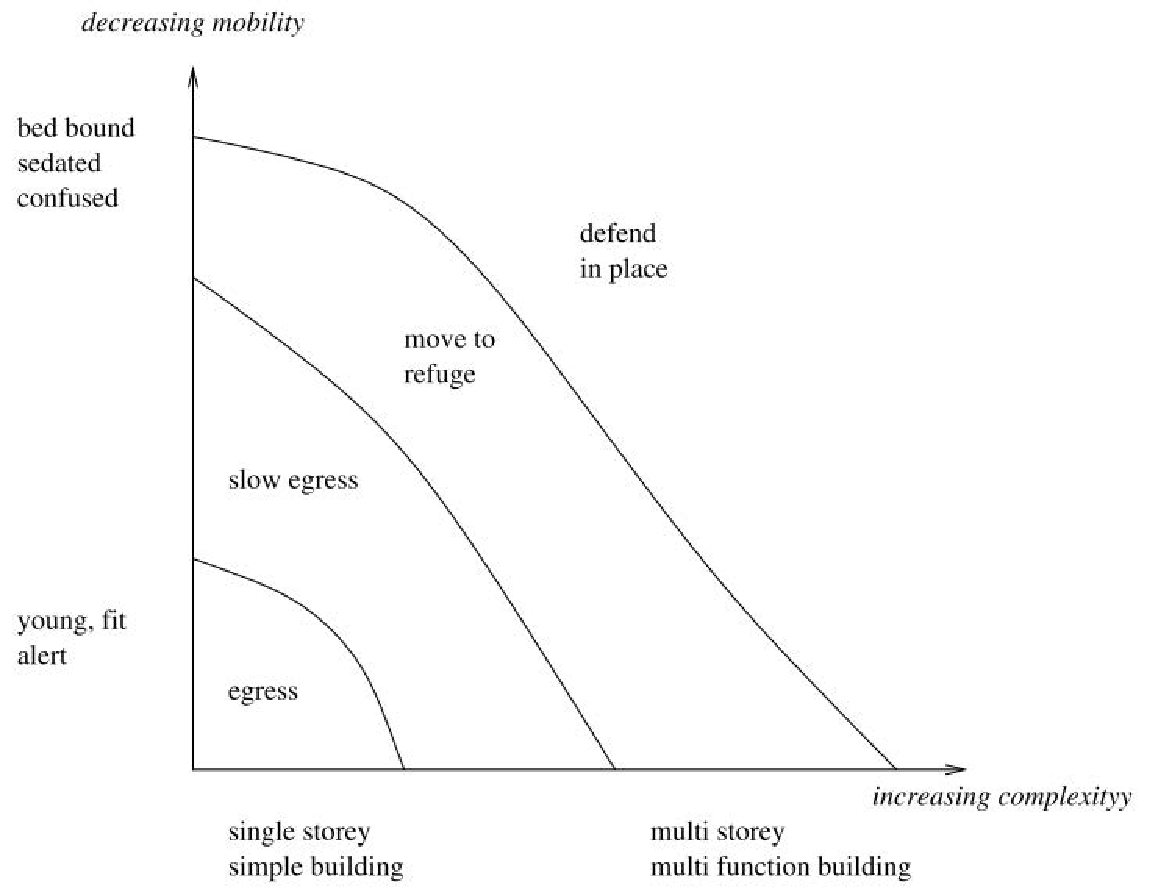
\includegraphics[height=4in,width=\textwidth]{EgressStrategies}
\caption[Strategies for Egress]{According to this chart from~\cite{Klupfel:2005to} there are four strategies that humans resort to in egress. Studies have shown though that more often than not, egress or slow egress are the only strategies taken.}
\label{fig:EgressAge}
\end{figure}

However, it is important to note that flight behavior is not equivalent to competitive behavior characterized by pushing and shoving. The competitive behavior, which is central to the first two models listed above, has been established to be non-existent during egress, at least not in the sense of it spreading through the crowd. Cocking and Drury~\cite{Cocking:2005uc}, who are the main proponents of the self categorization theory, do admit that individual panic does occur; but rather than the panic spreading through the crowd it is the calm people who manage to impose their will on other people and calm the people who panic. The same thoughts were echoed in other studies~\cite{Paulsen:1984ti,Sime:1983uy,Schadschneider:2008cz}. Several studies~\cite{Sime:1983uy,Paulsen:1984ti,Drury:2009ga} actually take a much stronger stand that competitive behavior almost never happens and rather people almost always behave altruistically. This was further confirmed by Torres~\cite{Torres:2010tj} who found that individual competitive behavior never occurred. Nevertheless, people did do whatever they could to enhance their and their groups survival but without knowingly causing harm to others~(which is what competitive behavior/ panic entails).

A further point in favor of the latter four models is the importance that they give to social bonds. For example~\cite{Cornwell:2003uo,Chertkoff:1996vw,Andree:2008td}, among others, have already demonstrated the important role that familiarity plays in behavior during egress. This was reaffirmed by Torres~\cite{Torres:2010tj}, who found that even in cases of extreme danger, people still maintained their social bonds. In fact, as opposed to the non-social model, in the real life evacuation, social bonds never broke down. If people did manage to get out of the fire, they would try to come back or help their trapped group members in some way~\cite{Torres:2010tj,Kobes:2009jx}.

The normative model, affiliative model and the SCT models also recognize the importance of social roles in determining the reactions of people to fire. Many studies~\cite{Proulx:2003tc,Proulx:2001we,Paulsen:1984ti,Sandberg:1997tw,Cocking:2008vv,Tong:1985wn} recognize this. They explain how the employees of a workplace who are trained or prepared, generally try to guide customers to the closest exits. They also indicate that within groups, the leader or caregiver~(e.g.\ teachers or parents leading children) continue to take role of leaders during egress and try to find a safe evacuation path and try to protect their group.

% Another important point to be noted is the importance of inter group and intra group interactions and how these interactions affect the decisions and behaviors of the individuals in them. The emergent norm theory explains these through a process of milling and keynoting. While this theory can explain many situations, there are certain problems with this approach which are explained quite well in~\cite{Reicher:2008ep}. The most notable of this is regarding the extended period of milling that is proposed to take place regardless of time constraints. The current understanding~\cite{Reicher:2008ep} is that each person has an individual identity and a group identity. The group identity and the individual identity are highly interconnected in the sense that each individual influences the group's behavior and vice versa. Whileleaders in groups are important, it does not support the idea of keynoting where only the leader has full power over the group.

In summary, most experiments and studies have been in favor of an affiliative or SCT based model with certain elements of the normative model included. Thus, the consensus is that people always try to escape while trying not to compete with each other and they look for familiar people or locations in dangerous situations and if possible they even form new bonds with strangers stuck in similar situations. Also, the social role of a person determines his behavior. The staff of a place try to ensure safe egress of customers and social leaders~(parents, teachers, etc.) take more responsibility during these times. One of the salient features of a news report of a fire incident or an evacuation of any sort is the irrational and panicking crowd which is discussed in the next section.

\subsection{On the rationality of crowds}
\label{LiteratureReview:RoleOfStress}

 It has been proved~\cite{Kobes:2009jx,Schadschneider:2008cz,Reicher:2008ep,Torres:2010tj,Paulsen:1984ti,Sime:1983uy} that very rarely do people panic and behave irrationally in spite of time constraints and stress. However, situations have been observed where people do not take the best possible actions and do not act in their best interests~\cite{Sandberg:1997tw}.This is probably because people's rational thinking is bounded by the constraints of their knowledge of the environment i.e.\ they are only bounded rational. Bounded rationality is an idea that is becoming increasingly popular in behavioral economics and it implies three major things~\cite{Jones:1999tn}:

\begin{enumerate}
\item People do not know everything.
\item People cannot think infinitely into the future. They think in the short term and tend to take decisions that benefit them in the short term.
\item People are generally loss averse i.e.\ they do not like to take a risk of loosing more even if the gains are much higher. In a fire evacuation this means that people avoid action for small problems and take drastic actions as things get out of control. This is because early action might result in huge losses~\cite{Graham:2000vl}.
\end{enumerate}

If they are only bounded rational and they tend to make worse decisions as the fire gets worse, then it implies that the time pressure and stress must play some part. Ozel~\cite{Ozel:2001tn} proposed a decision making theory which explains this. The basic premise of his theory is that given the same set of information, people may attend to information differently depending on the stress and amount of time pressure they experience. When people gain information they feel less stressed. This can also explain why people investigate and try to gain more information when they perceive the first few ambiguous cues of fire.

One of the significant ideas suggested by Ozel~\cite{Ozel:2001tn} that could be key to creating an accurate model of egress is the idea of filtration. According to this, to cope with time pressure and unavoidable conditions, people try to filter out all the cues that they deem as unimportant or less important. The rate of this filtration increases as the time pressure increases and as a result cue utilization decreases. This in turn implies that they have lesser information about the environment and tend to behave less rationally. This effect has also been observed by Davis et al.~\cite{Davis01122009} in older people who, due to age, are only able to process less information. The significance of information in egress and more particularly perception will be explained in more detail in Chapter~\ref{chapter:IBP}.

Thus it is understood that humans act rationally within the bounds of their knowledge. However, as the situation worsens, their behavior tends to look more irrational to an observer. This is because the evacuees observe less on being stressed and as a result have lesser knowledge; This in turn results in, what appears to be, irrational actions.

\subsection{Summary}
\label{LiteratureReview:PsychSummary}

To summarize this section, some of the important features that characterize an egress are:
\begin{itemize}
\item Ambiguous Cues: most cues are ambiguous in nature and they need to be present for a certain period of time before catching someone's attention enough for them to even start investigating.
\item Early investigative behavior: Early movement is characterized by investigation rather than egress. The investigators then gain knowledge or information either from what they observe directly or from what they hear from others. So there is a \emph{spread of information} in the environment~\cite{Fahy:2010to,Purser:2001ts}.
\item Flight behavior: Once people interpret the situation as fire, they react to it by trying to get out of the building. They do not try to fight the fire or to seek shelter unless they are forced to by the circumstances.
\item Search for familiarity: People's first action while trying escape is to move around and try to find their primary group members who they are familiar with. They then try to exit through some exit that they are familiar with rather than observing new signs. The search for familiarity, also implies the importance of groups and social bonds, to the extent that even after exiting the building, people might come back to help people from their group.
\item Absence of competitive behavior: People do not engage in competitively pushing or shoving others when engaging in egress. The rare cases when pushing or shoving occurs, it is because the individual involved is forced to do so.
\item Altruistic behavior is common: People tend to help others who need help. They also do not panic or act irrationally. Instead, they follow social norms and try to be as orderly as possible.
\item Decisions and behaviors are dynamic: As people interact with the environment and the other people in the crowd their decisions and behavior might change or be influenced.
\item Bounded Rationality: Stress and time constraints cause a reduction in cue utilization and information availability and thus cause people to make decisions that with complete information will seem irrational.
% \item Groups are important: Groups and social bonds form an important part of determining the person's behavior and decisions. People within a group exchange information and groups also pass on information to other groups. Each group then makes decisions based on the groups intrinsic properties and the information available to them which in turn is determined by the characteristics of the individuals who make up the group. Most groups also have a leader who takes the lead in trying to make decisions.
\end{itemize}

In this section the behavior of humans during fire evacuations has been presented and the factors discussed has been summarized above. In the next section, some of the computation models that have been developed over the years are presented. These models are analyzed against the understanding of human behavior that has been presented in this section.

\section{Computational Models of Egress}
\label{LiteratureReview:EngineeringModels}

Conducting experiments and analysing an environment or an event for it's safeness can be expensive and, more importantly, quite dangerous. Through modeling and simulation,  it might be possible to prevent the unnecessary loss of life. It can help architects design buildings better and the management and fire fighters to handle situations better. To be of most use, these models have to be able to accurately simulate how humans behave. A good predictive model can also help test the existing theories of human behavior through the study of emergent behavior. In the previous section the reader was introduced to psychology and sociology literature on how humans and crowds behave in fire and other evacuation scenarios. In this section, computational models of egress that have been developed over the years will be introduced. Section~\ref{LiteratureReview:ComponentsOfAModel} introduces the different components that generally constitute a computation model of egress. Section~\ref{LiteratureReview:ExistingModelsSummary} presents a broad overview of the different kinds of modelling approaches along with some of their strengths and weaknesses. Finally, Section~\ref{LiteratureReview:DetailedModels} explains in more detail some selected models.

\subsection{Components of a computational model of egress}
\label{LiteratureReview:ComponentsOfAModel}

Depending on the purpose of the model, the approach used and the level of detail, a model can consist of various components and sub-components. At the most basic level each model will have: a model of the environment and a model of individuals involved.

\subsubsection{A model of the environment}

Most models have an environmental model that represents the physical environment of the location where egress is taking place. They may be continuous or discrete and generally consider a single floor with passageways seperated by walls. Doors are almost never modelled. At a lower level, depending on the scale of the simulation, in room obstacles like pillars or furniture are also sometimes simulated. Some models do consider multi storey environments. However, movement along staircases and escalators is more complicated and generally ignored except in rare cases~\cite{Kinsey:2009tg,Klupfel:2003wa}.


An important point of difference is generally the resolution of the environment. Coarse network models have entire rooms as their smallest entity and cannot predict within room complexities of movement, while others have fine networks, which can predict within room movements through the division of the rooms themselves into fine grids. Even this minor approximation is avoided in models that use continuous space. These models can thus model the entire complexity of motion and interaction between the evacuees.

It is also useful to have some model of how the fire or smoke will spread within the environment. In some cases, this can be done by creating a separate external model of the fire or smoke and importing it for the simulation or it can be done in the same model and simulated in parallel with the model of egress. Olenick and Carpenter's report~\cite{Olenick:2003daa} gives a compilation of different models that are used for modeling and simulating fires. In general, however, calculating smoke spread in a simulation is computationally expensive and is not often done.



\subsubsection{A model of the individuals engaging in egress}

This is the most important part of the model and there are a wide variety of ways in which this is done. These will be discussed in more detail in Section~\ref{LiteratureReview:ExistingModelsSummary} and Section~\ref{LiteratureReview:DetailedModels}. There are a variety of things to be considered when a human is being modeled. These include:

\begin{itemize}
\item \textbf{Physical Representation}: This refers to the physical characteristics of the humans being like the shape and size of the model used. This is discussed in much detail in~\cite{Langston:2006kw,Still:2000tp}. Some papers suggest that for accurate modeling an elliptical shape is best but to make this computationally efficient a 3 circle model can also be used like in~\cite{Thompson:1995tm,Langston:2006kw}. The speed of movement of the humans and the time taken for pre-evacuation behavior can also be considered to be part of the physical representation. This is also extensively discussed in some surveys~\cite{Fahy:2010to,Proulx:1995wq}.

\item Navigation: Navigation refers to how the agents move within an environment. Depending on the scale of the environment, this generally consists of a higher level path planning which is generally A-Star and a lower level collision avoidance algorithm. The choice of collision avoidance algorithms can have significant effects on the dynamics produced and this is discussed in more detail in Chapter~\ref{chapter:MotionPlannerComparison}. Movement during egress can have complications because of the effects of fire and smoke on visibility and following behavior~\cite{Kobes:2009jx,Isobe:2003ep,Nagai:2004kl}.

\item Knowledge: Knowledge can refer to either knowledge of events or knowledge of the environment/ layout. Most models assume complete knowledge of both. However, there are some that do model individual specific knowledge and exchange of information. These will be discussed in more detail later.

\item Behavior and decision making capacity: This refers to the detail in which some of the behavior mentioned in Sect.~\ref{LiteratureReview:PsychSummary} is modeled. This also refers to the social interactions that takes place between the evacuees. Some models do not consider behavior at all, while others have sophisticated models of decision and behavior. The same behavior can sometimes be produced by using different techniques. Some models use a functional analogy, like social forces, which approximate behavior through mathematical formulas. While others use rule based techniques.

\item A model of trained staff: It is generally recognized that the employees of a place or the people trained in handling a fire evacuation have a key role to play during egress~\cite{Paulsen:1984ti,Aguirre:2004tn,Andree:2008td,Proulx:2001we}. Some models do take this into account. Recently, there have also been computational models studying the effect of signboard on evacuation.

\end{itemize}

In the following sections, some of the different approaches that are used for modeling crowd evacuation is presented. Not all models have all the components mentioned above, but most models have at least a few of them.

\subsection{An overview of existing computational models}
\label{LiteratureReview:ExistingModelsSummary}

There are a lot of reviews of computational models of egress. Some~\cite{WattsJr:1987tx,Gwynne:1999vi,Kuligowski:2005tt,Schadschneider:2008cz,Zheng:2009id} list and attempt to categorize existing models according to their properties. The literature review in Still's thesis~\cite{Still:2000tp} and Santos and Aguirre's article~\cite{Aguirre:2004tn} give comparisons and critical analyses of some of the most popular computation models of crowd egress. The former gives an analysis from a computational perspective while the latter analyses the models from a psychological perspective. Together they form an invaluable source of information on computational models and their strengths and shortcomings.

The different behavioral criteria along which computation models can be differentiated are discussed in some surveys~\cite{Gwynne:1999vi,Kuligowski:2005tt}. Others~\cite{Schadschneider:2008cz,Zheng:2009id} give a comparison of the models based on an engineer's or a modeler's perspective. It gives an idea of the computational complexity of each of these models. Schadschneider et al.~\cite{Schadschneider:2008cz} explained strengths and weaknesses of each approach in more detail, while~\cite{Zheng:2009id} lists the different models of each kind and their features.

As mentioned in Section~\ref{LiteratureReiew:MultidisciplinaryNature}, all these differences can broadly be said to be differences in level of detail. At the most abstract level, we have models that have a coarse network of just rooms connected to other rooms and homogeneous uniform crowd behaving like a fluid. At the most detailed level, we could have an agent based model that considers each individual to be different from every other and with each having its own memory, decision making capacity and behavior, all of which are in turn influenced by their interaction with other people in the group.

In the following pages, some of the typical models of each approach are introduced and analyzed with respect to the discussion in Section~\ref{LiteratureReview:PsychSummary}.


\subsubsection{Network or Queuing Theory based approaches}

These approaches use the coarse network approach mentioned earlier. Nodes are used to represent rooms and passageways and generally any place which can hold people. The arcs in the network represent the gateways or connections through which people move from one node to the other.

One of the earliest models of this kind is Evacnet+~\cite{kisko1985evacnet+}. In this model, the user specifies the capacity and initial content for each node and the traversal time and arc flow capacity of each arc. Queuing theory is then used to calculate the time required to evacuate the building. As in other networks, waiting time, throughput, length and utilization of each arc can also be determined. \cite{Lammel:2009dj} is another example of a similar queuing theory based approach which has a basic ability to show heterogeneity. But this ability is very limited because there is no way that grouping behavior, investigative behavior or effect of time and stress can be modeled. More importantly they do not correspond to a tangible reality~\cite{Bierlaire:2003uj}. \cite{Lino:2009td} is another example of this approach.

\subsubsection{Flow models}

In these models the crowd is assumed to be a fluid and the crowd motion is predicted based on the geographical layout density and velocity of the particles. Schadschneider et al.~\cite{Schadschneider:2008cz} provided an excellent analysis of these kinds of models. The first of these models was Henderson's model~\cite{Henderson:1974ve} according to which the interactions between the pedestrians were calculated using the kinetic theory of gases. One of the theory's main drawbacks was the assumption of energy conservation and Newton's third law being applicable to crowds.

These drawbacks were removed in later models which make use a of a density function. This function was derived from Boltzmann's transport equation that describes the change for a given state as the difference of inflow and outflow due to binary collisions. These later models are also able to distinguish between different groups of particles that had different destinations. These models however fail to work at low densities and cannot model the complex heterogeneity of a crowd~\cite{Bierlaire:2003uj}.


\subsubsection{Environment Control Based Models}
\label{sec:EnvironmentControlBasedModels}

These models are more complex than the above two and generally manage to model some complexity of behavior. The idea behind these models~\cite{Banerjee:2008jh} is that it will be computationally difficult to model a very large environment with a large number of people, each of them instilled with some complex decision making and behavioral ability. So rather than model complex entities, the decision making ability and ``behavior'' of the agents are stored in the environment itself. The location of an agent determines its behavior. Thus, these models can be termed to as being controlled by the environment.

Banerjee et al.~\cite{Banerjee:2008jh,Banerjee:2009jo} propose an environment with various different layers that together store all the information that is needed for the simulation. This reduces the complexity of the agents considerably. The idea of using environments for computation with the agents having limited complexity is one of the oldest and most established in the field of modeling and simulation. Cellular Automation models and lattice gas models have been around for a long time, and a majority of the models of these kinds use what can be termed as \emph{environment control} to implement complex behavior:

\paragraph{Cellular Automata based approaches:}

 A Cellular Automation (CA) model is one in which space and time are discrete. The state space of a CA model is also discrete and finite. In each time step the values of all cells are updated synchronously based on the values of cells in their neighborhoods. Depending on the type of neighborhood (i.e., von Neumann, Moore), and the type of lattice (triangular, square, hexagonal, etc.), the exact number of cells in the neighborhood of a given cell can vary~\cite{Hoekstra:2010}.

 This technique is very popular and has been used in a number of different ways. In~\cite{Gwynne:1999vi,Kuligowski:2005tt} these models are called \emph{fine network models}.
~\cite{Yuan:2007ja} is a typical, simple CA model in which the agent position is updated based on its distance to each possible exit and the density of the crowd at each possible exit. People choosing familiar exits and choosing to stay with their groups is also modeled. However, they use it only for single room evacuation.

One of the drawbacks of a typical CA model like this is that movement is very simple in that they can only move to one of the fixed neighboring cells which are present at fixed angles. This is very limiting when trying to model detailed motion. In~\cite{Yamamoto:2007dc} a real coded cellular automata model is proposed. It is called a real coded cellular automata because of its proposed ability to consider velocities at angles other than multiples of 45 and magnitudes more than a single cell length away~(non discrete velocities). Each time a points location ends up at a point other than one of the grid points, it is assigned one of the 4 neighboring points probabilistically. Some approaches~\cite{Klein:2009} use a hexagonal grid layout instead of square cells. This gives more freedom of motion.

In~\cite{Klupfel:2003wa} slightly more heterogeneity can be modeled since each agent can have a different velocity. Though it is just a movement model, the pre-evacuation time is modeled through the use of a delay parameter specified for each agent. The same thesis suggests that by combining a CA model with a network based model, these models can be used for modeling egress from complicated buildings also.

Most simple CA based models tend to concentrate on movement. As a result most of these models lack any complex behavior simulation.


\paragraph{Lattice gas models:}

Lattice gas models are CA models that make use of a discretized version of the Boltzmann transport equation to model motion~\cite{Marconi:2002ue,Marconi2002,Nagai:2004kl}. They make use of a discretized version of the Boltzmann transport equation for modeling motion. These models do not generally model any complex behavior. In fact they are generally used on a very small scale to study patterns of egress from a single room and to study the effect of different obstacles, number of exits, etc.\ on egress in extremely dense environments. The approach is not appropriate for modeling behavior.

\paragraph{Floor field models:}

Floor field models are more complicated CA models that are more capable because agents can send messages between each other and communicate.

The Extended Floor Field Model~\cite{nishinari2004extended} in which agents interact through virtual traces that act like the pheromones in chemotaxis and the SWARM information model~\cite{Henein:2006jq} which uses multiple floor fields to model transmission of knowledge between agents are typical examples of floor field models. In the SWARM information model, there are multiple static fields on the floor to indicate the different world views. A higher number indicates a more accurate model. At certain points (for example, points where maps are displayed), the agent can upgrade its knowledge to a more accurate model. It also models communication at a basic level. When an agent with a higher index comes in contact with one with lower index, then the lower agent's index is upgraded. Thus it has a basic method of communication and exchange of information. ~\cite{Qi:2011kv} is also a similar model that has a static potential field guiding towards the goal and a dynamically generated interaction field.

The Situated Cellular Automata~(SCA) modeling framework~\cite{Bandini:2007fa} was proposed so that floor field models can be extended to model more complicated behavior by psychologists and sociologists based on their findings. The authors call it a multi-agent systems based approach, but most of the calculation and processing is done by the environment and not the agents, hence we call this also a environment control based model. Each agent in this model has a particular state that he is in, which influences the way he acts. The idea is to allow agents to emit and store messages in specific locations. When agents reach a particular location they react to all the messages present there~(some from other agents, others from the environment). In this way communication and group behavior can be modeled effectively.

While similar models~(especially the SCA model) might, in the future, be extended to model complicated high level behavior of the kind mentioned in Section~\ref{LiteratureReview:PsychSummary} it is not a very intuitive approach. It is more natural for people to think of behavior at an individual level. Programming behavior through an environment requires abstractions that are difficult for all but the most experienced modellers. Due to this limitation it might be difficult for psychologists or sociologists, who are not used to computational models to extend this model effectively.


\subsubsection{Agent based approaches}
% assuming that agents and the MAS approach would have been basically introduced in the chapter on introduction.


 Agent Based Modelling is the preferred approach for modeling complex behavior~\cite{Epstein:1999vn,Bonabeau:2002um,Li:2008wt} because the bottom up approach makes it easier to view and break down problems into more manageable entities. What exactly are agents? Woolridge~\cite{IntelligentAgentsWoolridge} defines agents as a computer system that is situated in some environment, and that is capable of autonomous action in this environment in order to meet its design objectives. He further defines Intelligent agents as those agents that are capable of flexible autonomous action through reactivity, pro-activity and social ability. The agent architecture is the software architecture used for modeling this decision making ability. Specifying an architecture would provide a structure that can be used to break down the complicated process of decision making. There are several frameworks like the Belief-Desire-Intention (BDI) framework~\cite{BDI} and the Recognition Primed Decision (RPD) that provide a structure on which agent based architectures can be developed.

 % Figure~\ref{fig:ExistingAgentArchitectures} shows the architectures of some agent based models of egress that outline the architecture used. Figure~\ref{fig:MASSEgressAgentArchitecture} and Figure~\ref{fig:LinboAgentArchitecture} describe the simulation architecture more than the agent architecture. The behavior model used in MASSEgress is only defined as pseudo-code and the agent architecture itself is not explicitly defined. Luo et al.~\cite{Luo:2008gj} also take a similar approach of describing their model in text with the architecture simply showing the behavior as being a result of the interaction between situational awareness, agent attributes and behavior execution. Shendakar et al.~\cite{BDIModel} do provide the actual BDI based agent architecture that they use for their simulation( Figure~\ref{fig:BDIModelArchitecture}). However, by defining all memory of an agent simply as \emph{beliefs} and actions as \emph{actuators} the architecture oversimplifies complicated problems that need to be analyzed in more detail. This limits the architecture's general usefulness in studying computational modeling of egress beyond the specific way in which it is used.

 For example,~\cite{AugustijnBeckers:2010cr} is a NetLogo based agent based simulation while modeled the effect of \emph{management} and trained staff. This is done by programming officer agents that instruct other agents to leave and give them instructions on how to do the same. This is a relatively simple task in agent based modeling; models that simulate more complicated emotions, behavior, social interaction and decision making are discussed in more detail in Section~\ref{LiteratureReview:DetailedModels}.

\subsubsection{Hybrid approaches}
Most models use one of these different approaches or can be classified into one of these. However, there are certain exceptions that can't easily be classified as any of these. For example, the pedestrian motion model proposed in~\cite{Bierlaire:2003uj} is a multi agent model that uses a cellular automata at the lowest level for collision avoidance. In fact, it is not even a simple CA model, because it uses a network based representation for path finding and a radial individual specific discretization of space to capture decisions about the direction of walking and the aforementioned CA layer at the bottommost layer.

\subsection{Detailed Discussion of Significant Computational Models}
\label{LiteratureReview:DetailedModels}

The previous section introduced some of the popular approaches to crowd simulation. In this section, models that manage to simulate some of the key characteristics explained in Section~\ref{LiteratureReview:PsychSummary} are introduced.

\subsubsection{Pires's model of pre-evacuation behavior}

Unlike the other models that are described in this section, Pires's model~\cite{Pires:2005gs} is not a complete model of egress behavior. Nevertheless, it is important because it proposes a method by which the pre-evacuation decision making of an individual can be simulated using a simple Bayesian Belief Network~(BBN). It also takes into the consideration the effect of time constraints and stress on the BBN.

However, this approach has its limitations. Most of the details of the pre-evacuation behavior are abstracted away as probabilities which are estimated by \emph{experts}. So, besides not being able to simulate the effect of different kinds of cues, this model does not make it easy to analyze and understand the behavior and movement produced.

\subsubsection{Legion}

Still's Legion model~\cite{Still:2000tp} is based on extensive analysis of crowds exiting stadiums in the UK. The Legion model was extended from the Vegas Model, which worked on the basis of an extensive set of rules that governed the behavior of each agent. Such an approach, Still found, had two basic flaws:
\begin{itemize}
\item One cannot determine, a priori, all the possible conditions that can possibly occur. The same person might have different reactions on different days. As a result, a lot of these specific rules and conditions could be replaced by noise.
\item A lot of behavior can actually emerge due to the self organization of the system, without actually specifying these rules.
\end{itemize}
Still realized that it would be impractical to consider a parameter for smoke, another for nature of threat, another for the emergency and so forth. According to him, during an emergency, a human either moves towards the threat~(investigate), stays in place~(ignore) or moves away from the threat~(evacuate). This choice is based on the value of three parameters that interact- Objective~(try to move to desired or intended end point), Motility~(try to maintain optimal velocity) and Constraint~(try to maintain a minimum distance between yourself and the other objects)- and one parameter that represents the reaction time- Assimilation~(delay in reading and reacting to the environment). He has explained how all the key factors in an evacuation, for example, communication, alertness, social role, position, effect of location, population density and so forth, can all be modeled using just these four factors.

The model is notable for presenting various studies to accurately model the size and shape of human beings. But it comes to the conclusion that a square cell will most accurately model a human being considering the possible ways in which he can turn. Others~\cite{Thompson:1995tm,Langston:2006kw}, however, have shown that an elliptic or a tri-circle model of humans would be more accurate.

Still uses environment control, through what he calls iSpace, for modeling communication between agents. As mentioned in Section~\ref{sec:EnvironmentControlBasedModels}, this approach reduces computational complexity, but at the cost of realistically modeling communication between agents. While groups or clusters do emerge in the model, this is solely the emergent behavior from movement and it is not related to primary groups or particular entities. The perception model is also quite simple and the idea of knowledge spread is not modeled. As a result, even though the idea of emergent behavior is captured brilliantly in this model and a lot of emergent natural phenomena are obtained, it fails to consider pre-evacuation behavior, partial knowledge and the search for familiarity.

The greatest strength of this model lies in the importance given to data, both for theorizing and validation. Also, the physical model used, which was based on an extensive study of the existing data, is something to be emulated. Most importantly, the idea of emergent behavior in crowds was emphasized by the model and experiments. His adherence to Occam's razor in keeping the model as simple as possible and letting more complicated behavior emerge from this is a further strength of this model.


\subsubsection{MACES + PMFServ}
\label{MACESPMFServ}

This model~\cite{Pelechano:2005vp} is most notable for the approach taken to modeling complex behavior. In order to obtain believable emergent behavior a popular psychological model of human beings~(PMFServ) was integrated into their existing Crowd Simulation System~(MACES).

The original MACES model was a multi-agent system based model, with each agent having its own representation of the map. Through exploration and communication they create a more detailed view of the world. This, combined with a model of leadership and non leadership behavior, formed the high level decision making which gave a destination to the lower level path planning algorithm. The lower level path planning algorithm used Helbing's social force model~\cite{Helbing:1995ie} for collision avoidance. This is one of the few models which takes into consideration the partial knowledge of occupants. However, it is assumed that once informed about a room, the agent memorizes and never forgets it. Agents explore in a depth first manner if a path is not known.

PMFserv was conceived as a software system that would expose a large library of well-established and data-grounded Performance Moderator Functions~(PMFs) and Human Behavior Representations for use by cognitive architectures deployed in a variety of simulation environments. Its principal feature is a model of decision-making based on emotional subjective utility constrained by stress and physiology. The basis for this decision making model is Maslov's hierarchy of needs~\cite{Maslow:1943vr} and the OCC model~\cite{Orton:1990tx}. Needs reservoirs corresponding to the degree to which the agent has satisfied his needs are set based on any action that might have occurred in between decision cycles. The OCC model describes a hierarchy that classifies 22 emotion types. Using this hierarchy, the mood of a person in a particular situation can be determined. Besides PMFServ, there are other approaches to emotion modeling for agents as well. For example, appraisal theory based approaches are also used in certain Agent Based Models~\cite{Aydt:2011wz}.

In summary, in this architecture, PMFServ provides the emotional and behavioral basis which is utilized by MACES for motion. Though it has a model of behavior, emotions and decision making it does not model pre evacuation behavior or the search for familiarity. However, it is still of interest to us because of the model of partial knowledge and the idea of having a dedicated and extensible module for behavior with an extensive database of emotions and their effects on decision making. This sort of extensibility is very useful for a behavior model of crowds. In fact, a crowd simulation framework should be flexible enough that different theories of behavior can be used without too much effort. However, one drawback of the architecture used here is that emotions and behavior have no effect on the lower level social forces model. This is a natural difficulty of this approach of improving the model by integrating another existing model instead of having a single central model.

\subsubsection{Collective Panic Behavior Model}

Fran{\c c}a et al.~\cite{Franca:2009wq}, created a simulation model of panic behavior which was based on the hysterical belief theory explained in Section~\ref{LiteratureReview:CrowdBehavior}. To recap, this theory believes that people normally follow social norms and behaviors. A fire alarm or smoke causes social unrest. Following this, people start investigating and communicating with each other and start forming a consensus about what this threat represents. This process of interaction is called \emph{milling}. Following this, a stage of collective excitement is reached wherein a \emph{collective belief~(CB)} is formed between the people and the people no longer have an individual thinking capacity. Next, a social contagion stage is reached wherein the CB is highly contagious and spreads to other people who come in contact with this crowd. After a short period of time, this situation escalates into collective panic where none of the actions of the crowd can be accurately predicted because they are believed to behave irrationally.

Most aspects of this theory of panic have been proven to be wrong as explained in Section~\ref{LiteratureReview:CurrentUnderstanding}. Nevertheless, this model is still interesting due to the detailed way in which the behavior model has been converted into a computation model. Also, the agent architecture is notable for the possibilities it holds for extension.

Each agent is made up of four modules: a Belief and Knowledge Management Module~(BKMM), a Perturbation Module~(PM), Dissipation Module~(DM) and Social Cognitive Module~(SCM). The environment itself is divided into three parts: a physical environment, a communication environment and a group mind representation.
\begin{itemize}
\item
The PM is responsible for picking up cues from the communication environment and analyzing these. These cues are first semantically analyzed using rules specified in the BKMM to determine the mood of the message~(loving, aggressive, neutral). Once analyzed, the information is stored in the BKMM as either a belief or as knowledge based on the amount of evidence for this belief.
\item
On obtaining evidence, beliefs may be changed to knowledge. The knowledge base has three parts to it: The first represents the intrinsic features of the agent~(e.g.\ health, speed), the second represents the knowledge that it gains through perception~(e.g.\ Temperature) and the third represents social state variables that are determined by its interaction with other agents~(susceptibility to other agents). The BKMM also has a rule base that stores information on how to behave and act and interpret information. The rule base itself has three parts: a functional part which gives the agent an identity and goals and instructions to pursue them. A Dynamics module which relies on learning and a reactive module related to the agent's survival which is usually time-constrained. There is a micro representation of the CB in each agent. According to the crowd theory used, there is a tendency for this belief to move towards the macro CB.
\item
Social Cognitive Module is like the control unit of each agent. This module again consists of three parts: Firstly, it has a Cognitive Core module~(CogC) that continuously processes and manages information and guides actions so that the agent can pursue and fulfill its goals. An event that poses a threat triggers the Collective behavior core to take over. This makes the agent act in a collective manner. The trigger is done based on experiences stored in the memory of the agent. Uncertainty about information, due to only partial knowledge, triggers social unrest and milling. During this process, the agent builds up its micro CB representation. As the panic rises, the dynamic rules become less important. The knowledge base has a variable for permissiveness, which represents the adequacy of the actions of the group to the situation. When the actions cross a threshold, i.e.\ they are inadequate for the situation, collective excitement results. At this point, even the functional rules start playing and social norms start being broken. After a certain point, this situation escalates into panic and all the agents act according to the macro CB which enforces a competitive behavior among the agents. The third part of the SCM called communication core is responsible for dispatching instructions from the CogC or CBC to the dissipation module through a queue.
\item
The DM is responsible for sending messages into the environment in the correct format according to the Agent Communication Language. It does so on getting instructions from the SCM and adds details to the message like the mood of the message and whether the information is conveyed as a gesture or a speech.
\end{itemize}

Detailed communication between agents is possible through the use of ACL with details of mood and the type of gesture. Agents don't directly exchange information. Instead, the communicating agent dissipates the message into the environment; and autonomous agents check the communication environment in order to check whether the message is relevant for reaching its goal. The BKMM module represents the idea of information processing and uncertainty reduction accurately. However, the theory of panic and collective behavior, on which the model is based, is much debated~\cite{Torres:2010tj, Sime:1995uu}.

Combined with the PM, a model similar to this can in theory be used for modeling all the pre-evacuation behavior that is necessary. While it is possible to make all these extensions, it doesn't seem like the authors have attempted to do this in their model. Also there is no group behavior or search for affiliation. This is expected because the Hysterical Belief approach on which the model is based has no concept of social bonds and their importance). The absence of altruistic behavior and the importance given to competitive behavior are some other drawbacks. The major drawback, however, is the lack of details about the physical model of the agents or the environment or the level of detail used.

\subsubsection{Exodus}

Exodus~\cite{Owen:1996jh} is one of the most detailed and mature evacuation simulation tools available. It has different packages for building, maritime and aircraft environments. The buildingExodus model comprises five core interacting sub-models: these are the occupant, movement, behavior, toxicity and hazard sub models~(see Fig.~\ref{fig:ExodusDiagram}).

\begin{figure}[!htb]
\centering
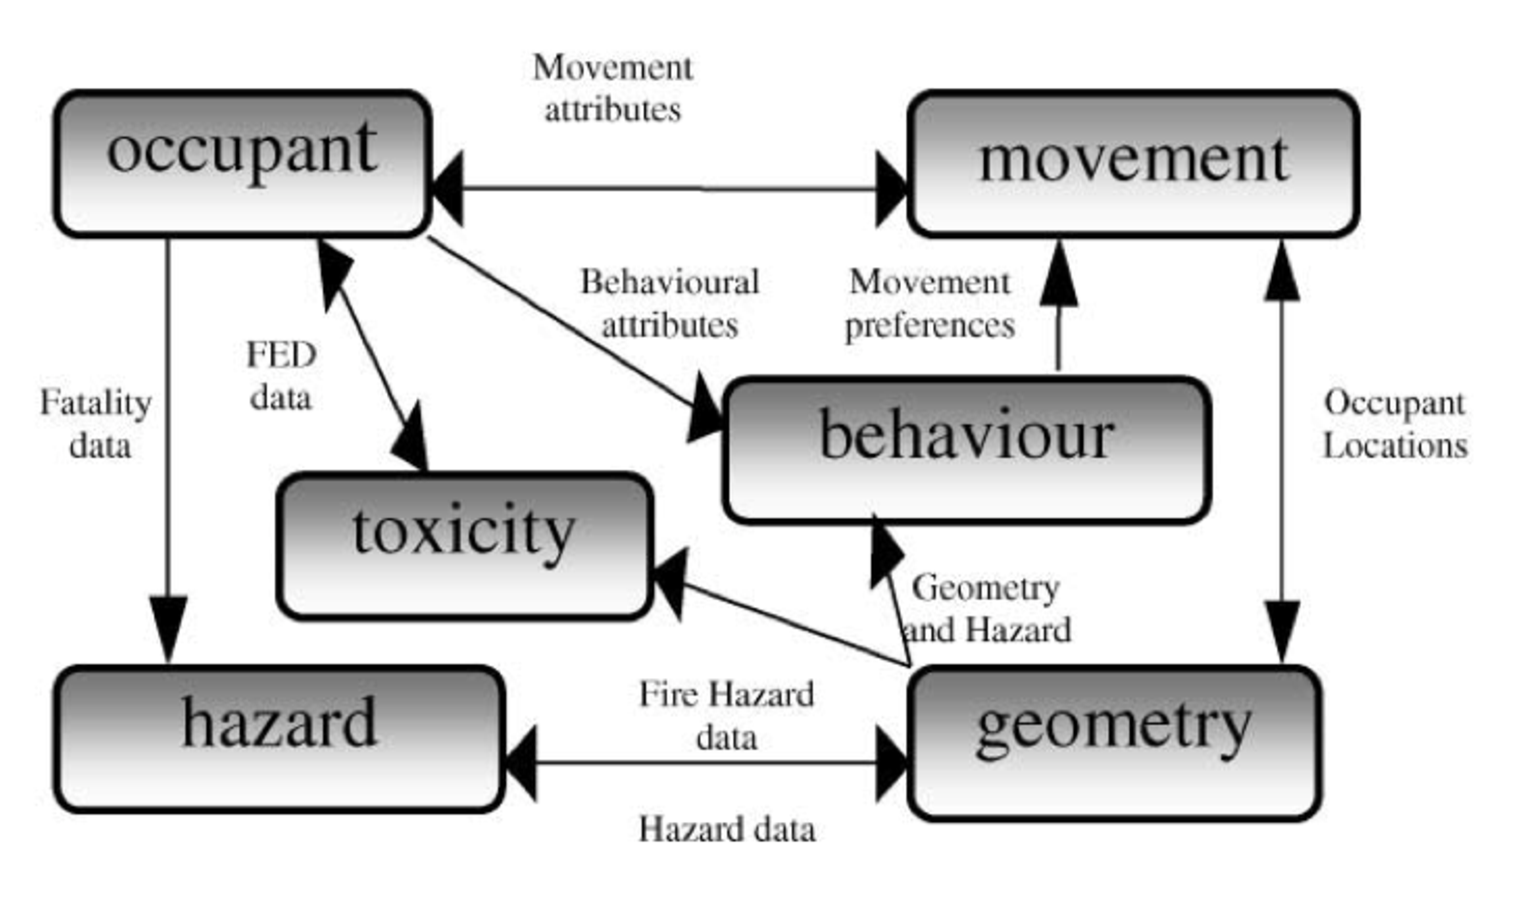
\includegraphics[width=\textwidth]{exodus}
\caption[EXODUS model]{Interaction of EXODUS modules~\cite{Gwynne:2001te}.}
\label{fig:ExodusDiagram}
\end{figure}


Once the building layout is specified as either a DXF file, CAD package, or by using the interactive tools provided in the suite, it is converted into a spatial grid representation which stores all the details of the building including obstacles present inside it. It is also able to store and show movement at staircases and across multiple levels. The grid itself is represented as a graph with the nodes representing a small region of space and each arc representing the distance between each node. Individuals travel from node to node along the arcs.

Each individual has more than 20 behavioral attributes that are specified at the start of the simulation and stored in the occupant submodule. Based on these, the behavioral module determines the behavior of the agents. Two kinds of behavior are modeled: \emph{normal} behavior and \emph{extreme} behavior. The only difference between the two is that in extreme behavior, the agents have a patience threshold beyond which they will stop queuing and resort to some other course of action. The behavior model works on two layers: a global layer and a local layer. The global layer gives a set of waypoints or a single destination~(possibly the exit or a familiar location). The local behavior is determined by the agent's attributes and determines factors like how long he waits before evacuating, conflict resolution and other things. Some of these factors and local behavior are probabilistically determined.

The toxicity submodule determines the physiological impact of the environment on the occupant. This submodule assumes that the effect of smoke or fire is determined by the dose received and not the exposure concentration. The toxicity affects the occupant's mobility agility and travel rates. The hazard module on the other hand is responsible for generating hazards like smoke and fire in the environment as a function of time and location. A dedicated zonal fire simulation model called CFAST is used for this purpose. Several analytics tools have also been developed to analyze the results produced by the simulations.

Gwynne et al.~\cite{Gwynne:2001te} added some new features including the ability to specify occupant specific knowledge of the layout of the building. The behavior module is further modified so that the agent chooses to use emergency exits that he knows of only when he is showing extreme behavior. This representation of a map of the place rather than just a path to exit allows the occupant to dynamically re-plan his route. He is also given the ability to learn from signs and through interactions with other agents.

The effect of smoke is also modeled by reducing the efficiency of the path selected and reducing the speed of movement as per the concentration of the smoke. This reduction in efficiency and speed happens only as long as the exit is not visible to the evacuee. A certain inertia in route replanning is also modeled to indicate the reluctance that people have in changing their pre-decided route.

Hollmann et al.~\cite{Hollmann:2010vy} presented a theoretical prototype of an emotional model that modeled the effect of time pressure and stress on evacuees was introduced into buildingEXODUS. Each agent is specified by giving a list of tasks or waypoints that he has to visit before or during the evacuation. The tasks are categorized as being compulsory time critical and elective and each of them are given an estimated time for completion. An urgency factor indicates how constrained for time the agent perceives itself to be. The speed, drive, patience and the itinerary of each agent is rearranged based on the elapsed time, time left and the feelings of the person. Without an actual implementation of the prototype, it is difficult to analyze the strengths and weaknesses the proposed emotional model.

The strength of the model is the fact that it has a dedicated fire/ smoke simulation engine and a toxicity calculation module. The prototype of the emotion model to be used is also an innovative addition. The ability to specify so many parameters and thus the heterogeneity of agents is also important, as is the ability to model complex building layouts and obstacles in a variety of ways. Nevertheless, the model falls short on a few key factors. It does not try to model crowd behavior or its effects. The idea of cue perception and pre-evacuation behavior is very limited, unless the user specifies a list of tasks that each occupant is to do~\cite{Owen:1996jh}. However, the theoretical prototype fordoing this was never implemented and tested.

The current behavior model is quite limited, with new flowcharts and algorithms and new sets of rules required for each new situation. As discussed earlier, this excessive dependence on specific rules specified is generally considered to be a bad approach~\cite{Still:2000tp}.

\subsubsection{ESCAPES}

ESCAPES~\cite{Tsai:2011tz} is a multi agent based evacuation simulation software tailor-made for airport environments. Unlike most of the other models mentioned earlier, it also has a 3D visualization engine, which makes it more usable for security purposes for non experts. One of the ways in which this model improves on others is that it can model families and social bonds. It models how evacuees search for their family members before attempting to evacuate. Family members also communicate all their knowledge to other family members. It also models a fear factor and emotional contagion.  The knowledge of the fire spreads and the authority figures are able to calm people down. The model also takes into consideration the incomplete knowledge of most people and the spread of knowledge in the environment. However, the models for these are simplistic with only 2-3 states of fear, emotion and knowledge. The reaction time is modeled as a function of the proximity to the event. Agents that are near an event evacuate immediately, whereas others, will behave normally until they get enough information to know that they need to exit.

While the model includes some behavior like affiliation (within families), the prevalence of competitive behavior in the model is unrealistic. The family sizes are fixed~(Parents and two children) and the only social bonds that exist are within this family. The model of partial knowledge is rather simplistic as is the investigative behavior model. Despite these drawbacks, this is one of the few models that consider almost all the factors discussed in Section~\ref{LiteratureReview:PsychSummary}.

\subsubsection{MASSEgress}

Pan's~\cite{Pan:2006vp} multi agent based model of evacuation called MASSEgress is notable for the well structured and detailed architecture of the agents used and the importance that he gives to non-adaptive behavior being synonymous with a high stress evacuation environment.

Mobility, age, gender and body dimension are the only intrinsic characters that are included. A population generator is used to generate the required distribution of people based on these factors. The simulation uses a grid based physical environment which can be loaded as a CAD file. The data from simulation is logged to facilitate easy analysis, and a 2D and 3D visualization engine is also implemented for ease of use and simple analysis. The simulation engine itself simulates the behavior by dividing it into three parts: a perception engine, a behavior engine and a motor engine.

The perception model used is relatively complicated compared to the models discussed above. It consists of a point test method and a ray tracing algorithm implemented along with a visual cone. The visual cone specifies the region in which the agent can perceive and is determined by the eye position, viewing angle and visual range of the agents. The point test algorithm determines whether an exit or waypoint is perceived. The ray tracing algorithm determines which of the obstacles are perceived and ensures that only objects closest to the agent are perceived.

The agent behavior is considered to happen at three levels: an individual level, a group level and a crowd level. At the individual level, an agent generally acts using his experience. If experience can't help then they act rationally within the limits of their knowledge. If they are too stressed, then they start acting on instinct. Instinct refers to competitive behavior where pushing, jumping out of windows and fleeing towards very crowded, blocked exits take place. At the interaction level, a social identity based model is used. Each agent has a social identity and each social identity has a set of actions associated with it. Depending on the situation, the actions taken by an agent are determined by the social identity. Pan assumes that during an extremely stressful situation people forget about their social roles. Personal spaces are defined for each individual which they always try to maintain. If this space is violated, they get agitated and stressed and will eventually lead to \emph{non-adaptive behavior}. The model also assumes a strong herding behavior, where the first reactors influence the reaction of the rest. At the crowd level, the three factors that influence the behavior of an agent are crowd density, environment constraints and perceived emotion and tension. The first two factors are standard in most crowd simulation environments. The third factor is interesting, it states how the individual's perception of a system as stressful determines how stressed he is, not just what happens to him. So even in a non emergency situation, \emph{non-adaptive behavior} might occur if a false alarm or some other stressful situation arises. Queuing, competitive, leader following, altruistic and herding behavior are modeled as resulting from the interaction of these different factors. A decision tree is used to simulate this behavior and to show how each of these behaviors is caused as a result of the aforementioned three levels. The actual implementation of the behavior at an individual level consists of 5 factors: familiarity~(memory), decision making type~(the intrinsic factors determined decision tree), urge to exit, stress threshold type and herding factor.

The movement engine has a simple collision detection algorithm and controls basic movements. Basic movement on stairways are also modeled.

The greatest strength of this model is the way in which the higher level behavior of agents are determined and described using a few fundamental lower level behaviors. It also has a more detailed visual perception system and movement system. However, it does not model pre-evacuation behavior or affiliative behavior of any sort. Like some of the other models, there is an undue prominence of non-adaptive behavior during evacuation.

\subsection{Summary}
\label{LiteratureReview:EngineeringSummary}
In this section, the different types of computational models of fires ranging from network based models to smart environments and agent based models were introduced. Seven existing models that model the key features highlighted in Section~\ref{LiteratureReview:PsychSummary} were also presented and analyzed.
\begin{itemize}
	\item Pires's model~\cite{Pires:2005gs} was one of the earliest to consider pre-evacuation behavior. However, the model abstracted away details of the pre-evacuation behavior as probabilities making it more difficult to study and analyse pre-evacuation behavior.
	\item Still's thesis~\cite{Still:2000tp} highlighted the importance of data. He also, importantly, highlighted the fact it is not necessary to have a complicated model to simulate complex systems. Rather, simple rules may be able to produce the required complex behavior. Models should where possible follow Occam's razor, i.e.\ the simplest rules should be used. This was exemplified by Pan's MASSEgress model~\cite{Pan:2007gb} which produced higher level herding, following and competitive behavior by using simple lower level rules.
	\item Pelechano's work~\cite{Pelechano:2005vp} in combining a dedicated behavior model~(PMFServ) with their existing crowd simulation model~(MACES) demonstrated the importance of inter-disciplinary collaboration. By integrating an existing detailed emotion model to improve an existing computational model, they demonstrated the strengths and limitations of this approach.
	\item The Collective Panic Behavior Model~\cite{Franca:2009wq} demonstrated how a theory of human behavior can be computationally modeled without having to make any abstractions.
	\item The EXODUS model~\cite{Owen:1996jh} is one of the most detailed and mature models today. Hence, it is an excellent source of information on egress modeling and simulation.
	\item ESCAPES model~\cite{Tsai:2011tz} is significant for the importance given to modeling affiliative behavior and the spread of information.
\end{itemize}

\section{Summary of Literature Review}
\label{LiteratureReview:Summary}
This chapter first introduced the complexity of the problem of modeling crowd evacuation and its multidisciplinary nature. In Section~\ref{LiteratureReview:CurrentUnderstanding}, the current theories on crowd behavior during an evacuation were presented with a summary of the salient features required in a comprehensive model of evacuation behavior. Section~\ref{LiteratureReview:PsychSummary} summarized the salient features of human behavior during fire evacuations. In the following section, the different approaches to modeling crowds was introduced and some of the more significant models were presented in detail. Their strengths and shortcoming were summarized in Section~\ref{LiteratureReview:EngineeringSummary}.

 % Despite the variety and number of models available, there is still a lack of a detailed comprehensive model that takes into consideration the latest psychological and sociological theories of crowd behavior. Such a model needs to model the perception of cues and their interpretation; the uncertainty felt by evacuees at the beginning of an evacuation and their search for further information; their preference for familiarity and their search for affiliation and also the effects of stress and time constraints without resorting to the standard assumption of panic/ competitive behavior. In the following chapters, by leveraging on the strengths of existing computational models, a computational model for agents which models these behaviors is introduced.
Despite the number and variety of models available, they all have certain common shortcomings. This chapter has provided a broad look at the computational models of egress and briefly mentioned some of their strenghts and weaknesses. In the following chapter the IBEVAC agent architecture that modularizes the different behavioral components of an agent simulating human behavior. This architecture is used to identify the key problems of existing computational models.

% THe following chapters then take each module at a time.


    %!TEX root = vaisagh_thesis.tex

\chapter{The Building Blocks of a Behavior Model for Egress Simulation}
\label{chapter:IBEVAC}

In the previous chapter, the salient features of the behavior of a crowd engaging in egress were introduced. It is understood that people don't immediately exit a building on hearing a fire alarm or seeing smoke. The occupant gets only an inkling about the danger that is possible. In both these cases there is not enough information for him to get scared and make the decision to egress. If the cues are interesting enough, he then embarks on investigating to gather more information. On realizing that the situation requires some action, he forms a plan to evacuate either alone or, if possible, with his primary group members. In forming this plan of evacuation, unless he is trained for egress or very familiar with the environment, it is unlikely that he will have knowledge of all exits. As a result, he is most likely to just move to the nearest \emph{known} exit. An overview of this process of human evacuation is illustrated in Fig.~\ref{fig:EvacuationProcess}.
% Whatever action they are undertaking, they preserve social norms as far as possible by not shoving or pushing other people~\cite{Cocking:2005uc,Drury:2009ga,Torres:2010tj}.

\begin{figure}[!htb]
\centering
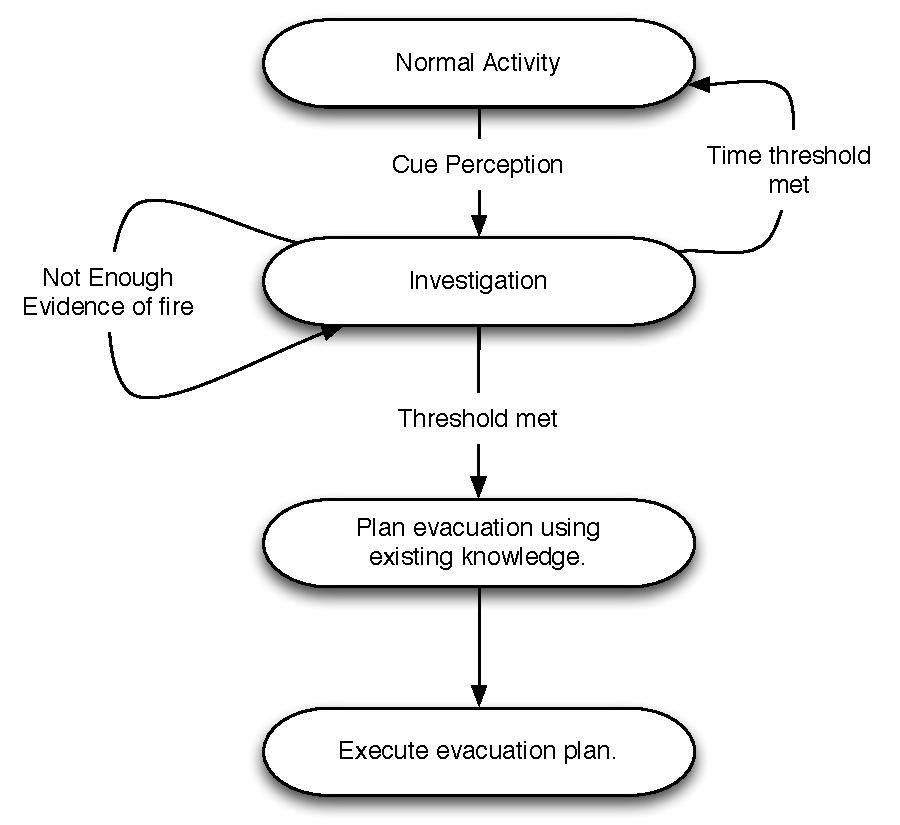
\includegraphics[height=4in]{InfoBasedArchitecture/ProcessOfEvacuation}
\caption[The Process of Evacuation]{The Process of Evacuation: This state diagram shows the different phases of behavior of a person engaging in egress and the triggers that cause phase changes}
\label{fig:EvacuationProcess}
\end{figure}


A small set of core subprocesses and their interaction is necessary and sufficient to produce this evacuation process. These are introduced in Section~\ref{IBEVAC:EgressProgress}. Section~\ref{sec:shortcomings_in_existing_models} introduces some of the shortcomings of existing approaches to modelling each of these sub processes. Section~\ref{IBEVAC:Contributions} explains how these shortcomings are addressed and overviews the key contributions of this thesis.




% section existing_agent_architectures (end)

\section{The Building Blocks of the Egress Process}
\label{IBEVAC:EgressProgress}

The individual behevaior of an evacuee during emergency egress was summarized in Figure~\ref{fig:EvacuationProcess} from the literature discussed in Chapter~\ref{chapter:LiteratureReview}. This section outlines the building blocks of a system that simulates crowd egress during an emergency event. The first step in simulating the behavior of any human being engaging in an activity is modelling his \emph{perception} of the environment. Once perceived, the information gained from perception is used to \emph{identify events} and trigger key actions. In the case of an egress simulation, this would be evacuation (or one of the processes leading up to it). Following this, the person tries to form an evacuation plan using the \emph{knowledge} he has of the layout of the environment and also the information that he is currently perceiving. Once such a plan is formed, a \emph{path is planned} towards this point and he moves along this path towards his goal. Thus the process of egress simulation can be said to consist of four major building blocks: perception, event identification, spatial knowledge utilization and navigation. The following sections defines and explains each of these building blocks and their significance in the evacuation process.

\subsection{Perception}
\label{IBEVAC:IBP}

	Perception refers to the process by which an environment is observed by a person. For an agent, this implies that it should extract features from the environment. These features are called percepts~\cite{Russel:1995vi}. Each percept gives the evacuee certain information about the environment. At the simplest level, percepts provide the agent information about the location and the environment around it and thus allows it move naturally around the environment. In some cases, something out of the ordinary like a ringing fire alarm or smoke or even people running away from a location, might be perceived. Communication between agents can also be considered to be a mode of perception since it is a process by which additional information is gained by the agents. The perception process is the main interface of the agent with the environment through which it gets all the information needed to act. In order to act on information perceived, it is essential for the agent to be able to identify events that require some action.
    % This idea of looking at perception as a process of gathering information is referred to, in this thesis, as \emph{information based perception}.

\subsection{Event identification}
\label{IBEVAC:EventIdentification}

	  In some cases, evacuees might perceive something out of the ordinary like a ringing fire alarm or smoke or even people running away from a location. If these special percepts, known as \emph{cues}, are intriguing enough, then the occupant will set about investigating the environment in search of more cues that would help make a decision on a plan of action. Cues are certain changes in the environment that indicate that something is wrong or different from normal~\cite{Sime:1983uy}. Thus, cues help people identify an event and a need for an action. During emergency egress, on perceiving \emph{sufficient} cues from the environment, an evacuee stops whatever task he's doing and initiates a process of investigation. Once enough evidence is gathered to convince the evacuee of danger, evacuation starts. If enough information is not obtained then the evacuee will likely resume their previous task. Thus identification of events is a key component of the evacuation process that is especially important for modelling pre-evacuation behavior.

    % A person's intrinsic characteristics like age, gender and mental state determine how much information is considered enough i.e.\ the threshold. Each person keeps a track of all the cues that are perceived and when the amount of information crosses the threshold, the evidence is acted upon. In the first phase, this action would be to start investigation and in the second phase it would be the starting of the process of evacuation. In this thesis, this whole process by which the evacuee perceives, analyses and aggregates cues and identifies an event is called \emph{event identification}.

    In summary, event identification is the process by which the evacuee interprets perceived information and decides to proceed to the next phase of evacuation. Executing the action for a particular phase generally requires the evacuee to proceed to a particular location in the environment. This is done using the subjective knowledge that he has of the environment.

\subsection{Spatial knowledge utilization}
\label{IBEVAC:Knowledge}

	On recognizing that there is an event to escape from, the evacuee moves towards the closest known exit. Each evacuee holds his own personal version of the map of the environment which is used for evacuation and movement in general. This personal map is called his cognitive map~\cite{tolman1948}. In most cases, this map is not complete. In a scenario where all known exits are blocked or if the evacuee does not know any exit, he is likely to engage in some sort of exploration behavior which helps increase his knowledge and improve his cognitive map.

    The process of knowledge modelling encompasses the method used for modelling the cognitive map and how it is obtained by the evacuee and his actions when insufficient knowledge is available to act. Modelling evacuee-specific \emph{knowledge} is necessary to model the heterogeneity in behavior found in real life emergency evacuations. The key function of the spatial knowledge model for the agent is to provide it with a target to move to complete the action required based on the event identified. The actual movement towards this point is controlled by the navigation system.


\subsection{Navigation}
\label{IBEVAC:Navigation}

	Navigation is defined as the process or activity of accurately ascertaining one's position and planning and following a route. In the context of egress simulation, we define navigation as the process by which an evacuee first plans his route towards a \emph{goal location} based on his cognitive map and then moves along this route towards the goal. Thus, navigation consists of 2 distinct processes: planning a route and following the route. The former is referred to as path planning and the latter is called motion planning.

    During emergency egress, once evacuation has started, the agent decides that it must proceed to a particular exit, say exit D. Given the current location and this goal, the path planning system recommends a sequence of locations, or waypoints, through which the agent should proceed to get to this goal. Understanding the process of path planning in agent based simulations is easier if it is divided into two parts:  A higher level path finder that finds abstract logical waypoints towards the goal, i.e. go through room A to room B to room C and take Exit D; and a lower level mechanism that translates these logical waypoints to physical locations on the map that the agent can pass through to reach it's goal. Fig.~\ref{fig:detailedNavigationModule}, which gives a mathematical overview of the navigation process, refers to the former as ``Logical Waypoint Determination'' and the latter as ``Current Waypoint Path Determination''. Once these physical waypoints are determined the actual movement towards these locations are determined by the motion planning process.

    Motion planning is a term borrowed from robotics which originally means detailing a task into discrete motions. In the context of crowd simulation, we use the term motion planning to refer to the task of finding a collision free velocity to get from the current point to the next waypoint in the planned path. The motion planning layer ensures that the agent manages to reach its next way point without colliding with other agents.

    Assuming that the cognitive map is modelled as a graph with the edges $E$ representing \emph{areas} or rooms in the environment, Figure~\ref{fig:NavigationArchitecture} gives a mathematical model of how navigation is generally modelled.


    % To explain the working of the navigation module, we make use of the illustration in Fig.~\ref{fig:detailedNavigationModule}.  In this thesis, the cognitive map is implemented as a graph with the edges indicating \emph{areas} or rooms in the environment and $E_i$ refers to an $i^{th}$ edge of the graph in the agent's cognitive map.

    \begin{figure}[!tb]
    \centering
    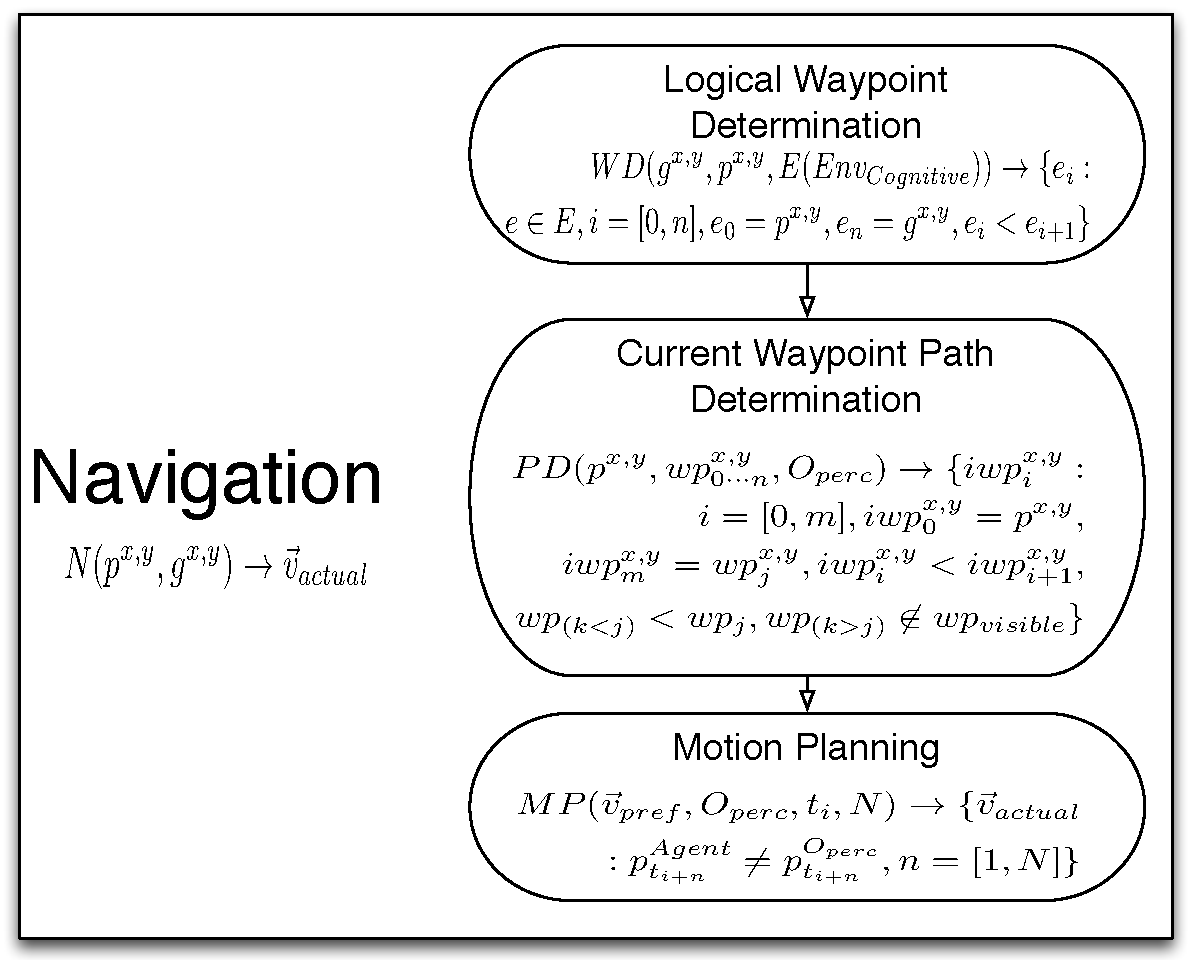
\includegraphics[height=5in]{InfoBasedArchitecture/NavigationWithFormula}
    \caption[Detailed Navigation Model]{Mathematical description of the working of a Navigation System}
    \label{fig:detailedNavigationModule}
    \end{figure}

    The goal position~($g^{x,y}$) is first received by the \emph{Logical Waypoint Determination}~($WD$) system which then uses a route finding algorithm like A-star or Djikstra's to find a set of logical waypoints~($E_i$) that will lead the agent from its current position($p^{x,y}$) to the goal position~($g^{x,y}$). The logical waypoints in the path so planned will be a list of links from the agent's cognitive map~($Env_{cognitive}$). This implies two things: Firstly, it looks at the environment at the room/ area level. Secondly, the agent plans a path according to his personal cognitive map hence there is no garantuee that the path planned by two agents from the same point will be exactly the same. This step is called a waypoint determination step because it returns a set of logical waypoints to be used by the agent to reach its goal. This set of logical waypoints is then passed to the next level of navigation, i.e.\ \emph{the Current Waypoint Path Determination} step.

    The \emph{Current Waypoint Path Determination}~($PD$) differs from the higher layer in that it takes into consideration dynamic obstacles i.e.\ other agents, as well as the static obstacles to determine a collision free path from the current location to the farthest visible waypoint. The logical waypoints are first converted to a set of concrete waypoints~($WP^{x,y}$) which are actual locations on the map. Using the set of perceived obstacles~($O_{perc}$) a set of intermediate waypoints~($IWP^{x,y}$) that would enable a collision free path to the farthest visible concrete waypoint~($wp^{x,y}_j$) is calculated and passed to the next level. This level can also be referred to as the \emph{strategic planning step} since it tries to model how a person strategically moves from one point to another while ensuring that it minimizes collisions with others. Nan's pattern based approach~\cite{Nan:2011vr} and ClearPath by Guy et al.~\cite{Guy:2009gu} are examples of models for this layer.

    The preferred velocity of the agent is then set to the velocity that would lead it to the next intermediate concrete waypoint. Following this, the Motion Planning System like RVO~\cite{Guy:2010ko,Yeh:2008tg} or Social force~\cite{Helbing:1995ie} based methods determine the actual movement of the agent for the next time step of the simulation based on this prefered velocity. At each time step~($t_i$), the motion planning system take a preferred velocity~($\vec{v}_{pref}$) and set of obstacles~($O_{perc}$) (both static and dynamic) as input and outputs a possible velocity~($\vec{v}_{possible}$) that the agent can use to ensure that collisions do not occur for the next $N$ seconds. The two important points of difference from the previous layer is that it has some noticeable effect only when a collision is imminent and that it is very short term (limited to a few time steps) as compared to PD.

    % Since the Motion Planning system works on the basis of perceived obstacles and not actual obstacles, there is a chance, especially in dense environments, that the predicted velocity might cause a collision. In such cases, the lowest level \emph{Physical Consistency Check}~($PCC$) layer ensures that unnatural behavior is not produced. As the name suggests, this layer ensures that physical consistency is maintained and people don't walk through other people and static obstacles in the environment during the next time step~($t_{i+1}$). This is the only layer in the agent that uses the actual map($Env_{actual}$) and actual obstacles($O_{actual}$) instead of the personal cognitive map and perceived obstacles.

    To summarize, the navigation system receives a goal that is passed to the highest level which determines a high level route through the different areas in the environment to the goal; this waypoint is passed to the next level which determines a path towards the current waypoint that avoids dynamic obstacles and calculates the velocity of the agent in order to get to the waypoint while avoiding collisions for the next time step of the simulation.




In summary, a perception system along with event identification, a knowledge model and a navigation system can together be used to produce the entire process of a person evacuating from a building. The function of each of these building blocks is summarized in Table~\ref{tab:BuildingBlocks}. In the following sections, we first identify shortcomings in existing models of these processes and then explain the contributions of this thesis to those areas.

% Requires the booktabs if the memoir class is not being used
\begin{table}[tbp]
\centering
\topcaption{The Building Blocks of Human Behavior during Egress} % requires the topcapt package
\begin{tabular}{p{1.0in}   p{2.1in}   p{2.4in}} % Column formatting, @{} suppresses leading/trailing space
\hline\hline %inserts double horizontal lines
Building Block & Definition & Purpose \\
\hline
Perception  & The process of gathering information about the environment. & Learn about the environment and observe events.\\[3pt]
Event Identification & The process by which the evacuee analyses and aggregates cues and identifies an event.  & Change from one phase to another based on perception and internal state.\\[3pt]
Knowledge Modellings & The process of using stored knowledge to formulate a plan for evacuation. & Determining a goal based on the current spatial cognitive map. \\[3pt]
% Communication & The process of knowledge transfer between evacuees. & Exchange of information between evacuees and management by trained staff. \\[3pt]
Navigation & The routing and movement process. & Handles movement towards the evacuee's current goal. \\[3pt]
% Task Management & Higher level management of strategies and tasks for each phase. & Simplifies the handling of multiple tasks to be completed at each phase of the evacuee's pre-evacuation and evacuation behavior. \\[3pt]
\bottomrule
\end{tabular}
\label{tab:BuildingBlocks}
\end{table}

\section{Shortcomings in Existing Models} % (fold)
\label{sec:shortcomings_in_existing_models}

The previous section identified the core building blocks of an agent based model of emergency egress. In Chapter~\ref{chapter:LiteratureReview}, the salient features of human behavior during egress were identified and summarized in Section~\ref{LiteratureReview:PsychSummary}. In this section, we use this to identify key research questions in each of the core building blocks, where either new modelling approaches or new understanding is necessary.


\subsection{Perception : the lack of a realistic approach}
\label{IBEVAC:PerceptionShortcomings}


    Perception is the process by which agents perceive and gather information about the world around them. It is thus a crucial part of an agent based simulation of crowds. However, in most models, it is standard practice to consider a simple circular or elliptical sensor range. All agents and objects within that sensor range are perceived by the agent. One of the rare exceptions to this is the MASSegress model~\cite{Pan:2006vp} that makes use of a ray tracing algorithm to model perception. The assumptions that an agent can perceive as many objects as are there in the sensor range without any internal limit on capacity~\cite{Miller:1956tr} and that perception is simply a visual process are both simplistic. Another related consequence of the limited information processing capacity of humans is that the human brain tries to chunk similar information to improve it's efficiency. modelling this limited information processing capacity and chunking can produce significant improvements in the realism of crowd simulations. This is demonstrated in Chapter~\ref{chapter:IBP} which introduces an Information Processing Based Perception model which takes this into account.


\subsection{Event identification: modelling pre-evacuation behavior}
\label{IBEVAC:EventIdentificationShortcomings}

    % The Event Knowledge Module stores the agent's beliefs about the current state of the environment.

    Several studies~\cite{Kuligowski:2009un} have shown that humans do not evacuate immediately on hearing a fire alarm. This delay between hearing the alarm and actual evacuation has even resulted in deaths~\cite{Berry:2000us}. This can have significant results on the time to evacuation and the general efficiency of evacuation. However, despite several studies highlighting this, pre-evacuation behavior is hardly ever modeled. In the few instances were it is considered~~\cite{Pires:2005gs,Franca:2009el} , the models are rather simplistic.
    % In essence, there is a need for an agent to keep a track of the phase of evacuatio.
    % Event identification can be considered to be equivalent to the process of associating perceived cues with an experience in a Recognition Primed D.

    Chapter~\ref{chapter:PreEvacuationBehavior} introduces a model for event identification that enables the modelling of pre-evacuation behavior and studying of its effects. Through simulation of certain scenarios, the importance and usefulness of modelling pre-evacuation behavior is demonstrated.


\subsection{Knowledge modelling: the effect of partial knowledge}
\label{IBEVAC:EnvironmentKnowledgeShortcomings}

    On deciding to evacuate an evacuee plans a path towards an exit. Ideally, this plan would be to move towards the closest exit that is known. In most cases, however, say a shopping mall or a hospital, it is highly likely that the majority of the occupants do not know emergency exit locations or the closest exits. How evacuees explore and form their memory in such a situation of partial knowledge is still an open problem.

    Existing simulations either assume complete knowledge or have a simplistic memory model where a single visit is remembered forever. It is unlikely that evacuees have such eidetic memories. Also, it is common to simply take a depth first approach to exploration in case of incomplete knowledge. However, there is no proof whether this is the actual way in which evacuees explore.

    Chapter~\ref{chapter:SpatialKnowledgeChapter} first introduces a game based methodology for studying exploration of indoor environments and how human memory works during exploration. By comparing against a pure random walker, it is shown that humans are in fact more effective explorers than a random walker but not as efficient as is portrayed in existing computational models of egress. The study also revealed some interesting patterns in the strategies used for exploring complex indoor environments.


\subsection{Navigation: analyzing motion planning systems}
\label{IBEVAC:NavigationShortcomings}

    The motion planning system used in an agent based simulation of egress is a key determinant of the kind of behavior produced by the model. The motion planning system used can have a great impact on the patterns of motion produced and the dynamics of the crowd.
    There are several different models of motion planning that have been proposed that sometimes work in very different ways. Each model has its strengths and there are studies that demonstrate their strengths. However, despite the abundance of models, there aren't any standard methods for comparing different models.
    In Chapter~\ref{chapter:MotionPlannerComparison} of this thesis, we quantitatively compare and evaluate existing motion planning systems and determine a metric that can be used for differentiating existing motion planning systems and compare their working against real world data.


% section perception_modelling (end)



% section shortcomings_in_existing_models (end)

\section{Contributions of the Remaining Chapters}
\label{IBEVAC:Contributions}

Following is a summary of the contributions of the remaining chapters:

\begin{itemize}
    \item \textbf{Chapter~\ref{chapter:IBP}:} This chapter presents an Information Processing Based model of perception which was presented at the Cyberworlds 2011 Conference~\cite{Viswanathan:2011uy} and further explored in the extended version published in the Transactions on Computational Science~\cite{Viswanathan:ut}. This chapter additionally contains some validation of the model against real world experimental data.
    \item \textbf{Chapter~\ref{chapter:PreEvacuationBehavior}:} This chapter presents a method for modelling pre-evacuation behavior in emergency egress simulation. The model was presented at the Pedestrian and Evacuation Dynamics Conference in 2012 and published in 2014~\cite{Viswanathan:2012vt}.
    \item \textbf{Chapter~\ref{chapter:SpatialKnowledgeChapter}:} A game based methodology for studying the effect of memory on exploration of complex indoor environments and different exploration strategies used is presented in this chapter. The work done in this chapter has been submitted for review to Nature Scientific Reports.
    \item \textbf{Chapter~\ref{chapter:MotionPlannerComparison}:} The final contribution of this thesis is a methodology for quantitatively comparing different motion planning systems which was also used to compare some popular models against real world data. These findings were published in European Physical Journal B~\cite{Viswanathan2014}.
\end{itemize}


\section{Summary}
\label{IBEVAC:Summary}

% This chapter introduced the IBEVAC Agent Architecture for modelling complex behavior in agent based simulations of crowds. This architecture consists of and \emph{Information Based Perception Module} as a sensor, a \emph{Knowledge Base} consisting of both events and the environment, an \emph{Agent Descriptor Module} which could be used to specify the properties of the agents, a \emph{Planning Module} for planning and a \emph{Navigation Module} and \emph{Communication Module} as actuators. The rest of the thesis develops each of these components to form.

This chapter first summarized the behavior of an evacuee during evacuation from the literature in the previous Chapter. Following this, the four essential building blocks for an agent based simulation of emergency egress was presented. Following this, shortcomings of existing approaches to modelling these parts were identified and the contributions of the remaining chapters was introduced.
	%!TEX root = thesis.tex

\chapter{Information Based Perception}
\label{chapter:IBP}
The aim of this thesis is to create an agent based fire egress simulation that models human behavior as accurately as possible. Agent-Based Models (ABMs) consist of large-numbers of heterogeneous, autonomous entities inhabiting a spatially explicit, partially observable environment; macro level dynamics are said to emerge through the asynchronous interactions among these entities~\cite{Bonabeau:2002um,Epstein:1999vn}. Each of these individual entities will iterate through a sense-think-act cycle, where agents obtain information from their environment through {\em sensing}, make a decision through {\em thinking} and finally carry out their decision by {\em acting}. In many application areas in which ABMs have been applied, including crowd simulation, the emphasis is generally on describing thought processes accurately via rules. However, sensing is a critical aspect in the modeling process and can greatly impact both the individual and emergent properties of the system.

The terms perception and sensing are often used interchangeably in simulation literature. For clarity in explanation, the term {\em perception} is used to define the complete process of obtaining a set of (possibly filtered) \emph{percepts}~\cite{Russel:1995vi} from the environment. {\em Sensing}, on the other hand, is defined as the process of obtaining raw information from the environment; in this definition, and in this model, sensing is a part of perception.

As explained in the previous chapter, the proposed IBEVAC agent architecture is based on the central theme that humans are constantly processing information from the environment. The sense-think-act cycle used in agent based modeling is an excellent representation of the process by which humans get information from the environment, process this information and finally, act based on the decision made. Rather than what a human sees, hears or smells, what is more important is what he can mentally process. In fact, the entire human perception system can simply be considered to be an information processing entity. In this chapter the perception system of the IBEVAC agent based on this idea that perception is the process of gathering information from the environment is presented. This is called an \emph{Information Based Perception}(IBP) system.

Miller's seminal work~\cite{Miller:1956tr} on human cognition revealed two important characteristics of human cognition:
\begin{inparaenum}
\item Humans constantly group together similar data into \emph{chunks} of information.
\item At any given time, a human can only process a limited amount of information.
\end{inparaenum}
For IBP, the assumption is made that this limited capacity results in humans being attracted towards certain kinds of information, e.g.\ a bright light or a celebrity; this, in turn, results in other information in the environment being unnoticed. By organizing information into chunks, humans are able to use their limited information processing capability more efficiently. This ability can manifest itself in different ways. It can be reasonably assumed that during motion planning, humans will process a group of people coming towards them as a single obstacle rather than many individuals. This grouping not only helps the person make use of his limited information processing capacity more efficiently,  it also helps him/~her conform to social norms that instruct him/~her that walking through a group of interacting people would be rude.


This chapter explains and illustrates the working and usefulness of an Information Based Perception system for agents. It's viability is demonstrated through the implementation of a simple moving agent and by incorporating information based processing into the agent's navigation system. Why navigation only? Besides being one of the major components of Agent Based Crowd Simulation, navigation is also a process in which the effects of using a new perception system can be observed easily. The experiments towards the end of this chapter illustrate the significant effects that a modified sensing and perception system can have on an existing \emph{motion planning} algorithm.

The remainder of this chapter is organized as follows: Sect.~\ref{IBP:ReviewPerception} gives some background on how humans perceive the world around them; the IBP model itself is introduced in Sect.~\ref{IBP:Theory}; following this, Sect.~\ref{IBP:MotionPlanning} presents an analyses some of the existing work in motion planning; in Sect.~\ref{IBP:Results} presents the preliminary work done in visual and quantitative validation; finally, Sect.~\ref{IBP:Conclusion} concludes this chapter and gives an overview of the work that needs to be done.

\section{Limits of Human Perception}
\label{IBP:ReviewPerception}
In 1953, Hochberg and McAllister~\cite{Hochberg:1953eh} proposed their theory humans try to group together similar information so that information can be encoded in the simplest possible format. They call this \emph{the simplicity principle}. This idea was further extended by Miller~\cite{Miller:1956tr} originally proposed the idea that, at any given time, humans can only process a limited amount of information. He explained this as the human short term working memory having a limited capacity. Humans are aware of what is in their short term working memory and they arne't aware of what isn't stored in it. To enable humans to store more information in this limited storage space, humans ``chunk'' together similar information. He originally proposed that the short term working memory could hold $7\pm 2$ chunks. Recently, Cowan~\cite{Cowan:2001wi} has argued that this limit is actually $4\pm 1$ for most humans. Thus, even though a person's 5 senses are giving him a constant stream of information about the world, limitations of human short term working memory, force the person to act on the basis of only a fraction of this received information.

But then, which specific fraction of this received information is cognitively processed? Regarding visual perception, some studies~\cite{Itti:2001wa,OReagan:1999wj,Triesch:2003vz} have shown that humans only pay attention to certain salient features in the objects that they see. This results in them not noticing changes in items that are not of interest to them. O'Reagan et al.~\cite{OReagan:1999wj} classified elements as either central interest or marginal interest elements and prove that the internal representation of the visual world is rather sparse and essentially contains only central interest information and not information of objects of marginal interest. The world that we perceive around is a combination of this sparse visual world along with the information in our working short term memory received from our other senses.

Based on these studies, for our model, we make the reasonable assumption that the human brain uses some mechanism to determine the significance of a particular \emph{raw percept}. And the short term working memory stores the most significant information in its limited capacity. It is important to realize that this significance determination is done for \emph{all} information received, regardless of the source. We call this significance, the \emph{amount of information}.

The idea of considering the human perception system as an information processing system is not unprecedented. Broadbent~\cite{Broadbent:1965is} extensively discussed the idea of using information theory for modeling human perception. Various studies were presented that indicate that humans have an upper bound on their capacity for holding information for perception. For a single dimension, this limit is roughly estimated to be about 5-6 percepts. For more than one dimension, the number of discernible alternatives is larger but not as large as would be expected if each dimension was completely independent.

The idea of humans being able to process only a limited amount of information is not new to computer animation either. Hill~\cite{Hill:1999ww} was one of the first to introduce the importance of cognition in sensing. Courty~\cite{Courty:2003hy} used a saliency map based approach and Kim et al.~\cite{Kim:2005ub} used cost-benefit analysis in a decision theory based approach to determining the interest points. Grillon and Thallman~\cite{Grillon:2009hf}, this process of interest point determination was automated. They used criteria like proximity, relative speed, relative orientation and periphery to determine the interestingness of various features.

The majority of existing perception systems, consider perception to be only visual perception. Even in more detailed crowd simulation systems like LEGION~\cite{Still:2000tp} and MASSEgress~\cite{Pan:2006vp} perception is implemented to aid movement by detecting other obstacles and goals to enable planning a path towards the goal and to provide a collision free motion. The simplified IBP System implemented so far and demonstrated in this chapter is similarly limited, i.e.\ the IBP is modeled in the context of collision avoidance. The information which the agents perceive are dynamic obstacles, i.e.\ other agents or groups of agents. However, in the final IBEVAC agent the IBP will also observe events, cues and landmarks from the environment. These will, in turn, be used to learn more about the situation and environment and react appropriately to them.

In the present model, it is not proposed to model all the complexities of human perception and visual cognition, rather an agent based perception model for crowds is presented which can not only show a basic implementation of the idea of information based perception but can be easily extended when required, to model more complicated visual cognition. In order to demonstrate the effect of IBP on an agent's navigation system. It is first necessary to have an idea of existing navigation systems.

\section{Navigation Systems}
\label{IBP:MotionPlanning}

To recap, navigation is defined as the process or activity of accurately ascertaining one's position and planning and following a route. Thus we use the term \emph{navigation} to refer to the complete process of how a person moves from one point to another. Navigation itself can be broadly divided into 3 (or 4 parts) as shown in Fig.~\ref{fig:NavigationArchitecture} extracted from Fig.~\ref{fig:AgentArchitecture}. It was briefly explained in Sect.~\ref{IBEVAC:NavigationModule} and will be discussed in more detail in Sect.~\ref{CFW:NavigationModule}. In this section, \emph{motion planning} is discussed in more detail. It tries to ensure that the human does not go through another human being in the crowd.

\begin{figure}[!tb]
\centering
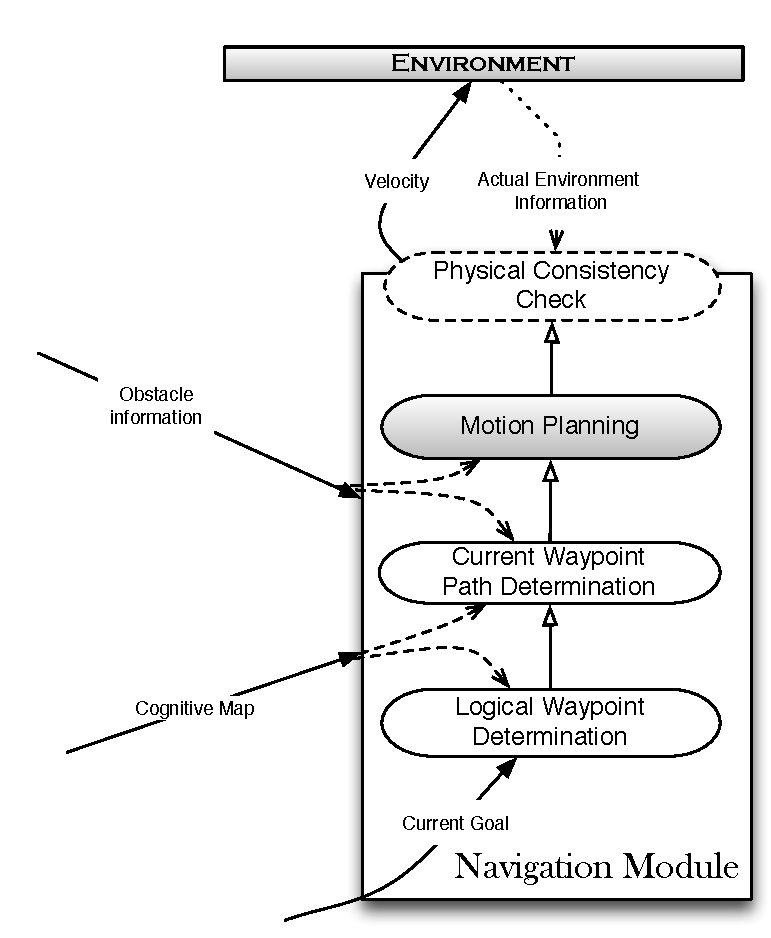
\includegraphics[height=4in]{fig-NavigationArchitecture}
\caption{Navigation Architecture}
\label{fig:NavigationArchitecture}
\end{figure}

There are various different approaches to motion planning. Klein and K\"oster~\cite{Klein:2009} uses an electric potential based model; positive charges are assigned to goals and negative charges to obstacles and agents. Okazaki and Matsushita~\cite{Okazaki:1993wh} use a similar approach of using magnetic poles instead of coulombic charges. In this section, only two of the most popular models for motion planning and collision avoidance used in agent based models, viz. the Social Forces model and the Reciprocal Velocity Obstacle (RVO) model are presented.

The social forces model was first introduced in Helbing's paper~\cite{Helbing:1995ie}. In this model, each agent is modeled as a particle that has multiple forces acting on it. Repulsive forces help in collision avoidance and attractive forces model goal directed and grouping behavior. Over the years, this model has been extended and combined with other higher level behavior models. For example, in~\cite{Kamphuis:2004uu} more complicated group movement was modeled with an underlying social forces model for collision avoidance. In his thesis, Still~\cite{Still:2000tp} criticized the heavily mathematical approach which, according to him, is too complicated to be the natural way in which humans try to avoid crowds.

Another ABM that is increasingly becoming popular for collision avoidance is based on the idea of using the relative motion of objects to determine their time to collision. A velocity is then selected which maximizes this time. This algorithm, based on RVO was first extended for use with multi agent systems in~\cite{vandenBerg:2008cq}. Since then there have been several modifications and improvements to the system but the underlying algorithm still remained the same. CLEARPATH~\cite{Guy:2009gu} which mathematically optimized RVO was the first to introduce a change in the underlying algorithm. Guy et al.~\cite{Guy:2010ko} introduced an entirely new approach to RVO that was based on computational geometry and linear programming. This method further improved the efficiency and smoothness of the system and was called \emph{RVO2}. In another article, Guy et al.~\cite{Guy:2010uv} introduced a personal space factor and an observation delay made the algorithm more appropriate for virtual humans.

Guy et al.~\cite{Guy:2010uv} introduced an extension to RVO in the form of a higher level navigation based on the principle of least effort. While it is obvious that rational humans would prefer taking the path of least effort, as was explained in Sect.~\ref{IBP:ReviewPerception}, humans do not have perfect knowledge or perfect calculation. Also, it is arguable whether humans are always rational enough to choose least effort as their goal.

There are a number of existing motion planning methods that can effectively and efficiently calculate trajectories that avoid all collisions for agents, even in relatively dense environments. For robots and computer games, this might be the ideal goal: perfect, smooth and efficient motion. However, for applications like simulation of emergency evacuation the goal is obtaining realistic motion and not smooth and efficient motion. While humans thrive to be mechanically efficient, this is hardly always the case. There exist, among other things, social norms and limits to mental processing capabilities that prevent individuals from following their ideal preferred path. Also, humans do not necessarily use optimality (in any sense) to determine their preferred path. The approach presented here is a more naturalistic one~\cite{Klein:2009} in that the author feels that motion planning models should explicitly consider and model human inadequacies and limitations.

In this chapter two additions to general motion planning algorithms are proposed:
\begin{inparaenum}
\item Group sensing for motion planning which results in agents avoiding clusters of other agents when choosing their collision free path.
\item Filtering of percepts based on the amount of information provided to model limited information processing capabilities of human beings.
\end{inparaenum}

Another important optimization that was introduced by Guy et al.~\cite{Guy:2010uv} was using the idea of clustering very distant objects into KD-trees to reduce computational cost. While this might sound similar to the idea that is suggested in this chapter, there are two fundamental reasons why this is different from the algorithm presented here: Firstly, the present model uses multiple levels of clustering which will be explained in more detail in Sect.~\ref{IBP:Clustering}. Secondly, the motivation and hence design is significantly different: clustering in IBP is used as a reflection of how agents perceive their environment and not an optimization for collision avoidance.

In the following section a method that will emulate how humans perceive groups whenever possible and a system in which the agents avoid these groups rather than individuals is proposed. This has been done using the Evolving Clustering Method (ECM)~\cite{Song:2001vg} and computational geometry based RVO2~\cite{Wilkie:2009da}. But our approach can, in principle, use almost any clustering and collision avoidance algorithms.


\section{The Information Based Perception Model}
\label{IBP:Theory}

\begin{figure}[!t]
\centering
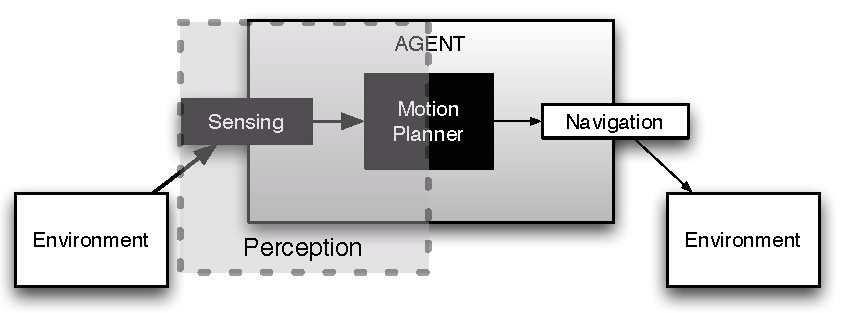
\includegraphics{PerceptionAndActing}
\caption[Perception and Acting]{An agent perceives and then acts}
\label{fig:AgentPerceptionAct}
\end{figure}

This section explains the Information Based Perception System. Figure~\ref{fig:AgentPerceptionAct} illustrates how motion planning works in an agent in terms of a sense-think-act cycle. An agent's perception can be described by a function $ f: Env \rightarrow p*$, where $p*$ is the set of percepts. Each percept $p$ is then processed by the agent in its decision making process, which in turn will determine an appropriate action for collision avoidance. In our case, the motion planning module is passed a set of percepts which consists of neighboring agents and static obstacles which it processes to find the most appropriate velocity for reaching the goal. Typically, this list of neighbors is a set of agents within some cone of vision or some distance away from the agent. In the proposed IBP, a modification to this traditional perception procedure is proposed such that it takes place in three phases: clustering, sensing and filtering. Figure~\ref{fig:AgentClusteredPerception} gives an overview of the process that is detailed in the following sections.


\subsection{Clustering}
\label{IBP:Clustering}
Central to our information based perception system is the definition of \emph{information units}. In traditional crowd simulation each individual agent or obstacle is considered as a percept, i.e. as an entity which should be processed by the motion planning system. The first assumption of our approach is that percepts can be both individuals and groups of other pedestrians. Whether an individual considers a group or individual is related to the {\em coherence} of the group and also the distance of the perceiving agent from the group. In order to achieve this, we perform a global clustering across the entire environment of agents. We create $n_l$ layers within the environment, each layer identifies and stores groups of a particular size, with increasing layer numbers storing groups of increasing size. The criteria which determines what actually constitutes a group is itself unknown and probably highly dependent on the individual. We make the assumption that only the proximity of the individuals to one another determine whether a collection of people is perceived as a {\em group}.

For reasons of efficiency we simplify things by performing a single clustering (for each level) for all agents at every time-step, the consequence is that we are implicitly assuming all agents have the same notion of what constitutes a group. In reality this assumption may be too strong, different people may have different criteria for what they perceive as groups.

While there are various clustering techniques that could be used for grouping agents, we chose to use ECM~\cite{Song:2001vg} because:
\begin{inparaenum}
\item It does not require the number of clusters to be predefined and
\item It can restrict the maximum radius of a cluster.
\end{inparaenum}
It is also important to remember that this clustering is done dynamically at \emph{each step} and not as a one time calculation of groups.


\begin{figure}[!t]
\centering
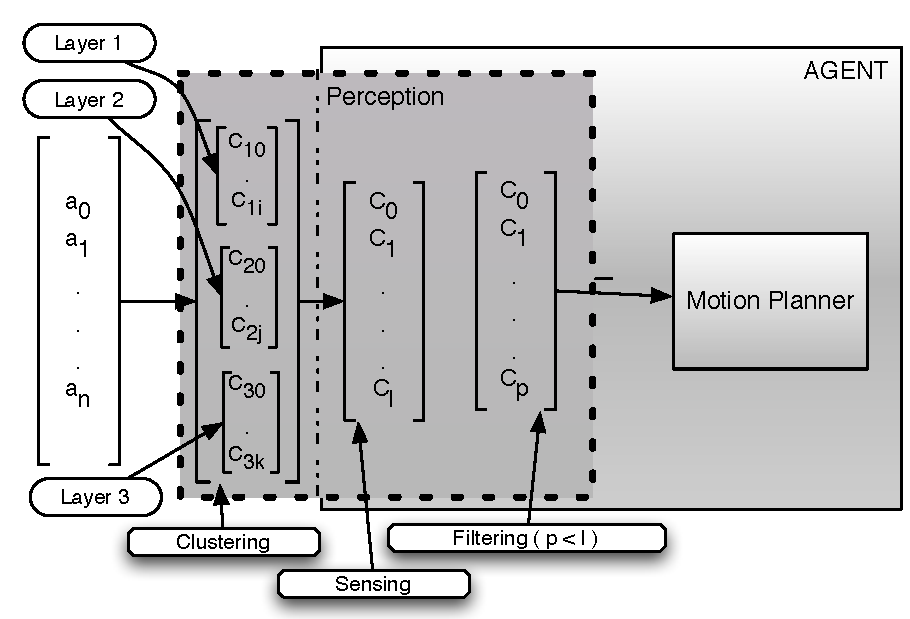
\includegraphics{ClusterProcessing}
\caption[Breakdown of the Perception Process]{Perception in agents takes place through three stages: (1)Clustering is done at a global level. The dotted line indicates this separation. (2) Sensing is the process by which the Agents perceive only a subset of this (3) Filtering further reduces the size of this list and models human visual cognition}
\label{fig:AgentClusteredPerception}
\end{figure}

First the number of clustering layers is decided. In Fig.~\ref{fig:ClusterLayer}, we illustrate information based perception using two layers. The algorithm starts by initializing a single agent as the first cluster, the maximum clustering radius for layer $i$, $r^{i}_{max}$ is fixed (\ref{firstLayerEq} and \ref{secondLayerEq}). Each subsequent agent is then compared with every existing cluster to assess its suitability for addition to that cluster. Suitability is determined by the distance of the agent from the cluster. If the agent lies within an existing cluster, it is simply added to that cluster without updating either the radius or the cluster center. Otherwise, the cluster whose center is closest to the agent is determined. If the agent can be added to this cluster, without exceeding the maximum allowed radius for the cluster, then the agent is added to the cluster and the cluster's radius, center and velocity are updated. On the other hand, if adding the agent violates the maximum radius criteria, then a new cluster is created at the location of the agent.

Once this process is completed for layer $i$, the process is repeated for layer $i+1$ until the clusters for all the layers are determined. This process is illustrated figuratively in Fig.~\ref{fig:AgentClusteredPerception}. The clustering function for layer $i$, $cf_{i}$ allocates one and only one cluster for each agent in each later. This can be represented mathematically as shown below:

\begin{equation}
   \forall a_{k} {\in} A \mbox{ }\exists j \in  [1 , m] \quad cf_{i} : a_{k} {\rightarrow} C_{ij} \mbox{ where } 1 {\leq} m {\leq} n
\end{equation}
\begin{equation}
  \\ \forall a_{j} \in A \quad C_{0j} = a_{j}
\end{equation}
\begin{equation}
 \\r^{1}_{max} = 2 \alpha * r_{a}
  \label{firstLayerEq}
\end{equation}
\begin{equation}
  \\ \forall i \geq 2 \quad   r^{i}_{max} = 2 \alpha * r ^{i-1} _{max}
   \label{secondLayerEq}
\end{equation}

Here $r_{a}$ is the average radius of an agent\footnote{In the experiments at the end of this chapter, it is assumed that all agents have the same radius. Hence, the radius of every agent is the same as the average radius.} in $A$ which is the set of all agents; $C_{ij}$ indicates cluster $j$ in layer $i$; $m$ is the number of clusters and $n$ is the number of agents. $\alpha$ is a parameter that determines the size of clusters and the range of each region (Fig.~\ref{fig:ClusterLayer}). Through experimentation we found the most pleasing results with $\alpha = 2$.

The ECM based clustering for each layer considers each agent exactly once so it the process has an asymptotic complexity of O($n^2$). At the end of each clustering, each agent belongs to a cluster. However, in the absence of nearby agents this might be a singleton cluster.

To correct certain undesirable behavior produced by ECM clustering, a modification was made to the algorithm. With large values of $r_{max}$, there is a chance that distant agents might be grouped into sparse clusters. To counter this problem, we define a \emph{checking circle} as a circle of radius $2 \alpha r_{a}$. If there are no agents within this checking circle, then the cluster is considered sparse and the cluster is removed. The sparseness check is done five times: First with the checking circle centered at the center of the cluster; and subsequently with the checking circles centered at a distance equal to half the distance from the center of the cluster along each of the coordinate axes.

\subsection{Sensing}
\label{IBP:Sensing}

Once the agents have been clustered, the next step is to make use of these clusters for motion planning. As previously explained, existing motion planning algorithms need a list of nearby agents and obstacles to determine the most appropriate velocity. The sensing module of our proposed perception mechanism uses the set of $n_l$ layers created in the clustering module. The list of things to avoid will now consist of agents, obstacles and groups of agents. This list of nearby objects is now calculated from the multiple clustering layers as shown in Fig.~\ref{fig:ClusterLayer}.

\begin{figure*}[!t]
\centering
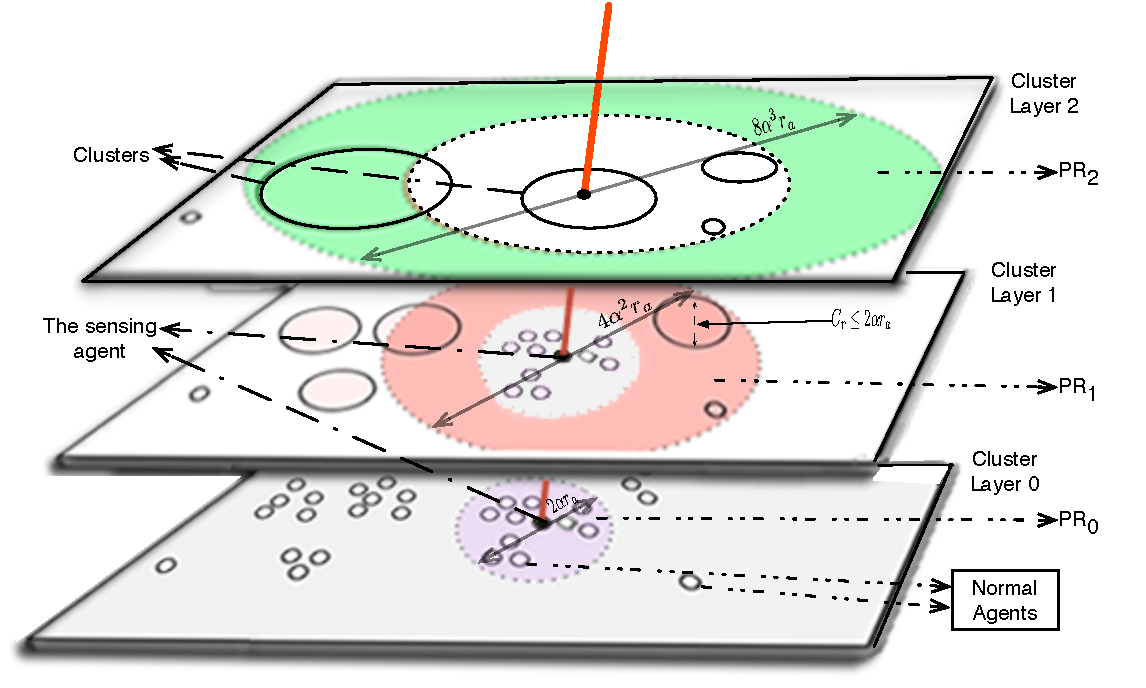
\includegraphics[width=\textwidth,height=3.5in]{AttemptedClusterLayer}
\caption[A Multi-layered Clustering Approach]{The figure illustrates how the opaque agent senses objects using 2 clustering layers. The bottom layer is the original environment and the two planes above show the two clustering layers. Clusters in layer 2 are generally bigger than in layer 1. Solid lined circles indicate the normal agents and the clustered agents. The dotted lines show the regions of perception. }
\label{fig:ClusterLayer}
\end{figure*}


From each cluster layer (explained in Sect.~\ref{IBP:Clustering}) a ring shaped {\em perception region} $pr_i$ is defined for each agent. This region can be considered as a modification of the sensor range which is used in most ABM.  In the first region ($pr_0$), immediately surrounding the agent performing the sensing, the agent perceives other individual agents from the clustering layer 0. This region extends to a distance $r_{pr_0} = 2\alpha *r_{a}$ from the agent's current location. For each subsequent region, the ring shaped region of sensing is from the boundary of the previous layer's region to the boundary of a circle of radius $2\alpha$ times the radius of the preceding region. So for region $pr_1$ the agent perceives groups of maximum size $r^{1}_{max}$, as long as the nearest edge of their minimum enclosing circle is within a distance $d$, such that $ r_{pr_0} < d \leq r_{pr_1}$. The result is a list of obstacles which consists of clusters of various sizes and individual agents.

\subsection{Filtering}
\label{IBP:Filtering}

As explained in Sect.~\ref{IBP:ReviewPerception}, a human being does not cognitively process every single object or obstacle that is within its vision. In other words, an agent can only process a limited amount of information and the information that is processed will be that which is deemed most interesting or important to the agent. So each object in the list obtained from perception is assigned an interestingness score of between 0 and 1 (1.5 for exceptional cases). During the sensing process each agent is given an information limit $a_{IL}$, indicating the total amount of information that can be processed by the agent. This limit is a parameter than can change as the stress level or other characteristics of the agent changes~\cite{Ozel:2001tn}.

For now, it is assumed that interestingness of an object depends on two criteria:
\begin{inparaenum}
\item The distance of the object from the agent.
\item The angle that the object currently forms with the direction of motion of the agent.
\end{inparaenum}
A third factor indicating the innate interestingness of the object being perceived can also be used. This can be used to represent a lot of other properties related to interestingness. For example, an object's speed, color, action or something more subjective, i.e.\ it is of interest only to this agent because of certain properties of the agent. For e.g., for a thirsty agent, a water cooler would be interesting whereas it is unlikely to catch the attention of someone else. A more exact definition of interestingness is not the focus of this report, but the general model here should be able to adapt to more sophisticated definitions. However, a notion of interestingness is required to extend IBP to detect events and cues in the situation and environment and this will be discussed in Sect.~\ref{IBP:Conclusion}.

Based on the two criteria, a score is given to each agent. A distance score of 1.5 is given if the distance between two agents is less than or equal to zero. This is to ensure that in high density scenarios where a collision does occur, a collision recovery mechanism is forced on the objects regardless of what angle or how interesting the object is. For other distances the following equation is used to calculate the score for a distance $d$. $\gamma$ and $k$ are parameters which were fixed at 5.0 and 1.11 respectively to get a curve as in Fig.~\ref{fig:DistanceScore}.
\begin{equation}
  	S_d = max(min(1.0, e^{\gamma / d} - k),0.1)
\end{equation}

\begin{figure}[!t]
\centering
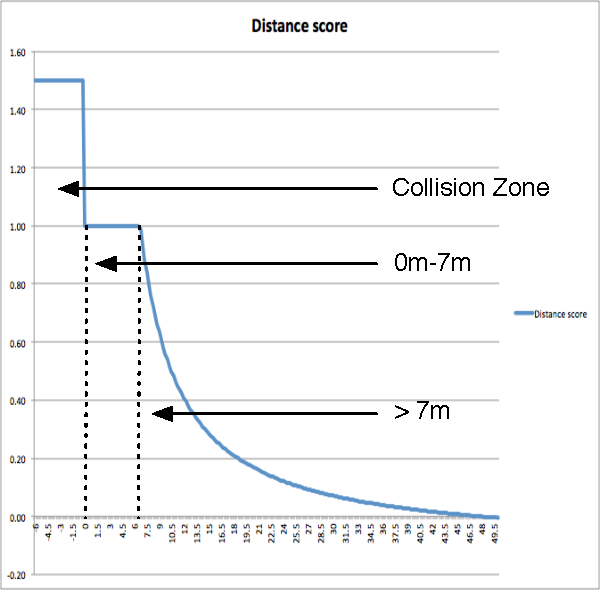
\includegraphics{distanceScore}
\caption[Distance Score]{This graph shows the variation of distance score with distance (in metres) used in experiments. A score of 1.5 if a collision has already occured, a score of 1 if it is within 7m and an exponentially decreasing score beyond that distance}
\label{fig:DistanceScore}
\end{figure}

An angle score of $1.0$ is given to all objects forming an angle of less than $a_{min}$ with the agent's direction. For all agents that form an angle of more than $a_{max} $ with the agent's direction,  a score of $ (1-\beta) $ is given. For our experiments a $\beta$ value of 0.9 was used and this is illustrated in Fig.~\ref{fig:AngleScore}. For all angles in between, the angle score linearly decreases to $ (1-\beta) $ from $1$. This is assigned based on the following equation (Fig.~\ref{fig:AngleScore}). All angles are in radians:
\begin{equation}
	S_{\theta} = 1.0 - (\beta * (a - a_{min} ) / (a_{max}-a_{min}))
\end{equation}

\begin{figure}[!t]
\centering
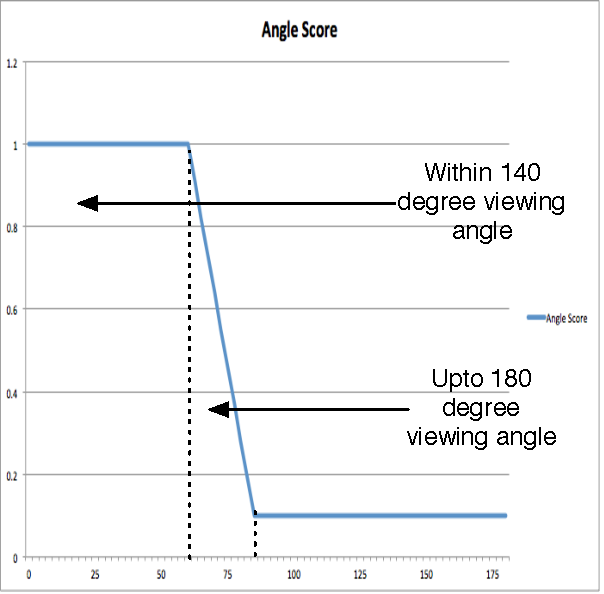
\includegraphics{angleScore}
\caption[Angle Score]{This graph shows the variation of angle score with the angle(in radians) formed by the object with the agent used in experiments. For objects forming an angle of less than $70^{\circ}$ (viewing angle $140^{\circ}$, a score of 1 is given. For objects forming an angle of up to $90^{\circ}$, the score linearly decreases to $0.1$ which is the angle score for all remaining obstacles.}
\label{fig:AngleScore}
\end{figure}

The final score for the object is calculated as the product of the $S_{\theta}$ and $S_d$~(as long as the distance score is not 1.5). This list of objects is then sorted on the basis of the score that is determined. Objects are then removed from the head of this list in turn and added to the final list of perceived objects as long as the cumulative score of all the perceived objects does not exceed the information limit for the agent, $a_{IL}$. All the remaining objects are dropped from the list of objects sensed and the final list of percepts $p*$ is obtained. In case two objects have the same score, the objects that are moving towards the perceiving agent are given precedence, subsequently closer objects are given preference.

This shortened neighbor list is passed to RVO2~\cite{Guy:2010ko} for calculating the velocity at each time step. Our hypothesis is that the 3-step perception process presented in this chapter provides an improvement in two ways: Firstly, there are fewer neighbors and hence, fewer constraints for a given sensor range. Secondly and more importantly, more human like results can be obtained as will be illustrated in Sect.~\ref{IBP:Results}.

\section{Results}
\label{IBP:Results}

Eventually, real world data, which would ideally be used for validation of the IBP model, will be collected. Nevertheless, this section presents a preliminary visual and quantitative validation of the IBP model. The ideas introduced in Sect.~\ref{IBP:Theory} are used as the basis for visually validating different aspects of the proposed model. For quantitative validation of the model, two measures are used: \emph{Effort Expended} and \emph{Inconvenience Cost}. In proposing their least effort based approach to motion planning~\cite{Guy:2010uv}, Guy et al. used a measure of effort expended to demonstrate the usefulness of their model. This effort was calculated as follows:

\begin{equation}
E = m \int \! (e_s + e_w |\vec{v}| ^2) \, \mathrm{d} t \quad \footnote{$e_{s} = 2.23 \frac{J} {Kg s}$ and $e_{w} = 1.26 \frac{Js} {Kg m^{2}}$ for an average human~\cite{Whittle:2006vsa}}
\end{equation}

In this section, the same measure of effort is used to analyze and validate the proposed IBP model. For simplicity, all agents are taken to have the same average mass of 70~kg.  However, this only measures the  mechanical effort involved. To measure the amount of effort spent in decision making, an \emph{inconvenience cost} measurement is introduced. The inconvenience cost is the number of time steps in which the agent chose a velocity other than its preferred velocity i.e., the number of times they had to avoid a collision.

Four different scenarios are considered to evaluate the overall performance. First, the effect that Group Based Perception can have on an agent moving through a crowd is demonstrated and the scenario is visually and quantitatively analyzed. Next, the effect of the multi-layered clustering on an agent moving towards a large group is similarly analyzed. Following this, the necessity of GBP in modeling the information processing limits of human beings is shown. Finally, the importance and relevance of the information threshold is demonstrated by demonstrating the effect that it can have on an agent.

\subsection{Group Based Perception}
\label{GBP}

\begin{figure}[!tb]
  \centering
   \subfloat[Traditional Circular Sensor Range]{\label{Exp1_RVO}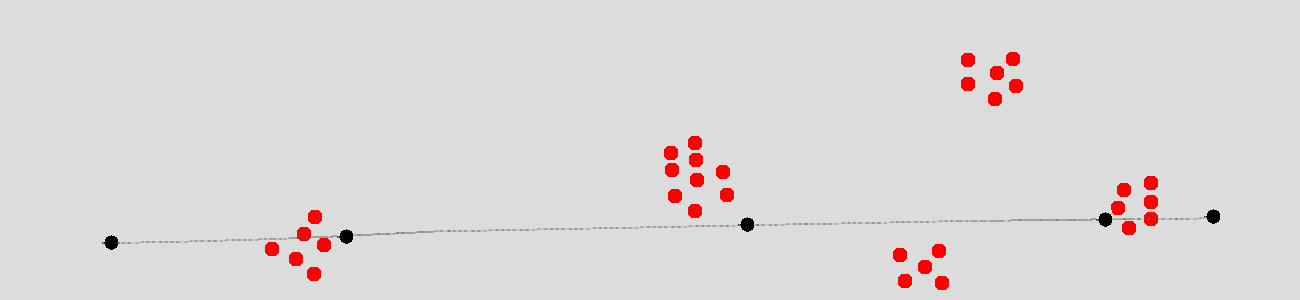
\includegraphics[width=\textwidth]{Exp1_RVO}}
  \\
   \subfloat[Group Based Perception]{\label{Exp1_GBP}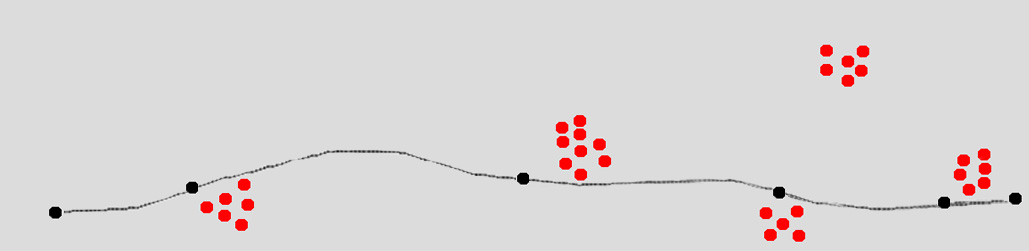
\includegraphics[width=\textwidth]{Exp1_GBP}}
   \caption{Experiment 1: Group Based Perception}
  \label{Exp1}
\end{figure}


In this experiment the results of using RVO2 with a traditional simple circular sensor range against RVO2 with a Group Based Perception system is shown. The intention is to show the effect of perceiving agents as groups. The hypothesis is that by perceiving groups as obstacles the simulation will generate more visually natural motion. In Fig.~\ref{Exp1}, there is a single black agent moving towards the right, and a number of groups of red agents moving towards the left. The black trail shows the path that is taken by the black agent. It can be seen that in Fig.~\ref{Exp1_RVO} where GBP was not used, the agent walked through other groups. Since RVO2 enforces each agent to do half the work to avoid collision, the agents within the group individually give way through its center for the oncoming agent to pass. At present this argument is based on the discussion in Sect.~\ref{IBP:ReviewPerception}, due to social norms and the human tendency to group information together people generally try to move around an entire group rather than walking directly through a group. As shown in Fig~\ref{Exp1_GBP} the GBP algorithm is capable of generating motion which avoids entire groups.

\begin{table}[tbp]
\caption{Quantitative analysis of Group Based Perception}
\begin{tabular}{>{\centering}p{1.2in}>{\centering}p{1in}>{\centering}p{1in}>{\centering}p{1in}>{\centering}p{1in}}
\tabularnewline
\hline\hline %inserts double horizontal lines
\multirow {2}{*}{Agent Considered} & \multicolumn{2}{c}{Effort ($ J{m}^{-1}* 10^5$)} & \multicolumn{2}{c}{Inconvenience Cost}\\
 & Without GBP & With GBP & Without GBP & With GBP
 \tabularnewline
\hline
Black Agent  & 71730 & 71726 & 120 & 148 \tabularnewline
All other agents (average) & 1884 & 1880 & 14.28 & 6.56 \\
\tabularnewline
\hline
\end{tabular}
\label{tab:Exp1_QuantitativeAnalysis}
\end{table}

An analysis of the effort expended and the inconvenience cost gives some interesting results. Since the simulation is executed for a given number of time steps, the effort expended is normalized with the progress towards the agent's goal. This is to avoid slow or stationary agents from being considered to be more efficient despite traveling a lesser distance. On comparing the normalized effort in the two scenarios of the black agent, it is found that despite having a much longer path, the GBP enabled agent expends slightly lesser (practically the same) amount of effort than the other. This is because the non-GBP agent has to slow down to wait for the other agents to give way before it can proceed and thus progresses less towards the goal.

The inconvenience cost comparison gives another interesting, though not surprising, result. The inconvenience cost to the black agent of using Group Based Perception is higher because of the more indirect path that it has to take. However, the average inconvenience caused to all the other agents is significantly lesser. This is consistent with the general human reluctance to inconvenience others. It also gives the interesting idea that even if the same amount of mechanical effort is expended in following two different paths, the amount of decision making required for each path might be significantly different.

\subsection{Effects of multi layered clustering}

\begin{figure}[!t]
  \centering
   \subfloat[Using traditional sensing]{\label{Exp2_RVO}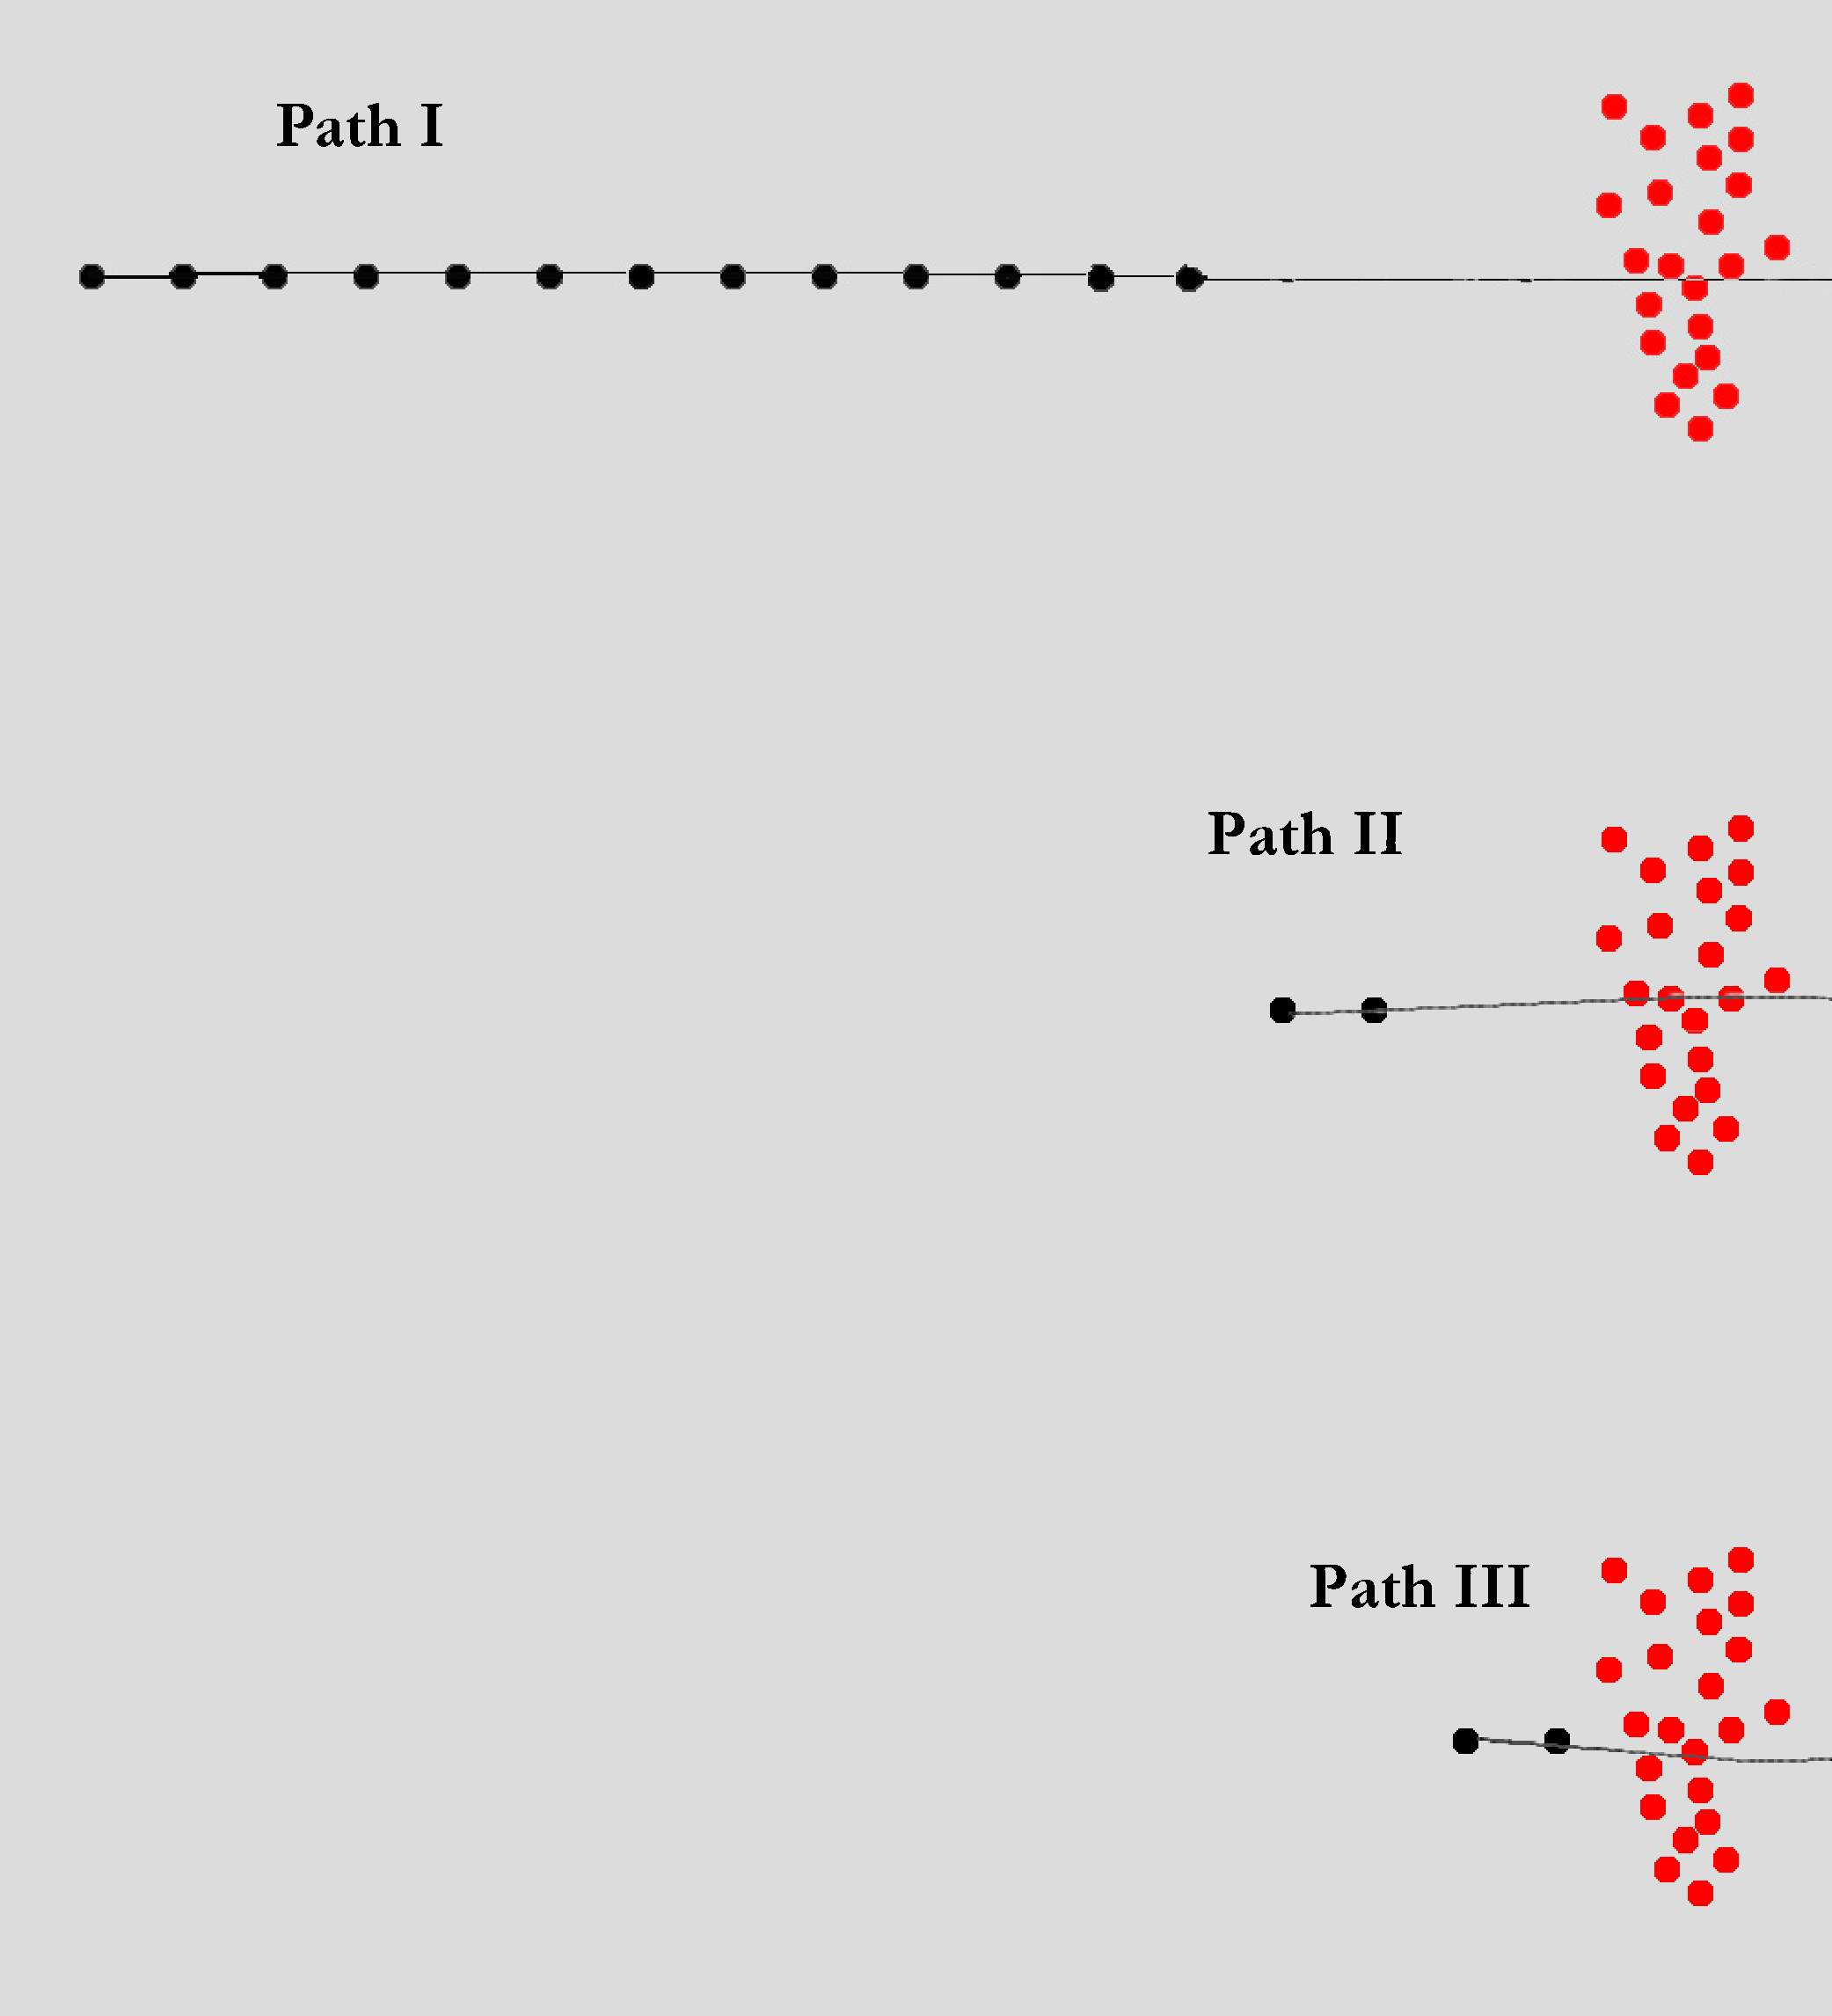
\includegraphics[width=7.5cm,height=12cm]{Exp2_RVO2}}
   \hspace{1pt}
  \subfloat[Using Group Based Perception]{\label{Exp2_GBP}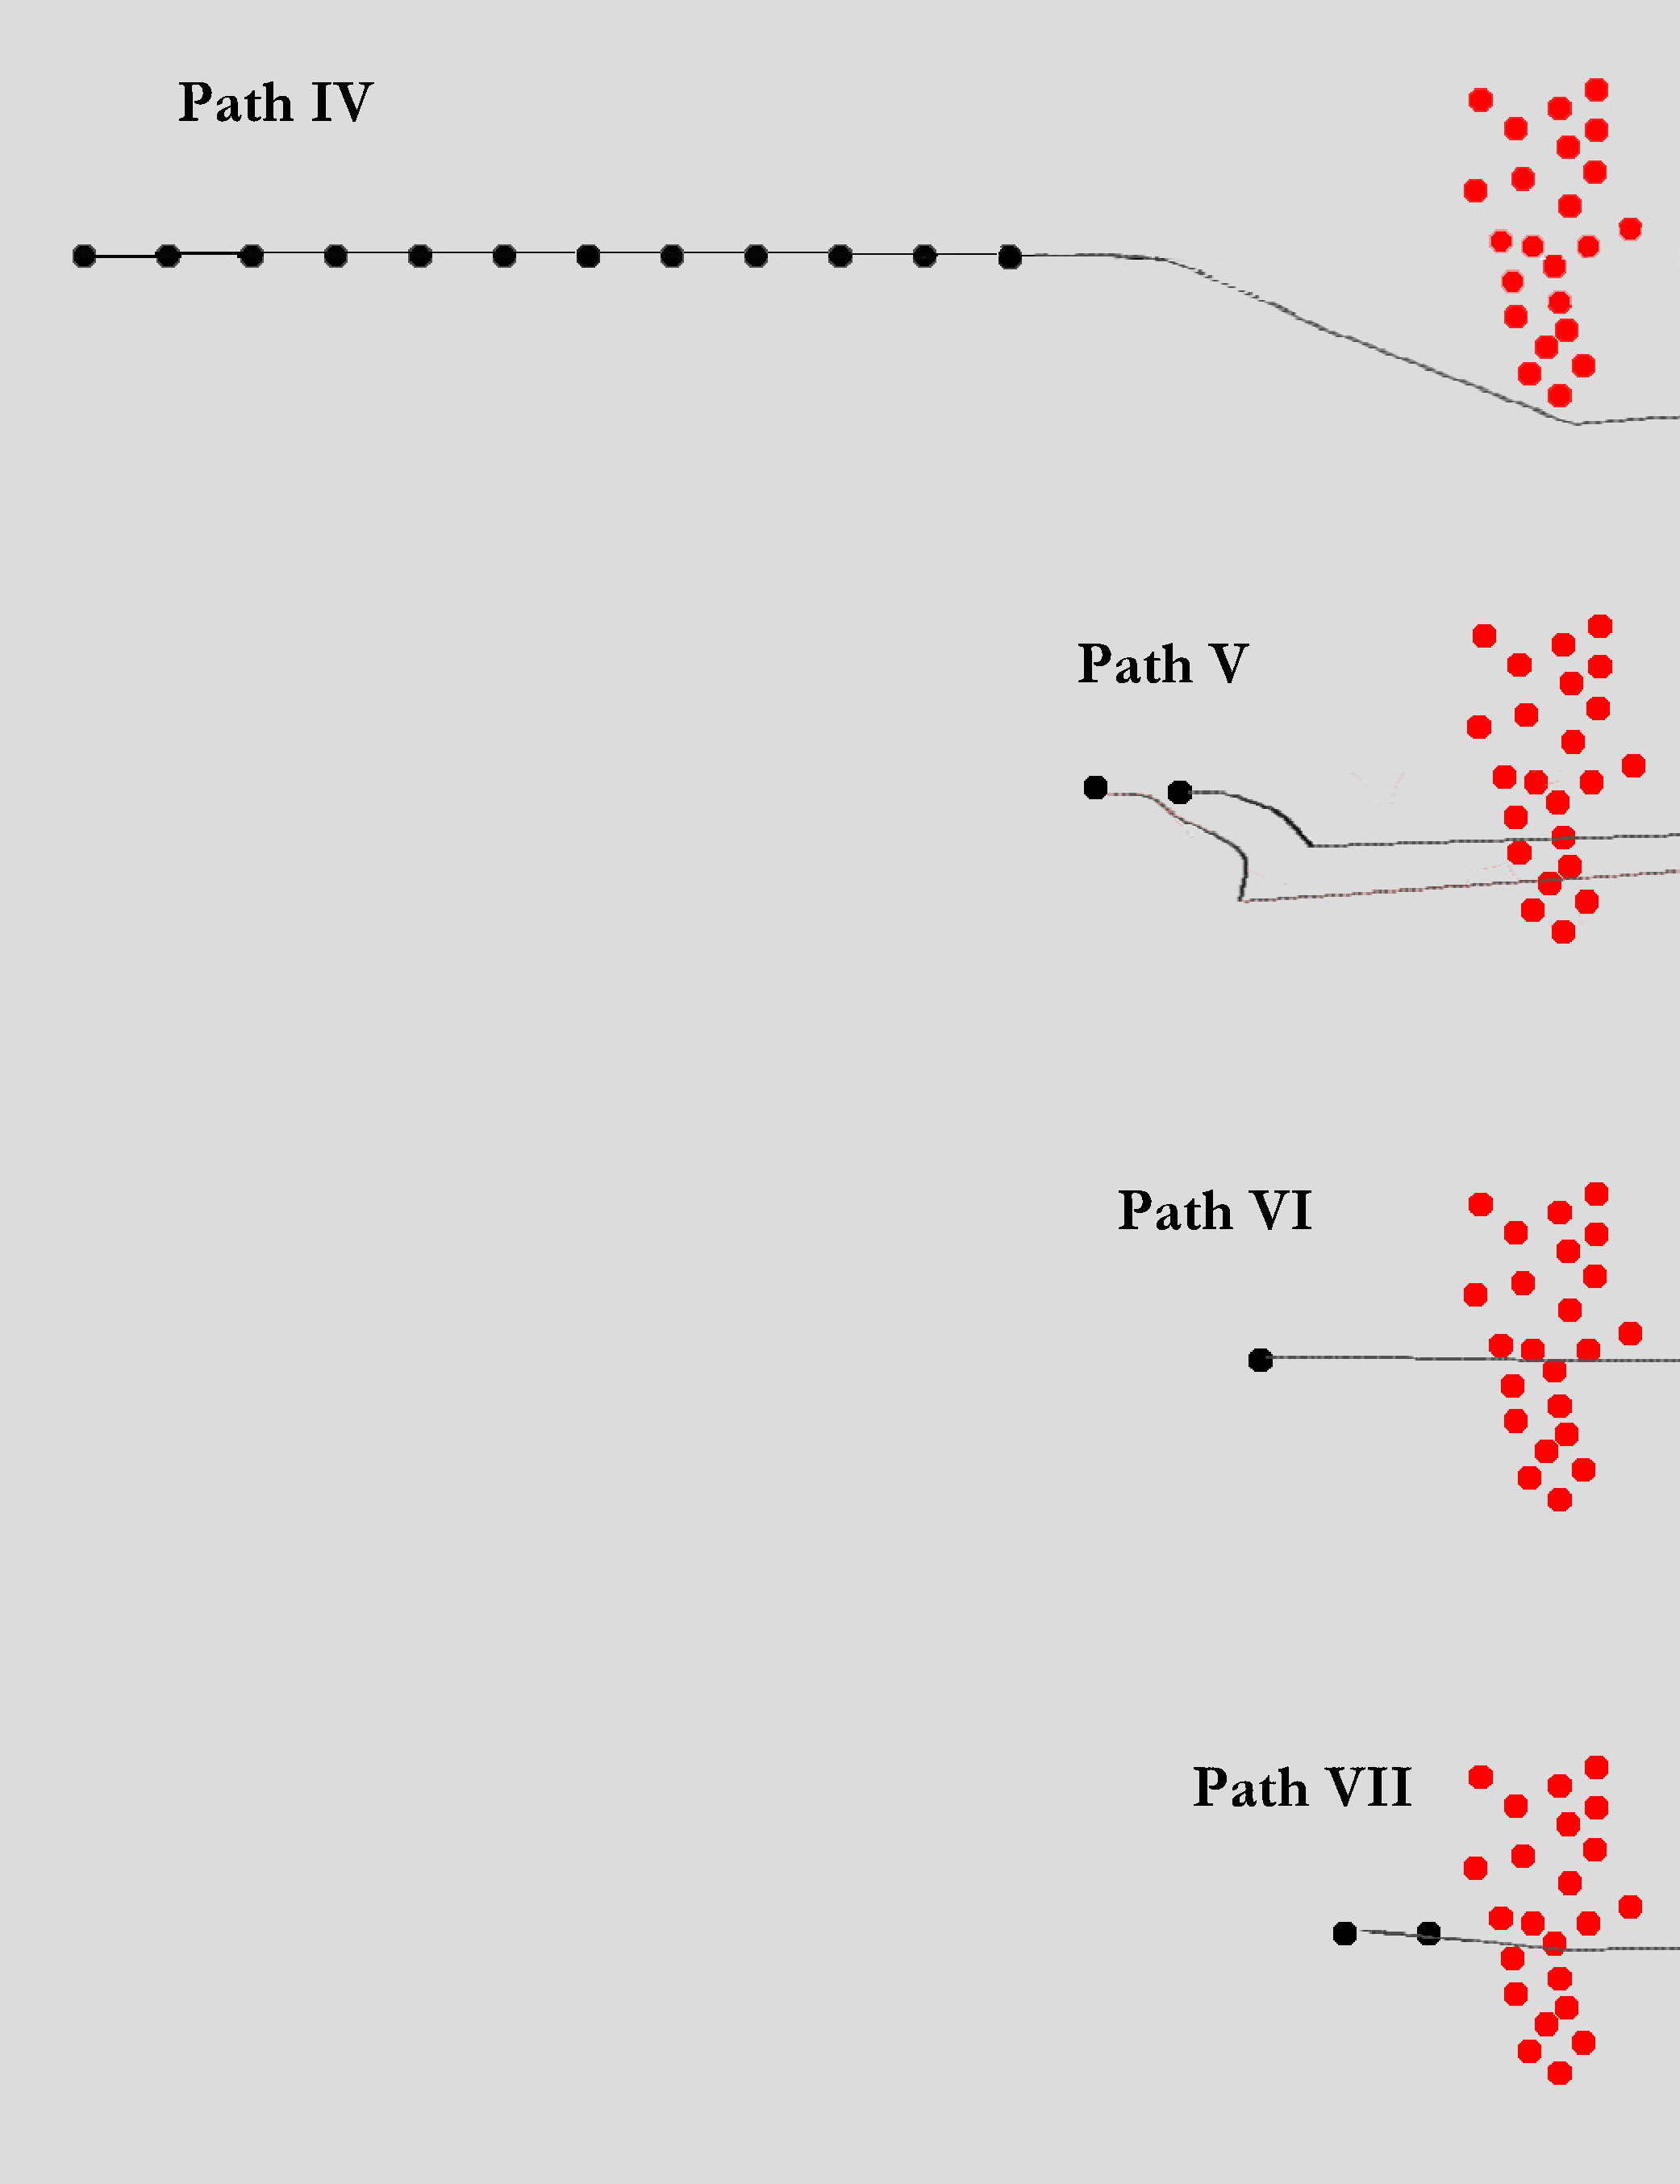
\includegraphics[width=7.5cm,height=12cm]{Exp2_GBP}}
  \caption{Experiment 2: Effect of multi layered clustering}
  \label{Exp2}
\end{figure}

In this experiment, the simple scenario where a single (black) agent had to get past a big group of agents to get to its goal is studied. The same experiment was performed by keeping the agent at different distances from the group. The objective of this experiment is two-fold. Firstly, it demonstrates the importance and the working of the multi-layered clustering (Sect.~\ref{IBP:Sensing}) used. Secondly, it demonstrates that when agents are very close to each other, where RVO2 already performs well, the Group Based Perception does not interfere with RVO2's functioning.

To recap, the multiple layers are used to describe groups of varying size at varying ranges of perception. This means agents will perceive other agents as groups or individuals depending on the distance; as an agent moves towards a group it will start to perceive the group as individual agents.

When GBP isn't used, the path followed does not change significantly with distance. The agents in the path of the black agent, give way to the agent, and the black agent just proceeds straight through the center of the large group (Path I in Fig.~\ref{Exp2_RVO}). In the last few cases (Paths II and III), the path is slightly different because the black agent does not have enough time to plan for a smooth, straight path and hence there is a slight deviation. Also, similar to the experiment in Sect.~\ref{GBP} it is forced to slow down in the process.

The result produced when GBP is used is more varied. Four distinctly different paths (labeled IV, V, VI and VII in Fig.~\ref{Exp2_GBP}) are produced based on how far the oncoming black agent is from the big group. At distances between 7-18m away from the center of the big cluster, the agent has enough time to perceive the group and avoid it completely (Path IV). At distances between 5-7m away, due to the size of the group, the agent gets too close to the group such that it then perceives the group as individuals. At this time (as described in Fig.~\ref{fig:ClusterLayer}) the agent performs motion planning on all the individual agents and as a consequence moves through the group, shown by path V. Path VI is obtained in a similar fashion; however, the black agent is too close to the group (4m away) to discern the effect of GBP. At distances closer than this (2-3m away), the path followed by the agent (Path VII) is exactly the same as that followed by the agent not using Group Based Perception (Path III). We argue that this type of flexibility in the perception of groups is critical to creating more natural behavior, humans will adapt what they perceive based on success or failure of their attempt to avoid larger groups.

\begin{figure}[!t]
  \centering
   \subfloat[Black Agent- Effort]{\label{Exp2_Black_Effort}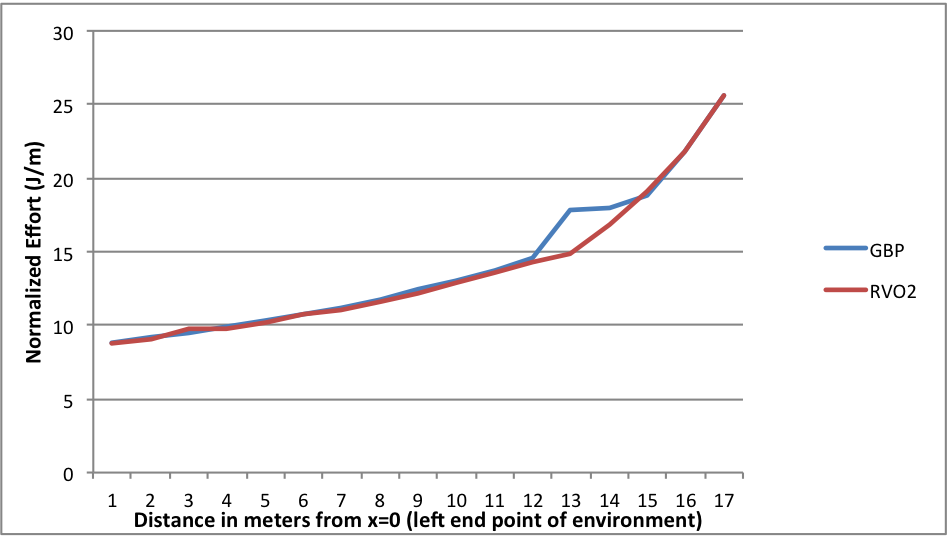
\includegraphics[width=7.5cm,height=5cm]{Exp2_Black_Effort}}
  \hspace{1pt}
    \subfloat[Black Agent- Inconvenience]{\label{Exp2_Black_Inconvenience}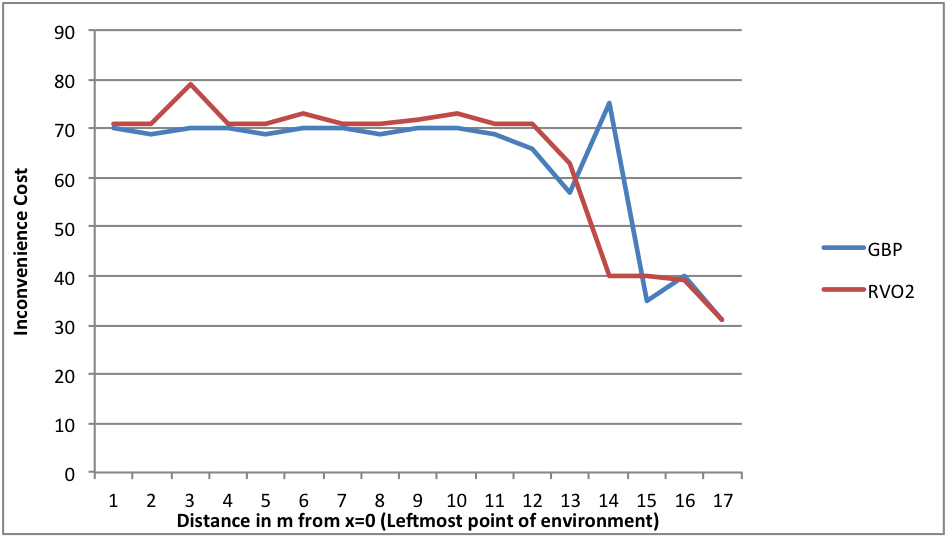
\includegraphics[width=7.5cm,height=5cm]{Exp2_Black_Inconvenience}}
  \\
  \subfloat[Remaining Agents- Effort]{\label{Exp2_Remaining_Effort}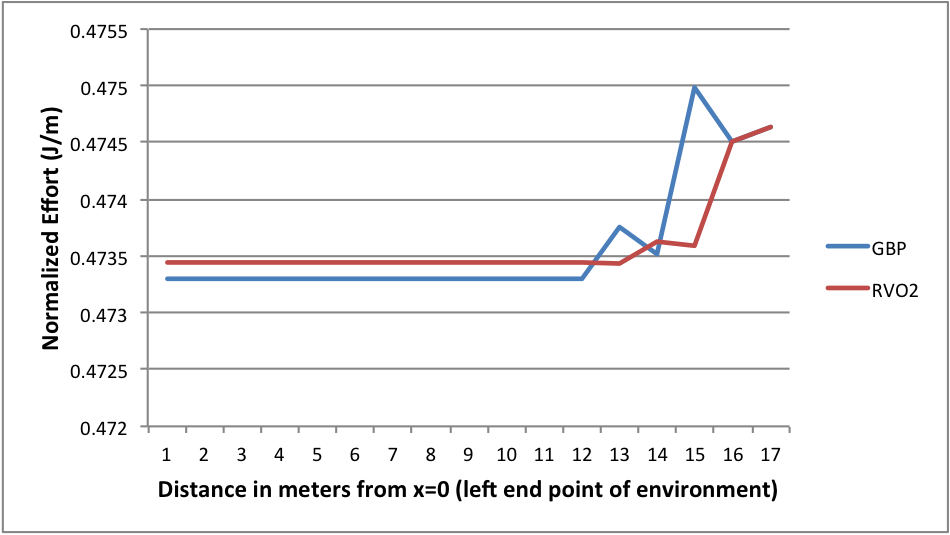
\includegraphics[width=7.5cm,height=5cm]{Exp2_Remaining_Effort}}
  \hspace{1pt}
  \subfloat[Remaining Agents- Inconvenience]{\label{Exp2_Remaining_Inconvenience}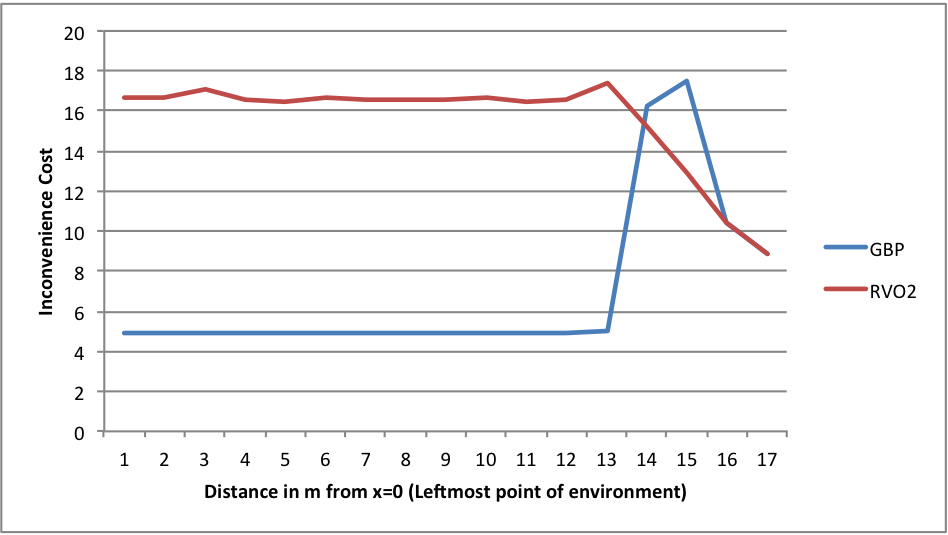
\includegraphics[width=7.5cm,height=5cm]{Exp2_Remaining_Inconvenience}}
  \caption{Experiment 2: Quantitative Analysis}
  \label{Exp2_QuantitativeAnalysis}
\end{figure}

Figures~\ref{Exp2_Black_Effort} and \ref{Exp2_Remaining_Effort} show a comparison of the effort expended by the black agent and the average effort expended by all the remaining agents while using a traditional sensor range and GBP. As in the previous experiment (Sect.~\ref{GBP}) there is hardly any difference in the effort expended in both scenarios (except for a slight increase for path V). However, an interesting pattern can be observed in the inconvenience measurement (Figures Figures~\ref{Exp2_Black_Inconvenience} and \ref{Exp2_Remaining_Inconvenience}). Firstly, the inconvenience for the rest of the group, is always lesser when GBP is used and almost the same for the black agent when path IV is followed. However, when path V or VI is followed there is a spike in the inconvenience curve. This can be explained by considering the fact that in both path V and VI, the black agent changes its planned path suddenly and decides to go through the group, thus not only increasing its own inconvenience but also the inconvenience caused to others in the group who have to move to give way to the agent. Finally, when path VII is followed both the effort and inconvenience count are exactly the same as for path III.

\subsection{Filtering necessitates Group Based Perception}


\begin{figure}[!t]
  \centering
  \subfloat[Initial Scenario]{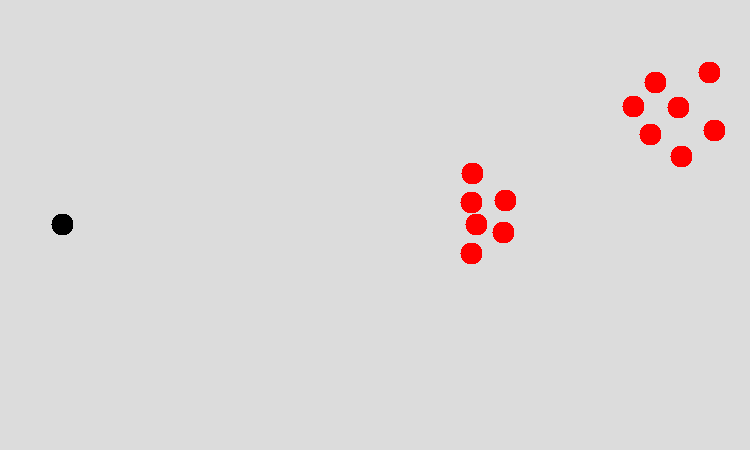
\includegraphics[height=5cm]{Exp3_initial}}
   \\
    \subfloat[Info limit of 4, without GBP]{\label{Exp3_4_RVO}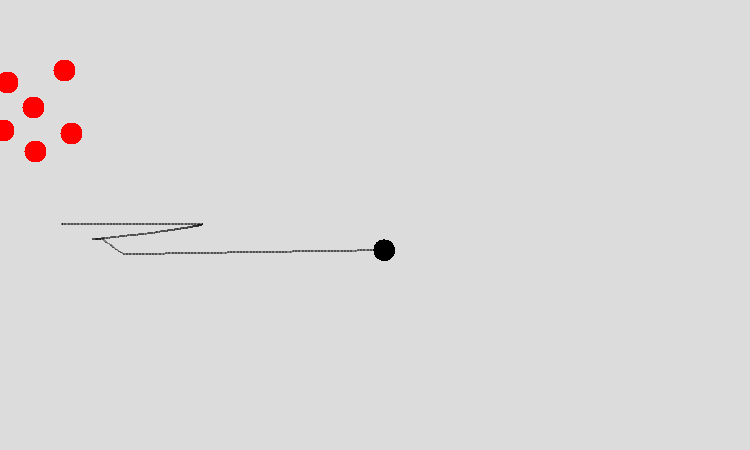
\includegraphics[width=7.5cm,height=4cm]{Exp3_4_RVO}}
    \hspace{1pt}
   \subfloat[Complete knowledge, without GBP]{\label{Exp3_full_RVO}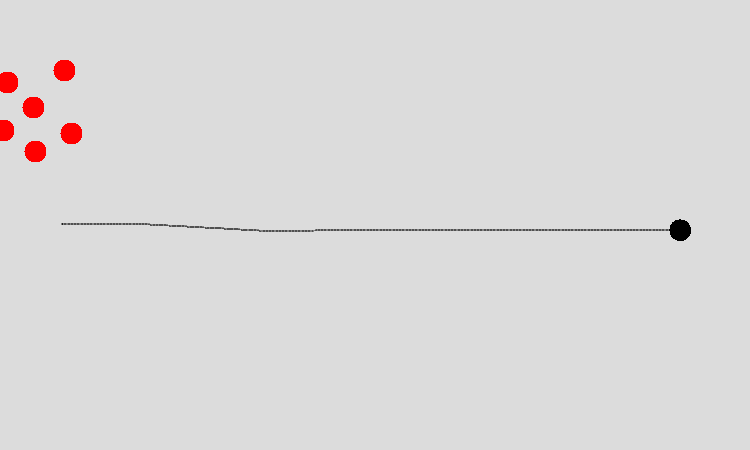
\includegraphics[width=7.5cm,height=4cm]{Exp3_full_RVO}}
  \\
  \subfloat[Info limit of 1, with GBP]{\label{Exp3_1_GBP}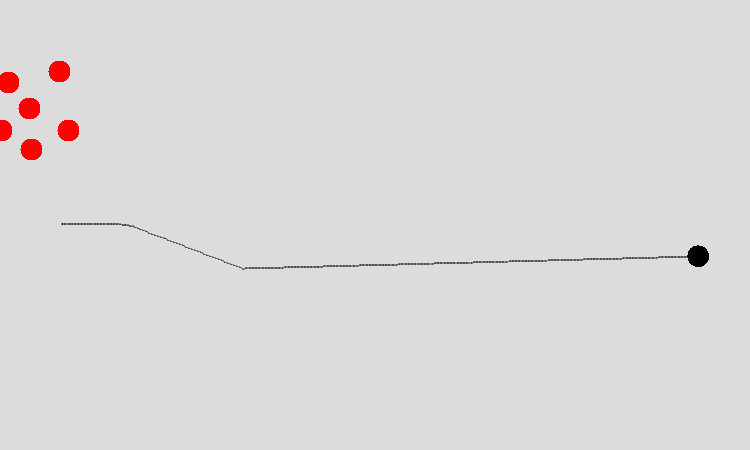
\includegraphics[width=7.5cm,height=4cm]{Exp3_1_GBP}}
  \hspace{1pt}
  \subfloat[Info limit of 4, with GBP]{\label{Exp3_4_GBP}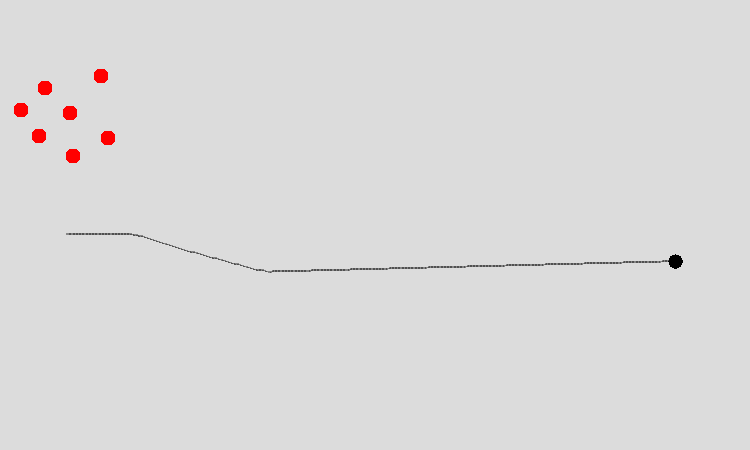
\includegraphics[width=7.5cm,height=4cm]{Exp3_4_GBP}}
  \caption{Experiment 3: The necessity of Group Based Perception}
  \label{Exp3}
\end{figure}

In Sects.~\ref{IBP:Theory}, the fact that humans have limited information processing capacity was explained. In this experiment, it is demonstrated that if a human being's limited information processing capability is to be modeled, it is necessary to use Group Based Perception. This is done by observing the simple scenario of an agent moving towards two groups of other agents (Fig.~\ref{Exp3}). When no information limit is imposed on the agent, and a normal circular sensor range is used, the agent, as expected, follows a nice straight path through the center of the group. However, when an information limit of $a_{IL} = 4$ is imposed on the agent, the black agent, does not perceive all the individual agents in the group and  as a result it is forced to reconsider its path mid-route. As a result, the irregular trail shown in Fig.~\ref{Exp3_4_RVO} is obtained. However, in the same situation, when Group Based Perception is used, the agent smoothly avoids the whole group (Fig.~\ref{Exp3_4_GBP}). In fact, this smooth path is obtained for as low a limit as $a_{IL} = 1$ (Fig.~\ref{Exp3_1_GBP}).

\subsection{Effect of filtering of percept information}

\begin{figure}[!tb]
  \centering
   \subfloat[Initial Scenario]{
\includegraphics[height=5cm]{Exp4_initial}}
   \\
   \subfloat[InfoLimit 3: Step 1]{\label{Exp4_3_1}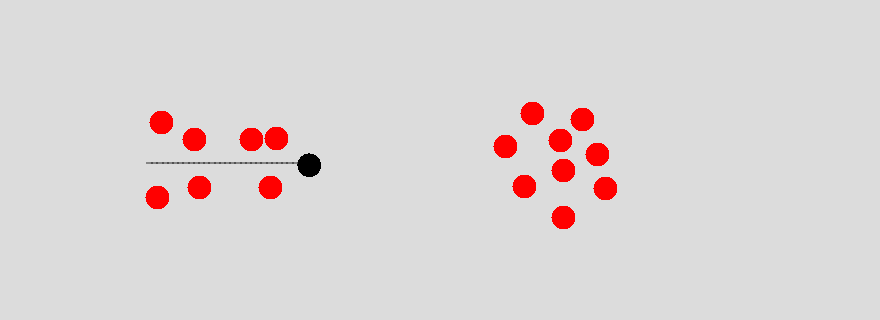
\includegraphics[width=7.5cm,height=4cm]{Exp4_3_1}}
  \hspace{1pt}
    \subfloat[InfoLimit 5: Step 1]{\label{Exp4_5_1}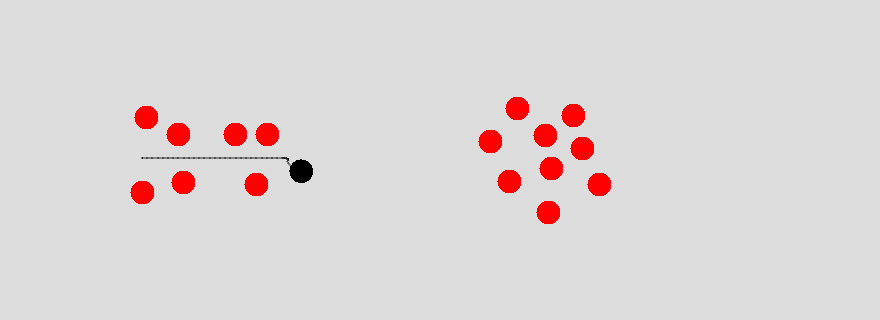
\includegraphics[width=7.5cm,height=4cm]{Exp4_5_1}}
  \\
  \subfloat[InfoLimit 3: Step 2]{\label{Exp4_3_2}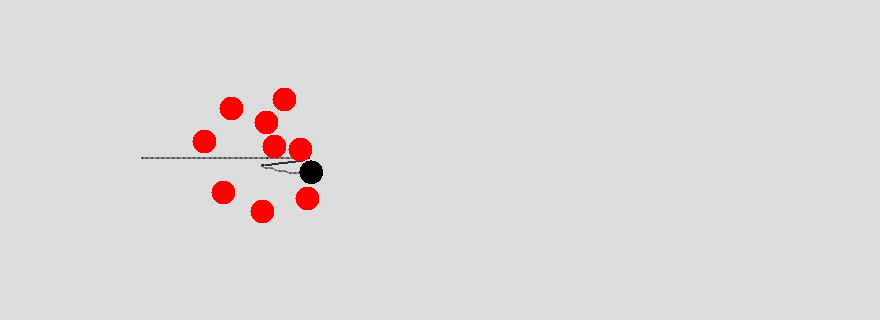
\includegraphics[width=7.5cm,height=4cm]{Exp4_3_2}}
  \hspace{1pt}
  \subfloat[InfoLimit 5: Step 2]{\label{Exp4_5_2}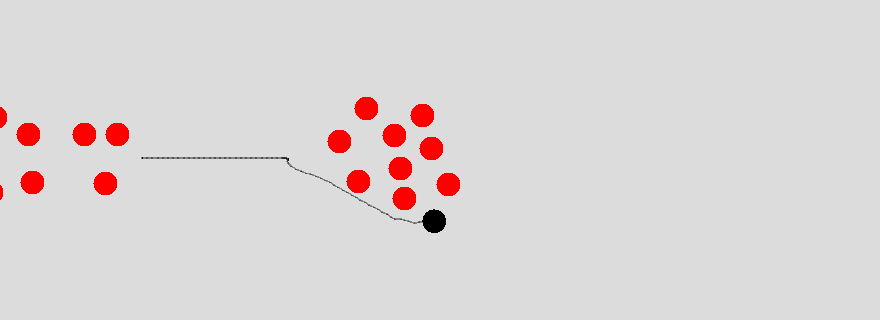
\includegraphics[width=7.5cm,height=4cm]{Exp4_5_2}}
  \caption{Experiment 4: Effect of filtering of percept information}
  \label{Exp4}
\end{figure}

The final experiment (Fig.~\ref{Exp4}) demonstrates the effect of filtering, i.e.\ having limits on the information processing capabilities of the agents. The scenario consists of an agent moving towards a collection of individuals (moving towards the agent) followed by a group of agents behind the set of individuals. In the first case an information limit of $a_{IL} = 5$ is set so that the agent is continually capable of perceiving a larger number of other agents and groups. In the second scenario a lower limit of $a_{IL} = 3$ is used such that the agent isn't initially capable of perceiving the group behind the individuals. Figure~\ref{Exp4_5_1} shows how agents perceive the cluster that is farther away, even when there is an immediate collision to avoid. Figure~\ref{Exp4_5_2} shows that the agent manages to move around this group because it had a head start in planning - i.e.\ , it considered the group early when avoiding collisions. In the second scenario it could process a maximum of 3 or 4 percepts at any given time because of the lower information limit. Due to this, as seen in Fig.~\ref{Exp4_3_1}, the agent cannot see beyond the immediate obstacles in front and does not prepare in advance to avoid the larger group. Once the agent finally perceives this group, it is too late to move around this group as it perceives the group as individuals and then moves through the group as in Fig~\ref{Exp4_3_2}.

This experiment illustrates how small differences in the information limit can generate different forms of behavior in the agents. Interestingly, the info limit of 3 and 5 correspond to Cowan's finding~\cite{Cowan:2001wi} that all humans can cognitively process only 3-5 chunks of information at any given time. Clearly the value of the limit is critical to behavior, it is also proposed that this limit will change with personal characteristics and the emotional state of the agents. In fact this varying limit of perception may be an important factor for collisions in actual crowds, this is especially relevant in emergency egress scenarios where stress and collisions are critically important to safety planning. We plan to attempt to quantify this information limit through experimentation in future work.

\section{Summary and Future Work}
\label{IBP:Conclusion}
In this chapter, the Information Based Perception model for agents which is based on perceived information rather than spatial distance has been introduced. The argument that this is a more appropriate model of human perception for crowd and egress simulation has been made. The behavior of this system has been illustrated through experiments. It has been shown and argued that this creates more realistic group avoidance behavior. The idea that humans have limited perception capacity such that they only process certain obstacles more relevant to collision avoidance is incorporated; this in turn will result in a reduction in efficiency of collision avoidance.

As mentioned earlier, for the IBEVAC model, the IBP model will have to be extended so that during filtering it can recognize cues that contain event and environment information and pass it to the appropriate modules for processing. Also, critical to the model is the quantification of information limits and appropriate definitions of interest; real world experiments will be conducted to attempt to quantify these parameters. The third criteria which was mentioned in Sect.~\ref{IBP:Filtering}, i.e.\ the inherent interestingness of the object, will also be the subject of these real world experiments. In emergency situations, according to Ozel~\cite{Ozel:2001tn}, humans start perceiving cues in the environment differently. This idea was touched upon in the literature review chapter. The idea of modeling different cues and their effect on the agent's information processing capabilities as suggested by Kuligowski~\cite{Kuligowski:2009un} is an idea that will be discussed in more detail in Chapter~\ref{chapter:ConclusionAndFutureWork}. As mentioned by Hill~\cite{Hill:1999ww} there is also a reciprocal effect of cognition on perception where agents would turn towards objects of more interest. It is planned that this will also be incorporated into later version of the IBP model. The next chapter concludes this report by giving a brief description of the other parts in the model that have been considered so far and a more complete description of how the final IBEVAC model will look.



    %!TEX root = thesis.tex

\chapter{Modelling Pre Evacuation Behavior in Agent Based Simulations Of Crowds}
\label{chapter:PreEvacuationBehavior}

\section{Introduction}
\label{intro}
Ideally, when a fire starts a fire alarm goes off; all occupants hear this alarm and use the nearest safe exit to leave the building. However, this is hardly the norm. In many cases, occupants are desensitized from hearing false alarms and often do not start to evacuate until they are completely sure that it is needed. On January 19, 2000, a fire in Boland Hall in Seton Hall University killed three students because they had ignored the fire alarms assuming they were false~\cite{Berry:2000us}. This uncertainty about the authenticity of the first sign of danger isn't an isolated incident~\cite{Proulx:2003tc,Purser:2001ts,Tong:1985wn}. Hence, when studying the behavior of evacuees, it is necessary to study and understand their actions from the time at which the fire started right up until the point where the last person evacuated~\cite{Tong:1985wn}. Modeling and simulation is one approach for analyzing and understanding egress behavior.

Software that simulates crowd egress is necessarily very complex because crowd egress from a building is itself a very complex system with lots of interacting elements (people, fire, alarms, etc.) each of which can cause different complications in the system. One of the most popular methods for studying and modeling complex systems is through Agent Based Models (ABM). In ABM, a set of heterogeneous, intelligent entities called agents are programmed with behavior approximating humans and placed in a partially observable environment. Asynchronous interactions between agents result in macro-level dynamics which can help observers learn more about the system.

Pre-evacuation uncertainty and investigation are features of human behavior during egress that are rarely considered in models. Pre-evacuation refers to the period of time that elapses after the start of the fire alarm before the person starts evacuating. While some models~\cite{Tsai:2011tz} do have a simplified model of pre-evacuation behavior, they fail to model it in enough detail to enable their extension to more general cases. For example, a fire alarm could have different effects based on the clarity and believability of the alarm~\cite{Kobes:2009jx,Paulsen:1984ti}. This variability is hard to model in existing models of pre-evacuation behavior. Also, during an evacuation people exchange event and environment related information with other evacuees. Evacuees are unlikely to follow blindly any and all messages that they receive. There is a variability in the \emph{trust} in messages received that can have different effects on egress. This is rarely considered in existing models.


In this paper, we present one aspect of a behavioral model for Agent Based Modeling of crowd egress which we call the IBEVAC (Information Based Evacuation) model. This behavioral model models evacuees as information processing entities. More specifically, in this paper we introduce the information-based event identification and communication system that is used in IBEVAC. The evacuees identify and process information in terms of event cues which exist throughout the environment. The importance of modeling pre-evacuation behavior and a communication system is illustrated through experimentation.

\section{Related Work}
\label{LitRev}


A fire evacuation is a complex situation to model and simulate. One large component of this complexity is the need to understand the behavior and decision making of the people taking part in it. There are a lot of conflicting theories on how humans behave in emergencies and why they behave as they do. However, there are also certain parts of human nature that are generally accepted to be true, such as the constant search for information~\cite{Proulx:2003tc,Tong:1985wn,Ozel:2001tn,Sime:1983uy}. This section first summarizes the existing knowledge of human behavior during egress with special emphasis on pre-evacuation behavior. Following this, some existing models of pre-evacuation behavior and communication is presented.

\subsection{Pre-evacuation Behavior}
\label{PreEvacuationBehavior}

Several studies of human behavior during emergency egress~\cite{Kuligowski:2005tt,Ozel:2001tn,Proulx:2007ul}, have shown that an evacuee's first reaction after realizing that there is an unusual situation is to investigate and gather more information about the situation. Evacuation starts only once the need for evacuation is established. \emph{Cues} are the key to understanding this transition from realization to investigation and, eventually, to evacuation. Cues are certain changes in the environment that indicate that something is wrong or different from normal~\cite{Sime:1983uy}. They come in a variety of different forms. Fire and smoke are the typical and most unambiguous cues for an evacuation. Fire alarms and people running about are examples of more ambiguous cues. According to Proulx~\cite{Proulx:2007ul}, an ambiguous cue by itself does not cause a person to initiate investigation. Rather, the cue has to persist for a period of time before investigation begins.

There have been several surveys, interviews and other studies of the factors that influence evacuation and pre-evacuation behavior. Kuligowski~\cite{Kuligowski:2009un} summarized the key findings of these studies and compiled a list of factors that influence pre-evacuation behavior. She suggested that the period that we term as pre-evacuation itself consists of two phases. Phase 1 is called \emph{perception}. This refers to the perception of some unusualness in the current situation. Kuligowski calls the next phase \emph{interpretation}. During this phase, the person searches for more information to verify whether a fire has actually started and if it actually poses a threat that needs to be handled. Several others~\cite{Ozel:2001tn,Proulx:2007ul,Tong:1985wn} have also emphasised the importance of this phase though sometimes under different names. Regardless of what it is called, this phase consists of two parts~(1) defining the situation as a fire and~(2) defining the risk that the situation poses.

% Explaing milling somewhere here.

Kuligowski categorized the factors that influence these phases into two types: occupant based factors and cue based factors. Occupant based factors are intrinsic characteristics of the evacuee like age, experience, gender, etc. One of the factors that encourage the programmatic implementation of cue based factors is the fact that the effect of a cue can be explained to be caused by the nature and characteristics of the cue rather than the specific cue. In other words, each cue can be described in terms of its ambiguity, consistency with other cues and its source and it is this description that determines the effect of the cue.


\subsection{Existing models}
\label{ExistingModels}

As mentioned in Section~\ref{intro}, there are very few existing models that take the pre-evacuation period into consideration. Pires~\cite{Pires:2005gs}  modeled the pre-evacuation decision making of an individual using a simple Bayesian Belief Network~(BBN). Fran{\c c}a et al.~\cite{Franca:2009wq} created a simulation model of the development of panic behavior during emergency egress. This model implemented the hysterical belief theory~\cite{Torres:2010tj} and modeled how panic first develops and then evacuation happens. It also had a basic communication system through which agents exchanged mood information (which is a key factor in the development of panic) by using the grid based environment as a medium for communicating messages. Despite pre-evacuation behavior being modeled in some detail, it is not possible to extend this model to replicate the heterogeneity in people's reaction to cues. ESCAPES~\cite{Tsai:2011tz} is a fairly recent model that takes into account some factors like the spread of knowledge, fear and emotion between the different evacuees. These factors are used to create a simplistic model of pre-evacuation behavior. The event identification and communication model proposed in this paper have been influenced by these models but is unique in the way that the diversity of cues and their effects can be considered.

% \section{The IBEVAC Model}
% \label{IBEVAC}


% \begin{figure}[!tb]
% \centering
% 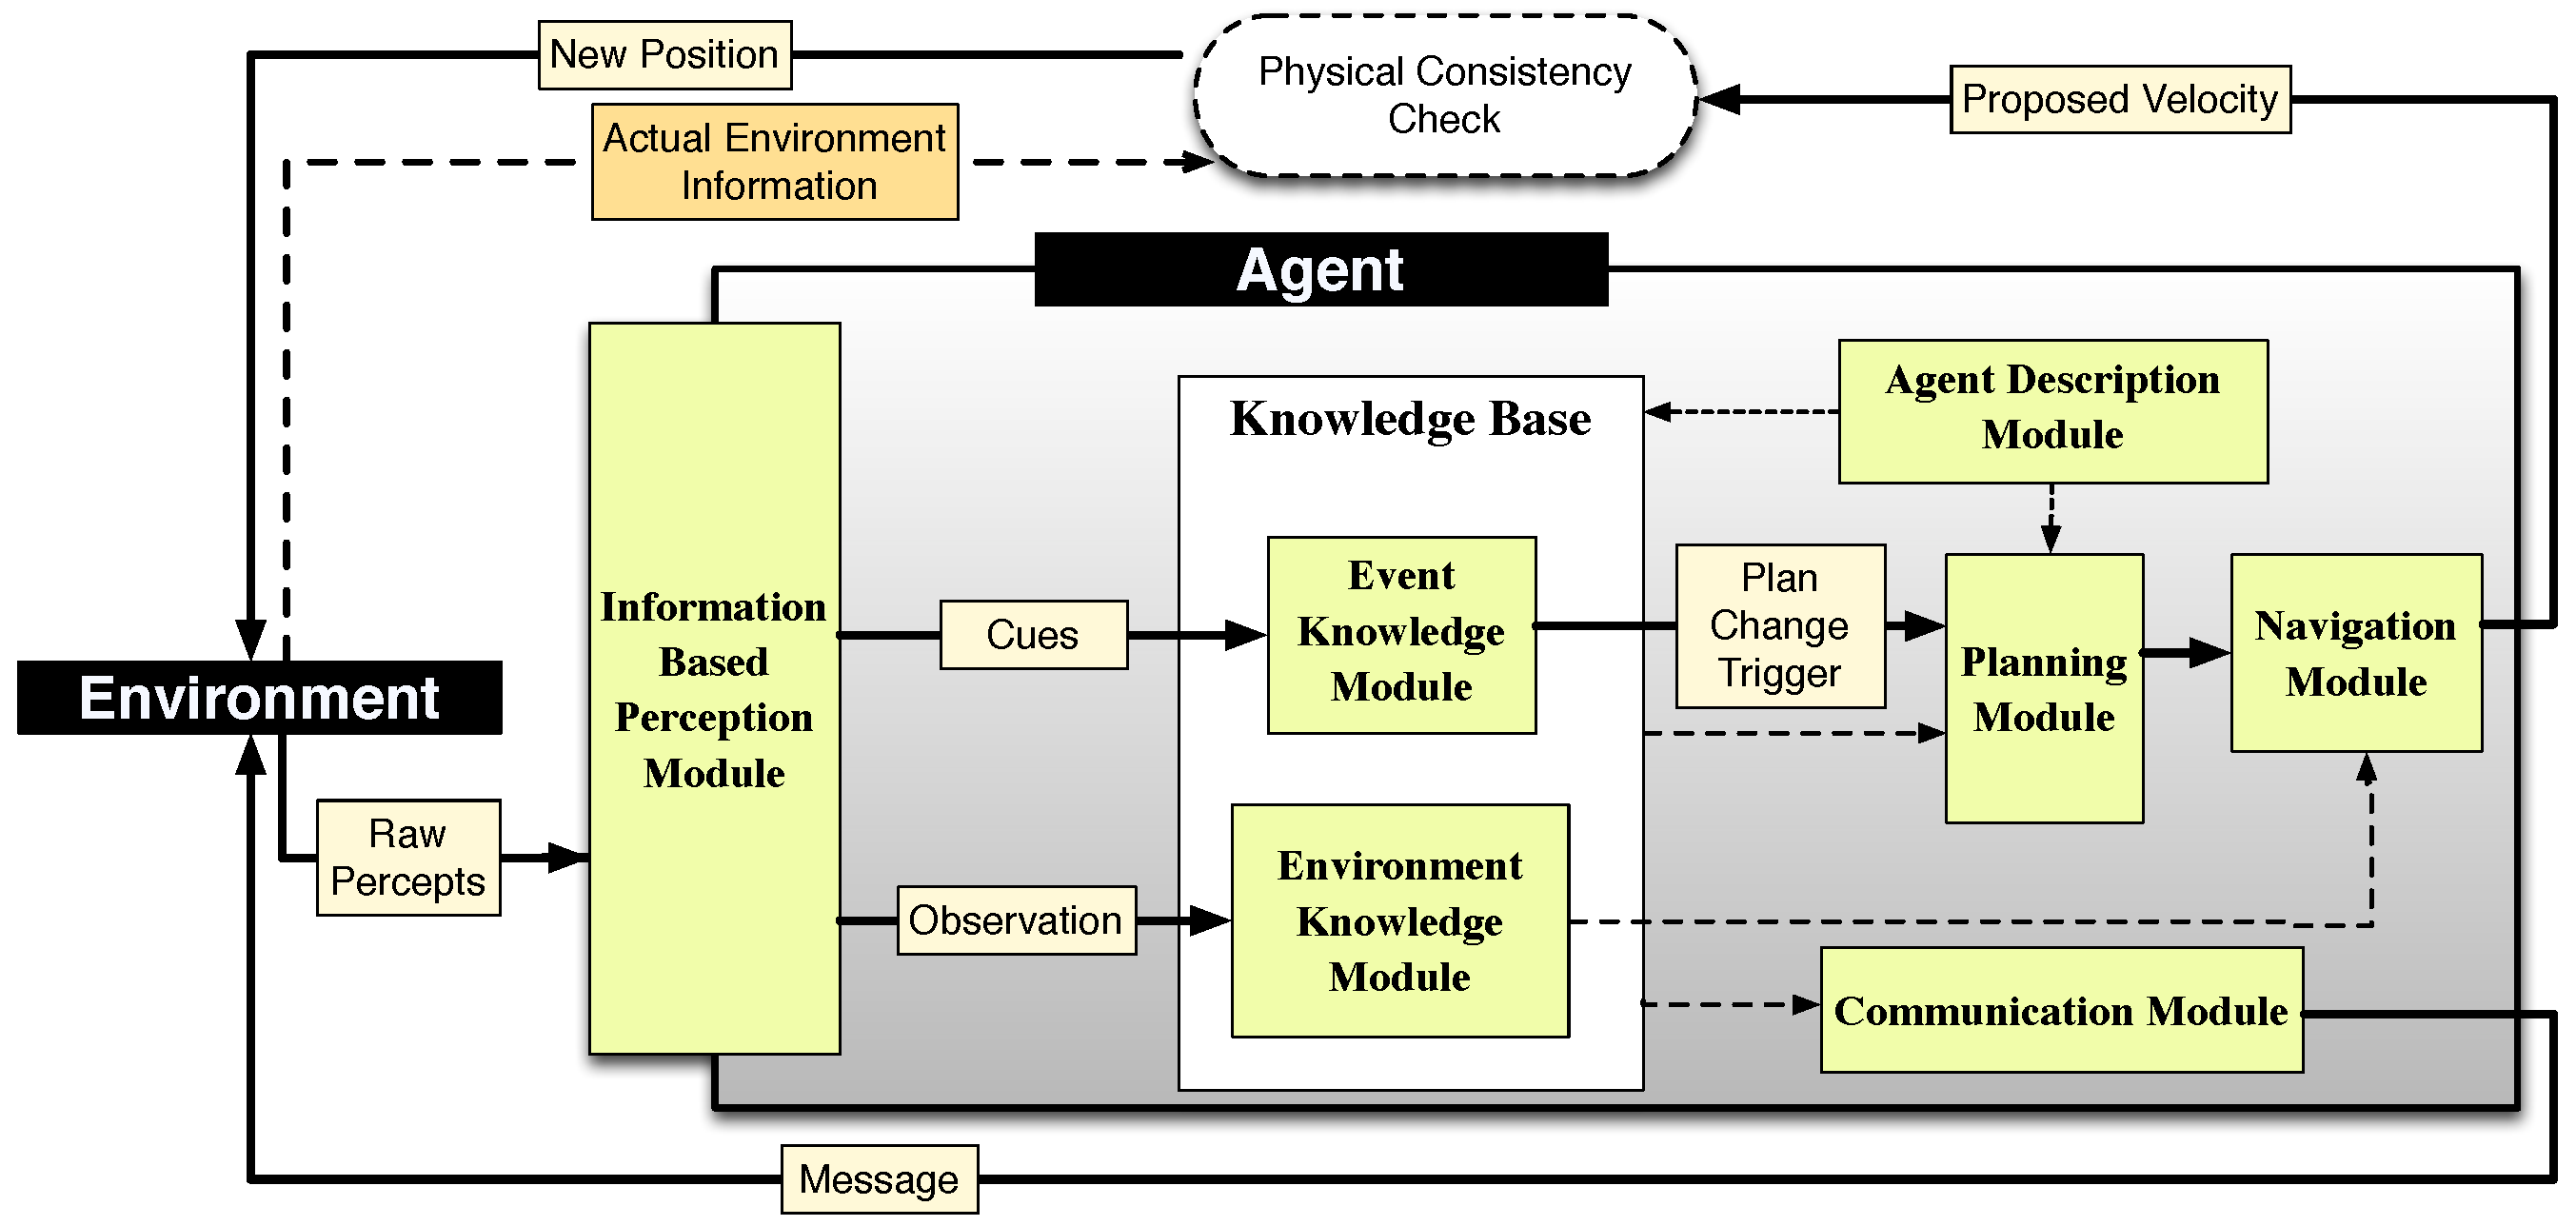
\includegraphics[height=1.9in]{SimplifiedAgentArchitecture}
% \caption[The Agent Architecture]{An illustrated representation of the IBEVAC agent architecture}
% \label{fig:AgentArchitecture}
% \end{figure}

% This section gives an overview of the modular IBEVAC agent architecture. Figure~\ref{fig:AgentArchitecture} shows this architecture. There are many objects or actions that an agent can sense or observe in the environment. We call these \emph{raw percepts}. According to their sources, they can be classified as \emph{observations} from the environment and \emph{messages} from other agents. The Information Based Perception~(IBP) Module is the only gateway through which the agent receives information from the environment. This module is explained in more detail in~\cite{Viswanathan:ut}. The IBP Module passes a percept to the Knowledge Base.

% The \emph{Environment Knowledge Module} stores a representation of the layout of the environment that is formed as a result of the observations of the agent. Information regarding accessibility of links is also stored. As a detailed discussion of this module is beyond the scope of this paper, all agents are assumed to have complete knowledge of the layout. However, agents can learn about inaccessible links only through direct observation or through messages from other agents. The {\em Event Knowledge Module} is the focus of research in this paper. It stores the agent's beliefs about the current state of the environment. Cue perception alters these beliefs and triggers a state change in the agent which is then handled by the Planning Module. This Module is explained in more detail in section~\ref{EventIdentification}.

% The intrinsic characteristics of the agent like the agent's size, speed, mass and social role are stored in the {\em Agent Description Module (ADM)}. It is also responsible for determining the strategies and actions taken by the Planning Module and in determining the effects of the cues on the Event Knowledge Module (Section~\ref{EventIdentification}). The {\em Planning Module} stores the current state of the agent i.e. whether it is exploring, milling or escaping and creates a plan of action for the agent as a set of goals. Each goal is a location that is passed to the Navigation Module.

For the purpose of this paper, three kinds of behavior are modeled: normal behavior where the goal is the center of the \emph{home} room of the agent, for milling behavior the agent gathers with other agents at the nearest \emph{corridor} (See Figure~\ref{fig:layout}) and during escape the agent heads towards the nearest exit.

Communication between agents is facilitated by the {\em Communication Module}. It transmits messages to agents within a communication range. The working of this communication is explained in more detail in Section~\ref{EventIdentification}. The {\em Navigation Module} uses a four level navigation system. At the highest level, a logical path is determined in terms of rooms to be crossed from the agents current location to the goal. From this logical path, spatial way points or locations are extracted by the next level. The third level determines a possible collision free path to the farthest visible spatial way point. Finally, a physics engine ensures that objects don't pass through other objects.

\section{Event Identification and Pre-evacuation Behavior}
\label{EventIdentification}

% First explain how cues are modeled
It is known that the ambiguity, source and consistency of the cue~\cite{Kuligowski:2005tt,Sime:1983uy,Tong:1985wn} are the key factors (Section~\ref{PreEvacuationBehavior}) in determining the effect of a cue. In the IBEVAC model, this is used in modeling all cues in the same way. Each object or event that is to be perceived as a cue implements a \emph{Cue interface} which ensures that each cue can be explained in terms of its ambiguity, source and consistency. This is one of the key novelties of IBEVAC's approach to behavior modeling. Each cue is located at a particular location in the environment and is sensed by agents when within their perception range.

% Next explain how these cues affect the event knowledge module and the idea of buckets and thresholds. One line about how these thresholds are connected to different stages.
Once perceived, these cues are passed to the Event Knowledge Module. The  module has a \emph{bucket} of information corresponding to \emph{uncertainty} and another corresponding to \emph{fire}. When a cue is perceived, appropriate amount of information is added to the appropriate bucket(s) based on the ambiguity level. A less ambiguous cue contributes more information. For each bucket, a \emph{threshold} is initially fixed by the ADM. When the amount of information in a bucket overflows the threshold, a trigger is sent to the Planning Module to change the agent's state and strategy.

% Following this explain how messages contain message cues and additional information.
Communication is implemented as \emph{messages} sent from one agent to the other. Each message has a message cue and environment information. The message cue works just as other cues. Here the term ambiguity is used to refer to the trustworthiness of the source of the information. In this paper, the environment information that is passed is only about the inaccessible paths in the map. % Finally summarize what all happens during a simulation.
During an IBEVAC simulation, a cellular automata based fire model and a simple finite difference smoke model are executed. This creates fire and smoke cues at locations near the fire. As soon as the fire starts, fire alarm cues are placed all over the environment. Agents react to these cues and mark observable pathways that are blocked as inaccessible in their Environment Knowledge Module. All agents either escape or are killed at the end of the simulation.



\section{Results}
\label{Results}

% Outline what are the things that we expect to demonstrate
Experiments were conducted using IBEVAC to demonstrate the effect that cue perception and communication can have on egress. Both experiments were conducted on the two floor office environment shown in Figure~\ref{fig:layout}. Simulations were conducted with 200 agents randomly distributed all over the environment and data was collected after averaging over 100 replications of the simulation.

\begin{figure}[!tb]
\centering
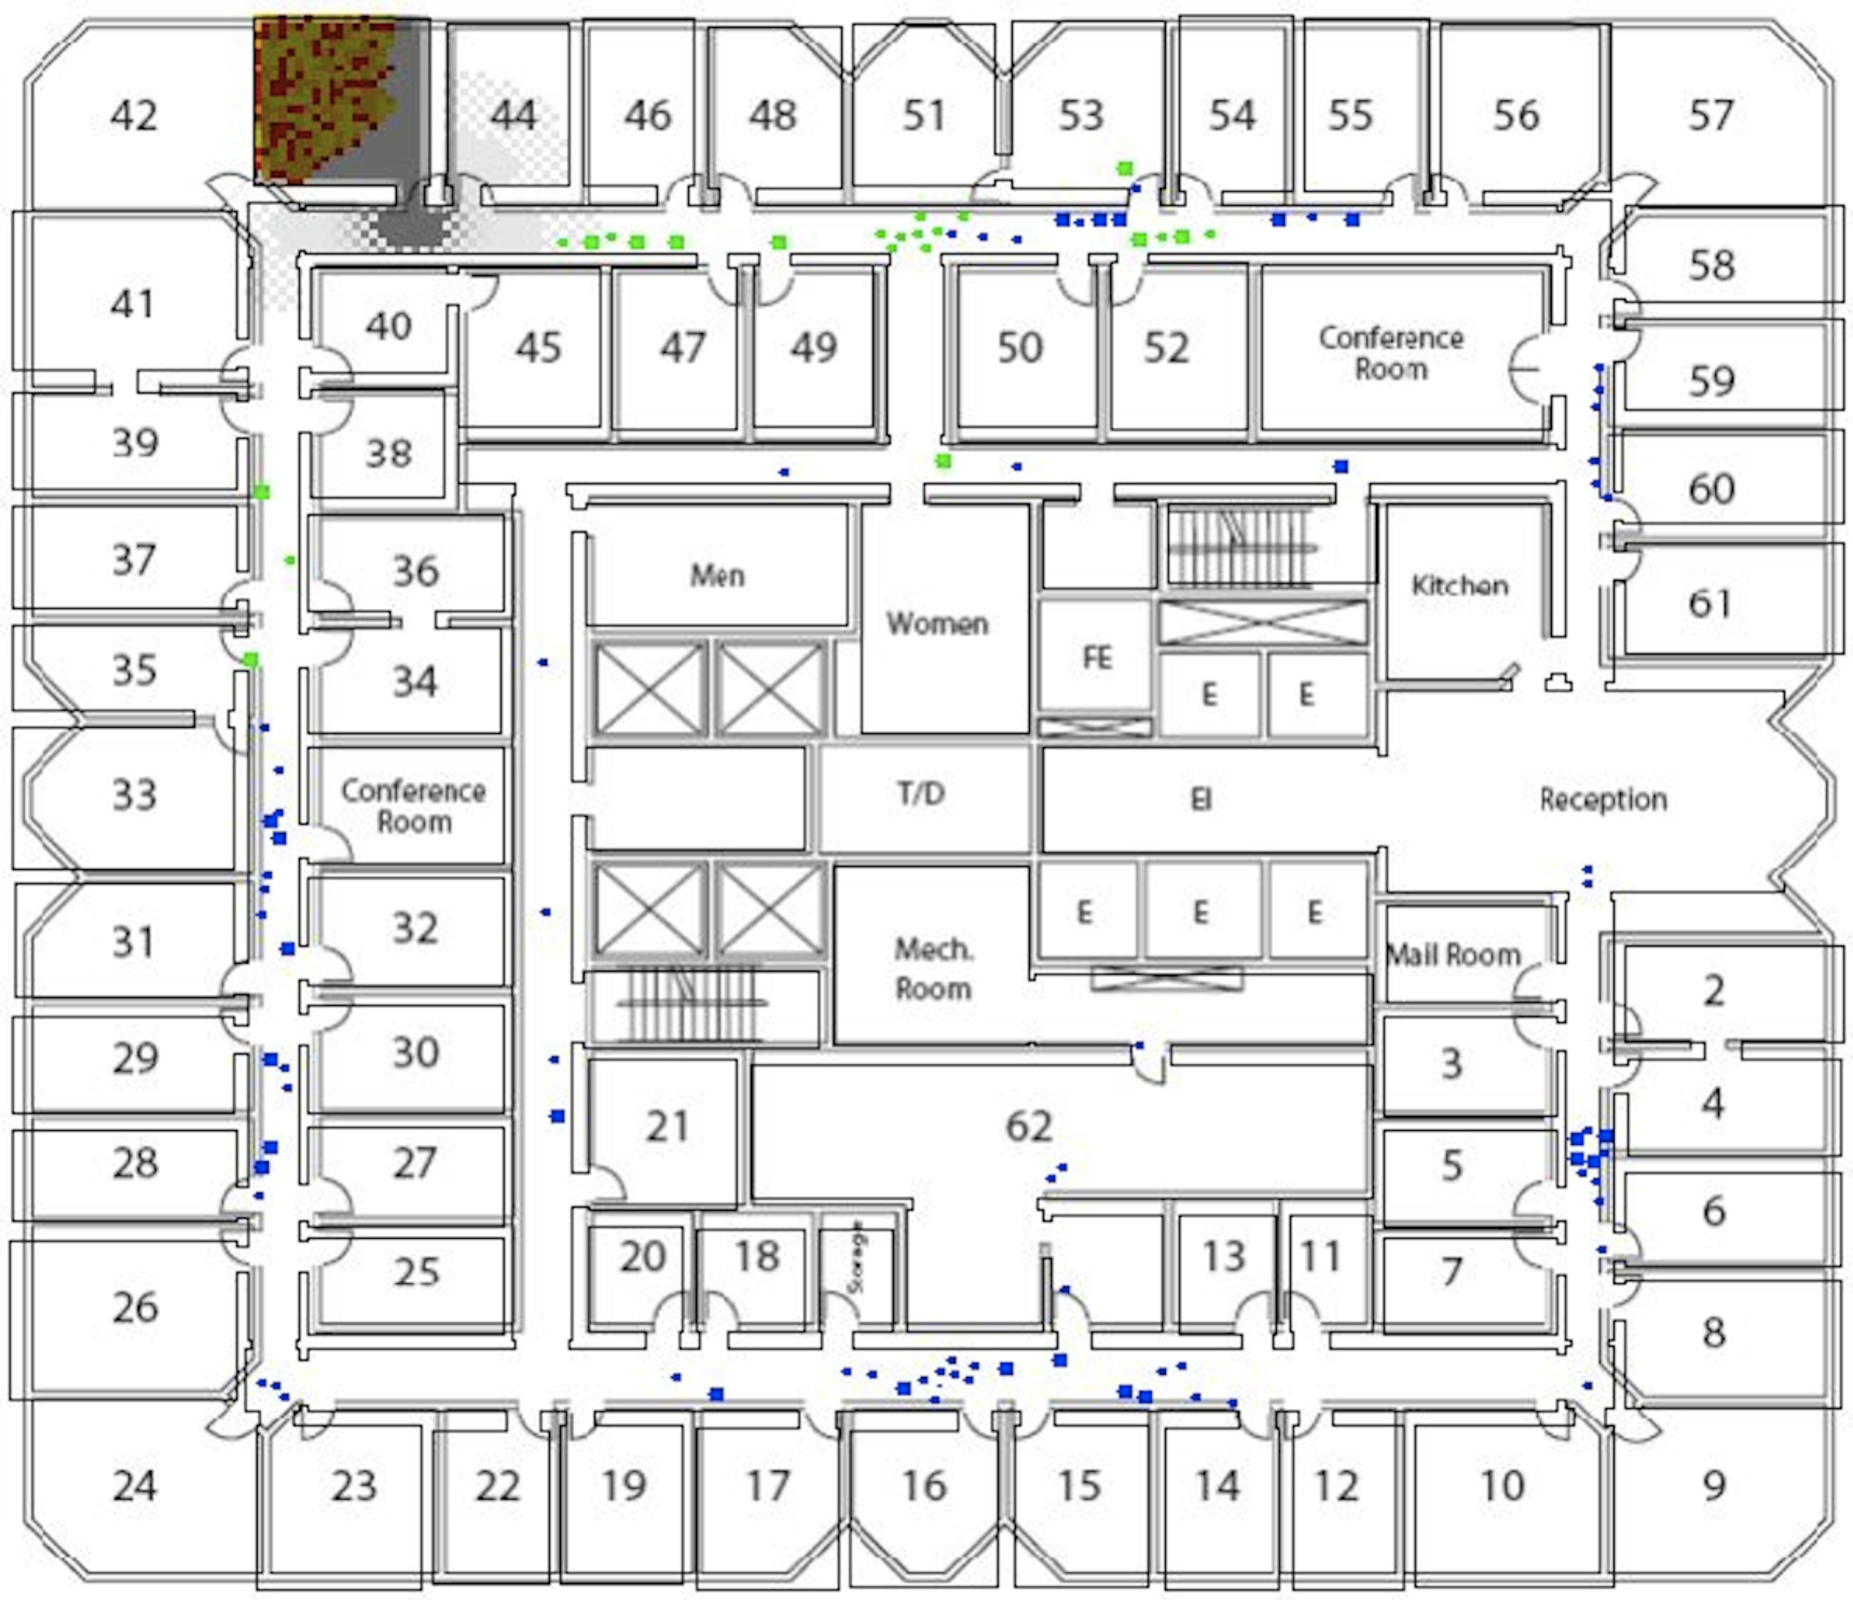
\includegraphics[height= 2.5in]{layout}
\caption[The Environment Layout]{First of two floors from World Trade Center, California. Fire is started in the corner room and generates smoke. Fire kills agents. Smoke depending on concentrations slow or kill agents. The longer rectangles are corridors connecting rooms and the open area on the right center is the exit.}
\label{fig:layout}
% Change to my figure
\end{figure}

% Explain the layout of the environment, the settings and parameters

\subsection{Experiment 1: The effect of fire alarm clarity}
\label{experiment1}

In this experiment, the effect that fire alarm cue clarity and ambiguity has on egress was examined. It is assumed that the fire alarm can be heard clearly at every location on the map; so cues are placed in every room. A fire alarm with a simple ringing sound is much less clear and more ambiguous than a public announcement system that explicitly states that it is not a drill and gives real time updates about the situation. To examine the effect of this difference in clarity, the experiment was repeated for different values of ambiguity (from 0.0 - 1.0). The blue curves in Figure~\ref{Graph1} show the error plot of the survival percentage and the one in Figure~\ref{Graph2} the average time taken for last agent to start evacuating for this experiment. As expected there is a significant drop in number of survivors as the ambiguity of the alarm increases. Also, the later an agent starts evacuating, the lesser is his chance for survival.



% Think about someway to plot the distribution of evacuation start time against ambiguity. This might be a better measure.

\subsection{Experiment 2:  The importance of communication}
\label{experiment2}

In this experiment, the effect of message trustworthiness (ambiguity) is modeled. The fire alarm ambiguity is kept at 1.0 to minimize its interference with the effect of message cues. Similar to experiment 1 the cue ambiguity is varied from 0.0 to 1.0. The green curves in Figure~\ref{Graph1} and Figure~\ref{Graph2} show the results for this experiment. However, both these data are collected for agents in the lower floor only. This is because none of the agents on the higher floor start evacuating as they neither observe the fire nor get a message from other agents about the fire. A similar trend can be observed where the survival rate decreases with increasing ambiguity. The green curve in Figure~\ref{Graph2} flattens out towards the end because in both these cases, the agent's trust in other agents is so less that the only reason they start evacuating is because of the smoke or fire itself. Another thing to note is that even if all agents are completely trusted (ambiguity=0), the last agent still takes a long time to start evacuating because it takes a long time for the information to propagate to it. This can also explain why there is such a dramatic change in the effect of slight change in ambiguity of the fire alarm cue as opposed to a change in ambiguity of the message cue.


%Might it have made more sense to carry this experiment out slighlty differently from the other one in varying the number of high trust and low trust ppl? rather than one unique ambiguity value for all messages?

% \begin{figure}[!tb]
%    \centering
% 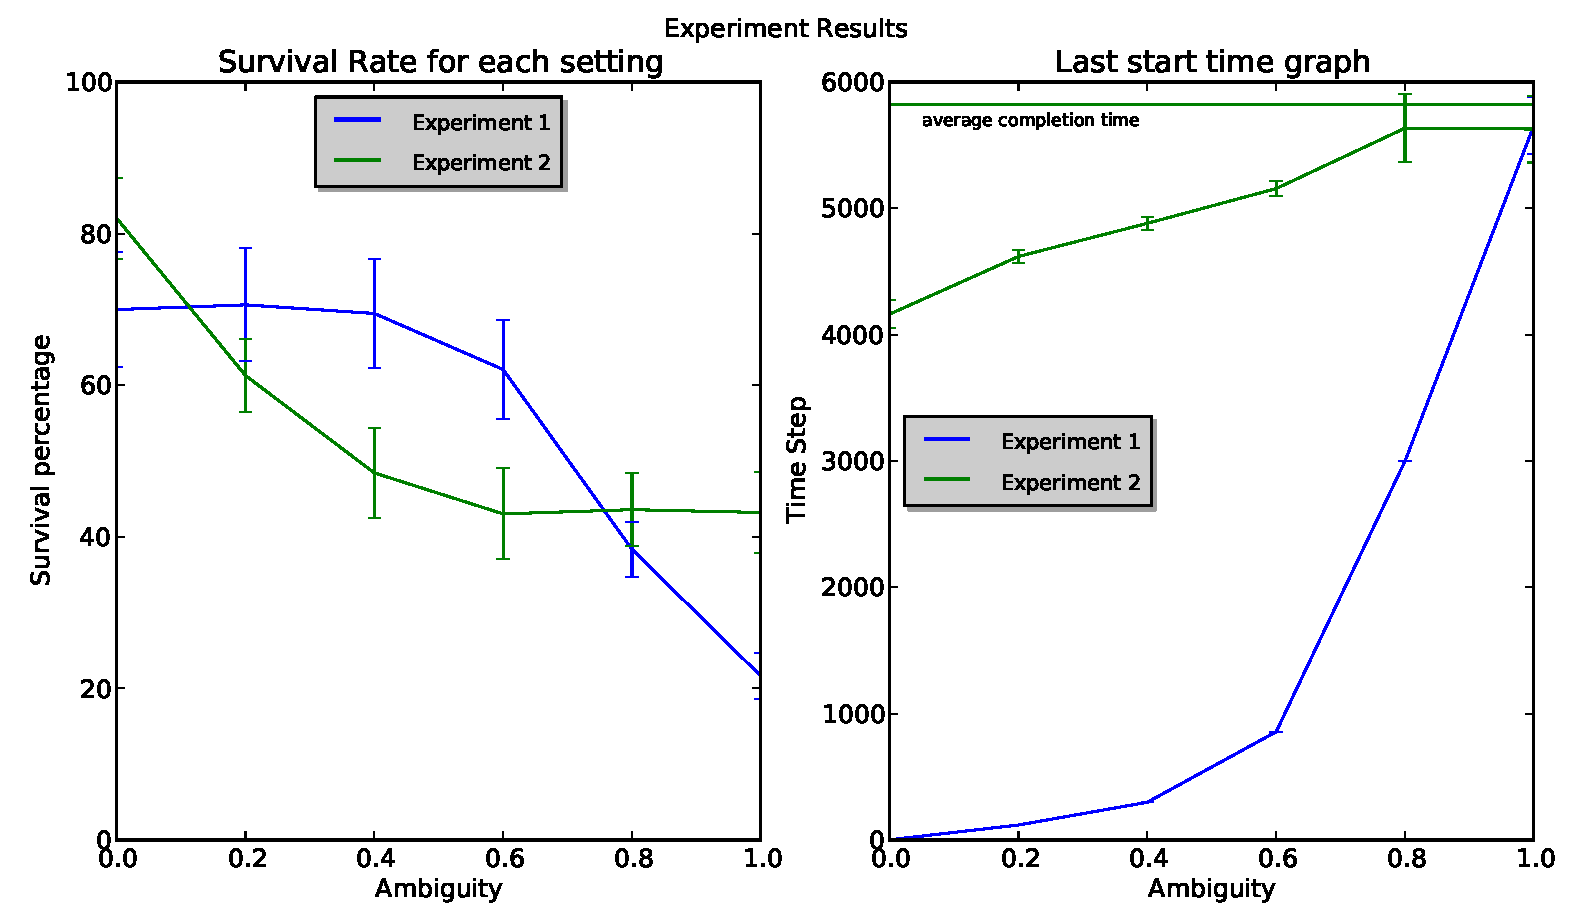
\includegraphics[width=\textwidth]{results}
%   \caption{Observations from 100 replications of each setting of the IBEVAC Simulation}
%   \label{Exp}
%  % Change graph to have average survival rate instead of average number survived.
% \end{figure}
\begin{figure}[!tb]
   \subfloat[Average Survival Rate]{\label{Graph1}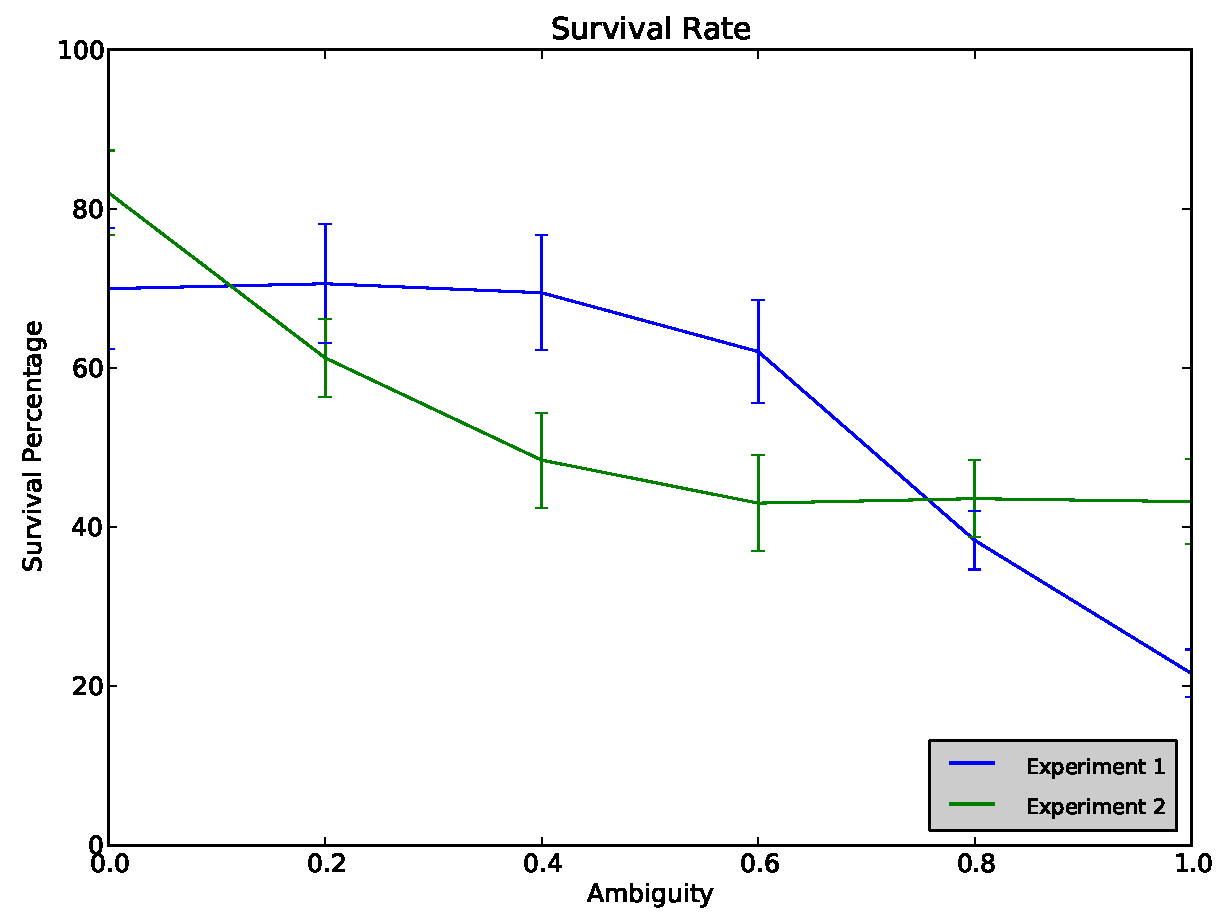
\includegraphics[width=6cm,height=6.2cm]{Exp1}}
   \subfloat[Last Agent Start Time]{\label{Graph2}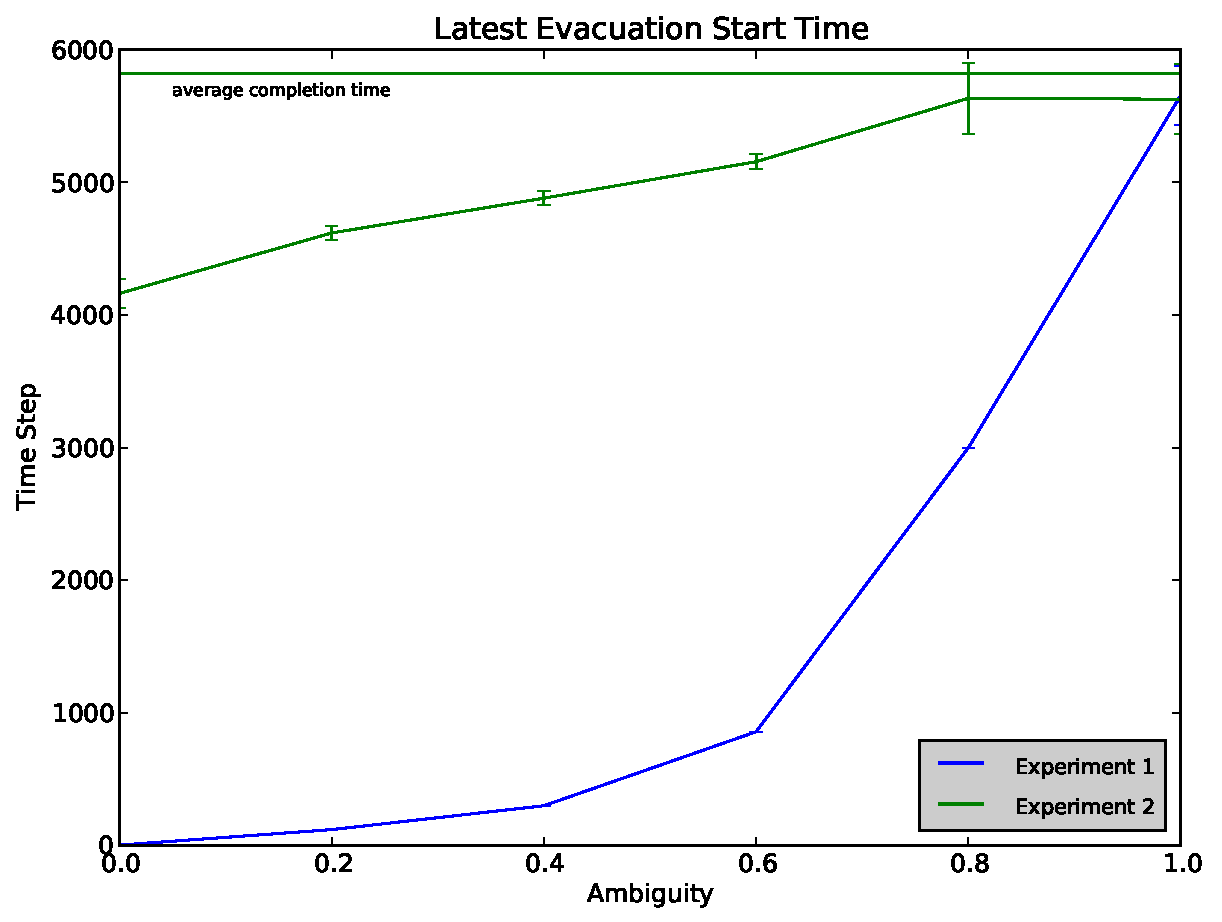
\includegraphics[width=6cm,height=6.2cm]{Exp2}}
  \caption{Observations from 100 replications of each setting of the IBEVAC Simulation}
  \label{Exp4}
 % Change graph to have average survival rate instead of average number survived.
\end{figure}


\section{Conclusion and Future Work}
\label{ConclusionAndFutureWork}

In this paper, the IBEVAC agent architecture for agent based simulation of emergency egress was introduced. A novel cue modeling and perception system which enables the detailed modeling of pre-evacuation behavior has been described and its working demonstrated.

Only preliminary experiments and results were presented in this paper. Further experiments are being conducted in examining the effect of partial knowledge, variability in trustworthiness and other factors. An interesting extension to the cue perception system would be the implementation of a cue memory. This can be used to model agents forgetting about certain cues or being desensitized to cues due to overexposure.
    %!TEX root = vaisagh_thesis.tex

\chapter{A Game-based Investigation into the Role of Memory in Human Exploration and Navigation}
\label{chapter:SpatialKnowledgeChapter}
\chaptermark{Investigating the effect of memory on Indoor Wayfinding}

Several studies have shown that during egress people tend to take routes that are familiar to them rather than the shortest route~\cite{Mawson:2005tq,Paulsen:1984ti,Ramachandran:1990wj,Sandberg:1997tw}. This is because, in most cases, occupants of a building do not have a complete cognitive map of its layout. This is sometimes the case even after the occupants work in the building for several months~\cite{Moeser01011988}. However, existing agent based models of egress, generally make the simplifying assumption that occupants have complete knowledge of the environment. In the rare cases like~\cite{Pelechano:2006ba} where partial knowledge is modeled, it is simply assumed that people have an eidetic memory and never forget a room that they perceive once. Moreover, it is arbitrarily assumed that agents explore unknown environments in either a depth first or a breadth first manner. How people explore unknown environments and gain spatial knowledge from this will obviously have an impact on the paths that are taken during egress. However, a major difficulty in modelling spatial knowledge accurately is our limited understanding of the role of memory in indoor wayfinding and exploration. In this chapter, we try to address this issue.






% THe problem we want to solve
How humans gain and store knowledge of their surroundings has been an area of research for several decades now~\cite{lynch_image_1960,Thorndyke1982560,Kuipers78,Siegel19759,Kuipers01012003}. A significant amount of research has been conducted in trying to understand how wayfinding is done using this knowledge in outdoor environments~\cite{Kuipers78,Gopal1989309}. However, there has been much less work done on indoor exploration~\cite{Kuipers01012003,HolscherBMS06,stankiewicz2006lost,stankiewicz2007acquistion}. With the increasing number of shopping malls, airports, high rise office buildings and residential towers, there is an increasing likelihood that the occupants of a building may not be regular visitors and as a result will have very little knowledge of the layout. If in such a situation, there is a need to evacuate the building, it is important for planners to know how the occupants would react and find their way to the emergency exits. However, there are several aspects of how people explore an unfamiliar environment and the interaction between exploration and memory during this process that is still not understood. More importantly, we believe that existing methods for studying this interaction are limited in certain ways.

% LImitations of most existing work
Understanding how people navigate and explore unknown spaces is scientifically challenging. One of the primary reasons is that experimentally studying such processes  is difficult and time consuming. Even after an experiment is designed, it is often difficult to scale the experiments to many participants and therefore account for various forms of sampling bias. This can be seen in several existing studies like~\cite{Kuipers01012003,stankiewicz2006lost,stankiewicz2007acquistion} which, despite having experiments that are excellently designed, suffer from having few participants and thus probably being susceptible to sampling bias.

% Possible solutions
%mhl - add more references, try to find good ones from psychology
Recently, Bode and Codling~\cite{Bode2013347} demonstrated a possible solution to this problem by using a point and click game to study exit route choice during evacuation and getting more than 150 participants to participate in their experiment. Recent years have seen the emergence of serious games (or gamification) as an approach for conducting human subject experiments~\cite{Anonymous:2011ba,Aydt:2011wz,Michael:2005:SGG:1051239,Waller:2002we}. This approach can elicit the same behavioral response as real world experiments~\cite{Montello:2004uj} while reducing the overhead associated with conducting large-scale real world experiments. In the past this type of approach has been used for validating crowd simulation models~\cite{npelechano:2008ug, Anonymous:2011ba, Viswanathan2014} and understanding behavioral responses to dynamic information during egress~\cite{Bode06022014,Viswanathan:ut}. Serious games~\cite{Michael:2005:SGG:1051239} have a long history in training, for example, aircraft simulation~\cite{hays1992flight} and medical training~\cite{jama.282.9.861}.

%In this chapter games are used only to observe the participant behaviors, whereas for training, the objective is both to observe and steer behavior.

Due to the nature of the data under consideration, namely spatio-temporal tracks of many individuals, \emph{desktop virtual reality experiments} are the most practical way to conduct such experiments~\cite{stankiewicz2006lost,stankiewicz2007acquistion}. For exploration in particular, the use of a virtual environment allows the experimenter to design particular structures and understand how they affect people's decisions. We believe that packaging the experiment in a game, rather than as a standard social experiment, is an ideal way to scale to large sample sizes.

In this chapter we adopt the same methodology to gain an understanding of how humans, with no knowledge of an environment, explore. The method involves experiments in which participants play an exploration game; in the game, they are asked to explore a multi-floor building and complete a set of tasks within a certain time limit. All the movement and actions of the players are logged and later analyzed for patterns. We then propose a novel way of identifying the role that memory and {\em non-randomness} plays in human exploration from the data extracted.
Thus, the main motivations of this chapter, and therefore its main contributions, are :
\begin{enumerate}
\item The development of a novel and scalable game based methodology to study indoor wayfinding behavior.
\item The demonstration of such a scalable method's usefulness in determining how memory influences exploration efficiency and an individual's ability to navigate within an environment.
\end{enumerate}

The remainder of this chapter is organized as follows: Section~\ref{sec:literature_review} first provides an overview of our current understanding of how people gain spatial knowledge and do indoor wayfinding. Following this, the game and experiment are described in Section~\ref{sec:experiment_performed_minecraft}. The methodology used for evaluating the results from the grame are then explained in Section~\ref{sec:methodologies}. Finally, the results and its implications are discussed in Section~\ref{sec:analysis_of_experiment_results}.\footnote{This chapter has been submitted to Nature Scientific Reports for review.}

\section{Literature Review} % (fold)
\label{sec:literature_review}

% Bo An: This section is a bit loose. Rather than just listing some related work, you may also discuss their limitation and say something about how your approach overcomes their limitations.

Human exploration of indoor environments is a complex process that may depend on many factors including the perception of the environment, the person's existing knowledge and various cultural factors. Before examining existing models of human exploration it is useful to establish a basic knowledge of how spatial knowledge is stored, used and updated in human memory. In the context of this chapter, it is also useful to understand the methodology used in studying human spatial memory as both an inspiration and validation for the methodology adopted here.

\subsection{Working memory} % (fold)
\label{sec:spatial_information_in_human_working_memory}


Since Hebb's work on human memory~\cite{DOH1949}, it has generally been accepted that human memory has a Short Term Memory (STM) component and a Long Term Memory (LTM) component. Baddeley's model of working memory~\cite{BaddeleyHitch74}, which is a three component model consisting of the central executive, a visual spatial sketchpad and a phonological loop is currently one of the most popular models of the working of human memory. Central to this idea is the concept of \emph{working memory}. Working memory consists of both a visual and a verbal component both of which are limited in capacity.


In order to study the use of memory during wayfinding, Lindberg and G{\"a}rling~\cite{lindberg1981acquisition} presented people with a difficult task to complete (backward counting), while concurrently performing wayfinding. They discovered that the concurrent task adversely affected wayfinding performance. This supported the notion that navigation may require effective use of limited capacity cognitive sub-systems. However, the relative involvement of different cognitive sub-systems could not be determined through this experiment. Several studies~\cite{Garden1992, meilinger2008working} have involved experiments examining the way in which wayfinding memory is stored. These studies concluded that when maps were used for learning, only the visuo-spatial component of memory was used. However, in the real world, they found that all the senses were used together and that verbal, visuo-spatial, temporal, auditory and even olfactory cues were used by the participants. This supports the notion that experiments studying wayfinding without maps should be as immersive as possible to ensure they reflect reality.

Evidence suggests that salient (distinctive) cues are important for place learning. This is especially true as people age and reduce their ability to perceive and process cues~\cite{Davis01122009} or if the way-finders are stressed or under time pressure~\cite{Ozel:2001tn}. This is quite probably due to the fact that both stress and old age can reduce working memory capacity. A decreased working memory capacity implies a smaller amount of environmental information is processed and less information is eventually encoded. This, in turn, implies that only cues that have high perceptual, cognitive or contextual salience are perceived~\cite{Davis01122009} in stressful situations like emergency evacuations that are the main subject of this thesis.

In summary, human working memory consists of different components for processing different types of cues. Experiments show that different cues are used during wayfinding and thus an experiment to study this behavior should be as \emph{immersive} as possible. Also, wayfinding behavior is likely to be different in stressful scenarios due to cognitive constraints in cue processing. Thus, recreation of a stress or time pressure is necessary to recreate egress wayfinding behavior in experiments.

\subsection{The building blocks of spatial knowledge} % (fold)
\label{sub:how_people_gain_spatial_information}

There are different {\em scales} at which locations are stored in the human mind. According to Sholl and Fraone~\cite{Sholl:2004vu}, these can broadly be divided into 3 levels: Figural Spaces (Object Sized Space), Room Sized Space (Vista Sized Space), Environment Space (Map Sized Space). The accepted approaches and methodologies employed to study and understand these different scales depend on the scale concerned~\cite{Sholl:2004vu}. In this research, we specifically consider Vista and Map sized spaces.

One of the earliest and most influential works on how humans gain and store knowledge of space was Lynch's \emph{The Image of the City}~\cite{lynch_image_1960}. He coined the term \emph{mental map} which refers to a person's perception of the world around him. Perhaps the most important contribution of Lynch's paper was the proposal of the fundamental building blocks of a mental map: paths, edges, districts, nodes and landmarks. Paths are routes along which people move, districts are distinct regions, edges define the boundaries between these regions, nodes and landmarks are locations that are points of reference in the mental maps.

How these blocks form a person's image of space was explored by Siegel and White~\cite{Siegel19759} through their experiments on map learning in children. They proposed a hierarchical model with three distinct parts. They found that people first gain knowledge of the \emph{landmarks} in an area, subsequently they learn \emph{routes} connecting these landmarks and finally they gain \emph{survey knowledge}, wherein they have an overall map of the region to the extent that they can determine shortcuts and best routes. They further postulated that adults, despite having more developed cognitive abilities than a child, mirror a similar process in forming their memory of space.

 Ishikawa and Montello~\cite{Ishikawa200693} emphasized that different people have different abilities and techniques for formation of spatial knowledge. Significantly, they found that given repeated exposure to the environment, some people were inherently good and others inherently bad at forming and using spatial knowledge.

 Some researchers~\cite{Moeser01011988,Ishikawa200693} argue that, contrary to Siegel and White, people's route knowledge and knowledge of space does not significantly improve after first being formed. More interestingly they discovered that certain routes are learned and these routes do not change much; however, inter route connections improve as experience increases.

 In summary, while people do have different techniques of forming and storing spatial knowledge, most studies have confirmed that there is a definite pattern in which it is formed, with landmarks and routes playing a key role at the beginning. Furthermore, studies have also shown that this initial knowledge of routes does not change much with time. This implies that the way in which people first explore an environment most likely plays a key role in determining the route they learn and use. This clearly indicates the crucial role that exploration plays in both short-term and long-term way finding behaviour, thus motivating the need for a better understanding of the way in which humans explore environments.

% subsection the_pioneering_work (end)
\subsection{Wayfinding in indoor environments} % (fold)
\label{sec:indoor_wayfinding}

Literature on human behavior in internal environments, in general, is much more limited than on outdoor wayfinding. \cite{best1970direction} was the first to identify that the number of choice points, that is, locations where directional changes occurred, was the relevant measure for assessing way finding difficulty, as opposed to simple metric distances.


\cite{Weisman01031981} defined visual access, degree of architectural differentiation, signs and floor plan configurations as the factors that determine wayfinding difficulty. \emph{Visual Access} which, in essence, refers to the fact that an environment's external structure gives clues to the internal layout and hence visual access to the outside can decrease wayfinding difficulty.  The findings of~\cite{garling1983orientation} confirmed the importance of familiarity and visual access.~\cite{evans1980cognitive} discovered that distinct wall colors reduced wayfinding complexity.

\cite{Thorndyke1982560} established that map learning can result in survey knowledge developing within 20 minutes. However, if knowledge is gained through actual daily movement through the environment without the use of maps and compasses then it may take up to 2 years for survey knowledge to be developed. This was further tested by~\cite{Moeser01011988} in their experiments with nursing students in a five-floor hospital building. They discovered that floor plans were never used and that even after 25 months, most nurses don't seem to develop survey knowledge. They rather created an image of the layout of the building within the first month and later experience just extended this in minor ways.

 According to~\cite{Gopal1989309}, paths with more choice points like intersections or turns are considered more complicated than paths with fewer choice points. This is a natural consequence of the fact that there is a higher chance of error. More interestingly, they state that paths with more turns are perceived to be longer as well.

 Kuipers'~\cite{Kuipers78,Kuipers01012003} developed the TOUR model of spatial knowledge processing for \emph{large-scale urban spaces} which was one of the first models of spatial cognition. Part of it was a model for exploration which makes use of existing landmarks. In this model, people explore by maintaining their heading with respect to known landmarks like a tower that can be seen from multiple locations. They return to these locations when required. This exploration methodology was further explored and elaborated in~\cite{Kuipers01012003}. Here, the authors proposed that  there are a small set of paths, which they call \emph{the route skeleton}, which people primarily use for wayfinding. People typically explore along this central route skeleton.  This theory was tested through \emph{desktop virtual reality} experiments. However, due to the time required to participate in the experiment and the amount of effort required it was probably both costly and difficult to get too many participants. Thus the experiments were conducted only on four participants which, we believe, limits the analysis that can be done on the data.

The importance of structural landmarks like T-junctions in wayfinding was demonstrated by~\cite{stankiewicz2007acquistion} using desktop virtual environments. A slightly modified version of the same desktop virtual environment was used by the authors~\cite{stankiewicz2006lost} to study exploration in unknown environments through comparison against an \emph{Ideal-Navigator Model}. They explored the inefficiencies in human navigation in unknown environments by comparing against an ideal navigator, i.e. one who has perfect perceptual processing, perfect map memory and the ideal decision strategy. The agent based analysis discussed in Section~\ref{sec:analysis_of_experiment_results} uses a similar approach. While the experiment structure and the analysis of these experiments are interesting, they were only able to get between three and eight participants for each experiment due to the length of the experiments. Thus there is a risk of sampling bias in their conclusions.

H\"{o}lscher et al.~\cite{HolscherBMS06} conducted experiments to investigate the strategies that people use in exploring multi-floor buildings. The first strategy, discussed earlier, shown by Kuipers et al.~\cite{Kuipers01012003} stresses on the primacy of a set of central paths or a \emph{route skeleton} in way finding.  Another strategy, referred to as the \emph{horizontal position strategy}, was used by very few people and generally proved to be inefficient. In this people would try to get to the correct horizontal location first before they try to find the way to the correct floor. The reduced efficiency of this strategy was a consequence of the fact that the experiments were conducted in a building where each floor has a different layout from the next (as is the case in many buildings). The last strategy, which was used by more experienced participants and also proved to be the most efficient, was called the \emph{floor first strategy}. As the name suggests, this strategy involved the person trying to get to the required floor first and then exploring horizontally to find the goal.


\cite{O'Neill1992319} studied the accuracy of simulated environments in studying wayfinding behavior. Their approach was to examine behavior in a simulated environment and compare it to results from actual experiments. Their findings showed that human behavior in simulated environments was a reasonable approximation of the same real life behavior. Montello et al.~\cite{Montello:2004uj} had a much more comprehensive analysis of the effect of different sources: maps, virtual environments and real world experience. In general, they observed that the more immersive the environment is, the more likely it is to produce realistic behavior from the participants. However, it is important that immersiveness not be equated with realism. It is unlikely that immersiveness by itself is a necessary or a sufficient criteria to illicit realistic behavior from human beings. A well designed yet abstract setup like~\cite{O'Neill1992319} is a good counter example. However, a simple point and click setup like the one used in~\cite{Bode2013347} would probably find it difficult to produce realistic behavior from the participants. It is interesting to note that Stankiewicz and Eastman~\cite{StankiewiczEastman} failed to produce this effect of immersiveness producing more realistic behavior. However, this might have been due to the small size of sample data available.


In conclusion, we find that several different kinds of experiments have been conducted over the years ranging from real world, to simulated environments and even virtual reality experiments. Several factors like architectural complexity and visual access have been identified as contributing to wayfinding difficulty. Studies have also revealed that during real world navigation without maps people tend to form an initial cognitive map of the place and this does not improve much over the short term. Thus, the way an unknown environment is first explored is crucial to determining the cognitive map that is developed. There are several theories for strategies that are used during exploration of a large, unknown environment like a multi floor building; of these, a \emph{floor-first} strategy seems to be the most popular and efficient. Some studies have shown that immersiveness does help produce more realistic behavior. However, existing immersive experiments using desktop virtual reality have generally found it difficult to attract more than a few participants. Using serious games for behavior experiments not only overcomes this but has certain other advantages as well that are discussed in more detail next.


% section literature_review (end)


\section{Benefits of a Game Based Approach} % (fold)
\label{sec:benefits_of_the_proposed_approach}

There are four basic advantages that a well designed game based approach can have as an experimental methodology: Immersiveness, Experimental Control, Interestingness and Ubiquity~\cite{Anonymous:2011ba}.

\begin{itemize}
    \item \textbf{Immersiveness:} Immersiveness or accuracy refers to the fact that game mechanics can be designed to closely reflect reality. As explained earlier,  what is important is that the player perceives the artificial environment created as life-like and therefore, makes the same decision in the game as they would in the equivalent real world scenario. For example, a first person environment with realistic but simple movement and turning behavior will likely reproduce more realistic behavior than a point and click game with a bird's eye view.
    \item \textbf{Experimental Control:} The experimental control allowed is a great advantage that a game based approach shares with other traditional desktop virtual reality experiments. Depending on the development environment chosen, the setup of the experiment can be varied at much less cost in terms of time and effort. For example, in most cases, depending on the motivation of the study, it wouldn't take much effort to do A-B testing by varying small elements in the game like the location of a goal provided enough data points are available.
    \item \textbf{Interestingness:}  Games are generally much more enjoyable than standard social experiments. This not only encourages repeat participation but it also helps obtain larger participation through recommendations. There are several standard game design fundamentals which have been developed over the past four decades of computer game development that can help create this interestingness.
    \item \textbf{Ubiquity:} As discussed in Section~\ref{sec:indoor_wayfinding}, a limitation of existing desktop virtual reality experiments is the limited data that is available since they generally get fewer than ten participants~\cite{Kuipers01012003,stankiewicz2006lost}. While the dataset size was sufficient for some of the conclusions that were made, in several experiments significant conclusions could not be derived. This may be because of the paucity of data. Games can be carefully designed in order to make a repetitive mundane task interesting, which in turn will encourage people to play the game and unknowingly perform the task that is required. Many researchers have collected fascinating statistics as to the number of man-hours spent on gaming around the world. As one example, Jane McGonigal~\cite{McgonigalVideo} has suggested that the average American 21 year old will have spent 10000 hours of their lives playing games, which is approximately the same number of hours that same person will have spent within the education system. On May $23^{rd}$, 2010 the Google main page was changed to include a version of the classic PacMan game, some estimations are that 4.82 million man hours of productivity were lost in a single day (approximately US\$120 million).
\end{itemize}
Thus, if designed carefully, a game based experimental methodology can provide several advantages over traditional approaches. In the next section, we present the game that we developed to study how memory influences exploration efficiency and an individual's ability to navigate within an environment.



% The major advantage of using Minecraft is its ubiquity and the scalability of the data generated from it. As discussed in Section~\ref{sec:indoor_wayfinding}, a limitation of existing desktop virtual reality experiments is the limited data that is available since they generally get fewer than ten participants. While the dataset size was sufficient for some of the conclusions that were made, in several experiments~\cite{Stankiewicz1} significant conclusions could not be derived because of the paucity of data. With over 35 million copies of Minecraft sold world wide, it is theoretically easy to get several hundred or even thousands of participants if the game is hosted on a server accessible world wide. This has currently been done and Section~\ref{sec:scaling_the_game} discusses this in more detail. However, in this chapter, we present the initial analysis of the data obtained from the game from 50 participants playing on a local game server.


\section{Setup of the Experiment} % (fold)
\label{sec:experiment_performed_minecraft}


% The previous section discussed a number of different ways in which simulated environments have been used for studying human spatial knowledge. These simulated environments range from Virtual Reality (VR) environments to very simple games of finding a way through a maze.
Wayfinding experiments in virtual reality environments consist generally of two parts: Knowledge Acquisition and Task Performance based on this knowledge. Most existing experiments try to control the knowledge acquisition part of wayfinding. A typical example is~\cite{meilinger2008working} where the author ensured that all participants received identical stimuli in order to be able to fairly compare their task performance based on this knowledge acquisition. Participants were asked to watch a video rather than actively navigate through the environment. This has been the typical approach to date and this has resulted in there being very little existing literature on how people actually explore environments; we believe that the paths taken during exploration could reveal interesting aspects of human exploration.

In order to test this hypothesis and understand more about the way in which humans explore environments and store spatial knowledge, we created a game that requires both exploration and wayfinding and analyzed how the game was played. While creating the environment, we strived to ensure that it had enough complexity and diversity to be engaging and invite exploration~\cite{kaplan1983cognition,Montello:2004uj}.
% To reduce the development effort and to allow for flexibility in environment creation, we built the experiment inside the popular game Minecraft~\cite{Minecraft}.

\subsection{The game}
\label{sec:the_game}


The premise of the game is that the player has been teleported into an abandoned palace where eleven people have been imprisoned in different locations spread across the three floor environment. The objective of the game is for the player to free the eleven prisoners and subsequently follow instructions to open the main gate to the palace and escape. The palace is a three floor building with 44 rooms. The layout of each floor of the palace is shown in Figure~\ref{fig:FloorPlans}. A player joining the server is spawned at the location indicated on the map with an X.

% \begin{figure}[!tb]
% 	\begin{center}
% 		\includegraphics[width=\textwidth]{SpatialKnowledge/introScreenshot}
% 	\end{center}
% 	\caption[Intro screen of Minecraft Game]{This figure illustrates the screen that greets the player on starting the game. The player is lead by similar signboards to the first prison as a tutorial on how to play the game.}
% 	\label{fig:introScreenshot}
% \end{figure}

During the first few minutes of the game the player is presented with the story line and interactively told how to use the controls and play the game through a set of signboards. They also follow a tutorial which helps them free the first prisoner. Subsequently, the player is tasked to find and free the remaining ten prisoners. The locations of the prisons, as shown by the shaded areas in the map, are spread all over the building. This is the first knowledge acquisition phase of the game and we call this the \emph{exploration phase}. This phase requires the player to move around and explore the building. This phase can be reasonably equated to what a new visitor to a building (for example, a shopping mall) experiences.




\begin{figure}[!tb]
  \centering
   % \subfloat[Ground Floor]{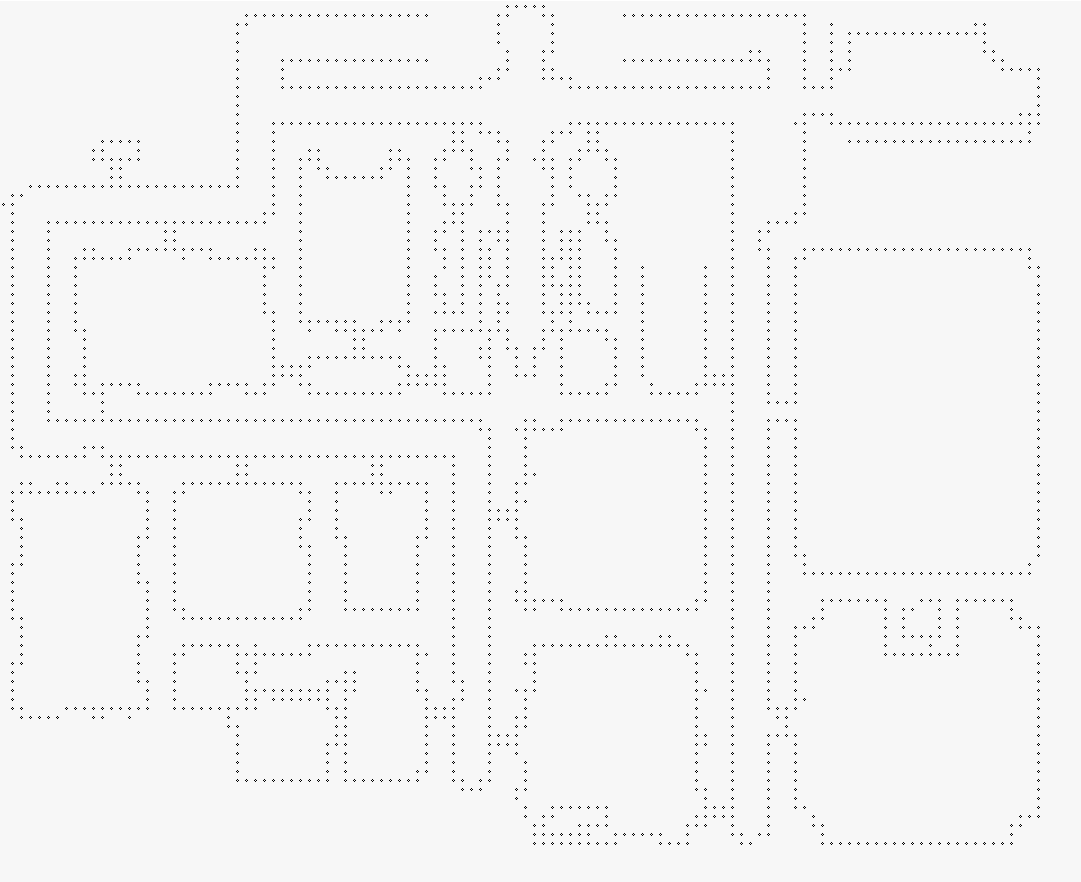
\includegraphics[width=6cm, height=3cm]{SpatialKnowledge/floor0}}
   %  \hspace{1pt}
    \subfloat[Ground Floor]{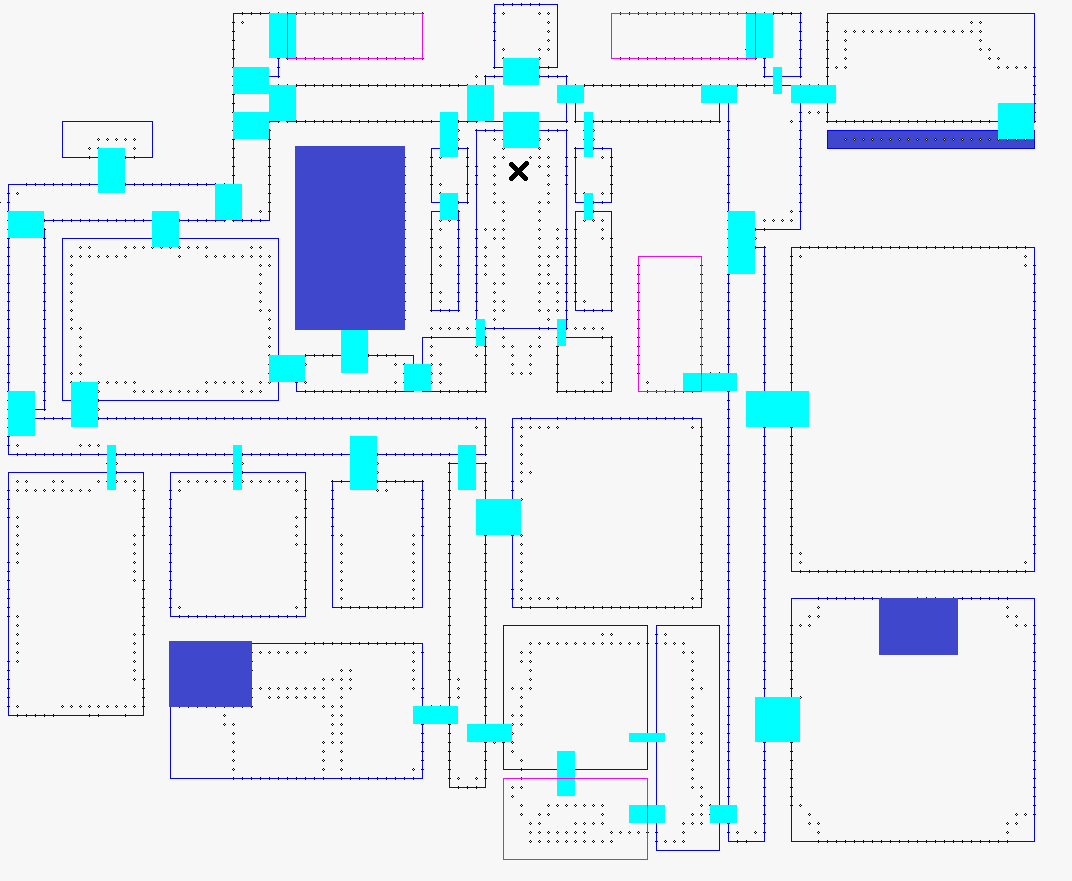
\includegraphics[scale=0.28]{SpatialKnowledge/floor0WithRooms}}
   \\
  %  \subfloat[First Floor]{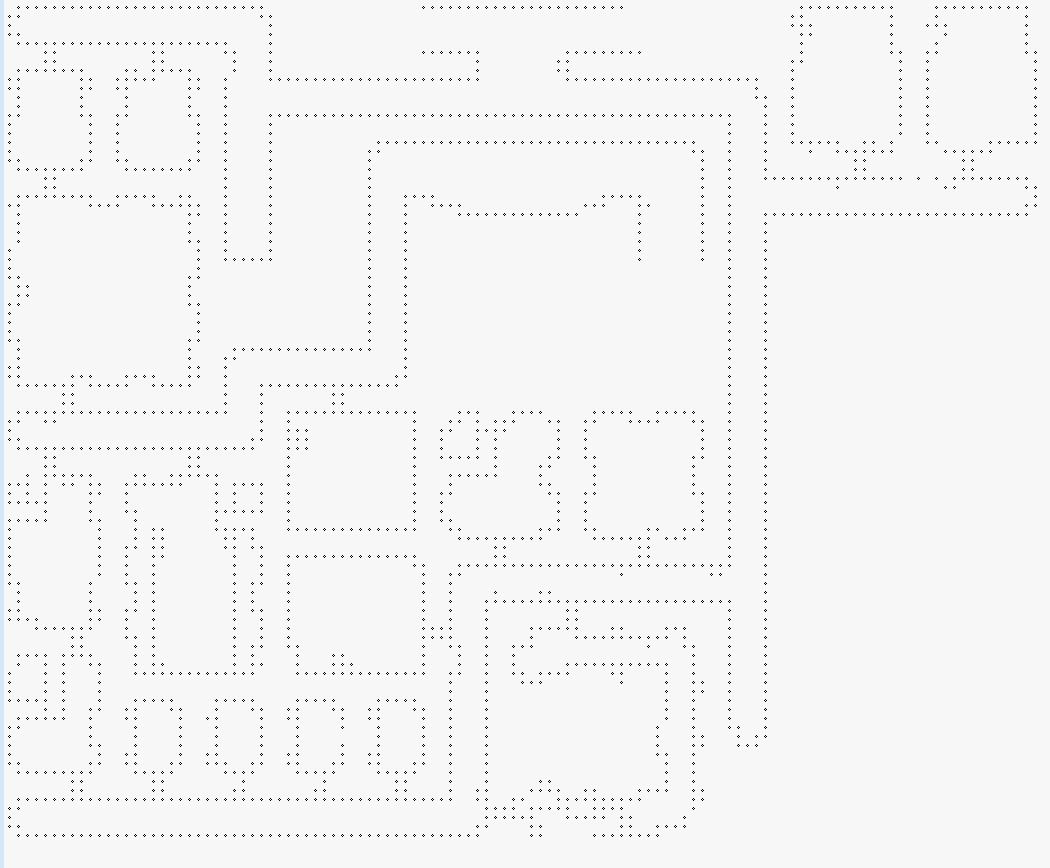
\includegraphics[width=6cm, height=3cm]{SpatialKnowledge/floor1}}
  % \hspace{1pt}
    \subfloat[First Floor]{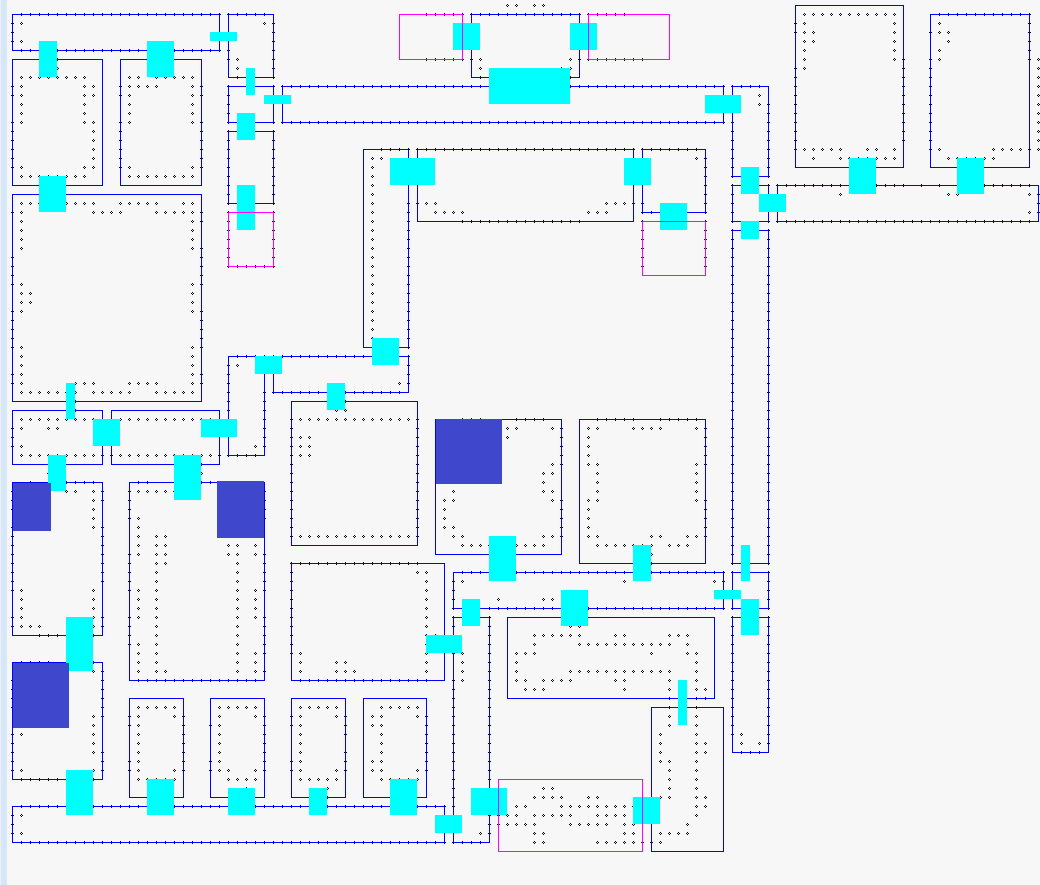
\includegraphics[scale=0.28]{SpatialKnowledge/floor1WithRooms}}
  \\
  % \subfloat[Second Floor]{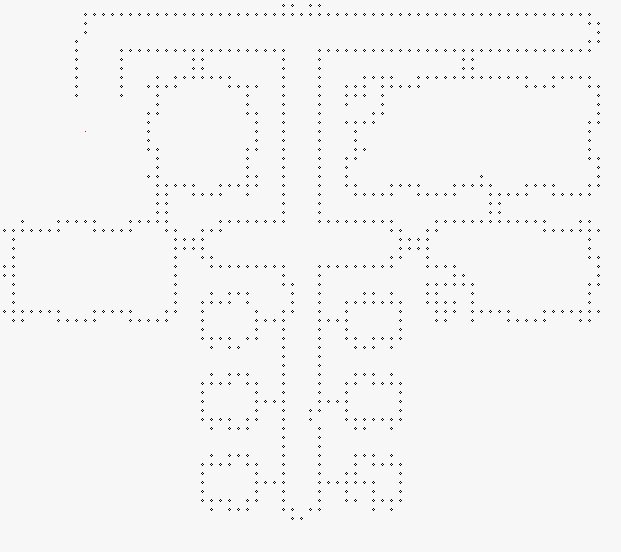
\includegraphics[width=6cm, height=3cm]{SpatialKnowledge/floor2}}
  % \hspace{1pt}
  \subfloat[Second Floor]{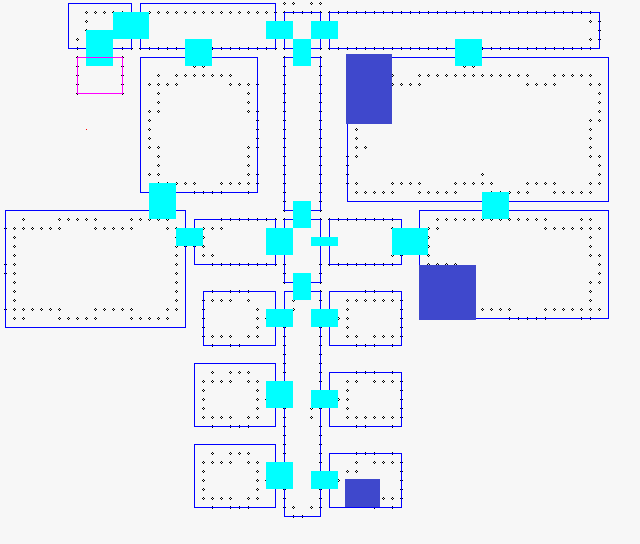
\includegraphics[scale=0.28]{SpatialKnowledge/floor2WithRooms}}
  \caption[Floor Plans of the three floors]{Floor Plans of the three floors. The X indicates the starting point. The blue color indicates the prisoner locations. It is a modified version of an existing Minecraft map~\cite{RoyalPalaceMap}}
  \label{fig:FloorPlans}
\end{figure}



The next phase, which we call \emph{knowledge testing phase}, starts when the eleventh prisoner has been freed. During this phase, the cognitive map formed by the player is tested through a series of three tasks, which involve operating switches that were hidden during the exploration phase. By not revealing the nature of the second phase to the player at the beginning of the game and also by hiding the location of the knowledge testing tasks, we ensure that the player does not make a special effort in remembering locations which could artificially alter the cognitive map formed.

When the eleventh prisoner is freed and the exploration phase ends, the player is given instructions to proceed to the gallery room (shown in Fig.~\ref{fig:MinecraftEscapePaintingRoom}). This room would have been examined by the player during exploration. It is the only room in the palace whose walls are covered with paintings and this makes it reasonably likely that the player will remember this location because of its \emph{perceptual salience}~\cite{Davis01122009}.
% Majority of the players remembering this location indicates that perceptua is indeed a key factor in remembering locations.


\begin{figure}[!tb]
    \begin{center}
        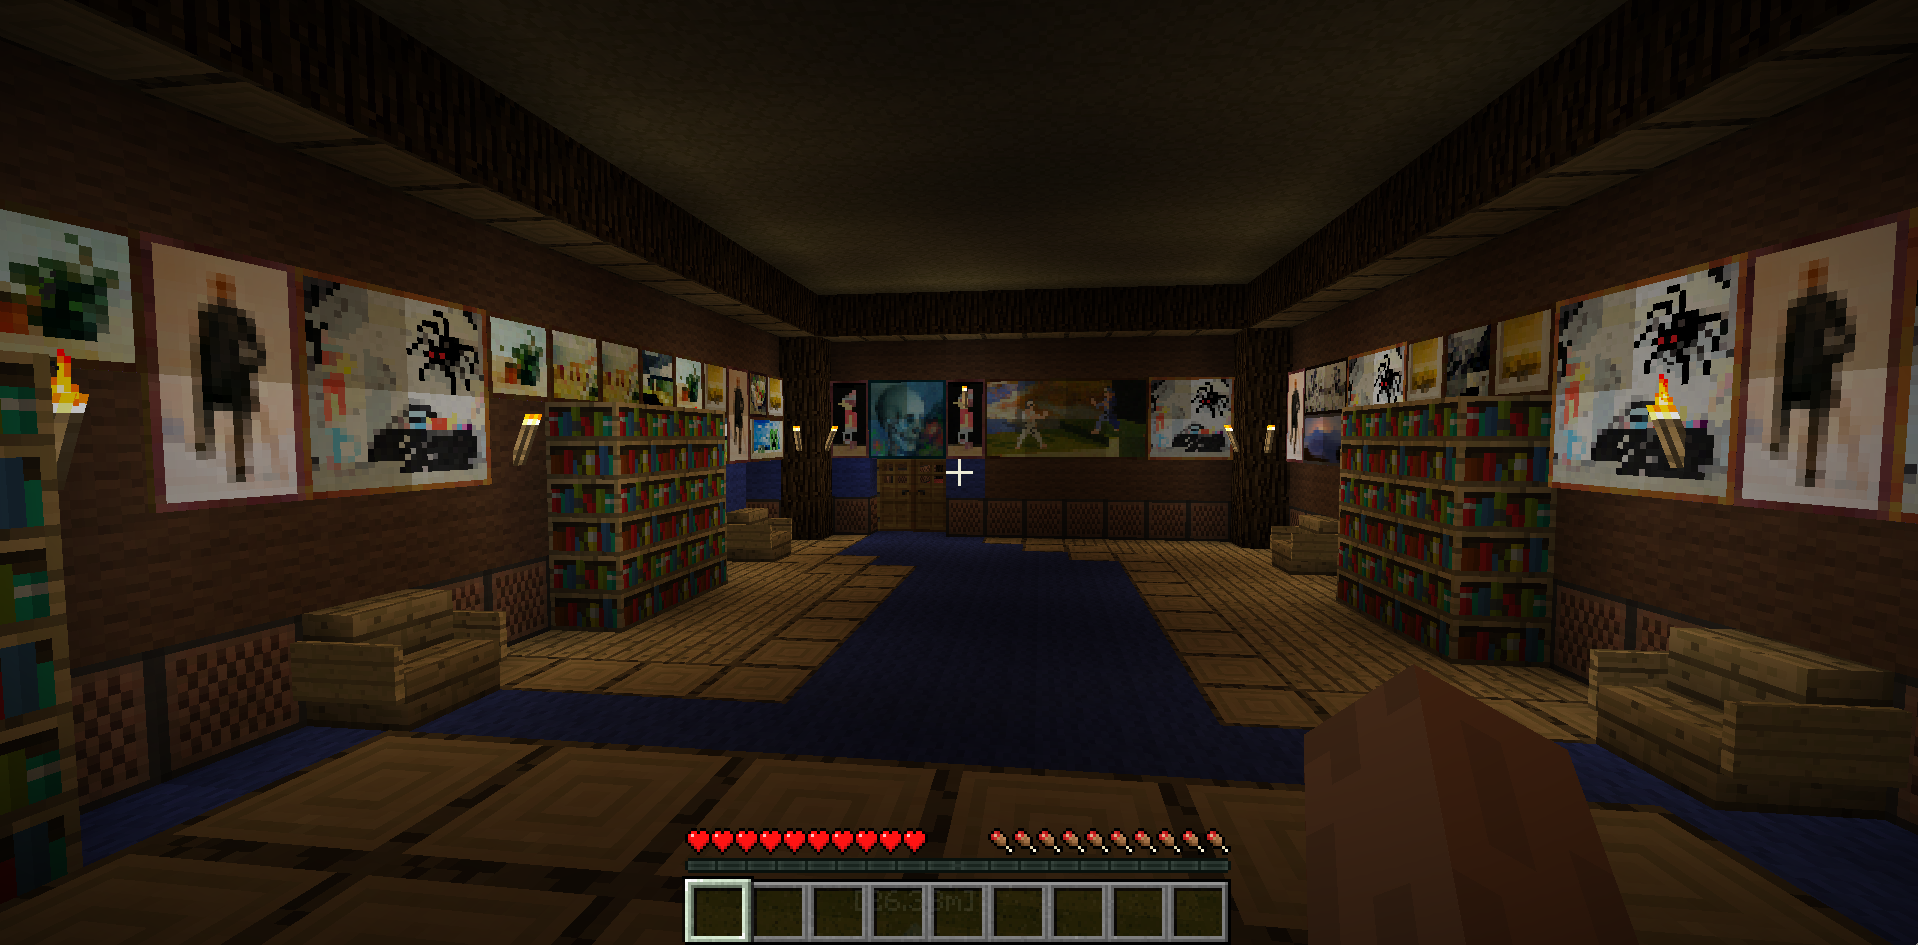
\includegraphics[width=\textwidth]{SpatialKnowledge/PictureGallery}
    \end{center}
    \caption{Picture Gallery}
    \label{fig:MinecraftEscapePaintingRoom}
\end{figure}
%mhl - perhaps give a screen shot of the gallery?

Once the player locates and presses the switch that is revealed in this room, the player is given instructions to move to the second floor library. There are two important factors for choosing this particular location. Firstly, the library has four entrances and is very likely that the player would have entered this room multiple times during the exploration phase. Secondly, being on the second floor, there are multiple paths to this location from the gallery.
% Preference for a particular route among players would help understand more about his/ her cognitive map.

Once this location is found, the player is given the final instruction to proceed to their starting location to find the final switch that will open the main gate to the palace. Again, there are multiple routes to this location some of which are significantly shorter than others. Also, being a starting location and in a somewhat central location, it is likely that it has been frequently visited and should have some \emph{cognitive salience}~\cite{Davis01122009}. We built the experiment inside the popular game Minecraft~\cite{Minecraft} in order to reduce the development effort and to allow for flexibility in environment creation.


\subsection{The Minecraft gaming environment}
\label{sec:the_minecraft_gaming_environment}

Minecraft~\cite{Minecraft} is a Java based multi-platform sandbox construction game. The game involves players creating and destroying various types of blocks in a first-person three-dimensional environment. In the original game, the player controls an avatar that can destroy or create blocks, forming buildings, structures, artwork and even entire cities on multi-player servers or single player worlds across multiple game modes. Players can break any block and build any block, provided he/she has the resources. Figure~\ref{fig:MinecraftEscapePaintingRoom} gives a better idea of the look and feel of the game.


In the development of the game described in the previous section, we use an existing plug-in~\cite{BukkitPermissions} that constrains players so that they can only move around in the environment and interact with doors and switches, that is, elements that are essential for the experiment. A second modification is used~\cite{MyStatisticsPlugin} to keep a log of the movements and actions of the players and store them in a MySql server for analysis. The player locations at different times, the time at which each prison was opened and the time taken to complete each task in the testing phase are all recorded for this purpose.

Using Minecraft provided several advantages; being a popular game with standard controls and a first person view, immersiveness and interestingness are much easier to achieve. Another useful consequence of the popularity of minecraft is the large community of developers and the number of Java based plugins that are available for modifying the default Minecraft environment. This made it easier to develop the game and make the necessary modifications to make the experiment as required. However, the biggest advantage of using Minecraft is the ubiquity it offers with over 35 million copies sold. If hosted on a publicly accessible server, it would be theoretically not be difficult to get several hundred, if not thousand participants. Efforts that have been made to do this are presented in Section~\ref{sec:scaling_the_game}. In the present chapter, we present the initial results of the game being played by participants on a local server.


% section benefits_of_the_proposed_approach (end)
\subsection{Participants} % (fold)
\label{sec:participants}

Fifty young adults (14 women, 36 men, age range: 18-30 years) were recruited with fliers posted on the Nanyang Technological University Campus. Participants were compensated \$ 5 for their participation in the game. It was played by all participants on the same computer in a lab with minimal distractions.

Participants were given five minutes to familiarize themselves with the controls of the first person game, which involved using the keyboard direction keys for movement and the mouse for altering the move and view direction. A mouse click would allow the player to interact with the environment by either opening doors or freeing prisons. The players were given 45 minutes to complete the game. Of the 50 participants, the data from only 44 participants were used, the remaining six experienced motion sickness from the movement in the first person gaming environment and had to quit playing before the game could be completed. Next, we explain the way in which the data was analyzed.

% section participants (end)
\section{Analysis} % (fold)  % To find a better name
\label{sec:methodologies}

In this section we present the methods that were used to analyze the data obtained from the game. Figure~\ref{fig:UnscaledMap} shows the room layout show in Figure~\ref{fig:FloorPlans} as an undirected a graph. A directed \emph{movement graph} is calculated for each player, with the edges of the graph indicating the direction and time of movement from one node to the next. The analysis presented in the following sections is performed using these graphs.


\begin{sidewaysfigure*}[!htbp]
\centering
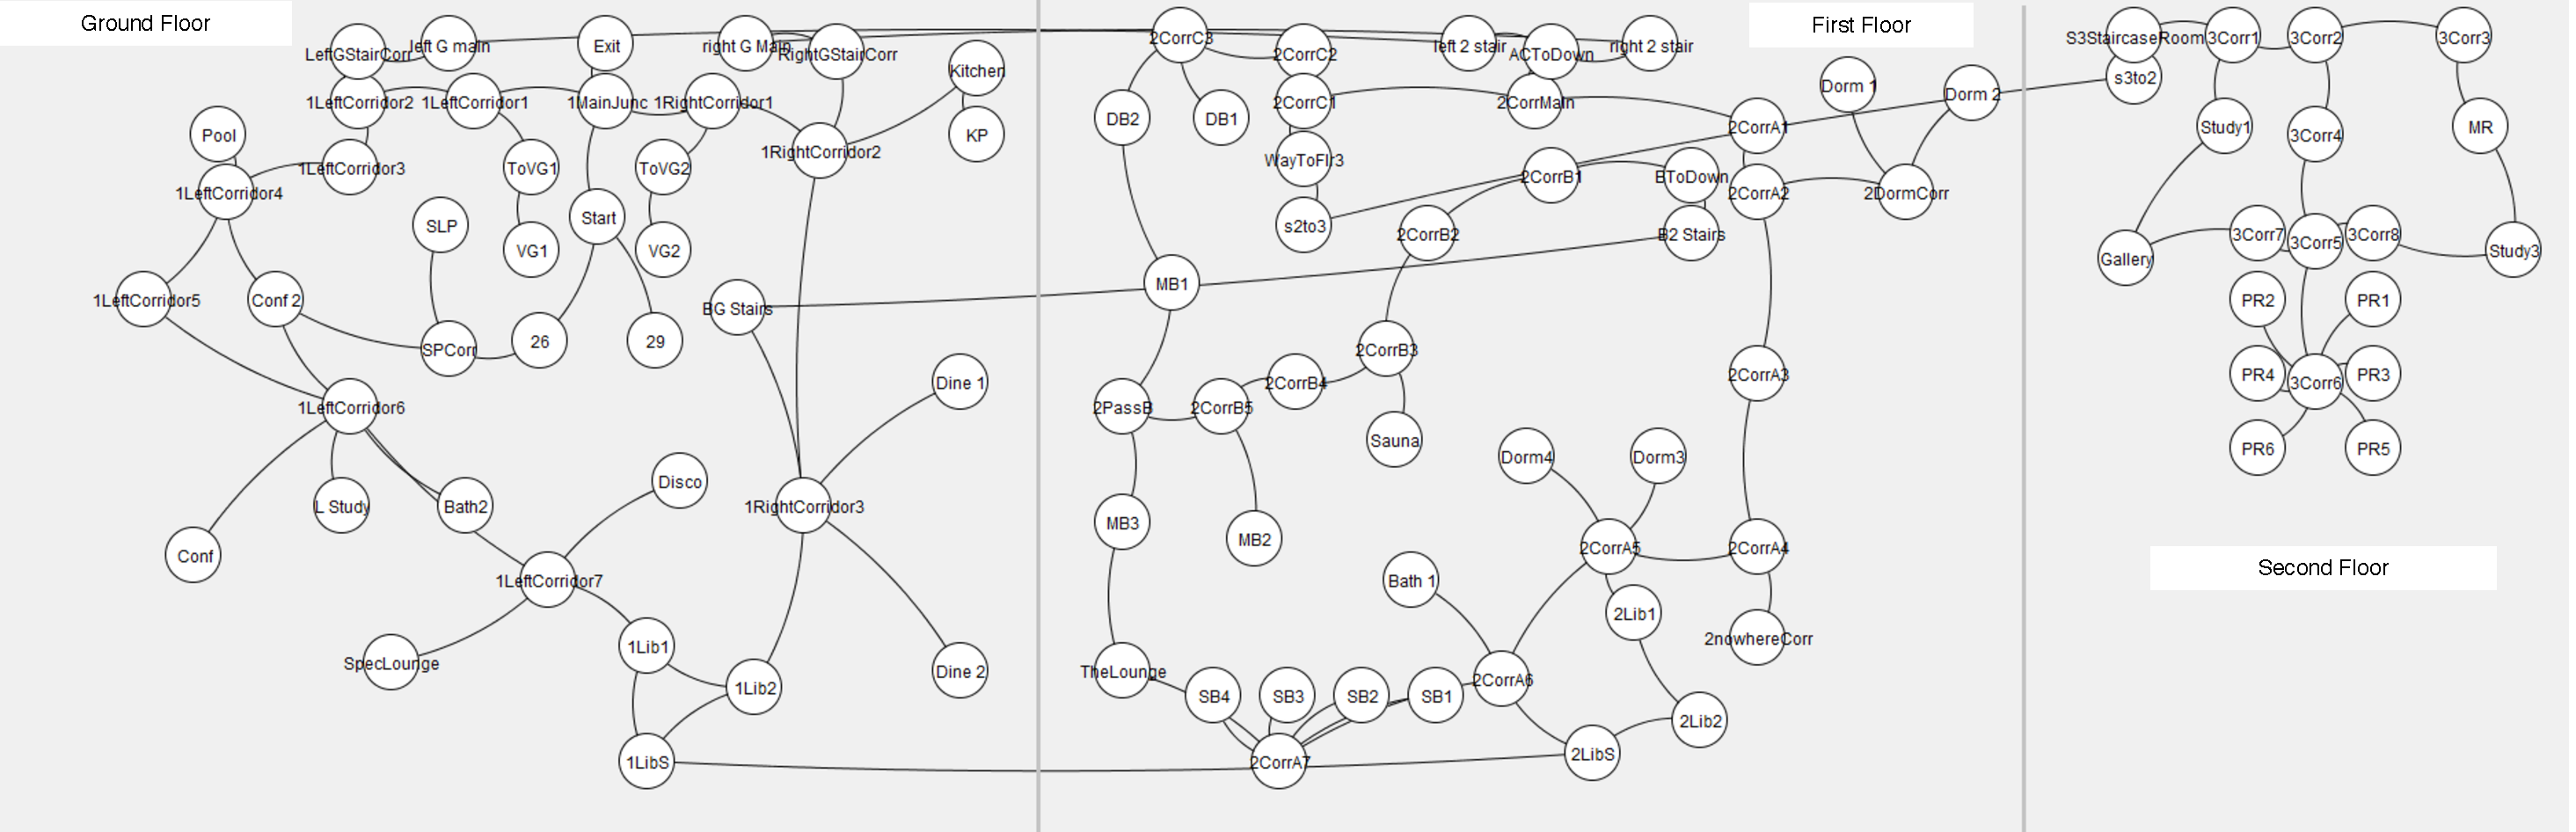
\includegraphics[width=\textwidth]{SpatialKnowledge/unscaledRoomLayout.pdf}
\caption[Graphical representation of floor plan]{This figure shows a graphical representation of the room layout in Figure~\ref{fig:FloorPlans}}
\label{fig:UnscaledMap}
\end{sidewaysfigure*}



\subsection{Types of exploring agents}
\label{sec:types_of_data}

As mentioned in the introduction, the motivation of our analysis is to determine how memory influences exploration efficiency and an individual's ability to navigate within an environment. In order to do this, we use an approach similar to the ideal navigator model of  Stankiewicz et al~\cite{stankiewicz2006lost}. We compare the movement of the players to different kinds of simple exploring agents inhabiting the same environment as the player. By comparing the performance of these simple agents to the actual performance of the player, we determine the ways in which a player is different from or similar to each of these agents.

We compare the \emph{movement graph} of the players to three kinds of exploring agents: Markov agents, unbiased random walkers and agents with perfect $m$-step memory. Just like the actual players, these agents have no prior knowledge and explore the undirected graph shown in Figure~\ref{fig:UnscaledMap}. Our analysis is done based on four sets of directed movement graphs :
\begin{itemize}
    \item \emph{Actual Players}: This is the set of 44 player movement graphs i.e. the movement graphs introduced at the beginning of this Section.

    \item \emph{Unbiased Random Walker}:  The next node to which this agent moves is chosen randomly with equal probability. Each iteration of the random walk is performed until the walker covers $100\%$ of the environment. A collection of random walks is obtained until the variance in the radius of gyration of generated movement graphs stabilizes. The radius of gyration is the standard deviation of a walker's position to the center of mass of movement~\cite{cheng:footprints}. It gives a measure of the locality of the graph.

    \item \emph{Agent with perfect $m$-step Memory}: This is a biased random walker with an $m$-step memory. It moves exactly like the random walker except that it avoids moving back to any of the $m$ rooms it visited previously. If there is no unvisited room, the agent checks its $m$-step memory for an unexplored junction. If such a junction exists, it goes back to that point and continues exploring in an unvisited direction. If such a junction does not exist the agent simply choses,  at random,  a neighbouring location to the current node with equal probability. Depending on the calculation being performed, the path is generated for a specific number of hops or until a specific coverage is achieved. The coverage is simply calculated as:
    \begin{equation}
        \mbox{coverage} = \frac{\mbox{number of rooms visited}}{\mbox{total number of rooms}} \times 100
        \label{eq:CoverageEquation}
    \end{equation}
     $30,000$ such movement graphs are generated for each value of $m$ for each experiment. This was empirically found out to be a good enough value to ensure minimal variation in the radius of gyration.

    \item \emph{$m^{th}$ order Markov Agents}: These agents mimic the movement of the average of the ensemble of players assuming they had only an $m$ step memory. The action of an $m^{th}$ order Markov agent at a particular point in the path is a function of the actions of the actual players who had taken the same $m$ steps. This is explained in more detail in Section~\ref{sec:Markov_data_analysis}. The calculations are performed for m from 1 to 13. As with the agent with perfect memory, the movement graphs are generated either for a specific number of hops or until a specific amount of coverage is achieved. Also, as before, $30,000$ movement graphs are generated for each value of $m$.
\end{itemize}

Simulations of movement were used to generate movement graphs for each of these types of agents and the results of this analysis are presented in Section~\ref{sec:analysis_of_experiment_results}. Before this, the next section explains the working of the Markov agents in more detail.

\subsection{Markov Agents}
\label{sec:Markov_data_analysis}


In this section we present how the movement of the Markov agents are calculated. The chief motivation of this Markovian analysis was to investigate the role that memory plays in the exploration of the environment.

We take an $m^{th}$ order Markov model to represent an $m$-step memory of the explorer, where steps constitute node visits on the undirected graph (Figure~\ref{fig:UnscaledMap}). One way to speculate on the size of the memory used by a human during exploration is to predict a path of length $n$ from some Markov data of order $m < n$.  We hypothesize that \emph{if the movement of the actual players can be predicted using an $m^{th}$ order Markov agent, this implies that humans use a working memory of size $m$ steps during exploration.}

In a general $m^{th}$ order Markov process, the basic idea is that the action at any point of time depends only on the previous $m$ actions. By stating that the process of exploration is an $m^{th}$ order Markov process, we assume that the next node that is visited by a player is only dependent on the previous $m$ steps. This is different from an agent with $m$-step memory that tries to avoid the previous $m$ nodes. Since the next step is dependent on the actions of players who have visited that same subsequence of $m$ nodes, the Markov model theoretically encapsulates other factors like layout, visibility and so forth and thus unlike the former, has \emph{imperfect recollection}.


\begin{figure}[!t]
\centering
        \subfloat[The Situation]{\label{fig:situation}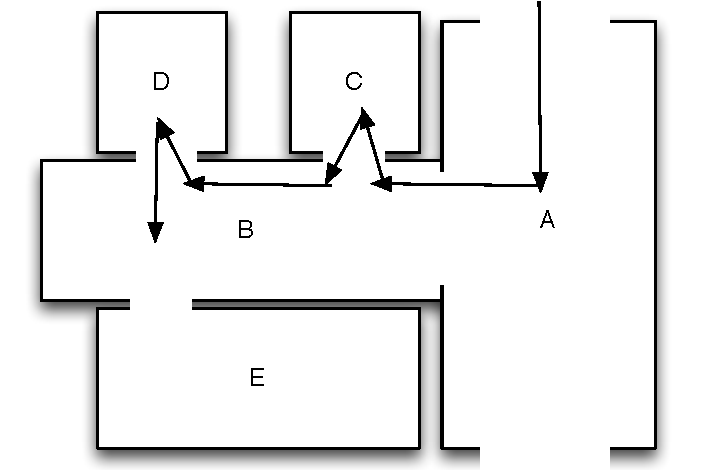
\includegraphics[width= 0.48\textwidth]{SpatialKnowledge/situation}}
    \hspace{1pt}
        \subfloat[Player 1]{\label{fig:player1}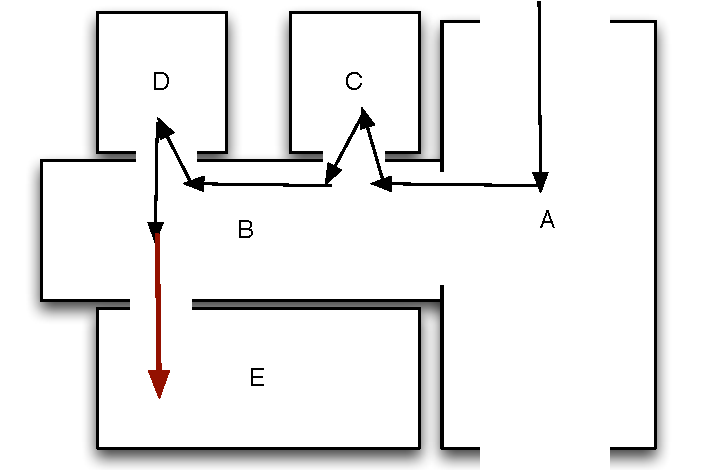
\includegraphics[width= 0.48\textwidth]{SpatialKnowledge/player1}}
    \\
        \subfloat[Player 2]{\label{fig:player2}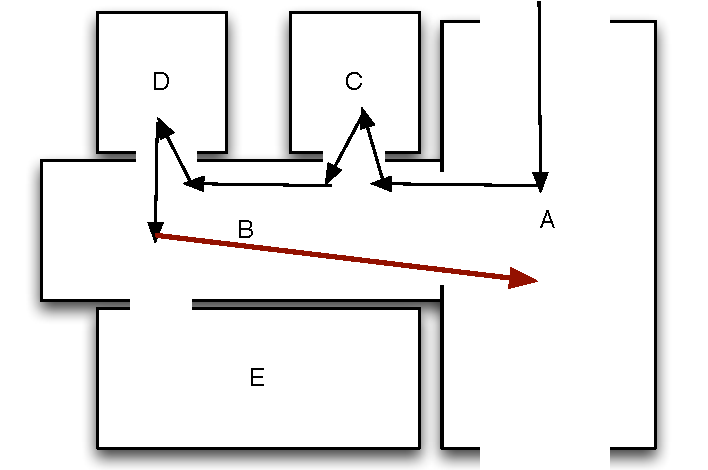
\includegraphics[width= 0.48\textwidth]{SpatialKnowledge/player2}}
    \hspace{1pt}
        \subfloat[Player 3]{\label{fig:player3}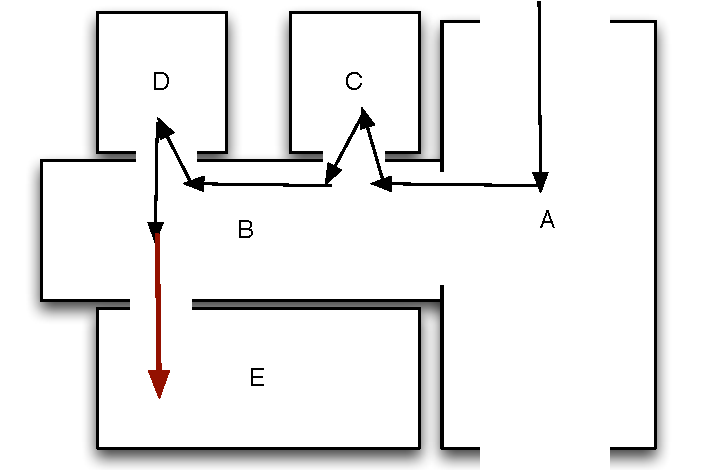
\includegraphics[width= 0.48\textwidth]{SpatialKnowledge/player3}}
    \\
        \subfloat[Agent with 6-step memory]{\label{fig:agent}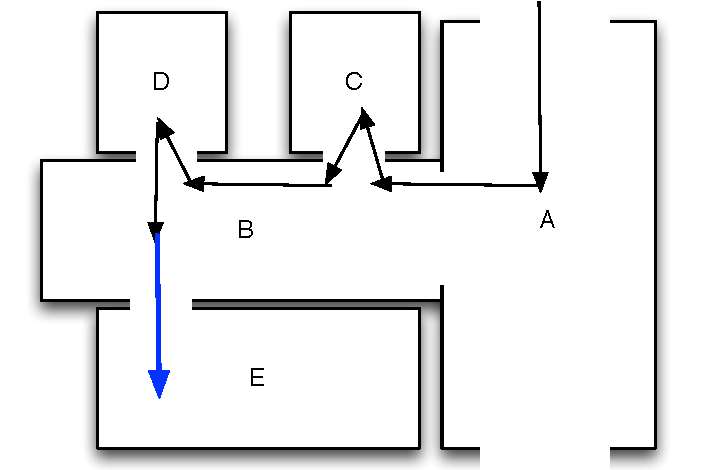
\includegraphics[width= 0.48\textwidth]{SpatialKnowledge/agentWithMemory}}
    \hspace{1pt}
        \subfloat[$6^{th}$ order Markov Agent]{\label{fig:markov}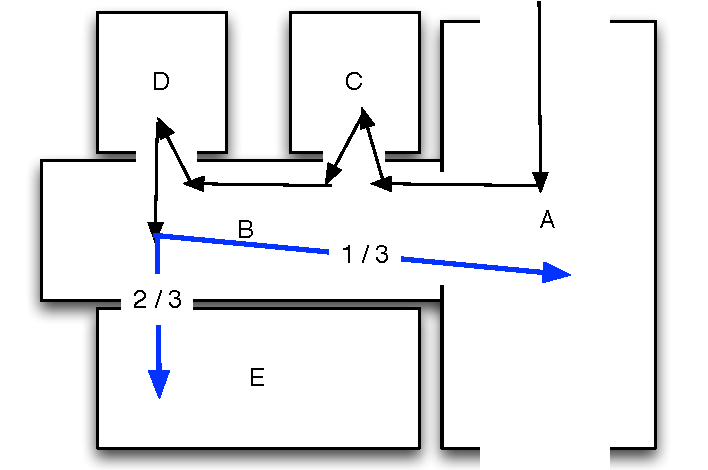
\includegraphics[width= 0.48\textwidth]{SpatialKnowledge/markovAgent}}
    \caption[Markov Data Explanation]{Given the situation in (a), the agent with 6-step memory would move next to room E since it has the list {B,D,B,C,B,A} as the 6 rooms visited immediately previously. However, the action of the $6^{th}$ order Markov agent in this situation is dependent on the actions of the players ((b),(c) \& (d)) who happened to be in the same situation. Since one out of the three players who were in the given situation next moved to room A, there is a $1/3$ chance that the Markov agent will visit room A next.}
    \label{fig:markovExample}
\end{figure}


Figure~\ref{fig:markovExample} explains the idea of a Markov agent by contrasting it's behavior with that of an agent with simple m-step memory. In the example layout shown in figure--- with the rooms C, D and E connected to corridors A and B--- we consider the situation where the exploring agent has moved from A to B to C to B to D and back to B. Assuming a 6-step memory, the simple memory agent would definitely visit room E since all other rooms have been visited in the last 6 steps. However, the Markov agent's action in this situation depends on the actions of the actual players in this situation. Since two out of the three players visited room E and one out of the three players visited room A, the next step of the Markov agent can either be room E or A with $2/3$ and $1/3$ probability respectively. The following section explains in more detail how the Markov agent movement graphs are calculated.
% Interestingly we found significant performance improvements when we reach $m$ of 6 to 8.

% To understand if an $m^{th}$ order Markov model is sufficient for describing exploration efficiency we measure the exploration performance in terms of minimum hops needed and maximum coverage obtained. This is done for different values of $m$ and then compared with the exploration of the unbiased random walker and the agent with perfect $m$-step memory.

\subsubsection{Calculation of Markov data} % (fold)
\label{sec:calculation_of_Markov_data}

\begin{table*}[!bp]
\caption{Summary of symbols and their meaning.}
\label{tab:Symbol_Table}
\begin{tabular}{lcc}\hline

Symbol & Meaning   \\ \hline
$Pr (A|B)$ & Probability of occurrence of event A given event B \\
$X_n$ & Random variable indicating the location in the $n^{th}$ step \\
$p^{(n)}_{ij}$ & Probability of going from state $i$ to state $j$ in $n$ steps \\
$R$ & Set of all nodes \\
$r$ & A particular node \\
$N_r$ & Set of neighbors of node $r$ \\
$P^{(n,D)}$ & List of all paths of length $n$ taken by individuals in dataset $D$\\
$Q^{(n)}$ & Random variable representing a path of length $n$\\
$q^{(n)}$ & A particular path of length $n$\\
$\phi(a,L)$ & The number of occurrences of element $a$ in list $L$\\
$x^{(q)}_{i}$ & The $i^{th}$ location in a particular path $q$\\

\hline
\end{tabular}
\end{table*}

This section explains how the aforementioned Markov calculations are done. These calculations are performed on the \emph{actual player} dataset $D$ derived from the game (Section~\ref{sec:types_of_data}). To recap, a directed movement graph is stored for each player. Each node of the directed movement graph corresponds to a node in Figure~\ref{fig:UnscaledMap} and each edge indicates the movement of the player from one node to the next. Each edge also stores the time point of traversal. The symbols used in this section and their meaning are summarized in Table~\ref{tab:Symbol_Table}.


The $m^{th}$ order Markov probability of visiting a node $b$ from a node $a$ is defined as the probability that the $m^{th}$ node after visiting node $a$ is node $b$. Mathematically, it can be stated as:
\begin{equation}
    p^{m}_{ab} = Pr(X_{m}=b|X_{0}=a)
\end{equation}

It is assumed that it is a time homogeneous process, that is,
\begin{equation}
    p^{m}_{ab} = Pr(X_{k+m}=b|X_{k}=a) \ where\  k \geq 0
\end{equation}



To calculate the $m^{th}$ order Markov data using dataset $D$, we calculate the following:
\begin{enumerate}
    \item First, for each path of length $m$, \emph{the number of times that path is observed} in dataset $D$ is counted.

    From this, the following equation can be used to derive $p^{m}_{ab}$:
    \begin{equation}
        p^{m}_{ab} = \frac{\left\vert{P^{(m,D)}_{ab}}\right\vert}{\sum\limits_{x\in R}\left\vert{P^{(m,D)}_{ax}}\right\vert}
        \label{eq:HeatMapEquation}
    \end{equation}

    \item For each path of length $m$, \emph{the likelihood that a particular path} is the result of $m$ steps being taken is simply the ratio of the number of occurrences of the particular path of length $m$ to the total number of paths of length $m$ in the database $D$; mathematically:
    \begin{equation}
        Pr(Q^{(m)}=q^{(m)}) = \frac{\phi(q^{(m)},P^{(m,D)})}{\left\vert{P^{(m,D)}}\right\vert}
        \label{eq:TableEquation}
    \end{equation}


    \item Using these, we can calculate the probability of each destination given a particular path of length $m$ by using Bayes Theorem.


\end{enumerate}

For $m^{th}$-order Markov agent, given a particular path of length $m$, it is possible to generate the $(m+1)^{th}$ step using the previous $m$ steps, that is, the $1^{st}$ to $m^{th}$ step. This is done using the destination probabilities calculated in step 3. Following this, the $(m+2)^{th}$ step can be predicted by doing the same calculation using the preceding $m$ steps from $2$ to $m+1$. This process can be continued to generate a directed movement graph of $n$ edges using just the $m^{th}$ order Markov data. As mentioned previously, calculations are done using $30,000$ paths generated like this. A question that might arise for the discerning reader at this point is whether the dataset is sufficiently large to do such Markov calculations reliably for large values of $m$. We present further analysis on the validity of this calculation in Appendix~\ref{sec:validity_check_for_markov_analysis}. Next, we look at the results of our analysis.

% section methodologies (end)

\section{Results} % (fold)
\label{sec:analysis_of_experiment_results}

% VVT: WRITE AN ACTUAL INTRODUCTION TO THIS SECTION!!
% In the previous section we introduced the basic techniques that we used for analyzing the data obtained from the games. In this section we present our findings from using these techniques on the data.

% \begin{sidewaysfigure*}[!htbp]
% \centering
% 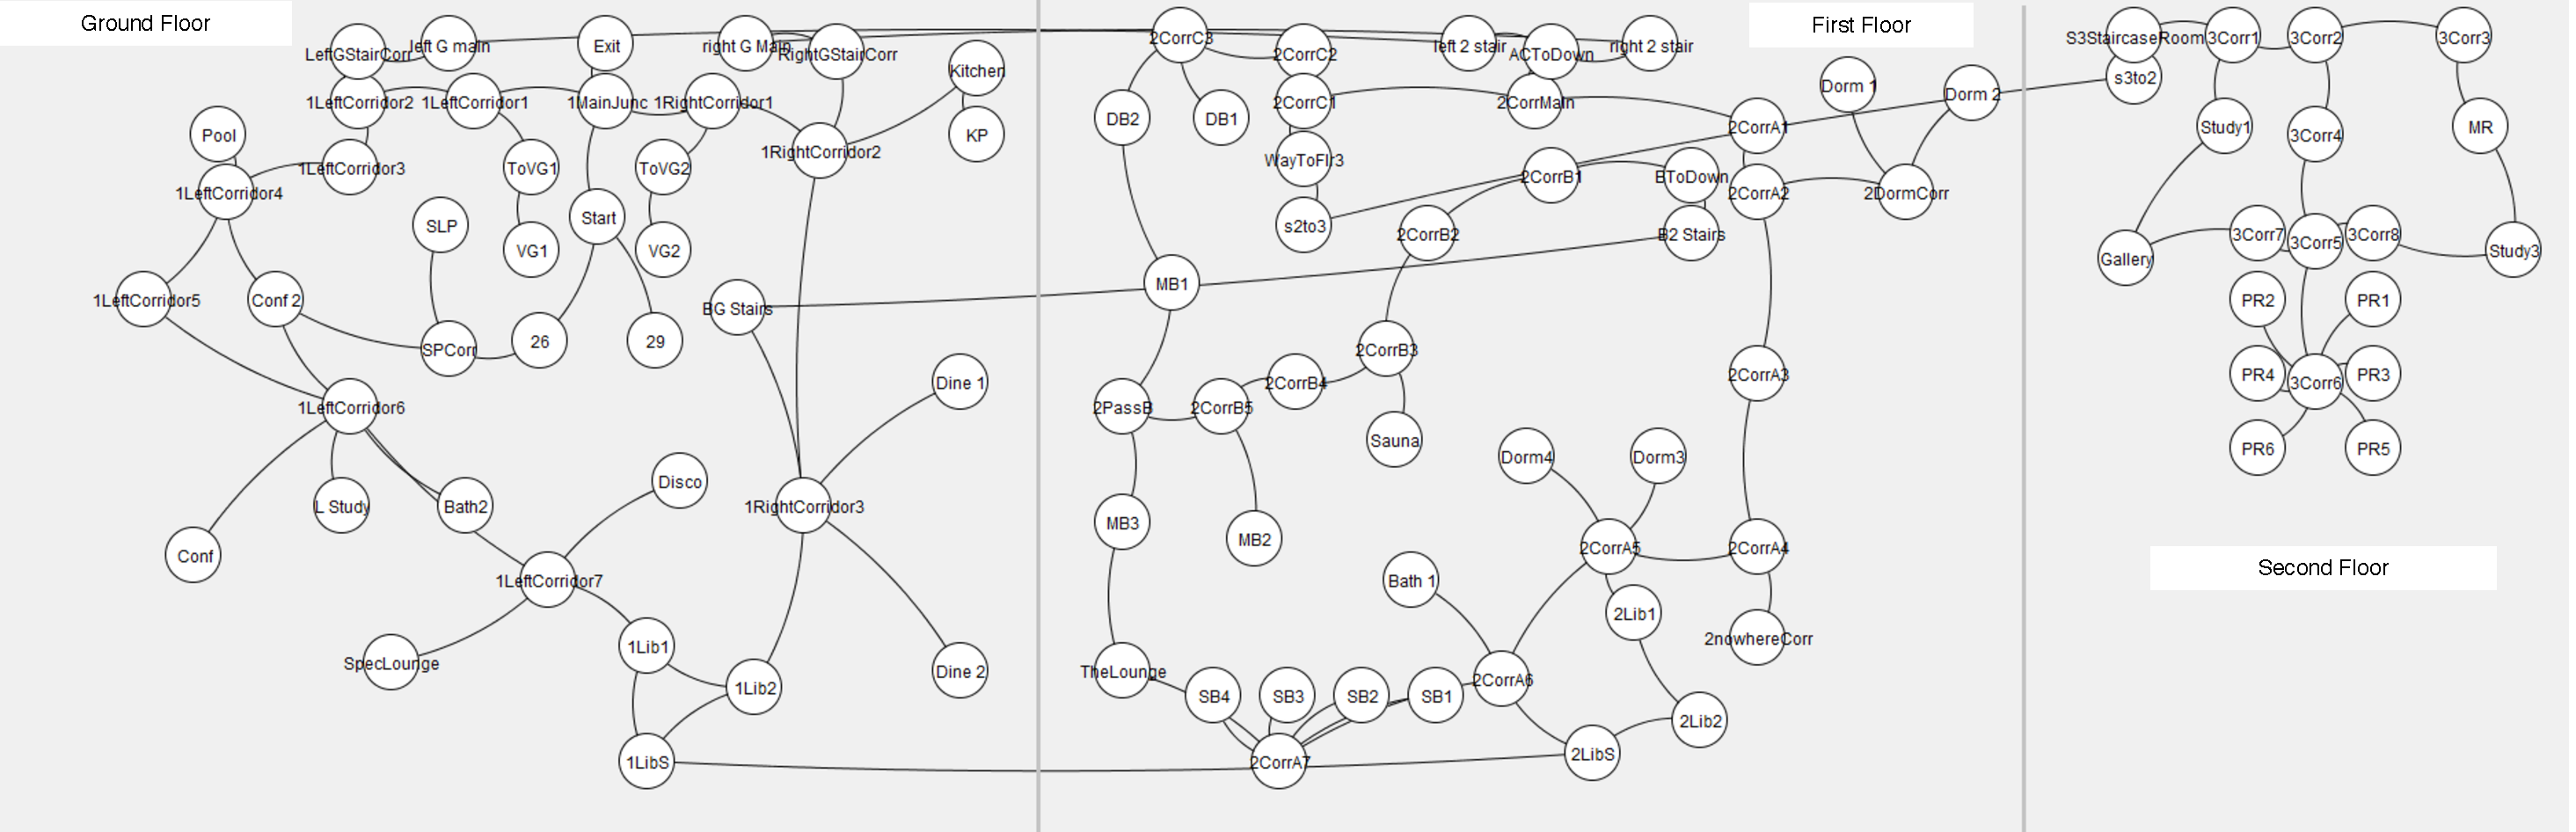
\includegraphics[width=\textwidth]{SpatialKnowledge/unscaledRoomLayout.pdf}
% \caption{This figure shows a graphical representation of the room layout in Figure~\ref{fig:FloorPlans}}
% \label{fig:UnscaledMap}
% \end{sidewaysfigure*}

From the game, the complete movement traces of 50 players were obtained. This data was analysed by comparing against agents of different types to determine patterns and gain a better understanding of the movements of the players. This section presents the results of four kinds of analysis that was performed. First, we present the results of a simple check of the frequency of visits to each room. Following this, we compare the efficiency of movement of the players against the different agents. Finally, we present some empirical observations from the movement graphs of the actual players.


\subsection{Room visit frequencies}


In our first experiment, we calculate the frequency of visits for each room per player and compare this against the unbiased random walker. This is a simple test to determine if the players have a pattern or strategy in their exploration that is different from a random walk. If there is a significant difference in the number of times a particular floor or area of the building is visited by a player then this will probably be revealed by this comparison against an unbiased random walker.

For each room $r$ we calculate the normalized number of visits $\alpha$. For any room $r$, let $f_p(r)$ be the total number of times room $r$ is visited by the the player $p$ and let $f_{rw}(r)$ be the number of times the average random walker visited the same room. We define the normalized number of visits $\alpha$ as:
\begin{equation}
	\alpha_x(r) = \frac{f_x(r)}{\sum_{a \in R} f_x(a)}
	\label{eq:alpha_equation}
\end{equation}
This is calculated for both the player and the random walker. Using this the visit ratio, $y_{p}(r)$, of the actual player is calculated for each room as:
\begin{equation}
y_{p}(r) = \frac{\alpha_p(r)}{\alpha_{rw}(r)}
\label{eq:y_equation}
\end{equation}
A random walker's frequency of visits to a particular node is purely a function of the topography of an environment i.e. the nodes and their connectivity. Thus, unlike $\alpha_p(r)$, $y_p(r)$ would not contain the effects of the degree of a node. This means that if a room $r_1$ has lower value of lower $y_p(r)$ than $r_2$, this is not because of the room having lesser connectivity. The average $y(r)$ over the ensemble of player data was then calculated. This is illustrated in Figure~\ref{fig:scaledMap}. This figure shows the value of $y(r)$ of each room as a scaled version of Figure~\ref{fig:UnscaledMap}. The red color indicates those rooms that have $5\%$ more visits than a random walker and the green color indicates those that have $5\%$ less visits than a random walker; the node is colored white otherwise. The diameter of each node in this graph is scaled to $y_r \times \mbox {unscaled diameter}$.

\begin{sidewaysfigure*}[!htbp]
\centering
\includegraphics[width=\textwidth]{SpatialKnowledge/scaledGraph.pdf}
\caption[Visualization of room visit frequencies]{Figure~\ref{fig:UnscaledMap} scaled by normalized number of visits as described in Equation~\ref{eq:y_equation}. Red color indicates a $y$ value of greater than $1.05$ and the green color indicates a value of less than $0.95$ . The diameter of each node in this graph is scaled to $y_r \times (unscaled\ diameter)$.}
\label{fig:scaledMap}
\end{sidewaysfigure*}

Therefore, a white color indicates that the normalized number of visits in both the \emph{random walker} dataset and in the \emph{actual player} dataset are within 5\% of each other. A value greater than 1 indicates that players visited the room more than the random walker and a smaller value indicates the opposite. It is hard to discern any pattern in Figure~\ref{fig:scaledMap}, other than the fact that there is a marked difference in the visits by the players and visits by the random walker. However, it can be seen that the average number of visits on the second floor was higher than the number of visits on the first floor which was more than the number of visits on the ground floor.

Despite a random walker not differentiating between staircases and other links, a random walker might have more visits to one floor than another purely because there are fewer inter floor connections than other links. For example, floor 3 has only one staircase that leads the random walker out of the third floor. To confirm that the inter floor differences for the actual player is not because of this, we normalize Equation~\ref{eq:alpha_equation} to the number of visits on the floor rather than the total number of visits. On doing this, if the graph is different form Figure~\ref{fig:scaledMap}, it would seem that unlike a random walker, a player differentiates between a simple link between rooms or corridors and a staircase which is a link between floors. Figure~\ref{fig:scaledGraphByFloor} which is the floor normalized version of Figure~\ref{fig:scaledMap} does clearly show this.

% \begin{sidewaysfigure*}[!htbp]
% \centering
% \includegraphics[width=\textwidth]{unscaledRoomLayout.pdf}
% \caption{This figure shows a graphical representation of the room layout in Figure~\ref{fig:FloorPlans}}
% \label{fig:UnscaledMap}
% \end{sidewaysfigure*}

\begin{sidewaysfigure*}[!htbp]
\centering
\includegraphics[width=\textwidth]{SpatialKnowledge/scaledGraphPerFloor.pdf}
\caption[Room visit frequencies normalized to floor]{Figure~\ref{fig:scaledMap} normalized to floor instead of the total number of visits. The fact that this graph is different from Figure~\ref{fig:scaledMap} indicates that, unlike a random walker, a player differentiates between a simple link between rooms or corridors and a staircase which links two floors.}
\label{fig:scaledGraphByFloor}
\end{sidewaysfigure*}

Figure~\ref{fig:scaledMap} and~\ref{fig:scaledGraphByFloor} provide a possible validation of a variation of the floor first strategy~\cite{HolscherBMS06} used for exploration. The strategy in the original paper was for wayfinding with a particular goal, but here it seems to be being used for exploration (which is wayfinding without a definite goal). The players seem to consider each floor as a separate entity and are generally reluctant to take the staircase. This might also be because the process of separating each floor helps in bringing some organization and structure to the confusing room layout and the process of exploration (that is, completely explore one level before the next).

There is a chance that this aversion to taking staircases is a consequence of the structure of the game environment or the controls in the game. This would happen if the staircases were difficult to find or climbing staircases required different controls from moving through doors or walking through corridors. However, this is not the case in the designed game. The player just has to press the forward button to move in the environment regardless of whether it is a staircase or a corridor or a room. Also, the staircases are clearly visible from the neighboring nodes with sign boards further confirming their location.
%  FIGURE : Do we need a figure of a staircase here?

The hypothesis of the existence of this floor first strategy is further strengthened by the low visit frequencies to Block B on the second floor~\ref{fig:scaledGraphByFloor}. There are four staircases that take a player from floor 1 to floor 2: two of these lead to Block A, one to Block C and one to Block B. Block A and C are directly connected by a corridor whereas the only paths to Block B from the same floor are through rooms DB2 and The Lounge in Block A and C respectively. This means that, unlike Block A and C, Block B is not accessible via any direct corridor from the same floor. Since people show a clear inclination to exploring through corridors as shown in Section~\ref{sec:empiricalanalysis} of this chapter, the only obvious way to access Block B is by going down a floor. The fact that Block B has fewer visits seems to suggest that people resist going down a floor. Thus further strengthening the hypothesis of a floor first strategy in exploration.

% section types_of_data (end)

\subsection{Expected coverage given number of hops} % (fold)
\label{sec:calculation_4_expected_coverage_given_number_of_hops}

The average coverage after a given number of hops gives an estimate of the efficiency and effectiveness of exploration. On average each player took $252.6 \pm 7.5$ hops during their exploration phase. The coverage achieved by the other types of agents after 253 hops was calculated by generating the required set of movement graphs as explained in Section~\ref{sec:types_of_data}. Figure~\ref{fig:coverage} shows the results of this calculation.


\begin{figure*}[tb]
    \begin{center}
        \includegraphics[width=\textwidth]{SpatialKnowledge/coverage-253.PNG}
    \end{center}
    \caption[Expected coverage after 253 hops]{This figure shows a standard error plot of the average coverage after 253 hops as a function of memory size. The low values of standard error on the agent paths are because these calculations are calculated over several thousand paths that are required for the radius of gyration to stabilize. A value of 253 hops was taken because this was the average number of hops taken by a player.}
    \label{fig:coverage}
\end{figure*}


The figure seems to indicate that even a second order Markov agent, that is, one whose next position is only dependent on its current and previous position, performs much better than an unbiased random walker. It also seems to indicate that after 253 hops the performance of the actual players is much better than both the Markov agent and an agent with an $m$-step memory. This is not surprising since it is likely that when nearing 253 hops, the long term memory of the player also has a major influence. As discussed in the literature review, in the longer term, the player would probably have formed a route or some sort of survey knowledge; this may include the structure of the building, routes and short cuts and, in general, means there is likely more structure to the mental map. The fact that the Markov agent performs worse than the agent with memory regardless of the value of $m$ agrees somewhat with this conclusion. However, this could also be because the Markov agent has the same errors as the collective human memory - whereas the m-step agent has perfect memory (Section~\ref{sec:Markov_data_analysis}).


% section calculation_4_coverage_given_number_of_hops (end)

\subsection{Expected hops given coverage} % (fold)
\label{sec:calculation_5_expected_hops_given_coverage}

We also calculate the minimum number of hops required to obtain a given coverage. Unlike coverage, a hop count captures the dynamics of room revisits. The average final coverage for a player after the exploration phase of the game is $(89 \pm 1) \%$ as shown in Figure~\ref{fig:coverage}. We first calculate the minimum number of hops required by the different agents to obtain this coverage; this is shown in Figure~\ref{fig:hops_for_88_coverage}. The graph shows the same pattern as in Figure~\ref{fig:coverage}. The only difference is that the number of hops required by the Markov agents increases again for large memory steps. This is probably because rather than going to new nodes the Markov agent revisits old nodes; this results in the coverage not increasing.

As mentioned previously the reason for the patterns observed might be effect of long term memory. In order to test this, the same the expected number of hops for $50\%$ coverage was also determined and Figure~\ref{fig:hops_for_50_coverage} was obtained. The magnitude of the difference between hops required for $50\%$ and $88\%$ shows a non linear increase, indicating that exploration becomes progressively more difficult. The figure also shows that agents with a memory of 5 or more steps seem to perform at the same level or better than humans. It is interesting to note that the performance of Markov agents is worse than agents with a simple $m$-step memory. Again, this is probably due to the imperfect nature of the short term human memory on which it is based (Section~\ref{sec:Markov_data_analysis}). The gap in performance between the Markov agent dataset and the actual player dataset is quite narrow at $m = 7$ to $9$. This indicates that the room visited at any point can be reasonably predicted from the previous 6-8 rooms during this early phase of exploration.

%mhl - the final sentence above kind of contradicts our whole statement at the beginning of the paper!

\begin{figure*}[tb]
    \centering
    \subfloat[Hops for 88\% coverage.]{\includegraphics[width=5in]{SpatialKnowledge/hops-88.PNG} \label{fig:hops_for_88_coverage}}
   \\
   \subfloat[Hops for 50\% coverage]{\includegraphics[width=5in]{SpatialKnowledge/hops-50.PNG}\label{fig:hops_for_50_coverage}}

    \caption[Minimum expected number of hops for given coverage]{This figure is a standard error plot of the minimum number of hops required for obtaining given coverage and shows this as a function of memory size. As with Fig.~\ref{fig:coverage}, the low values of standard error on the agent paths are because these calculations are calculated over several thousand paths that are required for the radius of gyration to stabilize.}
\end{figure*}

% section significance_of_hops_and_coverage_calculation (end)



\subsection{Empirical analysis} % (fold)
\label{sec:empiricalanalysis}

In this section we conduct an empirical and qualitative analysis of the \emph{actual player dataset}, i.e., the actions of the players at different locations. This analysis is intended to reveal the existence of patterns in exploration like definite decision points and the importance of cues in recognition and memory which were not discernible from the movement graphs discussed previously.



\subsubsection{Existence of decision points} % (fold)
\label{sec:definite_decision_points}
\begin{figure}[!tb]
    \begin{center}
        \includegraphics[width=\columnwidth]{SpatialKnowledge/simpleCorridorBehavior.png}
    \end{center}
    \caption[Existence of definite decision points]{This chart summarizes the behavior at corridors of different types. Less than $10\%$ of the players make a conscious decision (i.e. change their direction) on a straight corridor, a staircase, or even a simple corner. More interestingly, a little less than $25\%$ go back instead of opening a clearly visible door in front of them. However, when this next door is not clearly visible when they enter, there is $40\%$ of the player just going back through their entrance. This indicates that there are definite decision points during exploration.}
    \label{fig:simpleCorridorBehavior}
\end{figure}

Figure~\ref{fig:simpleCorridorBehavior} illustrates the decisions of people at different types of rooms and corridors, where it is possible for them to make a decision. At certain locations, such as corridors that have no rooms on the side (that is, they are simply connections between two areas), staircases and simple corners, the only decision that a player can make is whether to move forward or turn back. Turning back would require a conscious decision by the player. A pure random walker would generally have an equal chance of going back or forward. As shown in figure~\ref{fig:simpleCorridorBehavior}, the data reveals that players generally don't change their mind.

What is more interesting is the behavior of people at rooms which have just two doors. The data seems to reveal that if the opposite door is clearly visible from one door, then the room is used by the player almost exactly like a corridor, though there is a slightly higher chance of turning back than in a corridor. However, if the opposite door is not clearly visible when the person enters i.e. it is at some angle to the view when the player enters or there is some furniture partially blocking the view to that door, then there is more than $40\%$ chance of the person simply going back.

There is an argument to be made that this reluctance to move towards a slightly less visible door is a result of the input controls (keyboard and mouse) of the game. However, we believe this is not the case because we believe the data that was used consists of players who did not find it difficult to turn. We believe this because only the data of players who managed to complete the game within the time limit was included. As doing this required exploring a complicated 3 floor environment with 44 rooms and plenty of turns, the players had to be able to use the movement and turning controls in a reliable and natural manner.



% section definite_decision_points (end)

\subsubsection{Location recognition and memory} % (fold)
\label{sec:on_memory_and_exploration}

\begin{figure}[!tb]
    \begin{center}
        \includegraphics[]{SpatialKnowledge/dormCorrLayout}
    \end{center}
    \caption[Layout of dorm corridor]{The layout of the area under consideration for analysing location recognition and memory.}
    \label{fig:dormCorrLayout}
\end{figure}

In the game environment, there exists a corridor that seems to reveal an interesting aspect of memory and exploration. The layout of this corridor is shown in Figure~\ref{fig:dormCorrLayout}. The corridor labeled \emph{Dorm Corridor} is interesting because it is connected to the main Block A corridor only at one end. The two rooms on this corridor (D1 and D2) do not have a prison, a staircase, or any connections that make it at all relevant to the player. However, it lies on a commonly used corridor (marked Block A Main Corridor) and is used by most players at least once. In an ideal scenario, players would remember this fact and never visit \emph{Dorm Corridor} after the first visit to the junction of \emph{Block A Main Corridor} and \emph{Dorm Corridor}. The actual movement of the players at this junction is shown in Figure~\ref{fig:junctionA2Behavior}. Surprisingly, the figure shows that during the task completion phase, regardless of the number of times the junction is visited during exploration (on average around 2-7 times per player), players almost always turn into the \emph{Dorm Corridor}.

\begin{figure}[!tb]
    \begin{center}
        \includegraphics[width=\textwidth]{SpatialKnowledge/CorrA2-tasks.png}
    \end{center}
    \caption[Player behavior at junction under consideration]{This figure shows the movement of the players at the junction of Block A Main Corridor and the Dorm Corridor  during the Knowledge Testing Phase. As can be clearly seen, players keep revisiting the corridor despite having visited it before}
    \label{fig:junctionA2Behavior}
\end{figure}
\begin{figure}[!tb]
    \begin{center}
        \includegraphics[width=\textwidth]{SpatialKnowledge/DormCorr-tasks.png}
    \end{center}
    \caption[Player behavior at dorm corridor]{This figure shows the behavior of the players after entering \emph{Dorm Corridor} during  the Knowledge Testing Phase. At this point, most players remember the corridor and head back to the Main Corridor without exploring}
    \label{fig:dormCorrBehavior}
\end{figure}

At first this leads to the conclusion that the players never learn and have no memory. However, a similar analysis of movement after entering \emph{Dorm Corridor} indicates that this isn't the case. As shown in Figure~\ref{fig:dormCorrBehavior} about $80\%$ of the players head right back to the junction after entering this corridor. This probably indicates that the context given by the location of signs and doors in the corridor helps the player remember the corridor, its location and its use.



% section empiricalanalysis (end)


% section replicating_the_exploration_behavior (end)

\section{Conclusion and Future Work} % (fold)
\label{sec:conclusion}

In this chapter, we presented a novel game-based methodology that allows for experimental investigation of human navigation and exploration. Although similar methodologies have been used to understand more general crowd behavior, we believe this is the first case in which quantitative analysis of a game has been used to understand the role memory plays in exploration. The novel Markovian analysis of the player's movement in the game revealed a number of significant findings. Firstly, we showed that a simple memory model, with a depth of between 6-8, is sufficient to approximate a `human level' of exploration efficiency. This was consistent in two measures of exploration efficiency: total coverage from a fixed number of hops and the number of hops required to obtain a fixed coverage. The memory depth of 6-8 seems to be consistent with well known studies of human memory capacity. The experiments also highlighted the importance of junctions in the exploration process, in particular, decisions (that is, changing course) seem to almost exclusively occur at junctions. Explorers also try to reduce the number of decisions they have to make by proceeding to the next clearly visible room or corridor (assuming only one such room is visible). Furthermore, the results showed that people seem to explore environments using a floor first strategy, where they are reluctant to move to a different floor until they have finished exploring the current one. Finally, we show that easily recognizable locations probably help individuals improve exploration efficiency by enabling individuals to effectively remove sub-graphs of the room network from their cognitive map.

Several of these observations could be made only through the analysis of the movement graphs and the Markovian analysis on the data. It would have been difficult to obtain this amount of data through the traditional experimental methodologies without significant cost in terms of time and effort. Thus, a game based analysis is not only useful in making significant observations about human behavior but in also helps open up new possibilities of research.

The simple agent-based memory model developed in the paper is shown to approximate human-like efficiency in its exploration strategy. We think this type of model is an excellent starting point for developing agent-based models that can be used to evaluate safety-by-design architecture in complex structures. We also see the experiments and methods presented here as a starting point for further investigations into the role of exploration and memory in human egress. Similar experiments could be conducted to evaluate the role of long-term memory in exploration, and perhaps validate the three-stage map building of Siegel and White~\cite{Siegel19759}.



% section comparison_and_final_discussion (end)


\subsection{Future Work: Scaling The Game} % (fold)
\label{sec:scaling_the_game}

Section~\ref{sec:analysis_of_experiment_results} analyzed the result of fifty students playing the game. One of the limitations of the analysis discussed in this chapter was the amount of data that was available for analysis especially for the Markov analysis. The limited number of participants available also meant that it was difficult to test hypothesis on the task completion phase by creating and comparing the players movement in an alternate environment.

As discussed in Section~\ref{sec:the_minecraft_gaming_environment}, one of the big advantages of using a popular game like Minecraft with over 35 million copies sold, is the ubiquity of the game. To make use of this ubiquity, we have hosted the game on a Linux Server provided by Amazon Web Services and plan to collect data from this server over the next year. First a simple web page (\url{vaisaghvt.com/minecraft-experiment/}) was created where interested players can submit a request to play by using a registered Minecraft account. This request is sent to the Amazon Server. Python's event driven network engine \emph{Twisted}~\cite{TwistedLink} was used to create a simple application that listens to these requests at a specified port and starts a white-listed Minecraft Server to which only this particular user can connect. Once a request is successful, the player receives the IP address of the machine which he proceeds to use to connect to the server and play the game. The Minecraft Server is shut down once the player exits the game.

Due to the cost of running a virtual server with 3 GB memory, we have only one server and thus only one player is able to connect at any given time. With about 1-3 players a day, we hope to collect data from 500-1000 players over the next year. This much greater sample will hopefully reveal more fundamental and interesting aspects of human exploration behavior than was possible to analyze with the limited dataset currently available. The setup of the experiment also makes it relatively easy to scale to multiple servers if they are available. Running different experiments just involves replacing a single folder with a different setup. With enough data, this can be used to do A/B testing to test different hypothesis.


    %!TEX root = thesis.tex

\chapter{Quantitative Comparison Between Crowd Models for Evacuation Planning and Evaluation}
\label{chapter:MotionPlannerComparison}


Crowd simulation is rapidly becoming a standard tool for evacuation planning and evaluation. However, the many crowd models in the literature are structurally different, and few have been rigorously calibrated against real-world egress data, especially in emergency situations. In this paper we describe a procedure to quantitatively compare different crowd models or between models and real-world data. We simulated three models: (1) the lattice gas model, (2) the social force model, and (3) the RVO2 model, and obtained the distributions of six observables: (1) evacuation time, (2) zoned evacuation time, (3) passage density, (4) total distance traveled, (5) inconvenience, and (6) flow rate. We then used the DISTATIS procedure to compute the compromise matrix of statistical distances between the three models. Projecting the three models onto the first two principal components of the compromise matrix, we find the lattice gas and RVO2 models are similar in terms of the evacuation time, passage density, and flow rates, whereas the social force and RVO2 models are similar in terms of the total distance traveled. Most importantly, we find that the zoned evacuation times of the three models to be very different from each other. Thus we propose to use this variable, if it can be measured, as the key test between different models, and also between models and the real world. Finally, we compared the model flow rates against the flow rate of an emergency evacuation during the May 2008 Sichuan earthquake, and found the social force model agrees best with this real data.
%
% \section{Introduction}
% \label{intro}

Crowd simulation is an area that has been the subject of a significant amount of multidisciplinary work over the last few decades~\cite{Still:2000tp,Zhou:2010:CMS:1842722.1842725,Gwynne1999741}. Its applications range from simulating crowds for movies~\cite{Regelous:2011vt,Reynolds:1987vm} and games~\cite{Snape:2012,ageOfEmpires:2013} to analyzing pedestrian behavior~\cite{PhysRevE.51.4282,Viswanathan:ut,Guy:2010uv} and preparing for fire evacuations and similar emergencies~\cite{Klupfel:2005to,PEDFull:2011,Mordvintsev:2012}. The earliest attempts to simulate crowds generally adopted a macroscopic approach~\cite{Henderson:1974ve,WattsJr:1987tx}, where there is no explicit notion of an individual.
%Rather, the emphasis was on analyzing macroscopic features of the crowd, such as the throughput and density-velocity correlations.
Later, with increasing computational resources and with availability of observational data on an individual level~\cite{CGF:CGF1090, HuNan2013, JOHANSSON2008}, modelers were able to develop microscopic approaches~\cite{Reynolds:1987vm,PhysRevE.51.4282} for application in areas where it was necessary to model and analyze individuals in the crowd.
%Such models enabled the user to describe the heterogeneity of the crowd in terms of behavior, physique and emotion.
For example, in a simulation of evacuation, knowledge of the movement of crowds could reveal methods to improve crowd flow and evacuation speed.

%There are various approaches to individual-based motion planning.
One of the earliest and seminal works in individual-based motion planning was Craig Reynolds's model of coordinated animal motion such as bird flocks and fish schools~\cite{Reynolds:1987vm}. Okazaki and Matsushita~\cite{Okazaki:1993wh} assigned magnetic poles to goals, agents and obstacles to model movement. Subsequently, Helbing's Social Force Model~\cite{PhysRevE.51.4282} was developed, which is still one of the most popular models of movement in crowds. More recently, there have been several velocity-based approaches to motion planning, such as the synthetic vision based model~\cite{Ondrej:2010hv} and the Reciprocal Velocity Obstacle Model~\cite{vandenBerg:2011ww,Guy:2010ko,vandenBerg:2008fu}.

%Regardless of the approach, the central question of a crowd simulation is the validity of the model of movement. For most major applications of crowd simulation, a direct observation of the movement of crowds is not only useful but necessary.

The advocation of simulation-based analysis has become increasingly common over the last decade. Some well know applications include analysis of the yearly Muslim Hajj~\cite{Hughes:2003}, or more recently the Love Parade disaster, Germany 2010~\cite{Helbing:2012}. In the case of the latter, models and expertise had been used to guarantee the safety of the event, only for unforeseen circumstances to result in the deaths of 21 individuals. Clearly these real world examples emphasize the critical role that crowd modelling plays in safety preparation and planning, this in turn emphasizes the need for understanding the model dynamics, limitations and similarities. The extent to which these models are capable of accurately predicting the motion of a crowd is therefore critical for planning and safety.

Ideally these models should be validated against real-world data from all scenarios, for all cultures and for all varieties of crowd composition. Unfortunately real world data regarding egress or emergency situations is limited, often incomplete (the initial conditions are hard to know) and certainly not controlled. Even in the rare circumstances where data is available this often describes measurements and phenomena at the macro-scale, e.g., flow, density, average speed, etc. Because these models of individuals exhibit emergent behaviors at the mesoscopic and macroscopic scales, it is in general hard to tell whether the dynamics at the individual level are correct. The best researchers can realistically hope for is to collect microscopic data for a single scenario to calibrate the model. An alternative approach to the data-intensive one is to instead look quantitatively at the fundamental dynamics of the models and understand where these models differ, at the same time identifying common aspects of the models. This will aid in understanding fundamental aspects of all crowd models and offer insight into real-world dynamics of human crowds.

While much of the existing research does offer basic comparison of proposed models with existing models to demonstrate their usefulness, there is no existing quantitative comparison of the differences and similarities of these models to tell which is most accurate. The objective of this paper is to demonstrate a methodology for quantitative comparison of simulation models in a simple egress simulation. For this, we choose three popular models that are structurally very different. Since our focus is on the comparison methodology, we do not worry about specific versions of the models, in particular recent modifications and enhancements that are supposed to produce more realistic crowd behaviors.

The contribution of the paper is then three-fold: firstly, the analysis and comparison of these models provides interesting insight into the consequence of adopting each in particular forms of crowd or egress simulation. Secondly, the systematic approach we describe could be used in future to compare further models and develop a standard method of comparison for crowd simulation. Finally, the paper conclusion identifies a single measurable metric that is most effective in distinguishing the behaviour of the models.

The remainder of this paper is organised as follows. The models that are consider in the comparison are first described in Section~\ref{Models}; Section~\ref{Methodology} describes the experiments that were conducted and the methodology for analysis. Significant observations from the simulations are presented and analyzed in Section~\ref{Discussion}. Finally, Section~\ref{Conclusions} concludes the paper.


\section{Models}
\label{Models}

In this section we describe the three individual (or microscopic) models that are compared in this paper. We use the general term agent to refer to individuals within each of the models. The lattice gas model is a probabilistic approach where the future location of an agent is probabilistically determined based on the current configuration of its neighborhood. This implies that the same initial configuration can produce different results during different runs. On the other hand, in the social force model and reciprocal velocity obstacle model, agents find their ways to their destinations via deterministic collision-avoiding calculations. As a result these models produce the same result on multiple runs for a particular initial configuration.




\subsection{Lattice gas model}
\label{LatticeGasModel}

A Cellular Automation (CA) model is one in which space and time are discrete. Furthermore, the state space of a CA model is also discrete and finite. In each time step the values of all cells are updated synchronously based on the values of cells in their neighborhoods. Depending on the type of neighborhood (i.e., von Neumann, Moore), and the type of lattice (triangular, square, hexagonal, etc.), the exact number of cells in the neighborhood of a given cell can vary~\cite{Hoekstra:2010}.
Lattice gas models are CA models that make use of a discretized version of the Boltzmann transport equation to model motion~\cite{Marconi:2002ue,Marconi2002,Nagai:2004kl}. Advances in this modeling area include the Extended Floor Field Model~\cite{nishinari2004extended} in which agents interact through virtual traces that act like the pheromones in chemotaxis, and the SWARM information model~\cite{Henein:2006jq} which uses multiple floor fields to model transmission of knowledge between agents.
%For lattice gas simulation of fluids, the choice between square grids and hexagonal grids can mean the difference between a non-ergodic phase space in the former and an ergodic phase space in the latter~\cite{Frisch:1986}. The choice of a particular lattice has to be carefully considered even though we do not explicitly simulate collisions.
In this study we use the model by Tajima and Nagatani~\cite{Tajima:2001to}. In contrast to later CA models with additional features like bi-directional movement~\cite{isobe2004experiment} and vision impairment during evacuation~\cite{Nagai:2004kl}, this original model is simple, and adequate for our model comparison purpose.

A square grid is used, and each cell
%is assumed to be the size of a person. Consequently, at any given time each cell
can be occupied by at most one person. The person performs a random walk biased towards the single exit in the room. For example, in Fig.~\ref{fig:latticeGasMovement}(a), the probability that the person takes a step in the $+y$ direction is $P_y = (1 - D)/3 + D e_y /(e_x + e_y)$, while the probability that it takes a step in the $-x$ direction is $P_{-x} = (1 - D)/3 + D e_x /(e_x + e_y)$, since the intended direction $\vec{e}$ has positive projections along the $+y$ and $-x$ directions. Along the $+x$ direction, for which $\vec{e}$'s projection is negative, the probability that the person takes a step in the $+x$ direction is $P_x = (1 - D)/3$. Here we see that the random walk probabilities contain an unbiased component $(1 - D)/n$, which is the same for all $n$ permissible directions (in the Tajima-Nagatani model, the $-y$ direction is not permitted), as well as a biased component $D = 0.7$ that favours movement towards the exit.

\begin{figure*}[!htb]
\centering
\includegraphics[width=.8\textwidth]{LatticeRule.pdf}
\caption{Four out of eight possible configurations of a walker on the square lattice moving towards an exit in the direction $\vec{e}$ shown: (a) unobstructed walker, (b) walker obstructed to the left, (c) walker obstructed to the left and top, and (d) completely obstructed walker.}
\label{fig:latticeGasMovement}
\end{figure*}



\subsection{Social force model}
\label{SocialForceModel}
The social force model is one of the most popular models for motion planning in crowds~\cite{Kamphuis:2004uu,Xi:2010uc,Peng:2009cc}. This model is based on the idea that pedestrians move in response to fictitious attractive or repulsive \emph{social forces} produced by obstacles and other pedestrians.  Over the years, several extensions have been made to the social forces model like the modeling of grouping behavior~\cite{Kamphuis:2004uu}. In this paper, we use the Helbing-Moln\'ar-Farkas-Vicsek (HMFV) social force model~\cite{PhysRevE.51.4282}, which is tweaked from the original model introduced by Helbing and Molnar in 1995. In the original model
\begin{equation} \label{eqn:SFeqn}
m_i \frac{d\vec{v}_i}{dt}=\vec{f}_{i}+\sum_{j(\neq i)}\vec{f}_{ij}+\sum_{W}\vec{f}_{iW}
\end{equation}
proposed by Helbing and Molnar~\cite{PhysRevE.51.4282}, three types of forces act on a given agent $i$ with mass $m_i$, instantaneous position $\vec{r}_i(t)$, and instantaneous velocity $\vec{v}_i(t)$. The first is a restoring force
\begin{equation}
\vec{f}_i = -m_i \frac{\vec{v}_i-\vec{v}_0}{\tau_i}
\end{equation}
that steers the agent towards the desired velocity $\vec{v}_0$ at a rate determined by the characteristic time $\tau_i = 1$. Here
\begin{equation}
\vec{v}_0=(1-p)V_0\vec{e}_i(t)+p\left<\vec{v}_j\right>_i,
\end{equation}
where $V_0$ is the preferred speed, $\vec{e}_i$ is a vector that points towards the exit, and $(1 - p)$ is the weight given to this desired velocity. With a weight of $p$, agent $i$ also adapts to the average velocity $\left<\vec{v}_j\right>_i$ in its neighborhood. When $p$ is small, agent $i$ moves more along its intended direction $\vec{e}_i(t)$, whereas if $p$ is large, agent $i$ tends to follow where its neighbors are going. We can therefore tune $p$ from $p \approx 0$ (self-directed normal egress) to $p \approx 1$ (panic-driven herding during emergency evacuations). In this paper, we used $p = 0.2$ to simulate an emergency evacuation situation.

The second is a repulsive force
\begin{equation}\label{eqn:repulhuman}
\begin{split}
\vec{f}_{ij} &= \lbrace A e^{(R_{ij} - d_{ij})/B} + k \eta(R_{ij}-d_{ij}) \rbrace\vec{n}_{ij} \\
&\qquad+ \kappa \eta(R_{ij}-d_{ij}) \Delta v^t_{ji}\vec{t}_{ij},
\end{split}
\end{equation}
where
\begin{equation}
\eta(x) = \left\{
  \begin{array}{l l}
    x, & \quad \text{if $x \geq 0$};\\
    0, & \quad \text{if $x < 0$}\\
  \end{array} \right.
\end{equation}
that mimics the \emph{psychological tendency} of agents $i$ and $j$ to move away from each other if they are too close. Here $R_{ij} = R_i + R_j$ is the sum of radii of the two agents, $d_{ij} = |\vec{r}_i - \vec{r}_j|$ is the physical distance between the two agents, and $\vec{n}_{ij} = (n^1_{ij},n^2_{ij}) = (\vec{r}_i-\vec{r}_j)/d_{ij}$ is the unit vector pointing from agent $j$ to agent $i$. Additionally, $A = 2000$ N and $B = 0.08$ m are the repulsion coefficient and the fall-off length of interacting agents respectively~\cite{Helbing:2000ef}. Helbing and Molnar also found it necessary to introduce two other terms in the interaction force when agents $i$ and $j$ are in contact with each other, i.e. $d_{ij} < R_{ij}$. This counteracting body compression term $k \eta(R_{ij}-d_{ij})\vec{n}_{ij}$ and sliding friction term $\kappa \eta(r_{ij}-d_{ij})\Delta v^t_{ji}\vec{t}_{ij}$ are crucial for getting realistic behaviors of panicking crowds. Here $\vec{t}_{ij} = (-n^2_{ij},n^1_{ij})$ is the tangential direction and $\Delta v^t_{ji} = (\vec{v}_j-\vec{v}_i)\cdot\vec{t}_{ij}$ is the tangential velocity difference.

Finally, in the third force
\begin{equation}\label{eqn:repulwall}
\begin{split}
\vec{f}_{iW} &= \left\{ A_i e^{(R_{i}-d_{iW})/B_i}+ k \eta(R_i - d_{iW}) \right\}\vec{n}_{iW} \\
&\qquad - \kappa \eta(r_i-d_{iW})(\vec{v}_i\cdot\vec{t}_{iW})\vec{t}_{iW},
\end{split}
\end{equation}
the first and second terms repels agent $i$ from a wall that it is $d_{iW}$ away from, while the third term (which is negative) is introduced to mimic the observation that people move faster near walls when they are in crowded situations. Here, $\vec{n}_{iW}$ is the normal vector of the wall, and $\vec{t}_{iW}$ is the tangent vector of the wall. Also, $k=12,000$ kg/s$^{2}$ and $\kappa=24,000$ kg/ms are respectively the body force constant and the sliding friction force constant used.

\subsection{Reciprocal velocity obstacles model}
\label{RVOModel}

The third model we consider is the reciprocal velocity obstacles (RVO) model. In this model, the time to the next collision is calculated based on the relative velocities of $N$ agents. Each agent then changes its velocity $\{\vec{v}_i\}_{i=1}^N$ to maximize this time to collision. By continuously updating the velocities in this manner, collisions are avoided. This algorithm was first proposed by Fiorini et al.~~\cite{Fiorini:1993hi}, but was first used in multi agent systems in~\cite{vandenBerg:2008cq}. Since then there have been several modifications and improvements to the algorithm~\cite{Guy:2009gu,Guy:2010ko,Guy:2010te,Guy:2010uv}, although the underlying idea remained the same. In this paper, we use the RVO2 model introduced by Guy et al.~\cite{Guy:2010ko}, where the collision avoidance computation is based on computational geometry and linear programming.

Given a preferred velocity, RVO2 helps an agent find the velocity closest to the preferred velocity that will enable it to avoid collisions with all other agents. This is done by determining for each neighboring dynamic and static obstacle an \emph{Optimal Reciprocal Collision Avoidance line (ORCA line) }. Each ORCA line determines the half plane in the velocity plane where the agent's velocity should lie to ensure that no collision occurs with that particular obstacle for the next $\tau$ seconds. $\tau$ is a parameter that specifies the number of seconds for which the chosen velocity should avoid a collision. From the set of half planes thus obtained, the optimal collision-avoiding velocity can be determined as the velocity within the permissible region for all the half planes that is closest to the preferred velocity. This can be determined efficiently using linear programming. Besides the speed and efficiency of the algorithm, another strong appeal of this model is that we need only set one parameter $\tau$. For the experiments in this paper we use two values of $\tau$;  0.5 seconds or 10 simulation time steps for avoiding dynamic agents and  0.05 seconds or 1 simulation time step for avoiding static obstacles. The value of $\tau$ translates in practical terms to how early a walker tries to avoid a collision with an obstacle.


\section{Methodology}
\label{Methodology}

In this section we explain the simulations that were carried out and the analysis done. Java 6 and the MASON simulation framework~\cite{Luke:2005wc} were used for creating and running the simulations. The simulated scenario consists of agents evacuating from a simple rectangular room with a single exit. The dimensions of the room are shown in Fig.~\ref{fig:experimentalSetup}. Evacuation of the room was simulated with $N = 50$, 100, 150, 200, 300, 500 and 1000 agents whose locations were randomly distributed within the room. For each $N$, we ran 100 simulations for each model, and the positions and velocities of all agents at all time steps were collected. For meaningful comparison between the three models, we assumed that each agent is a perfect circle with radius $R = 15$ cm~\cite{Pan:2006vp}, that has a preferred speed of 1.3 ms$^{-1}$, and a maximum speed of 2.6 ms$^{-1}$~\cite{fruin1992designing}. For the social force model we also assumed that all agents have the same mass of 60 kg.

Where possible, we have used the same settings for all three models to ensure a fair comparison. The values used for the remaining parameters required for the models was given in Sec.~\ref{Models} along with the respective models. However, to the best of our knowledge, only the social force model has been calibrated against real world data~\cite{Bauer2011}. The other two models are not calibrated beyond choosing a reasonable and believable model and the values chosen are taken such that they produce empirically believable results.


\begin{figure}[htbp]
\centering
\includegraphics[width=\textwidth]{ExperimentSetup}
\caption{The environment setup used for the simulations in this paper.}
\label{fig:experimentalSetup}
\end{figure}

\subsection{Measurements}

Depending on the context and motivation of the model there are several metrics that are generally used. For CA models that are generally used for studying macroscopic patterns, it is common to measure macro variables like the mean evacuation time~\cite{Nagai:2004kl} and flow rate~\cite{Tajima:2001to}. For models like social force where the motivation is to study interactions at a more granular level, it is common to make empirical and qualitative observations like the lane effect~\cite{PhysRevE.51.4282}. Sometimes quantitative metrics like density-dependence of the flow or velocity are also measured~\cite{Seyfried2008}. From a graphics perspective, where performance is key, computation time~\cite{Ondrej:2010hv}, frame rate and run time per frame are generally measured against the number of walkers~\cite{vandenBerg:2008fu}.

In this paper, we performed two main classes of measurements: time-based and distance-based measurements. For time-based measurements, we first measured the evacuation time distributions for different number of agents. To better understand the stages in the evacuation, we also divide the room into six different zones (see Fig.~\ref{fig:Zoning}) to measure the evacuation time sub-distribution. The outer radii of Zones 1, 2, 3, 4, 5 and 6 are 5 m, 10 m, 15 m, 20 m, 25 m and 30 m respectively. We also measure the flow rate at the exit as a function of time for each model.

For distance-based measurements, we traced the trajectories of all agents to obtain the distribution of total distance travelled going from the initial position to the exit. Here, the total distance travelled $D_i$ by agent $i$ is just the sum of its displacements $\sum^{T_i}_{t=0}||\vec{r}_i(t+1)-\vec{r}_i(t)||$, where $T_i$ is the evacuated time of agent $i$. We also divide the room into $100 \times 100$ cells, and count the number of agents passing through each cell as the simulation progresses. This is then visualized as a heat map. Finally, we measure the ratio of the total distance travelled $D_i$ by agent $i$ to the minimum distance $D_{\min}$ it would cover if it evacuated along a straight line (For lattice model, $D_{min}$ is the Manhattan distance between initial position of agent and exit). This in some sense quantifies the `inconvenience', $I_i$ experienced by the agent $i$ during the evacuation.
\begin{equation}\label{eqn:Incon}
I_i=\frac{D_i}{D_{\min}}
\end{equation}

\begin{figure}[h]
\begin{center}
\includegraphics[scale=1.0]{Zoning}
\caption{In our simulations, agents are grouped into six zones based on their initial distances from the exit. The outer radii of Zones 1, 2, 3, 4, 5 and 6 are 5 m, 10 m, 15 m, 20 m, 25 m and 30 m respectively.}
\label{fig:Zoning}
\end{center}
\end{figure}


\subsection{DISTATIS}\label{sec:distatis}

After making six different measurements on three models, we discovered that when we look at the flow rates, the lattice gas model is more similar to the RVO2 model. However, if we look at the total distance travelled, the social force model is more similar to the RVO2 model. If we look at the zoned evacuation times, we find that the three models have very different distributions (see Sec.~\ref{EvacTime}). Since we do not know \emph{a priori} which measurements best discriminate the three models (or for that matter, best discriminate models from the real world), we want to be able to compare the three models quantitatively, incorporating information from all six measurements.

To do so, we compute the \emph{Jensen-Shannon divergence}~\cite{Lin:1991it}
\begin{equation}
D_{JS}[f_{k\mu}, f_{k\nu}] = H[f_k] - \frac{1}{2} H[f_{k\mu}] - \frac{1}{2} H[f_{k\nu}] \geq 0
\end{equation}
between the distributions $f_{k\mu}(z)$ and $f_{k\nu}(z)$ for measurement $k$ of models $\mu$ and $\nu$. Here, $z$ is a continuous variable like evacuation time, distance travelled, or inconvenience,
\begin{equation}
H[f] = -\int dz\, f(z) \ln f(z)
\end{equation}
is the \emph{Shannon information function}, and
\begin{equation}
f_k(z) = \frac{1}{2}\left[f_{k\mu}(z) + f_{k\nu}(z)\right].
\end{equation}
If $f_{k\mu}(z)$ and $f_{k\nu}(z)$ are highly similar, we will get $D_{JS}[f_{k\mu}, f_{k\nu}] \approx 0$, whereas if $f_{k\mu}(z)$ and $f_{k\nu}(z)$ are very different, $D_{JS}[f_{k\mu}, f_{k\nu}] \gg 0$, i.e. the Jensen-Shannon divergence qualifies as a distance metric. In this way, we obtain six $3 \times 3$ distance matrices $\vec{D}_k$.

Then, we use the \emph{DISTATIS} method~\cite{Abdi:DISTATIS} for analyzing multiple distance matrices. This is a generalization of the method of principal component analysis (PCA). STATIS is an acronym for the French expression `Structuration des Tableaux \`{a} Trois Indices de la Statistique', which roughly means `structuring three way statistical tables'. The difference between a straightforward application of the PCA method and the DISTATIS method is shown in Fig.~\ref{fig:DISTATIS}. Instead of six different PCAs for the distance matrices obtained from the six different variables measured, and inevitably end up with conflicting conclusions on which models are more similar, we standardize the six distance matrices, and ask which variables are more similar to each other.

The idea behind DISTATIS is that the data points are similarly clustered in two variables, if their standardized distance matrices in these two variables are similar to each other. Therefore, if we compute the cross correlations between variables, we will discover which variables give more similar outcomes to which other variables through a PCA. Components of the first eigenvector obtained from this PCA tells us how important each variable is. By weighting the distance matrices of each variable by its component in the first eigenvector, we construct a \emph{compromise matrix} whose matrix elements give us the most reliable similarity/dissimilarity between data points. A final PCA of this compromise matrix then gives the most reliable groups of data points. In Fig.~\ref{fig:Distatis1000}, we show the six independent PCA results superimposed on the PCA of the compromise matrix.

\begin{figure}[htbp]
\centering
\includegraphics[width=\linewidth]{DistatisWorkFlow}
\caption{In many classification problems, we can define different distance metrics for the same set of data points to measure how dissimilar they are to each other. In this figure we show three different distance matrices D1, D2, and D3. If we perform principal component analysis (PCA) on them separately (PCA1, PCA2, PCA3), we are not likely to agree on which data points are more similar to each other. In the DISTATIS method, we first standardize the distance matrices by centering and rescaling, to get S1, S2, and S3. If two data points are indeed more similar to each other than they are with the third, then we expect this similarity structure to be reflected in S1, S2, and S3, i.e.~two standardized distance matrices would have very similar patterns of matrix elements. With this in mind, we reshape the matrices S1, S2, and S3 to make them into vectors of distances. We then compute the cross correlations between these vectors, before performing PCA on the correlation matrix C. This PCA tells us which distance matrices agree with each other more, and which less. The result is a consensus between different distance metrics, based on which a single PCA will discover the similarity structure between the data points.}
\label{fig:DISTATIS}
\end{figure}

\section{Results and Discussion}
\label{Discussion}

The six measurements on the simulations are the (1) evacuation time, (2) zoned evacuation time, (3) passage density map, (4) total distance traveled, (5) inconvenience and (6) flow rate.

Here we show the results for (1) evacuation time (Fig.~\ref{fig:EvacTime}) and (2) zoned evacuation time (Fig.~\ref{fig:ZoningEvac}), (3) passage density map (Fig.~\ref{fig:DensityMap}), (4) total distance traveled (Fig.~\ref{fig:TravelDist}), (5) inconvenience (Fig.~\ref{fig:Incon}) and finally flow rate (Fig.~\ref{fig:FlowRate}) for all three models, with different number of agents.


%%%%%%%%%%%%%%%%%%%%%%%%%%%%%%%%%%%%%%%%%%%%%%%%%%%%%%%%%%%%%%%%%%%%%%%%%%%
% Evacuation Time Distribution
%%%%%%%%%%%%%%%%%%%%%%%%%%%%%%%%%%%%%%%%%%%%%%%%%%%%%%%%%%%%%%%%%%%%%%%%%%%
%\subsection{Evacuation time distribution and Zoned evacuation time}
\subsection{Evacuation time}
\label{EvacTime}

As Fig.~\ref{fig:EvacTime} shows, the evacuation time distributions for all models have a uniform sub-distribution in the middle of the evacuation, which signals congestion at the exit, once we have $N > 50$ agents. However, in the RVO2 model this uniform sub-distribution is flanked by two small peaks. These two small peaks suggest a higher evacuation rate \emph{just before} congestion sets in and \emph{just before} congestion dissipates in the RVO2 model. This is not observed in real crowds, and hence is clearly an artifact of the model.

% Evacuation Time Distribution
\begin{figure*}[htbp]
\centering
\subfloat[]{\includegraphics[scale=0.35]{EvacTime/Lattice-EvacTime}\label{fig:LatticeEvacTime}}
\hspace{1cm}
\subfloat[]{\includegraphics[scale=0.35]{EvacTime/SocialForce-EvacTime}\label{fig:SocialForceEvacTime}}\\
\subfloat[]{\includegraphics[scale=0.35]{EvacTime/RVO2-EvacTime}\label{fig:RVO2EvacTime}}
\caption{Evacuation time distributions for the (a) lattice gas, (b) social force, and (c) RVO2 models for $N = 50, 100, 150, 200, 300, 500, 1000$ agents. For each model and $N$, the distribution is built from 100 simulations.}
\label{fig:EvacTime}
\end{figure*}

Comparing the three models, we find that the social force model has the longest evacuation times of up to five minutes. More importantly, careful inspection reveals fluid-like crowd dynamics around the exit in the RVO2 and lattice gas models. These can be seen in our  videos \url{http://www.youtube.com/watch?v=P64p3nlH_P4} and  \url{http://www.youtube.com/watch?v=vJ0Nzi5Bykw}. In the RVO2 model, an obvious back flow can also be seen during the sudden gush of agents toward the exit. Due to the strong repulsion forces, we see a solid-like behavior in the social force model when the exit becomes congested (see our video \url{http://www.youtube.com/watch?v=3Ot7m959_yo}).

In addition, we divided the room into six zones, as shown in Fig.~\ref{fig:Zoning}, based on the distance to the exit, to determine how strongly the crowds mix in the three models. The distributions of zoned evacuation times are shown in Fig.~\ref{fig:ZoningEvac}. These tell us that mixing is strong in the lattice gas and RVO2 models, but weak in the social force model. This mixing dynamics can be seen more clearly from our videos \url{http://www.youtube.com/watch?v=qeoJotgEUxk} (lattice gas), \url{http://www.youtube.com/watch?v=uZpd5LODYZs} (RVO2), and \url{http://www.youtube.com/watch?v=wEB6Ya0o_yw} (social force).

From the movies of the lattice gas and RVO2 simulations, we see that agents from the nearer zones get pushed to the side once there is congestion at the exit. In these two models, agents prefer to keep moving when it is possible for them to do so. Agents in the social force model behave differently: once the exit becomes congested, they will become nearly stationary and wait for their turn to go through the exit.



% Zoning Evacuation Distribution
\begin{figure*}[htbp]
\centering
\subfloat[]{\includegraphics[scale=0.35]{ZoningEvac/Lattice1-1000-ZoningEvac}\label{fig:LatticeZoningEvac1000}}
\hspace{1cm}
\subfloat[]{\includegraphics[scale=0.35]{ZoningEvac/SocialForce1-1000-ZoningEvac}\label{fig:SocialForceZoningEvac1000}}\\
\subfloat[]{\includegraphics[scale=0.35]{ZoningEvac/RVO21-1000-ZoningEvac}\label{fig:RVO2ZoningEvac1000}}
\caption{Zoned evacuation time distributions for the (a) lattice gas, (b) social force, and (c) RVO2 models for $N = 1000$ agents in six zones, with zone 1 closest to the exit and zone 6 furthest away (see Figure~\ref{fig:Zoning}). For each model, the distribution is averaged over 100 simulations.}
\label{fig:ZoningEvac}
\end{figure*}


%%%%%%%%%%%%%%%%%%%%%%%%%%%%%%%%%%%%%%%%%%%%%%%%%%%%%%%%%%%%%%%%%%%%%%%%%%%
% Passage density
%%%%%%%%%%%%%%%%%%%%%%%%%%%%%%%%%%%%%%%%%%%%%%%%%%%%%%%%%%%%%%%%%%%%%%%%%%%

\subsection{Passage density}

% Density map
\begin{figure*}[htbp]
\centering
\subfloat[]{\includegraphics[scale=0.35]{DensityMap/Lattice1-1000DensityMap}\label{fig:LatticeDensityMap}}
\hspace{2cm}
\subfloat[]{\includegraphics[scale=0.35]{DensityMap/SocialForce1-1000DensityMap}\label{fig:SocialForceDensityMap}}\\
\subfloat[]{\includegraphics[scale=0.35]{DensityMap/RVO21-1000DensityMap}\label{fig:RVO2DensityMap}}
\caption{Passage density maps of $N = 1000$ agents averaged over 100 simulations for the (a) lattice gas, (b) social force, and (c) RVO2 models. In these color maps, the exit is located at the bottom.}
\label{fig:DensityMap}
\end{figure*}


The passage density heat map of agent locations averaged over 100 simulations provides information about the spatial-temporal trace of agents during their evacuation. This is crucial when analyzing the spatial structure of congestions. In Fig.~\ref{fig:LatticeDensityMap}, we see a channel leading straight through the exit. This channel acts as an attractor, because once an agent gets onto this, it will be forced statistically towards the exit ($P_{t,y} = 1.00$). Though not as pronounced as for the lattice gas model, two left-right symmetric channels also formed in the RVO2 model (Fig.~\ref{fig:RVO2DensityMap}). These two channels point roughly from the centers of mass of the left and right halves of the room towards the exit. No such artificial channels can be seen in the passage density map of the social force model (Fig.~\ref{fig:SocialForceDensityMap}).


Comparing the three models, we also see that the RVO2 model (Fig.~\ref{fig:RVO2DensityMap}) has the most compact passage density, whereas the social force model (Fig.~\ref{fig:SocialForceDensityMap}) has the least compact passage density. In particular, in the region just in front of the exit, the RVO2 model gives rise to very high passage density. This high passage density cannot be attributed to agents stepping over a cell once or twice, as in the lattice gas and social force models. In the RVO2 model, this high passage density is produced by repeated visits to the same cell by individual agents that are always moving.


%%%%%%%%%%%%%%%%%%%%%%%%%%%%%%%%%%%%%%%%%%%%%%%%%%%%%%%%%%%%%%%%%%%%%%%%%%%
% Travel distance and inconvenience
%%%%%%%%%%%%%%%%%%%%%%%%%%%%%%%%%%%%%%%%%%%%%%%%%%%%%%%%%%%%%%%%%%%%%%%%%%%

\subsection{Total distance traveled distribution and inconvenience}
To measure the difficulty (inconvenience) for an agent to squeeze through the crowd during evacuation, we measured the \emph{total distance traveled} and as well as the \emph{inconvenience} (defined in Eq.~\ref{eqn:Incon}). As we can see in Fig.~\ref{fig:SocialForceTravDist} and Fig.~\ref{fig:RVO2TravDist}, the distributions of total distance traveled are very similar for the social force and RVO2 models. The lattice gas model, on the other hand, has very different distributions of total distance traveled (Fig.~\ref{fig:LatticeTravDist}). This is because space is continuous in the two former models, but discrete in the lattice gas model.

However, when we compare the distributions of inconveniences in Fig.~\ref{fig:Incon}, we find the lattice gas model is more qualitatively similar to the RVO2 model, though the typical inconveniences in the lattice gas model are larger than the those in the RVO2 model. For different $N$, the distribution peaks around the same inconvenience for both models. In contrast, the peak position of the inconvenience distribution of the social force model depends strongly on the number of agents in the simulation.


% Travel Distance Distribution
\begin{figure*}[htbp]
\centering
\subfloat[]{\includegraphics[width=0.45\textwidth]{TravDist/Lattice-TravDist}\label{fig:LatticeTravDist}}
\hspace{1cm}
\subfloat[]{\includegraphics[width=0.45\textwidth]{TravDist/SocialForce-TravDist}\label{fig:SocialForceTravDist}}
\\
\subfloat[]{\includegraphics[width=0.45\textwidth]{TravDist/RVO2-TravDist}\label{fig:RVO2TravDist}}
\caption{Distributions of total distance traveled for the (a) lattice gas, (b) social force, and (c) RVO2 models. For each model and $N$, the distribution is averaged over 100 simulations.}
\label{fig:TravelDist}
\end{figure*}

% Inconvenience
\begin{figure*}[htbp]
\centering
\subfloat[]{\includegraphics[width=0.45\textwidth]{Incon/Lattice-Incon}\label{fig:LatticeIncon}}
\hspace{1cm}
\subfloat[]{\includegraphics[width=0.45\textwidth]{Incon/SocialForce-Incon}\label{fig:SocialForceIncon}}
\\
\subfloat[]{\includegraphics[width=0.45\textwidth]{Incon/RVO2-Incon}\label{fig:RVO2Incon}}
\caption{Distributions of inconveniences for the (a) lattice gas, (b) social force, and (c) RVO2 models. For each model and $N$, the distribution is averaged over 100 simulations.}
\label{fig:Incon}
\end{figure*}


%%%%%%%%%%%%%%%%%%%%%%%%%%%%%%%%%%%%%%%%%%%%%%%%%%%%%%%%%%%%%%%%%%%%%%%%%%%
% Flow Rate and real data
%%%%%%%%%%%%%%%%%%%%%%%%%%%%%%%%%%%%%%%%%%%%%%%%%%%%%%%%%%%%%%%%%%%%%%%%%%%

%\subsection{Comparison between simulated flow rate and real data}
\subsection{Evacuation rate}

We also measured the flow rate of agents at the exit. As shown in Fig.~\ref{fig:LatticeFlowRate}, the flow rate of the lattice gas model saturates at around 11.8 persons per second due to the finite sizes of the agents and the exit. The social force model has the lowest flow rate of 2.2 people per second (Fig.~\ref{fig:SocialForceFlowRate}), because agents slow down dramatically at the end as a result of strong repulsive forces between agents. From Fig.~\ref{fig:RVO2FlowRate}), we see the same peaks before and after the congestion period for the RVO2 model, a consequence of the liquid-like dynamics of RVO2 crowds.

In an attempt to compare simulation results with real data we obtained a number of videos showing real-life evacuations~\cite{Yang2013,Yang2011} during the Sichuan Earthquake on May 12, 2008. We analysed two such videos, \url{http://www.youtube.com/watch?v=-y38ebiAnQw} and \url{http://www.youtube.com/watch?v=e1yapP3z_L4}.
Because the geometry of the scene and the viewing angles are not known, we could only measure the flow rates on a second-by-second basis from these two videos (Fig.~\ref{fig:RealData}), for comparison against what we measured in our simulations. Unlike the computational study, where we could average over 100 simulations to get smoothly varying flow rates, the flow rates measured from the videos are noisy. However, sensible comparisons can still be made. In \url{http://www.youtube.com/watch?v=-y38ebiAnQw}, the crowd is shown to evacuate through the check-out counters of a Walmart supermarket. The flow rate was high, but there was no congestion, because of the wide exit. This flow rate cannot be compared against our simulations of evacuation through a narrow exit.

In \url{http://www.youtube.com/watch?v=e1yapP3z_L4}, students were evacuating their classroom through a narrow door. From the video, we see that the width of the door allows no more than three school children to exit simultaneously. Therefore, the exit dimensions seem to correspond to the exit dimensions use in our simulations. From Fig.~\ref{fig:RealData}, we see that the average flow rate in the congestion phase is about 3 persons per second. This is far below the congestion flow rate in the lattice gas model, and very close to the congestion flow rate of the social force model. Based on this observable, we find that the social force model agrees best with the real data. This small test also tells us that the three models can be distinguished through their congestion flow rates, if other observables could not be measured.


% Flow rate
\begin{figure*}[htbp]
\centering
\subfloat[]{\includegraphics[width=0.45\textwidth]{FlowRate/Lattice-FlowRate}\label{fig:LatticeFlowRate}}
\hspace{1cm}
\subfloat[]{\includegraphics[width=0.45\textwidth]{FlowRate/SocialForce-FlowRate}\label{fig:SocialForceFlowRate}}
\\
\subfloat[]{\includegraphics[width=0.45\textwidth]{FlowRate/RVO2-FlowRate}\label{fig:RVO2FlowRate}}
\caption{Flow rates at the exit as functions of time for the (a) lattice gas, (b) social force, and (c) RVO2 models. For each model and $N$, the flow rate is averaged over 100 simulations.}
\label{fig:FlowRate}
\end{figure*}

\begin{figure}[htbp]
\centering
\includegraphics[width=8cm]{figures/Flowrate}
\caption{The flow rates for evacuation during the May 2008 Sichuan Earthquake: (top) through the check-out counters of a Walmart supermarket in Chengdu, China (\url{http://www.youtube.com/watch?v=-y38ebiAnQw}); and (bottom) through the narrow exit of a classroom in an elementary school in Sichuan, China (\url{http://www.youtube.com/watch?v=e1yapP3z_L4}).}
\centering
\label{fig:RealData}
\end{figure}


%%%%%%%%%%%%%%%%%%%%%%%%%%%%%%%%%%%%%%%%%%%%%%%%%%%%%%%%%%%%%%%%%%%%%%%%%%%
% DISTATIS
%%%%%%%%%%%%%%%%%%%%%%%%%%%%%%%%%%%%%%%%%%%%%%%%%%%%%%%%%%%%%%%%%%%%%%%%%%%
\subsection{DISTATIS comparison}

\begin{figure}[htbp]
\centering
\includegraphics[scale=0.8]{DistatisFinalDistatisMat1-1000}
\caption{The DISTATIS analysis of the three models with $N = 1000$ agents. In this plot, $\tau$ is the quality of compromise, and $\lambda$ is the eigenvalue.}
\label{fig:Distatis1000}
\end{figure}

Finally, we make use of the DISTATIS method explained in Sec.~\ref{sec:distatis} to compare the three models with all six different measurements. Fig.~\ref{fig:Distatis1000} shows the different measurements of the three models projected onto their first two principal components. The barycenters for the three models are also shown. From Fig.~\ref{fig:Distatis1000} we see that based on the total distance traveled (green), the social force and RVO2 models have similar distributions, which are both very different from that of the lattice gas model. On the other hand, the lattice gas and RVO2 models have similar distributions that are significantly different that of the social force model.

More importantly, we find the clustering of some observables: evacuation time, passage density, and flow rate all tells us that the lattice gas model is similar to the RVO2 model, and different from the social force model. We also find the inconvenience and zoned evacuation time provide some indication that the three models are qualitatively different. In fact, the DISTATIS method indicates that the zoned evacuation time is one key metric that clearly distinguishes the three models. Therefore, any real world experiments should attempt to measure this. This observable maximally discriminates between the three models and therefore it is reasonable to expect it will also discriminate between real-world data and the models.

\section{Conclusion}\label{Conclusions}

To conclude, we simulated emergency evacuation from a rectangular room with a single narrow exit using three models: (1) lattice gas, (2) social force, and (3) RVO2, with different starting number of agents in the room. From these simulations, we measured six observables: (1) evacuation time, (2) zoned evacuation time, (3) passage density, (4) total distance traveled, (5) inconvenience and (6) flow rate. Besides qualitative comparison of the various distributions obtained, we also compared the three models quantitatively using the DISTATIS method. Comparing the evacuation time, passage density, and flow rate distributions, we find that the lattice gas and RVO2 models are similar, both of which are very different from the social force model. On the other hand, if we compare the distribution of total distance traveled, the social force and RVO2 models are more similar to each other, and very different from the lattice gas model. We compared the simulated congestion flow rates of the three models to congestion flow rates of school children evacuating from their classroom during the May 2008 Sichuan Earthquake, and find based on this observable that the social force model agrees best with the egress data. Finally, from an analysis of the DISTATIS we have identified the zoned evacuation time as the one observable metric that can best discriminate between these models, and also between models and real-world data

% \section*{Acknowledgements}

% SAC thanks Zhongliang Wu and Changsheng Jiang of the Institute of Geophysics, China Earthquake Administration for discussions. CEL and SAC acknowledge support from the Nanyang Technological University New Initiatives Grant. PMAS acknowledges the support from the FET-Proactive grant TOPDRIM, number FP7-ICT-318121 and the `SimCity' eScience grant 027.012.104. MHL acknowledges funding by the Nanyang Technological University Startup Grant M58020019. PMAS also acknowledges a grant from the 'Leading Scientist Program' of the Government of the Russian Federation, under contract 11.G34.31.0019.

% \bibliographystyle{IEEEtran}
% \bibliography{epj.bib}


% \end{document}


	%!TEX root = thesis.tex
\chapter{Conclusion and Future Work}
\label{chapter:finale}

The previous chapters have introduced the IBEVAC architectures and it's constituent models. Only the IBP module has been implemented so far. The preliminary design of the remaining modules was discussed in Chapter~\ref{chapter:TheRemainingModules}. However, design work still needs to be done before the model design can be finalized. In Sect.~\ref{CFW:ModelDesign}, an expected time frame for finalizing the design details of the model is first discussed. Following this, in Sect.~\ref{CFW:Implementation}, some of the implementation details and tools used are discussed along with an estimated schedule for completion of implementation of the model. Finally, some of the work involved in validation of the model is then presented in Sect.~\ref{CFW:Validation}. However, before the future work and plan of action is discussed, Sect.~\ref{CFW:Conclusion} first summarizes and concludes the report.


\section{Summary and Conclusion}
\label{CFW:Conclusion}

In the beginning of this report, the idea of crowd egress simulation and the importance of modeling accurately the entire process of evacuation right from the pre-evacuation behavior to the time where all the evacuees have evacuated the building was introduced. Then a brief overview of the limitations of existing models. The information based approach to modeling crowd egress that is presented in this report was intorduced next.

Chapter~\ref{chapter:LiteratureReview} gave a comprehensive overview of the literature. The multidisciplinary nature of the problem was presented next; this was followed by a detailed discussion of the current state of our knowledge of human behavior process in fire evacuations. The various crowd behavior theories developed over the years was introduced and an analysis of the similarities and differences of these models was presented. This was followed by an overview of the different approaches to the problem of computationally modeling and studying a crowd evacuation. This was followed by a detailed analysis of some notable models and the strengths and weaknesses of these models.

Chapter~\ref{chapter:IBEVAC} introduced a complete information based model of an agent complete with an information based perception system, a communication engine, a memory system, a decision making engine and a navigation system.

A basic Information Based Perception~(IBP) model has already been developed and it was presented in Chapter~\ref{chapter:IBP}. The chapter also presented some simulation results that illustrated the effects of using an Information Based Perception on motion planning. In Chapter~\ref{chapter:TheRemainingModules}, the other modules in the model were presented along with some of the related work and basic details of each module.

Finally, this chapter presented a breakdown of the future work that remains along with an estimated time frame for completion of each of these tasks. These are illustrated in Fig.~\ref{fig:GanttChart}.


\section{Future Work}
\label{CFW:FutureWork}
This section discusses the work that remains to be done for the completion of this thesis. As mentioned above, this section is subdivided into three sections highlighting the work remaining in model design, implementation and validation. A Gantt chart figuratively illustrating the schedule proposed in this section is shown in Fig.~\ref{fig:GanttChart} at the end of this chapter.

\subsection{Model design}
\label{CFW:ModelDesign}

The development and implementation of any simulation model generally begins with an extensive study of the literature, followed by an identification of shortcomings in existing work and establishment of a problem to be solved. The next step is to conceptually develop a model that can in principle tackle the identified problem. This is where the process of \emph{model design} starts. In Sect.~\ref{IBEVAC:EgressProgress} of this report, the problem of accurately modeling accurately the behavior of humans in a crowd simulation was broken down into six constituent building blocks. By doing this, an overall architecture that could solve the problem at hand was developed. However, at this point, much work still remained in designing each of the remaining modules. For each module, the same process has to be repeated, i.e.\ existing work should be studied, the strengths and shortcomings of existing models, if any, should be analyzed and a design of each model along with its structure and working should be developed. During this process care should be taken to ensure that each module not only fulfills its own task but it should also work well with the remaining modules and help towards achieving the model's objective. Depending on some factors like the existing work and the modeler's experience, the design of a model can take a few days or weeks. The preliminary background studies and design work has been done for all the modules and these were discussed over the previous chapters. In the following paragraphs, the work that remains in the design of each module of the IBEVAC architecture is presented along with an estimated time to completion for those modules whose design has not been finalized.

Of the seven modules in the IBEVAC architecture, the IBP module's design has been more or less completed and it was presented in detail in Chapter~\ref{chapter:IBP} along with details of its implementation and some experiments conducted. However, as stated earlier in this report, minor work still remains in updating this perception module to obtain cue information from the environment and in detailing an approach to implementing a dynamic information limit. By a conservative estimate, 10 days would suffice to complete this work.

The proposed 4-level Navigation Module is currently being designed and implemented as an extension to the navigation system used in DEPATHSS egress simulation system. DEPATHSS will be discussed in more detail in Sect.~\ref{CFW:Implementation} along with other implementation details. For now, it is sufficient to note that the Navigation Module's design has been completed.

The background details and proposed details of the Event Knowledge Module was discussed in much detail in Sect.~\ref{CFW:EventIdentification}. The proposed model is coherent and its working and interaction with the other modules has been satisfactorily developed. While it has not been implemented and tested yet, from the perspective of model design it is reasonable to assume that the work has been fully completed.

Even though, the agent description module's working has been discussed in Sect.~\ref{CFW:ADM} details regarding its interaction with the other modules hasn't been finalized. This cannot be finalized until the other models have been finalized. However, being a small module, this work should take just about 2 days.

Section~\ref{CFW:CognitiveMap} discussed some of the most prominent work that's been done in modeling cognitive maps in robotics and simulation systems. However, a more thorough study of existing knowledge of cognitive maps and testing and validation of the proposed Environment Knowledge Module is required before the design can be finalized. The designing of the model should involve about 25 days work.

The Communication Module~(Sect.~\ref{CFW:CommunicationModule}) is in a similar state to the Environment Knowledge Module, not least because its working is highly dependent on the latter's structure and working. A similar estimate of 15 days work to be done concurrently with the environment knowledge module is made.

The basic details of the working of the Planning Module was presented in Sect.~\ref{CFW:Planner}. While this is coherent and its interaction with the other modules are relatively clear, the actual strategies to be implemented and the constituent tasks have not been developed. The relevant literature about normal tasks that are carried out by individuations has been analyzed and presented in Sect.~\ref{LiteratureReview:CurrentUnderstanding}. However, some tasks are highly context dependent and cannot be finalized until the exact details of the scenario are finalized. This work can take up to 25 days.

% Requires the booktabs if the memoir class is not being used
\begin{table}[tbp]
\centering
\topcaption{Time-frame for tasks in Model Design} % requires the topcapt package
\begin{tabular}{p{2.5in}   p{1.25in}   p{1.25in}} % Column formatting, @{} suppresses leading/trailing space
\hline\hline %inserts double horizontal lines
Task & Percentage Work Completed & Estimated Time to Completion \\
\hline
Overall Architecture  & 100\% & - \\[3pt]
IBP Module  & 90\% & 10 days \\[3pt]
Navigation Module  & 100\% & - \\[3pt]
Event Knowledge Module & 100\% & - \\[3pt]
Environment Knowledge Module & 60\% & 25 days \\[3pt]
Agent Description Module  & 70\% & 2 days \\[3pt]
Communication Module  & 60\% & 15 days \\[3pt]
Planning Module  & 70\% & 25 days \\[3pt]
\hline
Total  & 93\% & 51 days \\[3pt]
\hline
\end{tabular}
\label{tab:ModelDesign}
\end{table}


\subsection{Implementation and simulation}
\label{CFW:Implementation}

The \emph{implementation} of a model refers to the process of converting the conceptual design into code, i.e.\ a computational model. The section presents some of the details of the implementation like the tools used and the existing work on which the model is built. Section~\ref{CFW:TimeFrame} then presents an estimated time-frame for completion of different implementation related tasks.


\subsubsection{The MASON framework}
\label{CFW:MASON}
The IBEVAC model is implemented in Java using the MASON framework~\cite{Luke:2005wc}. MASON consists of a discrete event simulation core and visualization library that can be used for agent based simulations with a large number of agents. The framework provides features to allow modelers to run multiple replications and create checkpoints from which simulations can be restarted easily. The ease of implementation of inspectors to study particular agents or other aspects of the model and integration with java media framework library (for videos and snapshots), jGraph and java3D make MASON especially appealing for the purpose of this simulation. The framework internally adopts the model-view-controller pattern and completely decouples the view from the controller and the model and makes it easy for a modeler to adopt the same approach. This is critical for studying simulations because a visualization need only be used when particular parts of the simulation need to be observed and analyzed and at all other times more simulations can be run without the additional computational burden of visualization.



\subsubsection{DEPATHSS}
\label{CFW:Depathss}

DEPATHSS is a simulation system for symbiotic simulations of evacuation scenarios (Screenshot in Fig.~\ref{fig:DEPATHSSScreenShot}). It is not directly related to the IBEVAC model. However, the Java based implementation of the simulation system provided a good starting point for implementation of the IBEVAC model and helps remove a lot of programming work that might have been required if the model had to be implemented from scratch.

A Finite Difference Model based implementation of fire propagation used in DEPATHSS is adapted to the MASON framework to simulate fire and smoke propagation in IBEVAC. The smoke will be given a higher diffusion rate so that it spreads at a faster rate.

\begin{figure}[!tb]
\centering
\includegraphics[width=\textwidth]{HiekoSimulationMultiFloor}
\caption[DEPATHSS Screenshot]{This figure shows a screenshot of the evacuation simulation using DEPATHSS of a 2-floor office building with fire propogation modelled (The red, yellow and orange color at the top left of the screen on the first floor). Agents are in blue.}
\label{fig:DEPATHSSScreenShot}
\end{figure}

Another very useful feature of the DEPATHSS system is the ability to create and store layouts of buildings in a generic XML format that can be easily imported into the model. This will be invaluable during experimentation and validation.

As mentioned earlier, the DEPATHSS system's navigation system is being extended to use the 4-level navigation architecture mentioned in this paper. This navigation system can also be integrated into the IBEVAC architecture without much difficulty.

Like the navigation system DEPATHSS is also currently being extended with simple personal cognitive maps for agents and knowledge transfer between agents. This can initially be used in IBEVAC while developing the other modules. Once the other modules have been developed the Communication and Environment Knowledge Modules can be modeled as required by replacing the existing system.

All this implies that, most of the lower level tasks like the framework, basic goal directed navigation and fire and smoke simulation have been completed and tested and most of the work remains only in implementing a higher level behavioral model which is the key contribution of this thesis. An estimate of the time frame required for different aspects of this implementation is considered next.

\subsubsection{Time frame for model implementation}
\label{CFW:TimeFrame}

% Requires the booktabs if the memoir class is not being used
\begin{table}[tbp]
\centering
\topcaption{Time frame for tasks in Model Implementation} % requires the topcapt package
\begin{tabular}{p{2.5in}   p{1.25in}   p{1.25in}} % Column formatting, @{} suppresses leading/trailing space
\hline\hline %inserts double horizontal lines
Task & Estimated Time to Completion \\
\hline
Preliminary Model  & 16 days \\[3pt]
IBP Module Integration  & 15 days \\[3pt]
Event Knowledge Module    & 35 days \\[3pt]
Planner   				& 45 days \\[3pt]
Agent Description Module  & 5 days \\[3pt]
Environment Knowledge     & 20 days \\[3pt]
Communication Module 	& 20 days \\[3pt]
\hline
Total & 12 weeks \\[3pt]
\bottomrule
\end{tabular}
\label{tab:Implementation}
\end{table}

Even though, the aforementioned DEPATHSS system has been developed in Java it is not integrated with the MASON framework whose features and strengths mentioned in Sect.~\ref{CFW:MASON} would be extremely useful. Besides this, some work has to be done in integrating the features of DEPATHSS into an IBEVAC like architecture. Thus the first objective in implementing the model would be to create a simple simulation system where a group of agents simply move towards the exit of a building. This preliminary system will not be implementing any higher level behavior. This process can take up to 16 days.

The next step in implementation would involve integrating the Information Based Perception system into this simulation system. While the IBP module has been implemented and tested, this implementation and testing were done in a different much simpler framework. However, the implementation was in Java and using Mason, so 15 days would be sufficient to complete the implementation of the IBP module.


As mentioned in the previous section, there already exists a simple version of the Environment Knowledge Module and the Communication Module. Thus the development of the more complicated IBEVAC version of these modules with notions of trust and forgetfulness can be put on hold till after the Planning Module and Event Knowledge Module have been developed. The Planning Module will have to be initially implemented with some simple strategies because it is essential to the working of the Event Knowledge Module. In fact, both these modules will have to be developed in parallel because they are highly interconnected in their working. This process will also involve upgrading the IBP module to perceive cues from the environment. This would be the most substantial work involved in the implementation of the model. We estimate that this can take about 50 days.

Next the Agent Description Module can be developed. While this module itself is not that complicated; implementing this module will result in changes in the Event Knowledge Module and the strategies in the Planner. This will take about a week to implement.

Finally, the Communication and Environment Knowledge Module will have to be modified and changed to work as specified in the IBEVAC model. This will take about 20 days to implement.

\subsection{Validation}
\label{CFW:Validation}

Validation for crowd simulation is a very difficult problem for which there isn't any accepted solution. Especially in the present case of a system that models and simulates a fire evacuation, it is ethically and practically impossible to actually start a fire and observe the evacuees.

In general, macroscopic models like the lattice gas models validate their model by simulating the evacuation from a room and constructing a graph of the rate of evacuation against time~\cite{Nagai:2004kl}. This method might ensure accurate macro level behavior but gives no guarantee of the micro level accuracy or behavior of the model. This is of little use to civil defense or fire authorities trying to figure out a way to limit the damage caused by fires.

Pelechano~\cite{Pelechano:2008uo} and the Gamma group at University of North Carolina~\cite{Snape:2009er,Guy:2010ko,vandenBerg:2008cq} use the presence or absence of certain characteristics of motion like \emph{reciprocal dances}~\cite{Snape:2009er,vandenBerg:2008cq} and continuity of the movement~\cite{Pelechano:2008uo} to measure the realism of the movement. A somewhat related method is one that uses visual validation. In this approach, videos or actual crowds are observed and certain patterns are observed; The model is validated by checking its ability to produce similar patterns and behavior.

Comparing against videos of crowds moving is a reliable method for validation. But according to Banerjee et al.~\cite{Banerjee:2011uz}, what is missing is a clear and reliable method for ensuring that the validation is accurate. To counter this problem, they have suggested a system for quantitative validating agent based crowd simulation systems. They use a novel, automated method for comparing the results~(the movements) produced by the simulation against videos of crowds evacuating from a stadium that are available from CCTVs. They call this method quantitative validation. The area in the simulation is first divided into regions. The movement produced in each of these regions is compared against the movement in the video. A similar method is also used in other studies~\cite{Lerner:2009wj,Lerner:2010cu}. They have verified the working of this automated method by validating a model of evacuation from a stadium. This method of quantitative validation is unlikely to be useful in a fire evacuation simulation because it is difficult, if not impossible, to get videos of crowds taking part in an actual fire evacuation.

The best records of peoples actions during fires and evacuations is available through interviews of the evacuees. Various studies~\cite{Torres:2010tj,Cocking:2007wp,Kobes:2009jx,Purser:2001ts} give a very accurate account of people's behaviors during fires. Models of fire evacuation can start of by trying to produce the sorts of actions that were revealed in these interviews. This brings us to the concept of micro validation. In this method, rather than trying to produce the complete, detailed real life situation ``as is'' in a computer simulation, we try to produce and verify certain actions and behaviors that were characteristic of the evacuation. Realistically speaking, this is all that can be expected from the system, because it is impossible to predict the movement of every person in an evacuation without at least having a complete and comprehensive personal history of the person. This is not \emph{that} severe a limitation because it still gives a fairly good idea of the crowd's reaction.

Data plays an important part in validating these multi agent systems. The more data, the better a system can be validated. But as the scale of the system and its complexity of the system increases, interviews and surveys become progressively less useful. Another method for validating agent based systems, especially human behavior is by using the power of human computation~\cite{VonAhn:2007wi}.

In~\cite{Pengfei:2011us}, we suggested a methodology that used key ideas from human computation as a means of collecting large amounts of contextual behavioral data. They key principle of this approach is to design games such that they act as a means of framing behavioral questions to try and capture people's natural and instinctive decisions. This method has the key advantage of being able to generate large sets of data from a large sample set. The approach also offers the advantages outlined by Sterman~\cite{Sterman:1987vk}, in that using carefully designed scenarios and games provides a more contextual and interactive form for phrasing a question.

In the context of validation, it might be interesting and relevant to mention the work we are currently doing in comparing the results produced by social forces~\cite{Helbing:2000ef} and RVO2~\cite{Guy:2010ko} against a simple lattice gas model~\cite{Nagai:2004kl} when simulating simple situation like exit from a room or merging of two paths.

A combination of the different approaches for validation that are available will be used to validate the IBEVAC model. Validation is a continuous process that begins right from the point of development of the model. The validation period consists of planning and running experiments on the simulation, gathering data and debugging the model.

\subsubsection{Validation}
\label{CFW:ValidationTimeFrame}

% Requires the booktabs if the memoir class is not being used
\begin{table}[tbp]
\centering
\topcaption{Breakdown of tasks in Validation} % requires the topcapt package
\begin{tabular}{p{2.5in}   p{1.25in}   p{1.25in}} % Column formatting, @{} suppresses leading/trailing space
\hline\hline %inserts double horizontal lines
Task & Estimated Time to Completion \\
\hline
Phase 1: Literature Review & 30 days \\[3pt]
Phase 2: Planning & 90 days \\[3pt]
Phase 3: Experimentation & 100 days \\[3pt]
Phase 4: Analysis & 100 days \\[3pt]
\hline
Total & 17 weeks \\[3pt]
\bottomrule
\end{tabular}
\label{tab:Validation}
\end{table}

To determine an estimated time frame for the validation process, it is helpful to divide this process of validation into four phases.

Firstly, existing work on validation will have to be studied in detail to understand the pros and cons of different approaches to validation. While some of the work has been done in this regard, three to four weeks will have to be spent in consolidating this knowledge of existing validation methodologies.

Next, based on this literature and the module being validated, different experiments and will have to be designed for verifying and validating the working and effect of each module on the agent's behavior. These experiments can be in the form of scenarios to be run on the simulation or actual real world experiments or experiments conducted on the aforementioned use of human computation~\cite{Pengfei:2011us}. This process will take a considerable amount of planning. However, the major portion of this work will be done alongside the third phase of the validation process which involves conducting these planned experiments and gathering data.  However, the process of running simulation experiments and collecting data can be automated to an extent through scripts. This enables more work on phase 2 and 4 to be done while the data is being generated. A period of 115 days is allotted for completing phases 2 and 3 of validation.

The fourth and final phase of validation involves aggregating the collected data and analyzing it. At this point changes might have to be made in the model and further experiments might have to be planned and implemented. A period of 100 days is alloted to this phase. It is important to note the unlike the development and implementation tasks, validation tasks are generally more open ended~(except for phase 1). Hence work on validation is likely to continue till very near the date of thesis submission.


\begin{sidewaysfigure}[!tb]
\centering
\includegraphics[width=\textheight]{GanttChart}
\caption[Planned Schedule]{Gantt Chart showing the plan of action for the present thesis. The chart excludes weekends, public holidays and 21 days a year from the calender to account for allowed leave.}
\label{fig:GanttChart}
\end{sidewaysfigure}



	\appendix
	% %!TEX root = vaisagh_thesis.tex

\chapter{Model Class Structure}


\begin{sidewaysfigure}[!htb]
\centering
\includegraphics[height=6in, width=11in]{OverallClassStructure}
\caption[Overall Class Structure]{Class Diagram shows the overall class structure of the model}
\label{fig:OverallClassDiagram}
\end{sidewaysfigure}

Figure~\ref{fig:OverallClassDiagram} shows the overall class structure of the model. As can be seen in the diagram, the visualization of the model (IBEVACGui Class) is decoupled from the model itself (IBEVACModel). This allows the modeler to run batches of simulations faster and without interruption. The IBEVACModel class contains the scheduler that runs the simulation and it also holds an instance of the Simulation Space. To effectively consider and model each different part of the model, the Space class delegates most of its functions to the classes within it. Of this, the fireSpace uses the scheduler to simulate the spreading of the fire and stores in the form of a field that can be used by the Portrayal Instance in the visualization class to render the fire. The Physical Environment and the level 0 motion classes are used to ensure the consistency of the environment. The remaining class is the space in which the agents and obstacles are stored. This space also stores information on the relationships between areas, floors and links. Again, delegation is used to maximize modularity and minimize the dependencies between the different classes.

\begin{sidewaysfigure}[!htb]
\centering
\includegraphics[height=6in,width=11in]{AgentClassStructure}
\caption[Agent Class Structure]{This Class Diagram shows the agent class in detail}
\label{fig:AgentClassDiagram}
\end{sidewaysfigure}

The Agent class in the Fig.~\ref{fig:OverallClassDiagram} is shown in more detail in Fig.~\ref{fig:AgentClassDiagram}. This is the entity that implements the behavior of the agent. Classes like the Agent Portrayal and Agent Inspector are responsible for displaying the agent and displaying and editing values of a particular agent. The IbevacAgent delegates these tasks to these classes. The IBEVAC architecture explained in Chapter~\ref{chapter:IBEVAC} is modeled almost exactly as suggested by the architecture and the class diagram illustrates this clearly.

The agent's perception is modeled as an interface so that the perception system can easily be extended and improved at a later date without affecting the rest of the model. During each step of the model, the agent's perception is first updated. This perception updates the environment and event knowledge base of the agent. Changes in the environment and event knowledge can trigger a plan change in the planner. Depending on the current state and activity being completed by the agent, the planner passes a goal point to the navigation module which generates the velocity and movement of the agent in each time step.

One of the key novelties of the IBEVAC model is in the way that cues are modeled. Different kinds of cues are generated by the environment and the agents. Each cue implements the Cue interface. Each agent can sense these Cue type objects from the environment and react to them.

    %!TEX root = vaisagh_thesis.tex

\chapter{Comparison of Information Based Perception against Controlled Experiments} % (fold)
\label{cha:speed_experiment_comparison}

Chapter~\ref{chapter:IBP} introduce an infromation based perception system and demonstrated it's effectiveness in helping existing motion planning systems produce more realistic behavior. In the chapter, results from simulations were compared against the controlled experiments conducted by Hu et al.~\cite{hunanThesis,HuNan2013}. In this section we present the results of two additional metrics --- the speed as a function of time and the trajectory length --- and compare the results produced against traditional RVO2, social force and the results produced in the experiment.

Regarding trajectory length, Hu's most significant finding was that, typically, the oncoming agent would travel a longer distance in order to avoid the oncoming group as shown in Table~\ref{tab:RealWorldTrajectoryLengths}. All three models produced similar dynamics as shown in Table~\ref{tab:SimulationTrajectoryLengths}.


\begin{table}[!t]

\centering
%     \begin{adjustbox}{width=\textwidth,center}
    % \begin{adjustbox}{center}
        \begin{tabular}{p{0.75in}   p{0.75in} p{0.75in} p{0.75in}}
            \hline
            \multicolumn{4}{c}{Trajectory Length Calculation from Experiments}  \\
            \hline
            \multicolumn{1}{c}{} &\multicolumn{1}{c}{Category 1 (\textbf{55\%})} &\multicolumn{1}{c}{Category 2 (40\%)}  &\multicolumn{1}{c}{Category 3 (5\%)} \\
            \hline
            \hline
            \multicolumn{1}{l}{Agent 1} & \multicolumn{1}{l}{10.0542} & \multicolumn{1}{l}{10.12006} & \multicolumn{1}{l}{10.15071}
            \\%\cline{2-5}
            \multicolumn{1}{l}{Agent 2} & \multicolumn{1}{l}{\textbf{10.238}}& \multicolumn{1}{l}{\textbf{10.27922}}& \multicolumn{1}{l}{10.15928}
            \\%\cline{2-5}
            \multicolumn{1}{l}{Agent 3} & \multicolumn{1}{l}{10.1126} & \multicolumn{1}{l}{10.0789} & \multicolumn{1}{l}{\textbf{10.18924}}
            \\%\cline{2-5}

            \hline
            \hline

        \end{tabular}
%     \end{adjustbox}
%     \vspace{ - 05 mm}
    \caption[Real world trajectory lengths~\cite{hunanThesis}]{Trajectory length according to experiments conducted by Nan~\cite{hunanThesis}. Category 1 refers to the movement of Agent 2 to the left of the group, category 2 to the movement of Agent 2 to the right of the group and category 3 to the movement of agent 2 through the middle of the oncoming group.}
    \label{tab:RealWorldTrajectoryLengths}
\end{table}

\begin{table}[!t]
\centering
%     \begin{adjustbox}{width=\textwidth,center}
    % \begin{adjustbox}{center}
        \begin{tabular}{p{0.75in}   p{0.75in} p{0.75in} p{0.75in} p{0.75in}}
            \hline
            \multicolumn{1}{c}{} & \multicolumn{1}{c}{Experiment (95\%)} & \multicolumn{1}{c}{RVO2+IBP} & \multicolumn{1}{c}{RVO2} & \multicolumn{1}{c}{Social Force}    \\
            \hline
            \hline
            \multicolumn{1}{l}{Agent 1}  & \multicolumn{1}{l}{10.087} & \multicolumn{1}{l}{9.925} & \multicolumn{1}{l}{9.925} & \multicolumn{1}{l}{10.003}
            \\%\cline{2-5}
            \multicolumn{1}{l}{Agent 2} & \multicolumn{1}{l}{10.259} & \multicolumn{1}{l}{12.132} & \multicolumn{1}{l}{11.833} & \multicolumn{1}{l}{11.831}
            \\%\cline{2-5}
            \multicolumn{1}{l}{Agent 3} & \multicolumn{1}{l}{10.096} & \multicolumn{1}{l}{9.925} & \multicolumn{1}{l}{9.925} & \multicolumn{1}{l}{10.003}
            \\%\cline{2-5}

            \hline
            \hline
        \end{tabular}
%     \end{adjustbox}
%     \vspace{ - 05 mm}
    \caption[Simulation trajectory lengths]{This table shows the trajectory length obtained for the simulation of the experimental scenario in~\cite{hunanThesis}. The first column lists the average of category 1 and 2 which together comprised 95\% of the real world experiment data of~\cite{hunanThesis}.}
    \label{tab:SimulationTrajectoryLengths}
\end{table}

Figure~\ref{fig:SpeedIBPPlot} shows the development of speed against time for the three models that were considered. Hu et al observed that one of the problems with existing motion planning systems was that there was a significant slowing of agent 2 when it gets closer to the other agents; whereas in the real world results all three participants maintained their speed. When RVO2 is used with IBP there is a dip in speed of participant 2 but this lasts for less than a second as shown in Fig~\ref{fig:SpeedIBPPlot}. For the rest of the simulation, the agent maintains its speed. As seen in the figure, this isn't the case with RVO2 with a traditional sensor range.



\begin{figure}[!b]
  \centering
  \subfloat[Agent 2]{\includegraphics[width=0.60\textwidth]{InfoBasedPerception/SpeedPlot-agent2.png}}
   \\
   \subfloat[Agent 1]{\includegraphics[width=0.48\textwidth]{InfoBasedPerception/SpeedPlot-agent1.png}}
   \hspace{1pt}
    \subfloat[Agent 3]{\includegraphics[width=0.48\textwidth]{InfoBasedPerception/SpeedPlot-agent3.png}}
  \caption[Speed plot comparison]{Hu et al. observed that real world participants reached a stable average speed of $1.5 ms^{-1}$ and maintained that speed for the duration of the experiment run. This figure shows the results produced by RVO2, Social Force and IBP-RVO2. While Social Force seems to produce results that agrees with the experiment, Agent 2 seems to slow down considerably when traditional RVO2 is used. However, when used with IBP, there is only an instantaneous drop in velocity (for less than a second) as in Social Force.}
  \label{fig:SpeedIBPPlot}
\end{figure}

% chapter speed_experiment_comparison (end)
    %!TEX root = thesis.tex

\chapter{Validity check for Markov analysis}

\section{Effect of dataset size} % (fold)
\label{sec:effect_of_dataset_size}
\begin{figure}[!t]
  \centering
   \subfloat[Hop and coverage for 44 players]{\includegraphics[width=\columnwidth]{44.PNG}}

  \subfloat[Hop and coverage for 22 players]{\includegraphics[width=\columnwidth]{22.PNG}}
  \caption{Hop and coverage graphs different size of datasets. Seems to indicate that the peak is not dependent on data size}
  \label{fig:hop_and_coverage_for_different_n}
\end{figure}




To check this, we hypothesized that if the peak does not change on doubling the dataset size then the pattern that is seen is not an artifact of the dataset size. We plotted the same graph for N=22 and N=44 and checked if there is a shift in the peak to a higher value. As shown in Figure~\ref{fig:hop_and_coverage_for_different_n} there is clearly no shift. The peak value still remains at 7-8 and starts dropping at 9.

\section{Decision base size at decision points} % (fold)
\label{sec:decision_base_size_at_decision_points}

\begin{figure}[tb]
    \begin{center}
        \includegraphics[width=\columnwidth]{decision-base-comparison.PNG}
    \end{center}
    \caption{Comparison of the decision bases}
    \label{fig:decision_base_comparison}
\end{figure}

Since the markov-data calculation is based on aggregating the actions of the agents at each decision point, the quality of the calculation is based on the amount of data available to make predictions. We refer to this as the \emph{decision base size} of the calculations.

For each node in each path generated the number of people that have actually made a decision at that point is calculated. We divide each of these values by the number of decisions that are possible at that point. So a single decimal value is obtained for each node of each path generated. The average of this over all nodes of a 300 hop path gives the \emph{path specific decision base}. 30,000 paths are generated the average of these path specific decision bases  gives an estimate of the decision base that is used, and in effect the reliability of the calculations in the preceding sections.



	\bibliographystyle{IEEEtran} %style with square brackets
	\bibliography{thesis.bib}

\end{document}